\documentclass[a4paper,11pt]{book}
\usepackage[utf8]{inputenc}
\usepackage[T1]{fontenc}
\usepackage[croatian]{babel}
\usepackage{enumerate}
\usepackage{amsmath}
\usepackage{amsfonts}
\usepackage{amsthm}
\usepackage{enumitem}
%\usepackage{mathbbol}
%\usepackage{theorem}
\usepackage{multirow}
\usepackage{rotating}
\usepackage{isotope}
\usepackage{tensor}
\usepackage{ytableau}
\usepackage{titlepage}
\usepackage{csquotes}
\MakeOuterQuote{"}

%% BEGIN bibliography specification
\usepackage[backend=biber,
            style=alphabetic]{biblatex}
\addbibresource{literatura.bib}
% Printing the annotation after bibitem
\DeclareFieldFormat{annotation}{\par\textit{#1}}
\renewbibmacro*{finentry}{%
  \setunit{\finentrypunct}%
  \printfield{annotation}%
  \finentry
}
%% END bibliography specification


%% Colour version which is nice on-screen:
\usepackage[colorlinks=true,citecolor=blue,linkcolor=red,hyperfootnotes=false]{hyperref}
%% Version which prints in B/W (but still has working links in PDF):
%\usepackage[colorlinks=false,hyperfootnotes=false,pdftitle={Simetrije u fizici}, pdfauthor={Kresimir Kumericki}]{hyperref}
%% B/W version which for printing, without links:
%\usepackage{url}
%% This is needed to get links breaking in combination with hyperref
\usepackage{xurl}

%% BEGIN Fancy headings
\usepackage{fancyhdr}
\pagestyle{fancy}
    \fancyhf{}
    \fancyhead[RO,LE]{\bfseries \thepage}
    \fancyhead[CO]{\rightmark}
    \fancyhead[CE]{\leftmark}
    \renewcommand{\headrulewidth}{0.4pt}
\renewcommand{\chaptermark}[1]{\markboth{\thechapter.\ #1}{}}
\renewcommand{\sectionmark}[1]{\markright{\thesection.\ #1}}
\setlength{\headheight}{14pt}
%% END Fancy headings


%\newcommand{\secret}[1]{\{#1\}}
\newcommand{\secret}[1]{}
\newcommand{\imp}{\;\Rightarrow\;}
\newcommand{\td}{\: | \:}
\newcommand{\calA}{\mathcal{A}}
\newcommand{\bra}[1]{\langle #1 |}
\newcommand{\ket}[1]{| #1 \rangle}
\newcommand{\rmd}{\textrm{d}}
\newcommand{\rmi}{\textrm{i}}
\newcommand{\rmis}{\textrm{\scriptsize i}}
\newcommand{\pd}{\partial}
\newcommand{\dd}{\textrm{d}}
\newcommand{\unitn}{\vec{\hat{n}}}
\newcommand{\jsq}{\vec{J}^{2}}
\newcommand{\jsqj}{\vec{J}_{1}^{2}}
\newcommand{\jsqd}{\vec{J}_{2}^{2}}
\newcommand{\fhalf}{\frac{1}{2}}
\newcommand{\Eins}{1} % this should come frome mathbbol package
\newcommand{\bbtensor}[1]{\mathbb{#1}}
\newcommand{\slot}{\rule{1em}{1pt}}

%\usepackage[perpage,symbol*]{footmisc}   % this produces multiply defined labels
\renewcommand{\thefootnote}{\fnsymbol{footnote}}

\DeclareMathOperator{\Tr}{Tr}


%% BEGIN New theorem-like environments
\newtheoremstyle{myt}%
   {1.5\topsep} % space above
   {.5\topsep} % space below
   {\addtolength{\leftskip}{2.5em}\upshape} % bodyfont
   {\parindent}  % indent
   {\bfseries} % Theorem head font
   {} % punctuation after head
   {\newline}  % space after head  ({ } is normal interword space, \newline = line break)
   {}  % Theorem head specification

\theoremstyle{myt}
\newtheorem{teorem}{Teorem}[section]
\newtheorem{primjer}[teorem]{Primjer}
\newtheorem{definicija}[teorem]{Definicija}
% Need this to control lists inside theorem-like environments:
\setlist[enumerate]{leftmargin=10ex, topsep=0pt, start=1, label={\arabic*)}}
%% END New theorem-like environments

%Defining \vec to make a symbol bold
\if@mathematic
   \def\vec#1{\ensuremath{\mathbf{#1}}}
\else
   \def\vec#1{\ensuremath{\mathchoice{\mbox{\boldmath$\displaystyle#1$}}
                              {\mbox{\boldmath$\textstyle#1$}}
                              {\mbox{\boldmath$\scriptstyle#1$}}
                              {\mbox{\boldmath$\scriptscriptstyle#1$}}}}
\fi



\setlength{\parindent}{0pt}
\setlength{\parskip}{2ex}

%\includeonly{1_grupe,2_reprezentacije,3_irreps,4_klasicna,dodaci}
\begin{document}

\begin{titlepage}
\title{Grupe, simetrije i tenzori u fizici}
\author{Krešimir Kumerički}
\date{Zagreb, 2024.}
\maketitle
\end{titlepage}
 \thispagestyle{empty}
%  \clearpage
{
\fancyhead[CE]{\slshape \nouppercase{\leftmark}} %Inace su headeri
\fancyhead[CO]{\slshape \nouppercase{\rightmark}}%pisani velikim slovima
\tableofcontents
}
%\cleardoublepage
%% Correcting the title chapter page
\fancypagestyle{plain}{%
    \fancyhf{}
    \fancyhead[RO,LE]{\bfseries \thepage}
    \fancyhead[CO]{\rightmark}
    \fancyhead[CE]{\leftmark}
    \renewcommand{\headrulewidth}{0.4pt}}


\thispagestyle{empty}

\hspace*{10ex}
\section*{Predgovor}
\addtocontents{toc}{\protect\vspace*{\protect\baselineskip}}
\addcontentsline{toc}{section}{\slshape Predgovor}

Ovo je udžbenik koji je nastao za potrebe nastave iz 
kolegija \emph{Teorija grupa} i \emph{Simetrije u fizici} koje
sam niz godina držao na Prirodoslovno-matematičkom fakultetu
Sveučilišta u Zagrebu studentima istraživačkog smjera studija fizike.
Kolegiji se drže na trećoj godini studija, kad
su studenti već ovladali osnovama linearne algebre, jer poznavanje
vektorskih prostora i algebre matrica je temeljni preduvjet za
gradivo ove knjige. Drugi preduvjet je poznavanje osnova kvantne
mehanike, jer su upravo u kontekstu kvantne mehanike načela simetrije
primjenjivana u fizici s najviše uspjeha.


Povijesno, simetrije su često bile vodilja fizičarima, a posebno
je Albert Einstein u svojim teorijama relativnosti pokazao do je koje
mjere moguće ostvariti nove spoznaje o prirodi konzistentnom primjenom
načela simetrija.
Njihova sveobuhvatnost ide do te mjere da je danas naše najapstraktnije
razumijevanje pojma elementarne čestice, moderne realizacije antičke ideje atoma, 
sasvim izraženo kroz simetrije tog objekta. Riječima 
Stevena Weinberga, "\emph{Čestice su grudice energije i impulsa. No što su
energija i impuls nego brojevi definirani translacijama u
vremenu i prostoru. Čestica nije ništa drugo nego
reprezentacija njene grupe simetrija. Svemir je enorman direktni produkt 
reprezentacija grupa simetrija.}" \cite{Crease:1996}.

Osnovni cilj ove knjige je dati u ruke studentu alat široke
upotrebljivosti. Prva četiri poglavlja, koja daju matematičke
osnove teorije konačnih grupa s primjenama na fizikalne situacije
su cjelina od koje bi koristi mogao imati svaki fizičar. 
Zadnja četiri poglavlja su više od koristi teorijskim fizičarima;
zadnja dva štoviše teorijskim fizičarima posebno zainteresiranima za
fiziku visokih energija.

\begin{flushleft}
  \makebox[\textwidth][r]{%
    \begin{tabular}{@{}l@{}}
	Krešimir Kumerički\\
	U Zagrebu, 31. ožujka 2025.
    \end{tabular}%
  }
\end{flushleft}

% Correcting the title chapter page
\fancypagestyle{plain}{%
    \fancyhf{}
    \fancyhead[RO,LE]{\bfseries \thepage}
    \fancyhead[CO]{\rightmark}
    \fancyhead[CE]{\leftmark}
    \renewcommand{\headrulewidth}{0.4pt}}

\pagenumbering{arabic}
\chapter{Grupe - opći pojmovi}

\section{Definicija grupe i primjeri}


Moć teorije grupa leži u njenoj apstraktnosti koju je poznati fizičar Arthur
Eddington ilustrirao 
riječima
\begin{quote}
\emph{Potrebna nam je super-matematika u kojoj su operacije jednako nepoznate kao i
veličine na koje te operacije djeluju, te super-matematičar koji ne zna što radi kada
izvodi te operacije. Takva super-matematika je teorija grupa.}
\end{quote}
Možda je Eddingtonova karakterizacija teorije grupa kao "super-matematike" malo pretjerana, jer
teorija grupa je čvrsti dio standardne matematike, ali točno je da je upotrebljivost
ove teorije iznenađujuće široka i da najraznolikiji matematički i fizikalni objekti
imaju strukturu grupe.
Stoga je poželjno prvo definirati pojam grupe maksimalno apstraktno, bez pozivanja
na njene konkretne primjere i realizacije:

\begin{definicija}[Grupa] 
    \label{def:grupa}
Grupa $(G,\star)$ je skup objekata $G$ na kojem je definirana binarna operacija
 $\star$ tako da su zadovoljena sljedeća svojstva:
\begin{enumerate}
\item $g_1 \star g_2 \in G \quad \forall  g_1, g_2 \in G$  (zatvorenost)
\item $ g_1 \star (g_2 \star g_3) = (g_1 \star  g_2)\star g_3 \quad \forall 
    g_1, g_2, g_3 \in G$  (asocijativnost)
\item $\exists e \in G \td g\star e = e \star g = g \quad \forall g\in G$
    (egzistencija jedinstvenog identiteta)
\item $\forall g\in G \;\; \exists g^{-1} \td g\star g^{-1} = g^{-1}\star g =e$
    (egzistencija inverza za svaki element)
\end{enumerate}
\end{definicija}

Dat ćemo sada nekoliko klasičnih primjera skupova $G$ i pripadajućih
binarnih operacija $\star$ kao ilustraciju gore navedene široke primjene grupa.

\begin{primjer}[$\mathbb{Z}$, +]
 Lako se uvjeriti da skup cijelih brojeva $\mathbb{Z}$ čini grupu obzirom
 na binarnu operaciju običnog zbrajanja brojeva:
\begin{enumerate}
\item $n,m \in  \mathbb{Z} \imp n+m \in  \mathbb{Z}$
\item $n+(m+k)=(n+m)+k \quad \forall n,m,k \in \mathbb{Z}$
\item $0+n=n \quad \forall n\in\mathbb{Z}$ \quad \text{(nula je identitet tj. "jedinični element")}
\item $n+(-n)=0 \quad \forall n\in\mathbb{Z}$  \quad \text{($-n$ je inverzni element od $n$)}
\end{enumerate}
\end{primjer}

\begin{primjer}[$\mathbb{Z}$, $\cdot$]
S druge strane, taj isti skup $\mathbb{Z}$ nije grupa obzirom na
operaciju množenja. Naime, aksiom zatvorenosti je zadovoljen jer
množenjem cijelih brojeva dobivamo cijele brojeve. Asocijativnost
je također zadovoljena: $m(nk)=(mn)k$. Broj $1$ je identitet jer
za svaki $n\in\mathbb{Z}$ vrijedi da je $1n=n$.
No aksiom postojanja inverza za svaki element nije zadovoljen.
Inverz od $n$ je broj $\frac{1}{n}$, ali taj broj nije element
skupa cijelih brojeva $\mathbb{Z}$ (osim za specijalne slučajeve
kad je $n\in\{-1, 1\}$ što nije dovoljno).
\end{primjer}

Ovaj primjer ilustrira da je za potpunu definiciju pojma grupe nužno
specificirati i skup i binarnu operaciju. U praksi, često je iz konteksta
očito na koju se binarnu operaciju misli pa se njeno navođenje izostavlja.

\begin{primjer}
    \label{th:dvijemat}
Skup dvije matrice
\[\left\{
\begin{pmatrix}
1 & 0 \\ 0 & 1
\end{pmatrix}, \;
\begin{pmatrix}
0 & 1 \\ 1 & 0
\end{pmatrix}
\right\} \]
čini grupu obzirom na uobičajeno množenje matrica. Promotrimo li pak skup
\emph{svih} $2\times2$ matrica vidimo da on \emph{ne} čini grupu jer nije
zadovoljen aksiom egzistencije inverza. Naime, neregularne matrice (one
čija determinanta iščezava) nisu invertibilne. Međutim, ukoliko se
ograničimo samo na skup regularnih  $2\times2$ matrica dobivamo grupu
koja se naziva \emph{opća linearna grupa} u dvije dimenzije i označava
grupno-teorijskom oznakom GL(2).
\end{primjer}

Grupu zovemo \emph{Abelova (abelovska, komutativna)} ako 
$\forall g_1, g_2 \in G \quad g_1 \star g_2 = g_2 \star g_1$.
Na primjer ($\mathbb{Z}$, +) je Abelova dok grupa GL(2) to nije jer množenje
matrica općenito ne komutira.
Broj elemenata grupe nazivamo \emph{red grupe}. Obzirom na njega razlikujemo:
\begin{itemize}
\item \emph{Konačne grupe}. Primjeri su npr. ($\{1,-1\}$, $\cdot$) ili
    grupa iz primjera \ref{th:dvijemat}.
\item \emph{Beskonačne diskretne grupe} koje imaju 
prebrojivo\footnote{Beskonačan skup je \emph{prebrojiv} ukoliko je moguće uspostaviti
bijektivno preslikavanje između tog skupa i skupa prirodnih brojeva $\mathbb{N}$. Npr. skup
racionalnih brojeva $\mathbb{Q}$ jest prebrojiv, dok skup realnih brojeva
$\mathbb{R}$ to nije.}
beskonačan broj elemenata. Primjer je ($\mathbb{Z}$, +).
\item \emph{Beskonačne kontinuirane grupe} 
koje imaju neprebrojiv broj elemenata i čije elemente možemo
zamisliti kao kontinuirani skup točaka. Ukoliko su zadovoljeni neki dodatni
uvjeti, vidi \ref{ch:lie}. poglavlje, ove grupe se nazivaju Liejeve grupe. 
Primjeri su ($\mathbb{R}\backslash\{0\}$, $\cdot$) i GL(2).
\end{itemize}

\begin{primjer}[Grupa simetrija]
Skup svih transformacija simetrije nekog konkretnog objekta tj. transformacija koje ostavljaju
taj objekt nepromijenjen nužno tvore grupu obzirom na binarnu
operaciju kompozicije transformacija $\circ$:
\begin{enumerate}
\item zatvorenost: ako ni $g_1$ ni $g_2$ ne mijenjaju objekt, ne mijenja
   ga ni njihova kompozicija $g_2 \circ g_1$
\item asocijativnost: transformacije možemo interpretirati kao
    funkcije na skupu svih stanja objekta koji transformiramo, a kompozicija funkcija je asocijativna
\item identiteta: transformaciju koja ne radi ništa tj. ne mijenja objekt
      također smatramo transformacijom
\item suprotna transformacija je isto simetrija (dobra vježba iz apstraktnog
    razmišljanja je uvjeriti se da za svaku transformaciju objekta postoji suprotna)
\end{enumerate}
\end{primjer}

Činjenica da transformacije simetrije čine grupu nam je od velikog
značaja. To će nam sada omogućiti elegantnu konstrukciju mnogih važnih
grupa, a kasnije će nas zanimati grupe simetrija fizikalnih
objekata.
"Objekt" na kojeg djeluju transformacije grupe simetrija može biti
nekakav realan fizikalni objekt poput kristala, ali može biti i
nešto apstraktniji entitet poput kvantnomehaničke valne funkcije
ili bilo kakvog matematičkog objekta kojeg možemo definirati.
Važno je imati na umu da su sam pojam i svojstva grupe neovisni o
tom objektu. Zamisao tog objekta ćemo iskoristiti da identificiramo skup transformacija
simetrije, da vizualiziramo pojedine transformacije i da
fizikalno interpretiramo rezultate teorije grupa, ali nikad
ne smijemo izgubiti iz vida da je grupa sasvim apstraktan matematički pojam.


\begin{primjer}[Ciklička grupa C$_n$]
Ciklička grupa C$_n$ je grupa simetrija rotacija pravilnog poligona s $n$
usmjerenih stranica.
\end{primjer}

\centerline{\documentclass[border=3mm]{standalone}

\usepackage{tikz}
\usetikzlibrary{decorations.markings}

\begin{document}
\begin{tikzpicture}[scale=0.75]
\newcommand{\AxisRotator}[1][rotate=0]{%
    \tikz [x=0.25cm,y=0.60cm,line width=.2ex,-stealth,#1] \draw (0,0) arc (-150:150:1 and 1);%
}
\draw (-2.94,-3) -- (-2.94,-0.8);
\begin{scope}[very thick,decoration={
    markings,
    mark=at position 0.5 with {\arrow{stealth}}}
    ]
\fill[white] (-6.4,-1.6) -- (-2.2,-1.6) -- (-0.4,0.78) -- cycle;
\draw[thick,postaction={decorate}] (-6.4,-1.6) -- (-2.2,-1.6);
\draw[thick,postaction={decorate}] (-2.2,-1.6) -- (-0.4,0.78);
\draw[thick,postaction={decorate}] (-0.4,0.78) -- (-6.4,-1.6);
\end{scope}
\draw (-2.94,-0.8) -- (-2.94,1.8) node[pos=0.8,rotate=-90,scale=0.6] {\AxisRotator} node[pos=0.8,above left,xshift=-10pt]{C\textsubscript{3}};

\draw (3.48,-3) -- (3.48,-0.8);
\begin{scope}[very thick,decoration={
    markings,
    mark=at position 0.5 with {\arrow{stealth}}}
    ]
\fill[white] (0.6,-1.6) -- (4,-1.6) -- (6.3,0.18) -- (2.9,0.18) -- cycle;
\draw[thick,postaction={decorate}] (0.6,-1.6) -- (4,-1.6);
\draw[thick,postaction={decorate}] (4,-1.6) -- (6.3,0.18);
\draw[thick,postaction={decorate}] (6.3,0.18) -- (2.9,0.18);
\draw[thick,postaction={decorate}] (2.9,0.18) -- (0.6,-1.6);
\end{scope}
\draw (3.48,-0.8) -- (3.48,1.8) node[pos=0.8,rotate=-90,scale=0.6] {\AxisRotator} node[pos=0.8,above left,xshift=-10pt]{C\textsubscript{4}};
\end{tikzpicture}
\end{document}}

Elementi grupe C$_n$ su rotacije za kutove 2$\pi r/n$, ($r=0,1,\ldots, n-1$)
oko osi koja okomito probada središte poligona. Usmjerenost
stranica isključuje rotacije oko osi koje leže u ravnini poligona. 
(Iako je poligon ravninski lik ovdje ga zamišljamo u 3D prostoru.)

Specifično svojstvo cikličkih grupa je da je sve elemente grupe moguće
dobiti uzastopnim komponiranjem ("množenjem") jednog od njih sa samim sobom.
Tako npr. uzastopnim komponiranjem rotacije za kut 2$\pi/3$ sa samom sobom dobivamo ostale
dvije rotacije koje sačinjavaju grupu C$_3$: rotaciju za 4$\pi/3$ i
rotaciju za 0 radijana. 
Ukoliko označimo "generirajuću" rotaciju grupe C$_n$ (onu za kut 2$\pi/n$) simbolom 
$c$ onda je skup elemenata grupe
\begin{equation}
 \{c,c^2, \ldots , c^n=e \} \;,
\label{eq:cn}
\end{equation}
odnosno grupu C$_n$ možemo alternativno definirati kao grupu generiranu
elementom $c$ sa svojstvom $c^n=e$ i pisati kao definicioni izraz
\begin{equation}
 {\rm C}_n = \langle c \: | \: c^n=e \rangle \;.
\label{eq:cngp}
\end{equation}
Ovakvo navođenje generatora i njegovih (ili njihovih ako ih ima više, vidi kasnije)
svojstava je kompaktni način definiranja grupe poznat i kao \emph{prezentacija}
grupe. (Što nikako ne treba miješati s \emph{reprezentacijom} grupe što je nevezani
pojam kojeg ćemo kasnije definirati!)

Treću mogućnost za definiciju ove i drugih grupa pruža nam grupna tablica množenja
(poznata i kao Cayleyjeva tablica).
Naime, obzirom da je apstraktna grupa potpuno određena time da se navede
skup elemenata koji je sačinjavaju te time da se potpuno specificira kako
se ti elementi množe (tj. kakva je binarna operacija u grupi), grupu C$_3$, npr.,
je moguće definirati naprosto kao skup elemenata koji zadovoljavaju slijedeću tablicu
množenja:
\begin{equation}
\begin{array}{c|ccc}
g_1\backslash\ g_2 & e & c & c^2 \\ \hline
   e    & e & c & c^2 \\
   c    & c & c^2 & e \\
   c^2    & c^2 & e & c
\end{array}
\label{eq:cntab}
\end{equation}
Konvencija je da prvi redak i stupac tablice odgovaraju množenju
s jediničnim elementom što zapravo čini naslovni redak i stupac
suvišnim i ovu je tablicu moguće i jednostavnije zapisati samo kao
\begin{equation}
\begin{array}{|ccc}
 \hline
 e & c & c^2 \\
 c & c^2 & e \\
 c^2 & e & c
\end{array}
\label{eq:cntabsimple}
\end{equation}

Grupne tablice množenja zadovoljavaju tzv. svojstvo latinskog
kvadrata poznato i kao
\begin{teorem}[Teorem o razmještaju]
Svaki element grupe se pojavljuje jednom i samo jednom u svakom stupcu
ili retku grupne tablice množenja.
\end{teorem}

\emph{Dokaz}: Pretpostavimo suprotno tj. da se u nekom retku
dvaput pojavi isti element, recimo $a$. To znači da je $a$ moguće
dobiti množenjem prvog elementa iz tog retka, neka je to $k$, s
dvama različitim elementima, recimo $m$ i $n$: $km=a$ i $kn=a$. To bi značilo
da je $km=kn$, a egzistencija inverza omogućuje "skraćivanje"
ovakvih relacija tj. množenje slijeva s $k^{-1}$ pa
dobivamo $m=n$ što je kontradiktorno jer smo pretpostavili da su
$m$ i $n$ različiti elementi. Do slične bi kontradikcije dovela
pretpostavka  ponavljanja istog elementa dvaput u istom stupcu.\qed

Treba uočiti da nam binarna operacija definirana tablicom množenja
koja je u standardnom obliku gdje prvi redak i stupac odgovaraju
jediničnom elementu i koja poštuje teorem o razmještaju automatski 
garantira zadovoljavanje tri aksioma grupe: 
\emph{zatvorenost} (u tablici se pojavljuju samo elementi grupe), 
\emph{egzistencija identiteta} (po konstrukciji prvog retka i stupca) i
\emph{egzistencija inverza} (u svakom retku se nužno pojavljuje i 
jedinični element i odgovarajući stupac je onda stupac inverza).
Međutim, svojstvo \emph{asocijativnosti} nije nužno zadovoljeno
i treba ga provjeriti nekim drugim načinom\footnote{Eksplicitna provjera
može biti mukotrpna. Od pomoći je procedura poznata kao Lightov
test asocijativnosti.}.


Ove dvije alternativne definicije grupe putem prezentacije (\ref{eq:cngp}) ili
putem tablice množenja (\ref{eq:cntabsimple}) 
naglašavaju apstraktnu prirodu grupe jer se nigdje ne oslanjaju
na ideju da je C$_3$ grupa simetrija trokuta.

Inače, C$_n$, za $n=2,3,4$ i $6$, spada u kristalografske \emph{točkaste grupe} kakvih
ima ukupno 32\footnote{U trodimenzionalnom prostoru. U dvodimenzionalnom prostoru postoji 10, a u
jednodimenzionalnom prostoru samo dvije točkaste grupe.}. 
Točkaste grupe su grupe prostornih simetrija savršenih beskonačnih
periodičnih kristala koje ostavljaju barem jednu točku nepomičnom. (Za
razliku od npr. translacije za konstantu rešetke koja je isto simetrija
kristala, ali nijednu točku ne ostavlja na mjestu.)
  
Može se pokazati da jedini elementi tih grupa mogu biti kompozicije
rotacija za 60$^\circ$ i 90$^\circ$ te inverzije $\vec{r}\to -\vec{r}$
(tzv. \emph{teorem kristalografske restrikcije}).
   

\begin{primjer}[Dihedralna grupa $\mathrm{D}_3$]
    Dihedralna grupa $\mathrm{D}_3$ je grupa simetrija rotacija pravilnog poligona s tri
    stranice tj. trokuta.  Prema slici
    \begin{center}
    %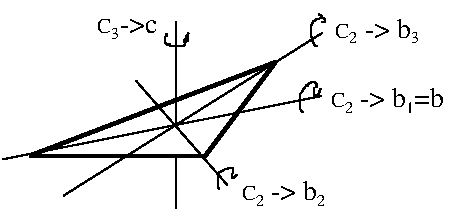
\includegraphics[scale=1.0]{pics/D3}
    \documentclass[border=3mm]{standalone}

\usepackage{tikz}
\usetikzlibrary{arrows.meta,decorations.markings,calc,intersections,backgrounds}

\begin{document}
\begin{tikzpicture}[scale=0.75]
\newcommand{\AxisRotator}[1][rotate=0]{% Defining symbol for axes rotations
    \tikz [x=0.25cm,y=0.60cm,line width=.2ex,-stealth,#1] \draw (0,0) arc (-150:150:1 and 1);%
}

\fill[white] (-6.4,-1.6) -- (-2.2,-1.6) -- (-0.4,0.78) -- cycle;

% Drawing triangle and defining mid-points of each side
\draw[thick] (-6.4,-1.6) coordinate (1)  -- (-2.2,-1.6) coordinate (3) coordinate[pos=0.5] (6);
\draw[thick] (-2.2,-1.6) -- (-0.4,0.78) coordinate[pos=0.5](2);
\draw[thick] (-0.4,0.78)coordinate (5) -- (-6.4,-1.6) coordinate[pos=0.5](4);

% For finding center of triangle
\draw[name path=A] ($(1)!-.2!(2)$) -- ($(2)!-.2!(1)$) node[pos=0.95,scale=0.4,xscale=-1]{\AxisRotator} node[below right] {$C_2 \rightarrow b_1 = b$};
\draw[name path=B] ($(3)!-.4!(4)$) node[below right] {$C_2 \rightarrow b_2$} -- ($(4)!-.4!(3)$) node[pos=0.1,scale=0.4,xscale=-1]{\AxisRotator};

\draw ($(5)!-.3!(6)$) node[below right] {$C_2 \rightarrow b_3$} -- ($(6)!-.4!(5)$) node[pos=0.1,scale=0.4,xscale=-1]{\AxisRotator};
\path[name intersections={of=A and B}] (intersection-1) coordinate (c);
\draw (c) --++ (0,2) node[pos=0.8,rotate=-90,scale=0.4] {\AxisRotator} node[pos=0.8,above left,xshift=-10pt]{$C_3 \rightarrow c$};
\begin{scope}[on background layer]
\draw (c) --++ (0,-2);
\end{scope}
\end{tikzpicture}
\end{document}

    \end{center}
vidimo da su elementi grupe rotacije $e, c$ i  $c^2$ baš kao i kod grupe $\mathrm{C}_3$, te
dodatno rotacije $b_1, b_2$ i $b_3$ za kut 180$^\circ$ oko triju horizontalnih
osi.
\end{primjer}

Uočimo sada neka svojstva množenja u toj grupi. Kao prvo, vrijedi
da je $b_2 = c b_1 c^{-1}$ i kažemo da su $b_2$ i $b_1$ međusobno
\emph{konjugirani} preko elementa $c$. Da je to tako vidi
se iz slike:

\centerline{\documentclass[border=3mm]{standalone}

\usepackage{tikz}
\usetikzlibrary{arrows.meta}

\begin{document}
	\begin{tikzpicture}
		\draw[thick] (-3.1,1.7) node[above] {C} -- (-2.57,0.54) node[below right] {B} -- (-3.79,0.54) node[below left] {A} -- cycle;
		\draw[thick] (-0.3,1.7) node[above] {A} -- (0.23,0.54) node[below right] {C} -- (-0.99,0.54) node[below left] {B} -- cycle;
		\draw[thick] (2.36,1.7) node[above] {C} -- (2.89,0.54) node[below right] {A} -- (1.67,0.54) node[below left] {B} -- cycle;
		\draw[thick] (5.11,1.7) node[above] {A} -- (5.64,0.54) node[below right] {B} -- (4.42,0.54) node[below left] {C} -- cycle;
		\draw[thick] (-3.1,-0.68) node[above] {C} -- (-2.57,-1.84) node[below right] {B} -- (-3.79,-1.84) node[below left] {A} -- cycle;
		\draw[thick] (-0.3,-0.68) node[above] {A} -- (0.23,-1.84) node[below right] {B} -- (-0.99,-1.84) node[below left] {C} -- cycle;
		\draw[-Triangle] (-2.3,1.04) -- (-1.2,1.04) node[above,midway] {$c^{-1}$};
		\draw[-Triangle] (0.37,1.04) -- (1.47,1.04) node[above,midway] {$b_{1}$};
		\draw[-Triangle] (3.12,1.04) -- (4.22,1.04) node[above,midway] {$c$};
		\draw[-Triangle] (-2.3,-1.35) -- (-1.2,-1.35) node[above,midway] {};
		\node at (-4.83,1.04) {$cb_1c^{-1} \quad :$};
		\node at (-4.83,-1.35) {$b_2 \quad :$};
	\end{tikzpicture}
\end{document}}
%\centerline{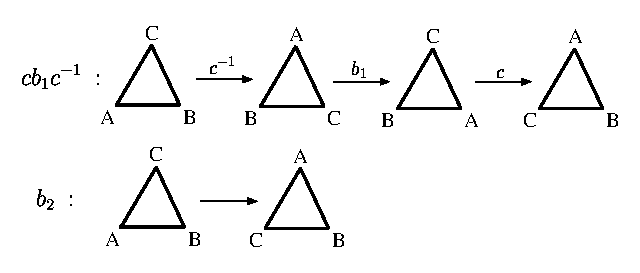
\includegraphics[scale=1.0]{pics/cbc}}

Na sličan način se možemo uvjeriti da je $b_2 = b_1 c $
i $b_3 = b_1 c^2 $, odnosno da 
$c$ i $b\equiv b_1$ generiraju sve ostale transformacije pa
elemente grupe možemo zapisati kao
\begin{equation}
 \{e,c,c^2,b,bc,bc^2\} \;.
\label{eq:d3el}
\end{equation}
To sugerira da bismo grupu D$_3$ mogli probati definirati prezentacijom
\begin{equation}
    {\rm D}_3 \stackrel{?}{=} \langle c, b \: | \: c^3 = b^2 = e \rangle \;,
\label{eq:d3gp1}
\end{equation}
no ova definicija nije kompletna jer nam nedostaje još
i pravilo za komutiranje elemenata (koje nam nije trebalo
za grupu C$_3$ koja je Abelova). Njega dobijemo tako da
iskombiniramo dvije gore dobivene relacije: 
$b_2 = c b_1 c^{-1} = b c$ i pomnožimo zdesna s $c$:
\begin{equation}
c b = b c^2  \;.
\label{eq:d3com}
\end{equation}
Ova relacija sad omogućuje da proizvoljan umnožak elemenata
grupe (npr. $b c b^2 c^5 b$ svedemo na oblik $b^\alpha c^\beta$ gdje
je $\alpha<2$ i $\beta<3$, tj. na jedan od elemenata iz (\ref{eq:d3el}).
Za kompaktan zapis prezentacije grupe D$_3$ koji će se onda moći
lako generalizirati i na ostale D$_n$ grupe, množimo gornju
komutacijsku relaciju (\ref{eq:d3com}) slijeva s $b$ i zdesna s $c$
i dobivamo  $ bcbc \equiv (bc)^2 = b^2 c^3 = e$ pa možemo
pisati
\begin{equation}
 {\rm D}_3= \langle c,b \: | \: c^3 = b^2 = (bc)^2 = e \rangle \;.
\label{eq:d3gp}
\end{equation}
Ova definicija se generalizira na grupu simetrija poligona s $n$
stranica ovako (vidi zadatak \ref{zad:Dn})
\begin{equation}
 {\rm D}_n= \langle c,b \: | \: c^n = b^2 = (bc)^2 = e \rangle \;,
\label{eq:dngp}
\end{equation}
ili, ekvivalentno i praktičnije za komutiranje elemenata prilikom množenja
\begin{equation}
    {\rm D}_n= \langle c,b \: | \: c^n = b^2 = e, cb = b c^{n-1} \rangle \;,
\label{eq:dngpcom}
\end{equation}
što onda sadrži i definiciju grupe
D$_2$ poznate i kao
\emph{Kleinova četvorna grupa} (njem. \emph{Vierergruppe}), 
za koju nemamo odgovarajući poligon kao objekt grupe simetrija.


\section{Podgrupe}
\label{sec:podgrupe}

Za operacije s grupama i njihovu klasifikaciju centralni je pojam \emph{podgrupe}:

\begin{definicija}[Podgrupa]
Podgrupa $H$ grupe $G$ je neprazni podskup $H\subset G$ koji i sam
tvori grupu obzirom na grupnu operaciju definiranu na $G$.
\end{definicija}

Svaka grupa ima trivijalne podgrupe $H=\{e\}$ i $H=G$, a
podgrupu koja je različita od ovih dviju trivijalnih
zovemo \emph{prava} podgrupa.

\begin{primjer} \label{th:c2c3}
C$_2$=\{e, b\} i C$_3$=\{e, c, c$^2$\} su prave podgrupe od D$_3$
\end{primjer}

\begin{primjer}
Grupa translacija i točkasta grupa su podgrupe grupe svih prostornih
simetrija kristala.
\end{primjer}

\begin{definicija}[Susjedna klasa]
Lijeva susjedna klasa (engl. coset) podgrupe $H$ obzirom na element
$g\in G$ je skup
\begin{displaymath}
     gH=\{gh \td h\in H\}
\end{displaymath}
\end{definicija}

Odnos pripadnosti elementa $g_1$ lijevoj susjednoj klasi obzirom na element $g_2$,  
$g_1 \in g_2 H$, uspostavlja \emph{relaciju ekvivalencije}%
\footnote{\label{fn:ekviv}
Općenito, \emph{relacija ekvivalencije} je binarna relacija $a\sim b$ između
elemenata nekog
skupa koja ima slijedeća svojstva
\begin{enumerate}
\item $a\sim a \quad \forall a$ \qquad (refleksivnost)
\item $a\sim b \imp b\sim a$   \qquad (simetričnost)
\item $a\sim b \quad \textrm{i}\quad  b\sim c \imp a\sim c$  \qquad (tranzitivnost)
\end{enumerate}
Primjeri relacija ekvivalencije su: "osoba $a$ je rođena na isti dan kad i osoba $b$"
ili "trokut $a$ je sličan trokutu $b$", dok npr. "broj $a$ je veći ili jednak
broju $b$" nije relacija ekvivalencije jer nije simetrična.
(Ona je antisimetrična. Binarna relacija na skupu koja je refleksivna, antisimetrična
i tranzitivna zove se \emph{relacija uređaja}.)
Svaka relacija ekvivalencije cijepa skup na disjunktne podskupove 
koji se zovu \emph{klase ekvivalencije}.} između ta dva elementa u grupi G, $g_1 \sim g_2$.
To između ostalog znači i da bilo koji element klase možemo jednako koristiti
kao reprezentanta klase tj. da ako je $g_k \in gH$ onda je $g_{k}H = gH$.

Susjedne klase po nekoj podgrupi $H$ su međusobno disjunktne i
zahvaljujući Teoremu o razmještaju sve imaju isti broj elemenata (jednak redu od $H$)
pa tako definiraju jednu particiju grupe G:\\[2ex]
\centerline{\documentclass[border=3mm]{standalone}

\usepackage{tikz}

\begin{document}
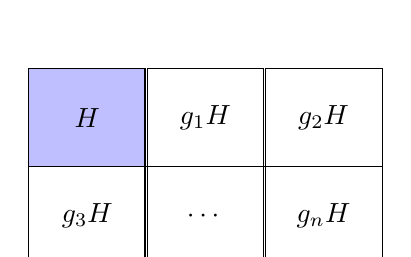
\begin{tikzpicture}
		\node[rectangle,minimum width=1.5cm,minimum height=1.25cm,fill=blue!25,inner sep=0pt](1) {$H$};
		\node[rectangle,minimum width=1.5cm,minimum height=1.25cm,right of=1,node distance=1.5cm](2) {$g_1H$};
		\node[rectangle,minimum width=1.5cm,minimum height=1.25cm,right of=2,node distance=1.5cm](3) {$g_2H$};
		\node[rectangle,minimum width=1.5cm,minimum height=1.25cm,below of=1,node distance=1.25cm](4) {$g_3H$};
		\node[rectangle,minimum width=1.5cm,minimum height=1.25cm,right of=4,node distance=1.5cm](5) {$\cdots$};
		\node[rectangle,minimum width=1.5cm,minimum height=1.25cm,right of=5,node distance=1.5cm](5) {$g_nH$};
		\draw (-0.75,0.625) -- (3.75,0.625) -- (3.75,-1.875) -- (-0.75,-1.875)-- cycle;
		\draw[double] (0.75,0.625) -- (0.75,-1.875);
		\draw[double] (2.25,0.625) -- (2.25,-1.875);
		\draw (-0.75,-0.625) -- (3.75,-0.625);
	\end{tikzpicture}
\end{document}
}
%\centerline{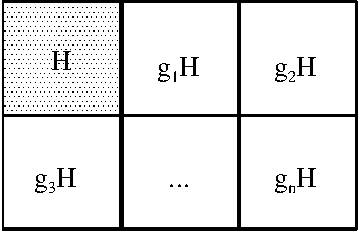
\includegraphics[scale=1.0]{pics/lagrange}}

Na slici je kao prva postavljena lijeva susjedna klasa po jediničnom
elementu $eH = H$. Zbog navedene disjunktnosti klasa i jedinstvenosti
jediničnog elementa ostale susjedne klase naravno ne sadrže jedinični element i
samim time one nisu podgrupe. 
Promatrajući ovu sliku lako se uvjerimo u točnost Lagrangeovog
teorema:

\begin{teorem}[Lagrange]
Red podgrupe dijeli red grupe.
\end{teorem}

Tako u Primjeru \ref{th:c2c3} redovi podgrupa C$_2$ i C$_3$, 2 i 3, dijele red
grupe D$_3$, 6. Skup čiji su elementi predstavljeni kvadratičima na gornjoj slici
ima svoj naziv:

\begin{definicija}[Kvocijentni skup]
Skup svih različitih lijevih susjednih klasa 
\begin{displaymath}
      G/H \equiv \{gH \td g\in G\}
\end{displaymath}
zove se \emph{lijevi kvocijentni skup} grupe $G$ po podgrupi $H$.
\end{definicija}

Potpuno analogno se definiraju \emph{desna susjedna klasa} $Hg$
i \emph{desni kvocijentni skup} $H\backslash G$.

\begin{primjer}[D$_3$]
    Promotrimo podgrupu $H=\mathrm{C}_3=\{e, c, c^2\}$ grupe $G=\mathrm{D}_3$.
Dvije lijeve susjedne klase su
\begin{enumerate}
\item $eH=H=\{e, c, c^2\}$ \; \text{i}
\item $bH=\{b, bc, bc^2\}$ \;,
\end{enumerate}
a kvocijentni skup je $\mathrm{D}_3/\mathrm{C}_3=\{eH, bH\}$. Postoji i kvocijentni 
skup $\mathrm{D}_3/\mathrm{C}_2$
\end{primjer}

\begin{definicija}[Normalna podgrupa]
Podgrupa za koju vrijedi $gH=Hg$, $\forall g\in G$, zovemo
\emph{normalna} ili \emph{invarijantna}.
\label{tm:normalnapodgrupa}
\end{definicija}

\begin{primjer}[$\mathrm{D}_3$]
    $G=\mathrm{D}_3$, $H=\mathrm{C}_3$. Eksplicitnim množenjem se uvjerimo da
    je $b\mathrm{C}_3 = \mathrm{C}_3 b$, a za ostale elemente $g\in \mathrm{D}_3$ jednakost
    lijevih i desnih susjednih klasa je trivijalna.
    Dakle, $\mathrm{C}_3$  je normalna podgrupa od $\mathrm{D}_3$. S druge strane
    $\mathrm{C}_2 = \{e, b\}$ nije normalna podgrupa od $\mathrm{D}_3$
    jer npr. $c \mathrm{C}_2 \neq \mathrm{C}_2 c$.
\end{primjer}

Očito je da su za normalnu podgrupu $H$ lijevi i desni kvocijentni skupovi
identični  $G/H$ = $H\backslash$G.

Zanimljivo je pitanje u kojim okolnostima i sam kvocijentni skup čini grupu.
Za to je potrebno definirati binarnu operaciju elemenata kvocijentnog
skupa tj. "množenja" susjednih klasa.
Prirodno je pokušati s definicijom množenja dvije klase $A$ i 
$B$ "svaki element sa svakim":
\begin{equation}\label{eq:ABmult}
    A B =\{ab \td a \in A \:\text{i}\: b \in B\} \;.
\end{equation}
Pitanje je međutim predstavlja li ovako definirano množenje skupova $A$ i $B$
konzistentnu definiciju množenja susjednih klasa tj. je li $AB$ nužno susjedna
klasa, ukoliko su to $A$ i $B$? To zahtijeva prvi aksiom definicije
grupe. Lako se možemo uvjeriti da tako definirano množenje \emph{ne} funkcionira
na kvocijentnom skupu $\mathrm{D}_3 / \mathrm{C}_2$, gdje je $\mathrm{C}_2 = \{e, b\}$.
Npr. umnožak susjednih klasa $e\mathrm{C}_2 = \{e, b\}$ i $c\mathrm{C}_2=\{c, bc^2\}$
je $\{e, bc, bc^2, b^2 c^2 = c^2\}$ što je skup koji nije susjedna klasa!
S druge pak strane množenje susjednih klasa u kvocijentnom skupu
$\mathrm{D}_3 / \mathrm{C}_3$ uvijek rezultira susjednom klasom. Razlog tome je
što je $\mathrm{C}_3$ \emph{normalna} podgrupa, a za normalnu podgrupu $H$ 
množenje klasa možemo provesti kao:
\begin{equation}
       (g_1H)(g_2H) = g_1 (H g_2) H = g_1 (g_2 H) H = g_1 g_2 H H
       = (g_1 g_2) H\;,
\end{equation}
gdje smo u drugom koraku iskoristili normalnost podgrupe $H$ i gdje je
$(g_1 g_2) H$ nužno susjedna klasa jer je $g_1 g_2 \in G$.
Lako se uvjeriti da su i ostali aksiomi grupe zadovoljeni pa zaključujemo
da kvocijentni skup po normalnoj podgrupi čini grupu koju zovemo
\emph{kvocijentna grupa}\footnote{Nešto je teže
    uvjeriti se u činjenicu da bi i drugačiji pokušaji definiranja množenja
    susjednih klasa od (\ref{eq:ABmult}) doveli do nužnosti da podgrupa
bude normalna. Npr. mogli bismo umjesto oslanjanja na (\ref{eq:ABmult}) 
\emph{definirati} množenje susjednih klasa kao $(g_1 H) \ast (g_2 H) = (g_1 g_2) H$.
Tako bi prvi aksiom grupe naizgled bio osiguran samom definicijom binarne operacije.
No pokazuje se da je ovakva definicija množenja susjednih klasa konzistentna, u smislu
da ne ovisi o izboru reprezentirajućih elemenata $g_1$ i $g_2$, i opet samo ako je
podgrupa normalna, nakon čega ta definicija postaje ekvivalentna definiciji (\ref{eq:ABmult}).}


\begin{primjer}[$\mathrm{D}_{3}$/$\mathrm{C}_3$]
Tablica množenja u ovom kvocijentnom skupu je dana relacijama
\begin{align}
    (e\mathrm{C}_3)(e\mathrm{C}_3) &= ee \mathrm{C}_3 = e\mathrm{C}_3\\
    (e\mathrm{C}_3)(b\mathrm{C}_3) &= b\mathrm{C}_3  \\
    (b\mathrm{C}_3)(e\mathrm{C}_3) &= b\mathrm{C}_3  \\
    (b\mathrm{C}_3)(b\mathrm{C}_3) &= e\mathrm{C}_3 
\end{align}

Lijevi i desni kvocijentni skupovi su jednaki
\begin{align*}
{\rm D}_{3}/{\rm C}_3 &= \{\{e,c,c^2\}, \{b, bc, bc^2\}\} \\
{\rm C}_3\backslash{\rm D}_{3} &= \{\{e,c,c^2\}, \{b, cb=bc^2, c^2b=bc\}\}
    = D_{3}/C_3
\end{align*}
i imaju grupnu strukturu jednaku grupi $\mathrm{C}_2$.
\label{pr:D3oC3}
\end{primjer}

S druge strane $\mathrm{C}_2$ nije normalna, lijevi i desni kvocijentni
skupovi
\begin{align*}
{\rm D}_{3}/{\rm C}_2 &= \{\{e,b\}, \{c, cb=bc^2\}, \{c^2, c^2b=bc\}\} \\
{\rm C}_2\backslash{\rm D}_{3} &= \{\{e,b\}, \{c, bc\}, \{c^2, bc^2\}\}
    \neq {\rm D}_{3}/{\rm C}_2
\end{align*}
nisu jednaki i $\mathrm{D}_{3}$/$\mathrm{C}_2$ nije grupa.

Grupe koje nemaju normalnih podgrupa zovu se \emph{jednostavne}\footnote{Mi se
    nećemo baviti simetrijama algebarskih jednadžbi, ali spomenimo
    da je \'{E}variste Galois povezao njihovu općenitu rješivost (mogućnost
    da se sva rješenja prikažu u obliku izraza koji uključuju konačni broj
    primjena osnovnih matematičkih operacija i korijena na
    koeficijente jednadžbe) s nejednostavnošću pripadajuće grupe simetrija
    skupa rješenja. Onda je dokazavši da su grupe simetrija skupa rješenja za jednadžbe reda
    većeg od 5 jednostavne pokazao da te jednadžbe nisu rješive. To je otkriće predstavljalo
kraj teorije algebarskih jednadžbi i rođenje teorije grupa.\label{fus:galois}} ,
a one koje nemaju normalnih Abelovih podgrupa zovu se \emph{polujednostavne}.

Za normalne grupe iz definicije \ref{tm:normalnapodgrupa} slijedi odmah i
da je $g H g^{-1} = H, \forall g\in G$. Zanimljivo je promatrati djelovanje
ove operacije $g \ldots g^{-1}$ i na skupove koji nisu podgrupa te
na pojedine elemente grupe:

\begin{definicija}[Konjugirani elementi]
Dva elementa $a$ i $b$ grupe $G$ su \emph{konjugirani} ukoliko
postoji $g\in G$ takav da je $a=gbg^{-1}$.
\label{tm:konjugacija}
\end{definicija}

Konjugacija je također relacija ekvivalencije:
\begin{enumerate}
\item $a=e^{-1} a e  \imp a\sim a$
\item $a=g^{-1} b g  \imp  b= g^{-1} a (g^{-1})^{-1}$
\item $a=g b g^{-1}$, $b=hch^{-1}$, \\
         $a=ghch^{-1}g^{-1}=(gh)c(gh)^{-1}$, $gh\in G$
  
\end{enumerate}


Konjugacija (baš kao i svaka relacija ekvivalencije) definira
particiju skupa na klase.
\begin{displaymath}
   \text{klasa od $a$} = \{ b \td b=gag^{-1},\quad g\in G\}
\end{displaymath}

Klasa od $e=\{e\}$ što znači da klase, izuzev ove trivijalne, nisu podgrupe.

Za Abelove grupe svaki element je klasa za sebe.

Kako normalne podgrupe zadovoljavaju $gHg^{-1}=H$, $\forall g\in G$, slijedi
da su one sastavljenje od \emph{cijelih} klasa konjugacije.

\begin{primjer}[Klase konjugacije grupe D$_3$] \label{pr:klaseD3}
Tri klase konjugacije  od D$_3$ su:
\begin{enumerate}
\item $(e)$
\item $(c, c^{2})$
\item $(b, bc, bc^2)$
\end{enumerate}
i odgovaraju rotacijama za različite kutove: $0^\circ$, $120^\circ$ i
$180^\circ$. Konjugirajući elementi
preslikavaju međusobno osi rotacije. Normalna podgrupa $\mathrm{C}_3$ se
sastoji od cijelih klasa (prve dvije), dok podgrupa $\mathrm{C}_2=\{e,b\}$ nema
to svojstvo i nije normalna.
\end{primjer}

\section{Homomorfizam i izomorfizam grupa}

Vidjeli smo u primjeru \ref{pr:D3oC3} kako kvocijentna grupa $\mathrm{D}_3/\mathrm{C}_3$
ima isti broj elemenata i istu tablicu množenja kao grupa $\mathrm{C}_2$. Dakle u
apstraktnom smislu teorije grupa te su grupe identične.  Za prepoznavanje takvih
situacija, umjesto uspoređivanja grupnih tablica množenja pogodnije je identificirati
preslikavanje s jedne grupe na drugu koje "čuva" grupnu binarnu operaciju. Takvo preslikavanje
se naziva \emph{homomorfizam}:
\begin{definicija}[Homomorfizam]
Neka su $A$ i $B$ grupe, a $f:A\to B$ preslikavanje koje komutira
s grupnom operacijom tj. za koje vrijedi
\begin{displaymath}
      f(ab)=f(a)f(b) \quad \forall a,b\in A \;.
\end{displaymath}
Onda kažemo da je $f$ \emph{homomorfizam} grupe $A$ u grupu $B$.
\end{definicija}

\begin{primjer}
    Preslikavanje s grupe $\mathrm{D}_3$ na kvocijentnu grupu
    $\mathrm{D}_3/\mathrm{C}_3$ definirano kao 
    \[
        f(g) = g\mathrm{C}_3 \,,
    \] je homomorfizam jer
    \[
        f(a) f(b) = (a \mathrm{C}_3) (b \mathrm{C}_3 ) =
        (a b) \mathrm{C}_3 = f(a b)
    .\] 
\end{primjer}
\begin{primjer}
    Preslikavanje s grupe $\mathrm{C}_3$ na trivijalnu grupu $\mathrm{C}_1 = \{e\}$
    koja sadrži samo jedinični element, definirano kao $f(g) = e,
    \forall g\in\mathrm{C}_3$, je homomorfizam.
    \label{pr:C3toC1}
\end{primjer}

Vidimo da homomorfizam općenito ne mora biti injekcija tj. da se više
elemenata može preslikavati u isti element.
Homomorfizam koji je i bijekcija zovemo \emph{izomorfizam} i
pišemo $A\cong B$ ili $A=B$.

Izomorfne grupe su s apstraktnog stanovišta jednake (imaju
istu tablicu množenja).

\begin{primjer}
Grupa C$_2$ je, osim već spomenutog izomorfizma s
kvocijentnom grupom $\mathrm{D}_3/\mathrm{C}_3$, izomorfna i
npr. s grupama 
$$
(\{1, -1\},\cdot) \qquad \text{i} \qquad \left(\left\{
\begin{pmatrix}
1 & 0 \\ 0 & 1
\end{pmatrix},
\begin{pmatrix}
0 & 1 \\ 1 & 0
\end{pmatrix}
\right\},\cdot\right)\,.$$
\end{primjer}

\begin{primjer}
    Grupa $\mathbb{Z}_n$ je skup cijelih brojeva $\{0, 1, 2, \ldots, n-1\}$,
    uz binarnu operaciju zbrajanja modulo $n$. Jedinični element je naravno 0,
    a cijelu grupu generira element 1 i grupa je izomorfna cikličkoj grupi $\mathrm{C}_n$.
    Stoga mnogi autori cikličke grupe označavaju $\mathbb{Z}_n$, a u primjenama u fizici
    se često sreće $\mathrm{C}_2$ koju ćemo onda i mi zbog sklada s literaturom
    nekad zvati $\mathbb{Z}_2$.
\end{primjer}

\emph{Slika} homomorfizma $f(A)$ (skup svih elemenata u $B$ koji imaju original u $A$) 
je podgrupa od $B$. Uvjerite se u to.


\begin{figure}[htpb]
    \centering
    \documentclass[border=3mm]{standalone}

\usepackage{tikz}
\usetikzlibrary{arrows.meta,shapes}

\begin{document}
	\begin{tikzpicture}
		\node[ellipse,draw,thick,minimum width=2.55cm,minimum height=5.325cm,inner sep=0pt,label={above:$A$}] (1) at (-2.83,-0.65) {};
		\node[ellipse,draw,thick,minimum width=2.55cm,minimum height=5.325cm,inner sep=0pt,label={above:$B$}] (2) at (3.13,-0.65) {};
		\node[ellipse,draw,thick,minimum width=1cm,minimum height=2.1cm,inner sep=0pt,fill=blue!25] (3) at (-2.87,-0.71) {$K$};
		\node[ellipse,draw,thick,minimum width=1.5cm,minimum height=3.65cm,inner sep=0pt,fill=blue!25] (4) at (3.13,-0.65) {};
		\node[circle,fill=black,inner sep=0pt,minimum size=6pt,label={above:$e$}](5) at (3.19,-0.65) {};
		\node at (3.1,-1.5) {$f(A)$};
		\draw (1.north) -- (4.north);
		\draw (1.south) -- (4.south);
		\draw (3.north) -- (5.north west);
		\draw (3.south) -- (5.south west);
		\node at (3.1,-1.5) {};
		\draw[-Triangle] (-2.07,2.3) -- (2.34,2.3) node[above,midway] {$f$};
	\end{tikzpicture}
\end{document}
    %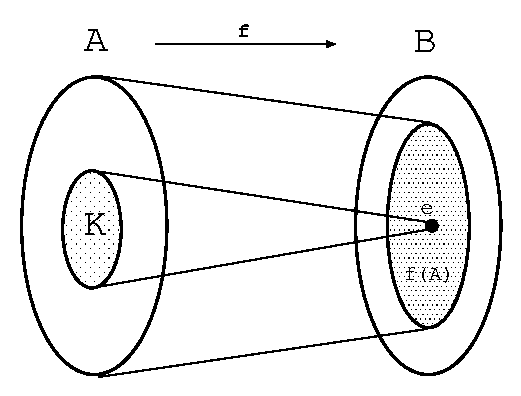
\includegraphics[width=0.6\textwidth]{pics/homomorfizam}
    \caption{Kernel $K$ homomorfizma $f:A\to B$ je podgrupa grupe $A$,
    a slika $f(A)$ homomorfizma je podgrupa grupe $B$.}
    \label{fig:kernelslika}
\end{figure}


Slika $f(e_A)$ jediničnog elementa $e_A$ iz $A$ je jedinični element $e_B$ u $B$ jer
množenjem relacije
$$ f(e_A) f(b) = f(e_A b) = f(b) $$
s desna s $f(b)^{-1}$ dobivamo
$$ f(e_A) = f(b) f(b)^{-1} = e_B \;. $$
No moguće je da se i drugi elementi iz $A$ osim jediničnog $e_A$ preslikavaju u 
jedinični element $e_B$ u $B$ (u primjeru \ref{pr:C3toC1} se svi tako preslikavaju).
\emph{Kernel} homomorfizma se naziva skup svih elemenata od $A$ koji se
preslikavaju u jedinični element iz $B$.
$$ K \equiv {\rm ker}(f) \equiv \{ k\in A \; | \; f(k) = e_B \} \;. $$
Kernel od $f:A\to B$ je normalna podgrupa od $A$. Uvjerite se u to.

Kernel je iznimno korisna podgrupa, između ostalog i zahvaljujući sljedećem
važnom teoremu:
\begin{teorem}[Teorem o izomorfizmu]
\label{th:izomorfizam}
Ako je $f:G\to G'$ homomorfizam s kernelom $K$, onda vrijedi
\begin{enumerate}
\item Svaki element susjedne klase $gK$ se preslikava u isti element $f(g)$.
\item Slika homomorfizma $f(G)$ je izomorfna kvocijentnoj grupi po kernelu $G/K$.
\end{enumerate}
\end{teorem}
(Skup $G/K$ je grupa jer je $K$ normalna podgrupa.)

\emph{Dokaz}$^{*}$\secret{Cornwell '84, 2.6}: Pridruživanje koje
čini izomorfizam iz stavka 2) teorema je $f(g)\leftrightarrow gK$.
Pokažimo da je to pridruživanje dobro definirano i bijekcija te da čuva grupnu
strukturu.
Da bi se uvjerili da je pridruživanje $f(g)\mapsto gK$ dobro definirano, treba
se uvjeriti da je susjedna klasa $gK$ jedinstveno određena izborom $f(g)$. Naime,
postoji opasnost da različiti originali od $f(g)$ ne pripadaju istoj klasi
kako je ilustrirano na\\[2ex]
\vspace*{3ex}
\centerline{\documentclass[border=3mm]{standalone}

\usepackage{tikz}
\usetikzlibrary{decorations.markings,arrows.meta}

\begin{document}
	\begin{tikzpicture}
		\draw[thick]  (-1.93,-0.52) ellipse (1 and 1.92);
		\draw[thick]  (2.51,-0.52) ellipse (1 and 1.92);
		\draw[fill=blue!25]  (-1.95,-0.29) ellipse (0.46 and 0.81);
		\node[circle,fill=black,inner sep=0pt,minimum size=4pt,label={left,xshift=2pt:$g$}] (1) at (-1.93,0.06) {};
		\node[circle,fill=black,inner sep=0pt,minimum size=4pt,label={below,xshift=2pt:$f(g)$}] (2) at (2.48,0.25) {};
		\node[circle,fill=black,inner sep=0pt,minimum size=4pt,label={ left,xshift=2pt:$?g'$}] (3) at (-1.78,-1.58) {};
		\node at (-1.9,-0.7) {$gK$};
	\begin{scope}[decoration={
		markings,
		mark=at position 0.5 with {\arrow{Triangle}}
	}]
		\draw[postaction={decorate}] (1) -- (2);
		\draw[postaction={decorate}] (3) -- (2);
	\end{scope}
	\end{tikzpicture}
\end{document}}
%\centerline{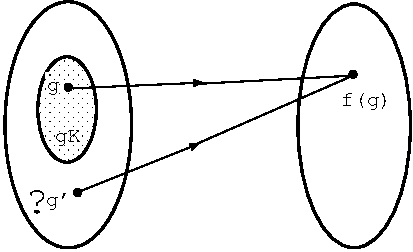
\includegraphics[scale=0.8]{pics/homo1}}
No, različiti originali od $f(g)$, dakle $g$ i $g'$ iz $G$
takvi da je  $f(g)=f(g')$ zadovoljavaju
$f(g^{-1} g')=f(g^{-1})f(g')=f(g)^{-1}f(g')=f(g)^{-1}f(g)=e$ što  znači
da je $g^{-1} g'$ jednak nekom elementu $k$ kernela od $f$,
$g^{-1} g' \equiv k\in K$ što množenjem s $g$ slijeva
daje $g'=gk$ pa je nužno $g' \in gK$.


Druga opasnost je da inverzno pridruživanje
$gK\mapsto f(g)$ ovisi o izboru elementa $g$ iz $K$ tj. da
se različiti elementi klase $gK$ ne preslikavaju u isti $f(g)$
kako je ilustrirano na\\[2ex]
\vspace*{3ex}
\centerline{\documentclass[border=3mm]{standalone}

\usepackage{tikz}
\usetikzlibrary{decorations.markings,arrows.meta}

\begin{document}
	\begin{tikzpicture}
		\draw[thick]  (-2.13,-0.12) ellipse (1 and 1.92);
		\draw[thick]  (2.31,-0.12) ellipse (1 and 1.92);
		\draw[fill=blue!25]  (-2.22,-0.11) ellipse (0.55 and 1.);
		\node[circle,fill=black,inner sep=0pt,minimum size=4pt,label={left,xshift=2pt:$g$}] (1) at (-2.13,0.46) {};
		\node[circle,fill=black,inner sep=0pt,minimum size=4pt,label={below,xshift=2pt:$f(g)$}] (2) at (2.28,0.65) {};
		\node[circle,fill=black,inner sep=0pt,minimum size=4pt,label={ left,xshift=2pt:$g'$}] (3) at (-2.13,-0.27) {};
		\node[circle,fill=black,inner sep=0pt,minimum size=4pt,label={right,align=center:$f(g')$\\?}] (4) at (2.05,-0.97) {};
		\node at (-2.17,-0.85) {$gK$};
	\begin{scope}[decoration={
		markings,
		mark=at position 0.5 with {\arrow{Triangle}}
	}]
		\draw[postaction={decorate}] (1) -- (2);
		\draw[postaction={decorate}] (3) -- (4);
	\end{scope}
	\end{tikzpicture}
\end{document}}
%\centerline{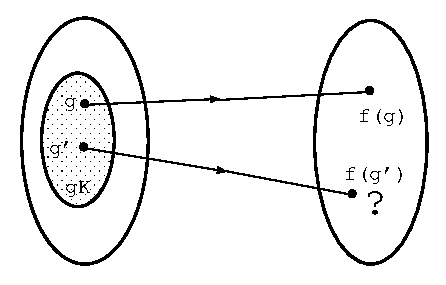
\includegraphics[scale=0.8]{pics/homo2}}
No različiti element $g'$ iz susjedne klase $gK$ je oblika $g'=gk$ za neki
$k\in K$ što znači da je $g^{-1} g'\in K$ i mora se preslikavati
u jedinični element
$f(g^{-1}g')=e$ pa po svojstvu homomorfizma $f$ imamo 
$f(g)^{-1}f(g')=e$ i množenjem slijeva s $f(g)$ dobivamo željeno
svojstvo $f(g')=f(g)$, čime istovremeno i dokazujemo prvi dio teorema.

Injekcija u oba smjera koju smo upravo dokazali znači da je
preslikavanje $f(g)\leftrightarrow gK$ bijekcija. Potrebno je još samo
uvjeriti se da to preslikavanje čuva grupno množenje. To se vidi iz toga
što se umnožak elemenata slike homomorfizma $f(g)f(g')=f(gg')$ preslikava
u susjednu klasu $(gg')K$ koja je po svojstvu normalnosti kernela jednaka
odgovarajućem množenju $(gK)(g'K)$ u kvocijentnoj grupi $G/K$.
Dakle $f(g)\leftrightarrow gK$ je izomorfizam.\qed
  

\secret{Primjer: $D_3$: $C_3\to e$, a ostali u $c$ iz $C_2$
 $\imp f(D_3) = C_2 = D_3/C_3$}

Jedan korolar ovog teorema je da je svaki element $g'$ iz $G'$ slika
istog broja elemenata iz $G$ (jer vidjeli smo da sve susjedne klase po
nekoj podgrupi imaju isti broj elemenata). Tako općeniti homomorfizam
ima vrlo pravilni obrazac preslikavanja prikazan na sljedećoj slici\\[2ex]
\vspace*{4ex}
\centerline{\documentclass[border=3mm]{standalone}

\usepackage{tikz}
\usetikzlibrary{decorations.markings,arrows.meta}

\begin{document}
	\begin{tikzpicture}[scale=1.5]
		\tikzstyle{dot}=[circle,fill,inner sep=0pt,outer sep=1pt,minimum size=3pt]
		\draw[thick] (-1.6196,-0.1149) ellipse (0.72 and 2.05);
		\draw[thick] (2.0788,-0.1149) ellipse (0.72 and 2.05);
		\node[dot] (1) at (-1.5933,1.5) {};
		\node[dot] (2) at (-1.6,1.2) {};
		\node[dot] (3) at (-1.6,0.9) {};
		\node[dot] (4) at (-1.6,0.6) {};
		\node[dot] (5) at (-1.6,0.3) {};
		\node[dot] (6) at (-1.6,0) {};
		\node[dot] (7) at (-1.6,-0.3) {};
		\node[dot] (8) at (-1.6,-0.6) {};
		\node[dot] (9) at (-1.6,-0.9) {};
		\node[dot,label={right:$e$}] (a) at (2.0737,1.2) {};
		\node[dot] (b) at (1.9,0.3) {};
		\node[dot] (c) at (2.2,-0.6) {};
		\node at (-1.667,-1.5) {$\cdots$};
		\node at (2.1,-1.6) {$\cdots$};
		\draw  (-1.6,1.22) ellipse (0.18 and 0.5) node[left,xshift=-7pt]{$K$};
		\draw[-{Triangle[scale=0.75]}] (1) -- (a);
		\draw[-{Triangle[scale=0.75]}] (2) -- (a);
		\draw[-{Triangle[scale=0.75]}] (3) -- (a);
		\draw[-{Triangle[scale=0.75]}] (4) -- (b);
		\draw[-{Triangle[scale=0.75]}] (5) -- (b);
		\draw[-{Triangle[scale=0.75]}] (6) -- (b);
		\draw[-{Triangle[scale=0.75]}] (7) -- (c);
		\draw[-{Triangle[scale=0.75]}] (8) -- (c);
		\draw[-{Triangle[scale=0.75]}] (9) -- (c);
	\end{tikzpicture}
\end{document}}
%\centerline{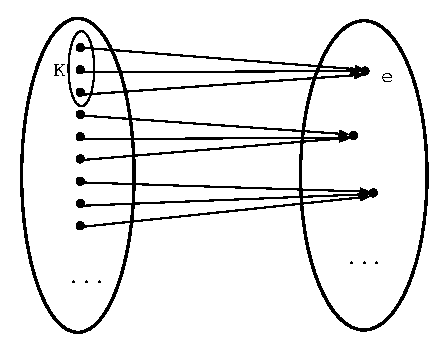
\includegraphics[scale=1.0]{pics/homo3}}
Drugi korolar je da je $f$ izomorfizam ako i
samo ako je kernel $K=\{e\}$.

Pojam kvocijentne grupe nam daje ideju svojevrsnog "dijeljenja" jedne
grupe drugom.
Nameće se pitanje, ukoliko je, kako smo vidjeli, 
$\mathrm{D}_{3}$/$\mathrm{C}_3 = \mathrm{C}_2$, možemo li u nekom smislu
smatrati da je $\mathrm{C}_3 \times \mathrm{C}_2 = \mathrm{D}_3$?
Odgovor je da to nije moguće općenito, ali jest u situaciji kad su
\emph{obje} grupe normalne podgrupe produktne grupe, što u primjeru
$\mathrm{D}_3$ nije slučaj.

\begin{definicija}[Direktni produkt grupa]\label{def:direktniproduktgrupa}
Ako imamo dvije grupe (G, $\star$) i (H, $\circ$), onda je njihov
\emph{direktni produkt} grupa G$\times$H čiji su elementi svi uređeni
parovi $(g, h)$, $g \in \mathrm{G}$, $h \in \mathrm{H}$, a 
binarna operacija $\cdot$ je definirana prirodno po komponentama
\begin{equation}
    (g_1, h_1) \cdot (g_2, h_2) = (g_1 \star g_2, h_1 \circ h_2) \,.
    \label{eq:Gproduct}
\end{equation}
\end{definicija}

Lako se uvjeriti da su zadovoljeni svi aksiomi grupe. Strogo 
uzevši, gore tražene normalne podgrupe od G$\times$H nisu baš G i H nego
    $\mathrm{G}' = \{ (g, 1) \td g \in G \}$ i
    $\mathrm{H}' = \{ (1, h) \td h \in H \}$,
ali one su izomorfne grupama G i H pa je sve prirodno i konzistentno.
Čitaoc se lako može uvjeriti da je na primjer
$\mathrm{C}_2 \times \mathrm{C}_2 = \mathrm{D}_2$.

\subsection*{Zadaci}

\begin{enumerate}[label=\arabic{chapter}.\arabic*.]
\item Dokažite da su jedinični i inverzni element grupe jedinstveni.
\item Konstrukcijom grupne tablice množenja pokažite da postoji samo
jedna grupa reda 3.
\item Na isti način kao u prošlom zadatku pokažite da postoje samo
dvije grupe reda 4.
\item Grupa je Abelova ako i samo ako je njena grupna tablica množenja simetrična.
Dokažite da i za grupe koje nisu Abelove razmještaj jediničnih elemenata u tablici
mora biti simetričan.
\item Dokažite da je grupa u kojoj je svaki element samom sebi inverz nužno Abelova.
\item Uvjerite se da je grupa simetrija pravilnog poligona s $n$ neusmjerenih
    stranica izomorfna grupi $\mathrm{D}_n=\langle c,b \td c^n = b^2 = (bc)^2 = e \rangle $.
    (\emph{Naputak}: Odredite transformacije poligona koje odgovaraju elementima $c$ i
 $b$, pa se uvjerite da one zadovoljavaju $c^n = b^2 = (bc)^2 = e$. Usporedite
broj elementa grupa.)\label{zad:Dn}
\item \label{zad:centar} Centar $Z$ grupe $G$ je skup svih elemenata koji komutiraju sa svakim
elementom grupe tj. $Z=\{z\in G \td zg=gz \; \forall g\in G\}$. Pokažite da
je $Z$ normalna Abelova podgrupa od $G$.
\item Odredite klase konjugacije grupe D$_4$.
\item Pokažite da su sve grupe s prostim brojem elemenata cikličke.
\item \emph{Red} elementa $a$ grupe $G$ je najmanji $n$ takav da je $a^n=e$.
    Pokažite da je red svih elemenata jedne klase konjugacije isti.\label{zad:redel}
\item Postoji li netrivijalni homomorfizam s grupe D$_4$ na grupu D$_3$?
\item Pokažite da je kvocijentna grupa $\mathbb{Z}/\mathbb{Z}_e$
izomorfna grupi C$_2$, gdje je $\mathbb{Z}_e$ grupa parnih cijelih brojeva.
\item Promotrite grupu nesingularnih kvadratnih $n\times n$ 
matrica $G=\{M\}$. Pokažite da je $f(M)=\det M$ homomorfizam.
Koja grupa je kodomena tog homomorfizma?
\end{enumerate}

% Correcting the title chapter page
\fancypagestyle{plain}{%
    \fancyhf{}
    \fancyhead[RO,LE]{\bfseries \thepage}
    \fancyhead[CO]{\rightmark}
    \fancyhead[CE]{\leftmark}
    \renewcommand{\headrulewidth}{0.4pt}}

\chapter{Reprezentacije grupa}

Premda smo glavne primjere grupa u prošlom poglavlju,
cikličke grupe $\mathrm{C}_n$ i dihedralne grupe $\mathrm{D}_n$,
definirali kao grupe simetrija poligona,
naglašavali smo da je to samo pomoćni korak i da je stvarna
narav grupe apstraktna, potpuno definirana svojstvima binarne
operacije nad elementima skupa.
No prava moć teorije grupa, i ne samo u fizici, ipak dolazi kroz
konkretne realizacije grupe kao skupa transformacija
nekog sustava. Za te potrebe, sustave ćemo
prikazivati kao elemente vektorskih prostora, a elementi
grupe će biti operatori nad tim prostorima.
To pokriva sve važne situacije u fizici, a najvažnije
i najnetrivijalnije primjene bit će u \emph{kvantnoj} fizici gdje
je odgovarajući vektorski prostor Hilbertov prostor kvantnomehaničkih
stanja. Najvažnije pitanje kojim ćemo se baviti je određivanje na koje je
sve načine moguće reprezentirati neku grupu kao skup operatora nad
nekim prostorom.
To će onda dati jednu važnu klasifikaciju sustava a time i odgovor na pitanje
na koje se sve načine neka simetrija može javljati u prirodi.



\section{Vektorski prostori i operatori na njima}

Očekuje se da je čitaoc već upoznat s osnovama matematičke
teorije vektorskih prostora, no u ovom ćemo odjeljku ipak ponoviti
osnovne pojmove.

\begin{definicija}[Vektorski prostor]
Vektorski prostor (ili linearni prostor) $V$ nad poljem $F$ je aditivna grupa
(grupna operacija je zbrajanje vektora $\vec{x}+\vec{y}$) na
kojoj je definirana operacija \emph{množenja skalarom} iz $F$ tako
da su zadovoljeni aksiomi:
\begin{enumerate}
\item Zatvorenost: $a\vec{x}\in V \quad \forall a\in F,\; \vec{x}\in V$
\item Kvaziasocijativnost: $a(b\vec{x})=(ab)\vec{x} \quad
 \forall a,b \in F,\; \vec{x}\in V$
\item Egzistencija jedinice: $ 1\vec{x}=\vec{x} \quad \text{za}\; 1\in F
 \;\text{i}\; \forall \vec{x} \in V $
\item Distributivnost zbrajanja u $F$:
 $(a+b)\vec{x} = a \vec{x} + b \vec{x} \quad \forall a,b \in F,\;\vec{x} \in V$
\item Distributivnost zbrajanja u $V$:
 $a(\vec{x} + \vec{y}) = a \vec{x} + a \vec{y} \quad \forall a \in F,\; 
 \vec{x}, \vec{y} \in V$
\end{enumerate}
\end{definicija}

Iz aksioma slijedi da je zbrajanje vektora u $V$  komutativno tj.
 $\vec{x} + \vec{y} = \vec{y} + \vec{x} $.
Za naše potrebe, polje $F$ je obično polje kompleksnih ili 
realnih brojeva, $\mathbb{C}$ ili $\mathbb{R}$, pa govorimo o
 \emph{kompleksnom} ili \emph{realnom} vektorskom prostoru.
\emph{Baza} vektorskog prostora je skup $\{\vec{e}_{i}\}$ linearno nezavisnih vektora koji 
\emph{razapinju} $V$ tj. svaki vektor iz $V$ se može prikazati kao linearna
 kombinacija vektora baze $\{\vec{e}_{i}\}$.
\emph{Dimenzija} vektorskog prostora definirana je kao broj vektora njegove baze (teorem
je da sve baze imaju isti broj vektora).

\begin{primjer}[3D euklidski prostor]
Riječ je o "klasičnom" realnom vektorskom prostoru u kojem vrijedi osnovnoškolska
geometrija. Jedna moguća baza je Kartezijeva
$\vec{e}_{1}=\hat{\vec{x}}, \vec{e}_{2}=\hat{\vec{y}}, 
   \vec{e}_{3}=\hat{\vec{z}}$, tako da je
\begin{equation}
    \vec{r} = x \hat{\vec{x}} + y \hat{\vec{y}} + z \hat{\vec{z}} \;.
\end{equation}
Proizvoljni vektor često prikazujemo i kao stupac njegovih triju komponenata
u konkretnoj bazi:
\begin{equation}
\vec{r}= \left(
\begin{array}{c}
x \\
y \\
z
\end{array} \right) \;.
\end{equation}
\end{primjer}

\begin{primjer}[Hilbertov prostor kvantnomehaničkih stanja vodikovog atoma]

Rješenja vremenski nezavisne Schr\"{o}dingerove diferencijalne jednadžbe 
\begin{equation}
H\psi(\vec{x})=E\psi(\vec{x}) \;,
\end{equation}
gdje je $H$ hamiltonijan za vodikov atom, označavamo 
$\psi_{nlm}(\vec{x})$ i nazivamo stacionarna stanja. Ovdje je
$m \in \{-l, -l+1, \ldots, l\}$, $l \in \{0, 1, \ldots, n-1\}$,
a $n \in \{1, 2, \ldots, \infty\}$. Stacionarnih stanja ima
beskonačno i ona predstavljaju
bazu beskonačnodimenzionalnog Hilbertovog vektorskog prostora
svih mogućih kvantnomehaničkih stanja vodikovog atoma.
Vektor u tom prostoru je proizvoljna superpozicija stacionarnih
stanja
\begin{equation}
       \psi(\vec{x})=\sum_{n=1}^{\infty}\sum_{l=0}^{n-1}
  \sum_{m=-l}^{l}  a_{nlm}  \psi_{nlm}(\vec{x}) \;,
\end{equation}
gdje su $a_{nlm}$ proizvoljni kompleksni koeficijenti. Ovo je dakle
kompleksni vektorski prostor.

\end{primjer}

\begin{definicija}[Linearni operator]
Operator $T:V \to V$ na vektorskom prostoru $V$
sa svojstvom
\begin{displaymath}
   T(a \vec{x} + b \vec{y} ) = a T\vec{x} + b T\vec{y} 
\end{displaymath}
 $\forall a,b\in F,\; \vec{x}, \vec{y} \in V$, je \emph{linearan}.
\end{definicija}

U datoj bazi $\{\vec{e}_{i}\}$, operator $T$ možemo prikazati
kao matricu s elementima $T_{ij}$ definiranu relacijom
$ T\vec{e}_j = \sum_{i} T_{ij} \vec{e}_i \equiv T_{ij} \vec{e}_i$, 
gdje uvodimo tzv. Einsteinovu sumacijsku konvenciju po kojoj se
zbrajanje po dvaput ponovljenom indeksu podrazumijeva i znak
sume se ne piše.

Djelovanje operatora $T$ na vektor $\vec{x}=x_i \vec{e}_i$ rezultira
vektorom $T\vec{x}$  s komponentama $(T \vec{x})_i = T_{ij} x_j$.

\begin{primjer}[Operator rotacije u euklidskom prostoru]
Operatori rotacije nad raznim vektorskim prostorima će nam biti važan primjer jer
je riječ o transformacijama s kojima imamo mnogo neposrednog iskustva,
a istovremeno su vrlo netrivijalne i dobar primjer za velik dio
teorije grupa i njenih reprezentacija.
Rotacija oko $z$-osi za kut $\theta$ je
\begin{equation*}
R_{z,\theta}\vec{r}=
\begin{pmatrix}
\cos\theta & -\sin\theta & 0 \\
\sin\theta & \cos\theta & 0 \\
 0 & 0 & 1
\end{pmatrix} 
\begin{pmatrix}
x \\ y \\ z
\end{pmatrix}
\end{equation*}
\end{primjer}

\begin{primjer}[Hamiltonijan]
Kvantnomehanički hamiltonijan je važan primjer linearnog operatora
na Hilbertovom prostoru: $H \psi(\vec{x}) = E \psi(\vec{x}) $.
Vidjet ćemo da njegova važna značajka nije to što bi on sam bio element neke
grupe simetrija, nego to što je pomoću njega moguće generirati
elemente grupe vremenskih translacija.
\end{primjer}

Na vektorskim prostorima koji su nam od značaja, osim zbrajanja vektora i
množenja skalarom često je moguće definirati i dodatne operacije, a
možda najvažnija je skalarni produkt.

\begin{definicija}[Skalarni produkt]
Skalarni produkt na vektorskom prostoru $V$ je preslikavanje
$(\,\;,\;):V\times V \to \mathbb{C}$ sa svojstvima:
\begin{enumerate}
\item $(\vec{x}, \vec{y}) = (\vec{y}, \vec{x})^*$
\item $(\vec{z}, a \vec{x} +b \vec{y})= a(\vec{z},\vec{x})+b(\vec{z},\vec{y})$
\item $(\vec{x}, \vec{x})\ge 0\,, \quad (\vec{x}, \vec{x})=0 \imp \vec{x}=\vec{0}$
\end{enumerate}
$\forall \vec{x}, \vec{y}, \vec{z} \in V$ i $a,b \in\mathbb{C}$.
\label{def:skalarniprodukt}
\end{definicija}

Posljedica definicije je da vrijedi $(a \vec{x}, \vec{y})= a^* (\vec{x}, \vec{y})$.
Moguća je i alternativna definicija skalarnog produkta kod koje je
$(\vec{x}, a \vec{y}) = a^* (\vec{x}, \vec{y})$. Ona se u fizici
rijetko rabi, ali je dominantna u matematičkim tekstovima.

Primjeri skalarnog produkta su standardno množenje
vektora $\vec{x}\cdot \vec{y}$ u 3D euklidskom prostoru ili "preklop"
valnih funkcija
$(\psi_1, \psi_2) = \int \psi_{1}^{*}(\vec{x}) \psi_{2}(\vec{x}) d^3 x$
u Hilbertovom prostoru kvantnomehaničkih stanja.

Skalarni produkt omogućuje prirodnu definiciju \emph{norme} vektora
  kao $\lVert x\rVert \equiv \sqrt{(x, x)}$.
Vektorski prostor s definiranom operacijom skalarnog produkta se
 zove \emph{unitarni prostor}. Alternativno se za takav prostor
 koriste i nazivi pre-Hilbertov ili  euklidski prostor.

Ortonormirana baza vektorskog prostora je baza $\{\vec{e}_i\}$
takva da je $(\vec{e}_i, \vec{e}_j)=\delta_{ij}$ i uvijek ju je moguće
naći u unitarnom prostoru.

\begin{definicija}[Unitarni operator]
Unitarni operator $U$ je operator takav da je $(U\vec{x}, U\vec{y})
=(\vec{x}, \vec{y})$, $\forall \vec{x}, \vec{y}$. 
\end{definicija}

Kažemo da
unitarni operator "čuva" skalarni produkt. Obzirom da su skalarni
produkt i norma vektora u kvantnomehaničkom Hilbertovom prostoru
stanja povezani sa vjerojatnostima ishoda mjerenja, te kako je očuvanje vjerojatnosti
prirodan zahtjev na operatore transformacija kvantnomehaničkih
stanja, ti će operatori tipično biti reprezentirani unitarnim
operatorima.

U ortonormiranoj bazi unitarni operator je predstavljen unitarnom
 matricom tj. matricom sa svojstvom $U^{\dagger}U=1$ gdje je
$U^{\dagger}\equiv U^{T^*}$ hermitski konjugirana matrica.


\begin{definicija}[Hermitski konjugirani operator]
Hermitski konjugirani operator operatoru $D$ je operator $D^\dagger$
definiran tako da vrijedi $(D\vec{x}, \vec{y})
=(\vec{x}, D^\dagger \vec{y})$, $\forall \vec{x}, \vec{y}$.
\end{definicija}

U ortonormiranoj bazi hermitski konjugirani operator je predstavljen
hermitski konjugiranom matricom.

\begin{definicija}[Hermitski operator]
Operator $H$ se naziva hermitski ako vrijedi $(H\vec{x}, \vec{y})
=(\vec{x}, H \vec{y})$, $\forall \vec{x}, \vec{y}$. Takav operator
je u ortonormiranoj bazi prikazan hermitskom matricom za koju
vrijedi $H^\dagger = H$.
\end{definicija}

Hermitski konjugirani operator operatora $D$ se naziva i 
adjungirani operator operatoru $D$ (engl. \emph{adjoint}), a hermitski
operator se naziva i auto-adjungirani (engl. \emph{self-adjoint}).
Zapravo postoji suptilna matematička razlika između hermitskog
i auto-adjungiranog operatora, ali fizičari je obično zanemaruju.

\begin{teorem}
Svojstvene vrijednosti hermitskog operatora su realne.
\end{teorem}

\emph{Dokaz:} Uzmimo $\vec{x}\neq \vec{0}$ za koji je $A \vec{x} = \lambda \vec{x}$%
\footnote{Egzistencija takvog vektora slijedi iz fundamentalnog teorema algebre}.
Skalarnim množenjem s $\vec{x}$ imamo $\lambda(\vec{x}, \vec{x}) =
(\vec{x}, A\vec{x}) = (A\vec{x},\vec{x}) = \lambda^{\ast}(\vec{x},\vec{x})$,
iz čega slijedi $\lambda^{\ast}=\lambda$ jer je kraćenje (\vec{x},\vec{x})
omogućeno trećim svojstvom definicije (\ref{def:skalarniprodukt})
skalarnog produkta.\qed

Ovo svojstvo se odražava u činjenici da su kvantnomehanički operatori koji
odgovaraju opservabilnim fizikalnim veličinama (koje su redovito realni
brojevi) redovito hermitski.

I unitarne i hermitske matrice $T$ se mogu dijagonalizirati transformacijom
$S^{-1} T S = D$, gdje je $S$ unitarna matrica.

\section{Definicija reprezentacije i osnovna svojstva}
\label{sec:reprezentacije}

\begin{definicija}[Reprezentacija grupe] 
Reprezentacija grupe $G=\{g_{i}\}$ je homomorfizam s $G$ na
grupu linearnih operatora
$\Gamma=\{D(g_{i})\}$, na nekom vektorskom prostoru $V$.
\end{definicija}

Dakle, reprezentacija je preslikavanje $G \to \Gamma$, gdje
se pojedini elementi preslikavaju kao $g_{i} \mapsto D(g_i)$.
Operatori $D(g_i)$ su pak preslikavanja $D(g_i):V \to V$, gdje
se pojedini vektori preslikavaju kao $\vec{x} \mapsto \vec{x}' = D(g_i) \vec{x}$.

U žargonu se pojam "reprezentacija" zna odnositi ne samo na
gornji homomorfizam već i na samu grupu $\Gamma$, pa čak i na vektorski
prostor $V$. No to ne bi smjelo dovoditi do zabune.

\emph{Dimenzija} reprezentacije je dimenzija vektorskog prostora $V$ na koji operatori djeluju.
Kako se  operatori mogu u nekoj bazi predstaviti kao kvadratne matrice u literaturi
 se često rabi alternativna definicija reprezentacije kao preslikavanja s
 apstraktne grupe na grupu matrica.
Iz uvjeta homomorfizma
\begin{displaymath}
           D(g_1) D(g_2) = D(g_1 g_2)
\end{displaymath}
slijede razne stvari poput činjenice da je jedinični element uvijek reprezentiran
jediničnom matricom jer $D(g)D(e)=D(ge)=D(g)$ povlači $D(e)=1$.

Uobičajena oznaka za operatore iz reprezentacije je slovo $D$ od
njemačke riječi "\emph{Darstellung}" (reprezentacija). Primjenu teorije reprezentacija
  grupa na fiziku je u velikoj mjeri razvio E. P. Wigner.

Ukoliko je grupa operatora $\Gamma$ \emph{izomorfna} grupi $G$, 
  reprezentaciju zovemo \emph{vjerna}.

  
\begin{primjer}[Reprezentacija grupe C$_3$ na 3D euklidskom prostoru]
\label{pr:repC3}
C$_3=\{e, c, c^2\}$. Kako je pokazano gore, jedinični element je
nužno reprezentiran jediničnom matricom
\begin{displaymath}
D(e)=\left(
\begin{array}{ccc}
1 & 0 & 0 \\
0 & 1 & 0 \\
0 & 0 & 1
\end{array}\right)
\end{displaymath}
Za operator $D(c)$ u koji se preslikava element $c$, možemo
uzeti operator rotacije za 2$\pi$/3 oko $z$-osi.
Prilikom specifikacije matričnog zapisa operatora, 
treba razlikovati tzv. \emph{aktivne} transformacije kod
koji se mijenjaju vektori, a baza ostaje ista, te \emph{pasivne} kod
kojih vektori ostaju isti, a baza se mijenja. Oba pristupa su
regularna, ali tipično vode do nekih različitih predznaka u izrazima
pa treba pripaziti.

\noindent
\begin{minipage}[c]{0.3\textwidth}
    \centering
    Aktivna transformacija:
\end{minipage}%
\begin{minipage}[c]{0.5\textwidth}
    \centering
    {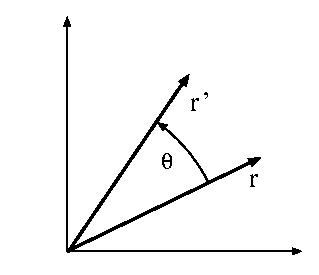
\includegraphics[width=0.8\textwidth]{pics/aktivne}}
\end{minipage}

Ako se ne kaže drukčije, transformacije u ovoj knjizi su "aktivne"
i u tom slučaju
\begin{equation}
\begin{split}
    D(c)& =\left(
\begin{array}{ccc}
\cos(2\pi/3) & -\sin(2\pi/3) & 0 \\
\sin(2\pi/3) & \cos(2\pi/3) & 0 \\
0 & 0 & 1
\end{array}\right) \\
  & =\left(
\begin{array}{ccc}
-1/2 & -\sqrt{3}/2 & 0 \\
\sqrt{3}/2 & -1/2 & 0 \\
0 & 0 & 1
\end{array}\right) \:,
\label{eq:Rc}
\end{split}
\end{equation}
te na kraju
\begin{equation}
D(c^2)=
\left(
\begin{array}{ccc}
-1/2 & \sqrt{3}/2 & 0 \\
-\sqrt{3}/2 & -1/2 & 0 \\
0 & 0 & 1
\end{array}\right) = D(c)^2  \:.
\end{equation}
Lako se provjeri da vrijedi definiciona relacija (\ref{eq:cngp}) grupe
$D(c)^3 = 1$.
\end{primjer}

Ovo naravno nije jedina moguća reprezentacija grupe $\mathrm{C}_3$.
Mogli smo uzeti rotacije za iste kuteve oko bilo koje druge osi i
tako dobiti beskonačno drugačijih reprezentacija.

\begin{primjer}[Reprezentacija grupe C$_3$ na  vektorskom prostoru stanja vodikovog atoma]

Operator koji reprezentira element $c\in\mathrm{C}_3$ će biti
operator $D(c)$ koji transformira valne funkcije vodikovog atoma
\begin{equation}
\psi'(\vec{x})=D(c)\psi(\vec{x}) \:.
\end{equation}
Kako može izgledati takav operator? Strogo uzevši, dovoljno bi bilo pronaći
bilo kakav
operator koji zadovoljava definiciono stvojstvo $D(c)^3 = 1$, ali
pogodno je da to bude upravo operator rotacije za kut 2$\pi$/3.
Neka je $\psi(\vec{x})=\psi_{nlm}(\vec{x})$, dakle gledamo rotaciju
stacionarnih stanja:
\begin{gather}
\psi_{nlm}(\vec{x}) \stackrel{D(c)}{\mapsto}  \psi'_{nlm}(\vec{x}) \\
   \psi'_{nlm}(\vec{x}) = \sum_{n'=1}^{\infty}\sum_{l'=0}^{n'-1}
  \sum_{m'=-l'}^{l'}  D_{(nlm)(n'l'm')}(c)\,  \psi_{n'l'm'}(\vec{x}) \;. 
  \label{eq:nlmexp}
\end{gather}
Ovdje smo iskoristili to da stacionarna stanja čine bazu prostora pa je
transformirano stanje moguće napisati kao linearnu kombinaciju stacionarnih
stanja. Koeficijente $D_{(nlm)(n'l'm')}(c)$ u toj linearnoj kombinaciji
možemo zamisliti kao elemente beskonačnodimenzionalne matrice u beskonačno
dimenzionalnoj bazi čiji su vektori indeksirani trojkom brojeva $(nlm)$, analogno
$3\times 3$ matricama rotacije $D_{(i)(j)}$ u 3D euklidskom prostoru iz prošlog
primjera.

Neka $D(c)$ opet bude rotacija oko $z$-osi.
Rotacija čuva energiju pa se u razvoju (\ref{eq:nlmexp}) mogu pojavljivati 
samo koeficijenti s istim energijskim kvantnim brojem tj. mora biti $n'=n$. 
Na isti način, očuvanje \emph{iznosa} momenta impulsa vodi na $l'=l$. Rotacija
jedino može promijeniti projekciju momenta impulsa $m$ tako da imamo
\begin{displaymath}
D_{(nlm)(n'l'm')}(c)=\delta_{nn'}\delta_{ll'}D^{(l)}_{mm'}(c) \:.
\end{displaymath}
Ovdje je oznaka $(l)$ u $D^{(l)}$ podsjetnik da matrica ovisi o $l$ u najmanju
ruku tako što su njene dimenzije $(2l+1)\times (2l+1)$. Uvrštavanjem ovog u
(\ref{eq:nlmexp}) dobivamo veliko pojednostavljenje
\begin{displaymath}
\psi'_{nlm}(\vec{x})=  \sum_{m'=-l}^{l} D^{(l)}_{mm'}(c) \: \psi_{nlm'}(\vec{x})
\end{displaymath}
tj. relevantna matrica rotacije je konačna.
To je dokud možemo doći u ovom trenutku. U poglavlju \ref{ch:rotacije} ćemo
vidjeti da npr. za $l=1$ i za bilo koji $n$ matrica rotacije ima oblik
\begin{equation*}
D^{(1)}_{mm'}(c)=\delta_{mm'}e^{ -i 2\pi m/3} =
\begin{pmatrix}
e^{-i2\pi/3} & 0 & 0 \\
0 &  1 & 0 \\
0 & 0 & e^{i 2\pi/3}
\end{pmatrix}
\end{equation*}
tj. da rotacija oko $z$-osi ne mijenja niti $m$, što je logično.
Za svaki $l$ imamo drugačiju $(2l+1)$-dimenzionalnu reprezentaciju i
očito ih ima beskonačno mnogo jer $l$ općenito nije ograničen.
\end{primjer}

Oba ova primjera su nas dovela do beskonačnog broja različitih
reprezentacija.
Da bismo uveli red treba nam općenita formalna teorija reprezentacija grupa.


Jedan primjer tvrdnji koje vrijede sasvim općenito je
da svaka grupa $G$ ima tzv. \emph{trivijalnu} reprezentaciju
kod koje je svakom elementu pridružen jedinični operator
\begin{displaymath}
             D(g)=1 \quad \forall g \in G  \;.
\end{displaymath}
Odgovarajući vektorski prostor može biti proizvoljne
dimenzionalnosti pa se čini da i ovih trivijalnih reprezentacija 
ima beskonačno različitih, ali očito je da one nisu različite
na neki zanimljiv i važan način. Formalna teorija reprezentacija
će nam omogućiti da smatramo različitima samo reprezentacije koje
su različite na "zanimljiv" način.

Za zagrijavanje, uvjerimo se u istinitost još jedne općenite tvrdnje,
koja vrijedi za jednodimenzionalne reprezentacije.
One su posebno jednostavne jer
 kompozicija operatora (množenje matrica) postaje obično množenje
 brojeva.
Za konačne grupe sve jednodimenzionalne reprezentacije imaju svojstvo $|D(g)|=1$
za svaki $g \in G$.
Naime, zbog konačnosti grupe, red $n$ svakog elementa 
(vidi Zadatak \ref{zad:redel}) je konačan. Svojstvo homomorfizma
reprezentacije onda povlači da iz $g^n=e$ slijedi $D(g^n)=
  D(g)^n=D(e)=1$, odnosno broj $D(g)$ je $n$-ti korijen jedinice pa može
  biti samo
\begin{equation*}
 D(g)= e^{i 2\pi k/n} \quad k\in\{0,1,\ldots, n-1\} \imp |D(g)|=1 \:.
\end{equation*}

\section{Ekvivalentne reprezentacije}

Vidjeli smo kako element $c \in \mathrm{C}_3$ možemo reprezentirati na
euklidskom prostoru matricom rotacije za kut 2$\pi$/3 oko bilo
koje osi i tako dobiti beskonačno mnogo različitih reprezentacija te
grupe. No očito je da su sve te reprezentacije u nekom smislu
ekvivalentne. Na tom tragu je sljedeća definicija.

\begin{definicija}[Ekvivalentne reprezentacije]
Dvije reprezentacije grupe $G$, $\Gamma_{1}=\{D^{(1)}\}$ i $\Gamma_{2}=\{D^{(2)}\}$ su
\emph{ekvivalentne} ako postoji konstantni nesingularni operator
$S$ takav da je
\begin{displaymath}
        D^{(1)}(g) = S D^{(2)}(g) S^{-1} \quad \forall g \in G
\end{displaymath}
\end{definicija}
Ovdje se pod konstantnošću operatora $S$ misli da on ne ovisi o $g$.
Lako se uvjeriti da ovakva definicija uspostavlja relaciju ekvivalencije
u smislu definicije iz fusnote na stranici \pageref{fn:ekviv}.

Pokazat ćemo sada da u slučaju ekvivalentnih reprezentacija jednu
možemo pretvoriti u drugu prelaskom iz jedne u drugu bazu vektorskog
prostora (pa su u tom smislu one "iste"). Uzmimo neki konkretni operator
$D:V \to V$ iz jedne reprezentacije, koji djeluje na vektorskom prostoru
$V$ i općenito transformira vektore
\begin{equation}
D:\vec{u}\mapsto \vec{v}
\end{equation}
Uzmimo neku bazu $\{\vec{e}_1, \vec{e}_2, \ldots, \vec{e}_n\}\quad$ prostora
$V$ i u njoj će vektor $\vec{u}$ imati komponente $u_i$, 
$\vec{u} =  u_i \vec{e}_i$.
Linearni operator $D$ je potpuno definiran svojim djelovanjem na
vektore baze, a to daje i njegove komponente $D_{ij}$ u toj bazi
\begin{equation}
D \vec{e}_j = (\textrm{linearna kombinacija od } \vec{e}_j) = D_{ij}
  \vec{e}_i \:.
\end{equation}
Ovaj operator sad djeluje na proizvoljni vektor kao
  $D\vec{u}=D( u_j \vec{e}_j)= u_j D_{ij} \vec{e}_i$ 
i ako pišemo $D\vec{u}=\vec{v}=v_i \vec{e}_i$, onda je
$v_i = D_{ij} u_j$, ili u matričnom obliku $v=Du$.

Uzmimo sad neku drugu bazu $\{\vec{f}_1, \vec{f}_2, \ldots, \vec{f}_n\}$
istog vektorskog prostora $V$.
Obzirom na tu bazu, operator $D$ ima neke druge komponente, označimo ih
$D'_{ij}$ tako da je
\begin{align}
    D \vec{f}_j& = D'_{ij} \vec{f}_i  \:, \\
    v'_i& = D'_{ij} u'_j \:.
\end{align}
No, i vektori stare baze su vektori pa se mogu izraziti kao linearna
kombinacija vektora nove baze $\vec{e}_i = S_{ji} \vec{f}_j$.
Tako je vektor $\vec{u}=u_i \vec{e}_i = u_i S_{ji} \vec{f}_j$ tj.
njegove komponente u novoj bazi su
$u'_j = u_i S_{ji}$, a isto bi bilo i za vektor $\vec{v}$,  $v'_j = v_i S_{ji}$.
U matričnom obliku $v'=Sv$ ili  $v=S^{-1}v'$.
Tako je na kraju matrično
\begin{equation}
v'=Sv=SDu=SDS^{-1}u' \:,
\end{equation}
odnosno $\imp D'=SDS^{-1}$ i tako vidimo da operator $S$ koji povezuje
ekvivalentne reprezentacije nije ništa drugo nego operator koji povezuje
dvije baze u kojima te reprezentacije izgledaju isto.\qed

Zadatak će nam biti identificirati i klasificirati reprezentacije koji
\emph{nisu} ekvivalentne u ovom smislu. Drugim riječima, cijelu klasu
ekvivalentnih reprezentacija smatrat ćemo jednom te istom reprezentacijom.
Srećom, da bismo odredili jesu li dvije reprezentacije ekvivalentne
nije nužno tražiti transformaciju $S$. Postoje elegantnije metode
poput upotrebe tzv. \emph{karaktera} reprezentacija
(vidi odjeljak \ref{sec:ortogonalnost}).

Uočimo još da kako su jednodimenzionalne reprezentacije zapravo brojevi koji
automatski komutiraju slijedi da su takve reprezentacije ili identične ili
neekvivalentne.


\section{Zbroj i produkt reprezentacija}

\subsection*{Direktni zbroj reprezentacija}

Kvadratnu matricu oblika
\begin{displaymath}
   \left(
   \begin{array}{cccccc}
        A_1 & & & & & \\
        & A_2 & & & &  \\
        & & \cdot & & & \\
        & & &  \cdot  & & \\
        & & & &  \cdot   & \\
        & & & &  & A_n  \\
\end{array}
   \right)
\end{displaymath}
gdje su $A_i$ kvadratne matrice matrice
zovemo \emph{blok-dijagonalna} ili \emph{blok} matrica.

- Produkt dviju matrica iste blok-strukture:
\begin{displaymath}
\!\!\!\!\!\!\!\!\!\!\!\!\!\!\!\!\!\!\!\!\!\!\!\!\!   \left(
   \begin{array}{cccccc}
        A_1 & & & & & \\
        & A_2 & & & &  \\
        & & \cdot & & & \\
        & & &  \cdot  & & \\
        & & & &  \cdot   & \\
        & & & &  & A_n  \\
\end{array}
   \right)
   \left(
   \begin{array}{cccccc}
        B_1 & & & & & \\
        & B_2 & & & &  \\
        & & \cdot & & & \\
        & & &  \cdot  & & \\
        & & & &  \cdot   & \\
        & & & &  & B_n  \\
\end{array}
   \right)  \\
   =\left(
   \begin{array}{cccccc}
        A_1 B_1 & & & & & \\
        & A_2 B_2 & & & &  \\
        & & \cdot & & & \\
        & & &  \cdot  & & \\
        & & & &  \cdot   & \\
        & & & &  & A_n C_n  \\
\end{array}
   \right)
\end{displaymath}
ima istu blok strukturu kao i te matrice.

- Promotrimo sada dvije reprezentacije grupe $G$: $\Gamma_{1}=\{D^{(1)}(g)\}$
  dimenzije $d_1$ i $\Gamma_{2}=\{D^{(2)}(g)\}$ dimenzije $d_2$.
  Tada je skup matrica 
\begin{displaymath}
   \Gamma = \{D(g)\}= \left\{ \left(
   \begin{array}{cc}
     D^{(1)}(g) & 0 \\
       0  & D^{(2)}(g)
\end{array} \right) \right\}
\end{displaymath}
također reprezentacija grupe $G$.

- Dokaz:
\begin{displaymath}
D(g)D(h)=
\left(
   \begin{array}{cc}
     D^{(1)}(g) & 0 \\
       0  & D^{(2)}(g)
\end{array} \right) 
\left(
   \begin{array}{cc}     
     D^{(1)}(h) & 0 \\
       0  & D^{(2)}(h)
\end{array} \right) 
\end{displaymath}
\begin{displaymath}
=\left(
   \begin{array}{cc}     
     D^{(1)}(g)D^{(1)}(h) & 0 \\
       0  & D^{(2)}(g)D^{(2)}(h)
\end{array} \right) 
=\left(
   \begin{array}{cc}     
     D^{(1)}(gh) & 0 \\
       0  & D^{(2)}(gh)
\end{array} \right) 
=D(gh)
\end{displaymath}
zahvaljujući gornjem svojstvu množenja blok matrica i činjenici
da su $\Gamma_1$ i $\Gamma_2$ reprezentacije.

- Rezultirajuću reprezentaciju zovemo \emph{direktni zbroj}
reprezentacija $\Gamma_1$ i $\Gamma_2$ i pišemo
\begin{displaymath}
\Gamma = \Gamma_1 \oplus \Gamma_2
\end{displaymath}

- Dimenzija zbroja je zbroj dimenzija: $d=d_1 + d_2$

- Možemo zbrajati proizvoljan broj reprezentacija:
\begin{displaymath}
\Gamma = \Gamma_1 \oplus \Gamma_2 \oplus \cdots \oplus \Gamma_n
\end{displaymath}

- Vektorski prostor na koji djeluje zbroj reprezentacija je
  $V=V_1 \oplus V_2$ --- prostor razapet vektorima
  $\{e_1, e_2, \ldots, e_m, f_1, f_2, \ldots, f_n\}$ gdje je
  $\{e_1, e_2, \ldots, e_m\}$ jedna baza od $V_1$, a
  $\{f_1, f_2, \ldots, f_n\}$ jedna baza od $V_2$.

- Primjer: $z$-pravac $\oplus$ $xy$-ravnina = 3D euklidski prostor

- Primjer: vektorski prostor stacionarnih vezanih stanja vodikovog
atoma $\psi_{nlm}$ $\oplus$ vektorski prostor dvočestičnog stanja
nevezanog elektrona i protona (cca. produkt dva ravna vala ako
zanemarimo interakciju)

- Vidjet ćemo da su zanimljive one reprezentacije koje se ne mogu
  prikazati kao zbroj manjedimenzionalnih reprezentacija.

\subsection*{Direktni produkt reprezentacija}

\emph{Kroneckerov} ili \emph{direktni produkt} kvadratnih matrica 
$A$ i $B$ je kvadratna matrica $C=A\otimes B$ čije su komponente
\begin{displaymath}
          C_{ij,kl}=A_{ik}B_{jl}
\end{displaymath}

-Npr, neka su $A$ i $B$ dvodimenzionalne matrice
\begin{displaymath}
A=\left( \begin{array}{cc}
    A_{11} & A_{12} \\
    A_{21} & A_{22}
\end{array} \right) \quad
B=\left( \begin{array}{cc}
    B_{11} & B_{12} \\
    B_{21} & B_{22}
\end{array}\right)  
\end{displaymath}
Onda je njihov direktni produkt matrica
\begin{displaymath}
C=A\otimes B= 
A=\left( \begin{array}{cc}
    A_{11} B & A_{12} B \\
    A_{21} B & A_{22} B
\end{array} \right) =
\left(
\begin{array}{cccc}
  A_{11}B_{11} & A_{11}B_{12} & A_{12}B_{11} & A_{12}B_{12} \\
  A_{11}B_{21} & A_{11}B_{22} & A_{12}B_{21} & A_{12}B_{22} \\
  A_{21}B_{11} & A_{21}B_{12} & A_{22}B_{11} & A_{22}B_{12} \\
  A_{21}B_{21} & A_{21}B_{22} & A_{22}B_{21} & A_{22}B_{22} 
\end{array} \right)
\end{displaymath}

- Dimenzija produkta je produkt dimenzija.

- Vrijedi $(A\otimes B)(C\otimes D)=(AC)\otimes(BD)$

- (Dokaz ovoga vidi u \cite{Jones:1998})

- Ako imamo dvije reprezentacije grupe G: $\Gamma_1$ i $\Gamma_2$,
onda je i skup $\Gamma=\Gamma_1 \otimes \Gamma_2 = \{D(g)\}=
\{D^{(1)}(g)\otimes D^{(2)}(g)\}$ također REP od G:

- $D(g)D(h)=(D^{(1)}(g)\otimes D^{(2)}(g))(D^{(1)}(h)\otimes
  D^{(2)}(h)) = (D^{(1)}(g)D^{(1)}(h))\otimes
 (D^{(2)}(g)D^{(2)}(h)) = D^{(1)}(gh)\otimes D^{(2)}(gh) = D(gh)$


- Ako $\Gamma_1$ djeluje na vektorskom prostoru $V_1$ razapetom
vektorima $\{e_1, e_2, \ldots, e_m\}$, a $\Gamma_2$ na vektorskom
prostoru $V_2$ razapetom vektorima $\{f_1, f_2, \ldots, f_n\}$,
onda $\Gamma=\Gamma_1 \otimes \Gamma_2$ djeluje na vektorskom
prostoru $V=V_1 \otimes V_2$ razapetom vektorima
$\{e_{i}\otimes f_{j}, i=1,\ldots, m; j=1,\ldots, n\}$,
dimenzije $d=mn$.

- Npr. u QM ako imamo dva vodikova atoma koja ne djeluju jedan
na drugog (kao u npr. H$_2$ molekuli) njihove će valne funkcije 
biti vektori u dva Hilbertova prostora:
$\psi_{1}(\vec{x})\in \mathcal{H}_1$ i 
$\psi_{2}(\vec{x})\in \mathcal{H}_2$.
Združeni sustav ta dva atoma možemo promatrati kao jedan vektor
$\psi_{1}(\vec{x})\psi_{2}(\vec{x}) \in \mathcal{H}_1
\otimes \mathcal{H}_2$ gdje je baza od ovog direktnog
produkta Hilbertovih prostora razapeta vektorima
$(\psi_{nlm}(\vec{x})\psi_{n'l'm'}(\vec{x}))$.
Ako atomi djeluju jedan na drugog, valna funkcija će biti
$\psi(x_1, x_2) \in \mathcal{H}_1\otimes \mathcal{H}_2$.

\section{Reducibilnost reprezentacija}

\begin{definicija}[Reducibilna REP]
Reprezentacija $\Gamma$ grupe $G$ koja djeluje na vektorskom
prostoru $V$  je \emph{reducibilna} ukoliko postoji netrivijalni
potprostor $V_{1}$ od $V$ koji je invarijantan na $\Gamma$, tj.
\begin{displaymath}
    D(g)V_{1}\subset V_{1} \quad \forall g \in G \;.
\end{displaymath}
\end{definicija}

- Tada u bazi $\{\vec{e}_1, \ldots, \vec{e}_{m+n} \}$, gdje je baza od
$V_1$ $\{\vec{e}_1, \ldots, \vec{e}_{m} \}$, reprezentacija
poprima oblik
\begin{displaymath}
 D(g) = \left(
\begin{array}{cc}
  D^{(1)}(g) & C(g) \\
     0       & D^{(2)}(g) 
\end{array} \right)
\end{displaymath}
gdje je $D^{(1)}(g)$ $m\times m$, $D^{(2)}(g)$ $n\times n$,
a $C(g)$ $m\times n$ matrica, te dim $V=m+n$ i dim $V_1=m$.

- Obratno, ako postoji baza u kojoj reprezentacija poprima
gornji oblik, reprezentacija je reducibilna.

- $\Gamma_1=\{D^{(1)}\}$ i $\Gamma_2=\{D^{(2)}\}$ su također REP
 od $G$.

Dokaz:
\begin{eqnarray*}
D(g)D(h)&=&\left(
\begin{array}{cc}
 D^{(1)}(g) & C(g) \\ 0 & D^{(2)}(g)
\end{array}\right)
\left(
\begin{array}{cc}
 D^{(1)}(h) & C(h) \\ 0 & D^{(2)}(h)
\end{array}\right)  \\
&=& \left(
\begin{array}{cc}
  D^{(1)}(g)D^{(1)}(h) &  D^{(1)}(g)C(h)+C(g)D^{(2)}(h) \\
       0               &   D^{(2)}(g)D^{(2)}(h)  
\end{array} \right) \\
&=& D(gh) \quad \textrm{jer je $\Gamma$ REP}  \\
&=& \left(
\begin{array}{cc}
 D^{(1)}(gh) & C(gh) \\ 0 & D^{(2)}(gh)
\end{array}\right)  
\end{eqnarray*}
Odakle slijedi
\begin{eqnarray*}
D^{(1)}(gh) &=& D^{(1)}(g)D^{(1)}(h) \\
D^{(2)}(gh) &=& D^{(2)}(g)D^{(2)}(h) \\
\end{eqnarray*}
tj. $\Gamma_1$ i $\Gamma_2$ su REPs.

\begin{primjer}[REP C$_3$ na 3D euklidskom prostoru]

\begin{displaymath}
 D(g)= \left( 
\begin{array}{ccc}
 \cos\theta & -\sin\theta & 0 \\
 \sin\theta& \cos\theta & 0 \\
    0 & 0 & 1 
\end{array}
\right) \quad \forall g \in \textrm{C}_3
\end{displaymath}
2D prostor $V_1$ razapet vektorima $\hat{\vec{x}}$ i $\hat{\vec{y}}$
je invarijantan na $\Gamma$ $\imp \Gamma$ je reducibilna.

- Štoviše, $C(g)=0$ u ovom primjeru tj. vektorski prostor je
  rastavljiv na direktnu sumu dva potprostora koja su oba
invarijantna. To nas vodi na pojam potpune reducibilnosti.
\end{primjer}

\begin{definicija}[Potpuno reducibilna REP]
Ako pored $V_1$ postoji i drugi invarijantni potprostor $V_2$ 
tako da je $V=V_1 \oplus V_2$ tada reprezentaciju $\Gamma$
možemo rastaviti na direktni zbroj $\Gamma=\Gamma_1
\oplus \Gamma_2$ i kažemo da je ona \emph{potpuno reducibilna}.
\end{definicija}


\begin{teorem}[Maschke]
Sve reducibilne reprezentacije konačne grupe su i potpuno
reducibilne.
\end{teorem}

Dokaz u dva koraka:\\
1) Svaka REP konačne grupe je ekvivalentna nekoj unitarnoj REP\\
2) Svaka \emph{unitarna} reducibilna REP je potpuno reducibilna


\emph{Korak 1:} Definiramo ``grupni'' skalarni produkt dvaju
vektora iz $V$ na slijedeći način:
\begin{equation*}
\{\vec{x}, \vec{y}\} \equiv \frac{1}{n}\sum_{g\in G} \big( D(g)\vec{x},
 D(g)\vec{y}\big) \;, 
\end{equation*}
gdje je $n$ red grupe G, a $(\;\,,\;)$ uobičajeni skalarni produkt na $V$.
Sumacija ide preko svih elemenata grupe G.
Grupni skalarni produkt $\{\;\,,\;\}$ zadovoljava sve aksiome skalarnog
produkta. (Provjerite!)
Sada vrijedi
\begin{equation*}
\begin{split}
\{D(h)\vec{x}, D(h)\vec{y}\} &\stackrel{\text{(def.)}}{=} \frac{1}{n}\sum_g \big( D(g) D(h) \vec{x},
 D(g) D(h) \vec{y} \big) \\
&\stackrel{\text{($D$ je rep.)}}= \frac{1}{n}\sum_g \big( D(gh)\vec{x} , D(gh)\vec{y} \big) \\
&=  gh\to k\;;\quad \text{teorem o razmještaju}\;;\quad \sum_g \to \sum_k \\
&= \frac{1}{n}\sum_k \big( D(k) \vec{x}, D(k) \vec{y} \big) \\
&= \{\vec{x}, \vec{y}\} 
\end{split}
\end{equation*}

Dakle, operatori $D(g)$ su unitarni obzirom na grupni skalarni produkt
$\{\;\,,\;\}$. No, nas nas zanima unitarnost obzirom na obični
skalarni produkt $(\;\,,\;)$.
Uzmimo sada da je
\begin{align*}
\{\vec{e}_i\} \quad &\text{ortonormirana baza obzirom na} \quad (\;\,,\;) \\
\{\vec{f}_i\} \quad &\text{ortonormirana baza obzirom na} \quad \{\;\,,\;\}
\end{align*}
i $S$ operator koji povezuje baze: $S\vec{e}_i = \vec{f}_i$. Tada je
\begin{equation*}
\begin{split}
\{ S \vec{x}, S \vec{y}\} &= \{ S x_i \vec{e}_i, S y_j \vec{e}_j \} \\
&= x_{i}^* y_{j}\underbrace{ \{\vec{f}_i, \vec{f}_j\}}_{=\delta_{ij} =
 (\vec{e}_i, \vec{e_j})} \\
&= (x_i \vec{e}_i, y_j \vec{e}_j) \\
&= (\vec{x}, \vec{y})
\end{split}
\end{equation*}
tj. $S$ povezuje grupni i obični skalarni produkt. Ako sada pomoću
ovog operatora $S$ definiramo
ekvivalentnu reprezentaciju $U(g)\equiv S^{-1}DS$ imamo
\begin{equation*}
\begin{split}
\big( U(g)\vec{x}, U(g)\vec{y}\big) &=
\big( S^{-1}D(g)S \vec{x}, S^{-1}D(g)S \vec{y}\big) \\
&= \{ D(g) S \vec{x}, D(g) S \vec{y} \} 
 \qquad \text{\small[$S$ povezuje skalarne produkte]}\\
&= \{ S \vec{x}, S \vec{y} \} \qquad
\text{\small[$D(g)$ je unitaran obzirom na grupni skalarni produkt]}\\
&= (\vec{x}, \vec{y}) \qquad \text{\small[$S$ povezuje skalarne produkte]}
\end{split}
\end{equation*}
Dakle $U(g)$ je unitarna reprezentacija.

\emph{Korak 2:} Treba pokazati da je reducibilna unitarna reprezentacija
uvijek potpuno reducibilna. Ako je $U(g)$ reducibilna to znači da postoji
$V_1$ takav da 
$\forall\vec{x} \in V_1$ i $\forall g\;  U(g) \vec{x} \in V_1 $.

Izaberimo sada ortonormiranu bazu $\{\vec{e}_i\}$ tako da 
$\{\vec{e}_i, i=1,\ldots, n\}$ razapinju $V_1$, a
$\{\vec{e}_i, i=n+1,\ldots, n+m \}$ su preostali vektori koji kompletiraju
bazu od $V$. Vektori $\{\vec{e}_i, i=n+1,\ldots, n+m \}$ razapinju $V_2$ ---
ortogonalni komplement od $V_1$. 

Da bi se pokazala potpuna reducibilnost
reprezentacije $U(g)$ treba pokazati da  je i $V_2$ invarijantan na djelovanje
reprezentacije tj. da 
$\forall\vec{y} \in V_2$ i $\forall g$ vrijedi $U(g) \vec{y} \in V_2$.

Zbog unitarnosti $U(g)$ vrijedi $(U(g) \vec{y} , U(g)\vec{x}) = 
(\vec{y}, \vec{x})$,
za sve $\vec{x}$ i $\vec{y}$ pa onda i posebno za 
$\vec{x}=U(g)^{-1}\vec{x}'\in V_1$ i
$\vec{y} \in V_2$. Dakle, $(U(g)\vec{y}, \vec{x}')=(\vec{y}, U(g)^{-1}\vec{x}')
=0$ zbog ortogonalnosti $\vec{y}$ i $\vec{x}$.
No zbog invarijantnosti $V_1$ i $\vec{x}'$ je element od $V_1$. Dakle iz
$(U(g) \vec{y} , \vec{x}') = 0$ i usljed proizvoljnosti $\vec{y}\in V_2$
i $\vec{x}'\in V_1$ slijedi da je i $V_2$ invarijantan. Q.E.D.


- Osim za konačne grupe ovaj teorem vrijedi i za kontinuirane (Lieve) grupe
ako imaju neko od slijedećih svojstava
\begin{itemize}
\item unitarnost (u drugom koraku dokaza nismo koristili konačnost)
\item kompaktnost,  $(1/g)\sum_g \to \int_g dg$
\item povezanost, nekompaktnost i polujednostavnost (cf. \cite[79]{Cornwell:1997})
\end{itemize}


\begin{definicija}[Ireducibilna reprezentacija]
Reprezentacija $\Gamma$ na vektorskom prostoru $V$ je
\emph{ireducibilna} (IRREP) ako $V$ nema invarijantnih potprostora
izuzev $\{0\}$ i samog sebe.
\end{definicija}


- Identifikacija svih mogućih IRREPsa date grupe te rastav
  proizvoljne reprezentacije na direktni zbroj IRREPsa
\begin{displaymath}
  \Gamma = \sum_{i} \oplus\, \Gamma_{i}
\end{displaymath}
  su nam glavni zadaci za slijedeće poglavlje.



\subsection*{Zadaci}

\begin{enumerate}[label=\arabic{chapter}.\arabic*.]

\item Konstruirajte tri različite jednodimenzionalne reprezentacije
grupe C$_3$.

\item Pokažite da je $\Gamma^* = \{ D(g)^* \}$ reprezentacija ako je
                     $\Gamma   = \{ D(g)   \}$ reprezentacija.

\item Zbrajajući dvije 1D reprezentacije od C$_2$:
\begin{equation}
 \Gamma_1 = \{1, 1\} \qquad i \qquad \Gamma_2 = \{1, -1\}
\end{equation}
konstruirajte 2D reprezentaciju od C$_2$.

\item Dvije 2D reprezentacije od od C$_2$ su
\begin{align*}
\Gamma_1 = \left\{
\begin{pmatrix}
 1 & 0 \\ 0 & 1
\end{pmatrix}\;,
\begin{pmatrix}
 1 & 0 \\ 0 & -1
\end{pmatrix}\right\} \\
\Gamma_2 = \left\{
\begin{pmatrix}
 1 & 0 \\ 0 & 1
\end{pmatrix}\;,
\begin{pmatrix}
 0 & 1 \\ 1 & 0
\end{pmatrix}\right\}\;.
\end{align*}
Konstruirajte njihov direktni zbroj i produkt.

\item Pokažite da
\begin{equation*}
 D(c) = 
\begin{pmatrix}
0 & 1 \\
-1 & -1
\end{pmatrix}
\end{equation*}
generira 2D reprezentaciju grupe C$_3$. Pokažite da je ova reprezentacija
ireducibilna nad poljem realnih brojeva.

\item \label{zad:lnred} Uvjerite se da grupa $\mathbb{R}_{+}\backslash \{0\}, \cdot )$
može biti vjerno reprezentirana na 2D vektorskom prostoru reducibilnom
reprezentacijom
\begin{equation*}
\Gamma = \{ D(g) \} = \left\{
\begin{pmatrix}
1 & \ln g  \\
0 & 1
\end{pmatrix}\right\}
\end{equation*}
Pokažite da ova reprezentacija nije potpuno reducibilna.

\item
Pet funkcija $f(x,y)$
\[
    \{x^4, x^3y, x^2y^2, xy^3, y^4\}
\]
čine bazu peterodimenzionalnog vektorskog prostor $V$. Neka je $\Gamma=
\{D(g)\}$
reprezentacija grupe $D_3$ na $V$ definirana uobičajenim transformacijama
dvodimenzionalnih vektora $(x,y)$, kao u (\ref{eq:Rc}). To npr. znači:
\begin{align*}
   D(c): x^3y &\mapsto \bigg(x\cos\frac{2\pi}{3}-y\sin\frac{2\pi}{3}\bigg)^3
\bigg(x\sin\frac{2\pi}{3}+y\cos\frac{2\pi}{3}\bigg) \\
 &= -\frac{\sqrt{3}}{16} \,  x^{4}  - \frac{1}{2} \, x^{3} y
   - \frac{3\sqrt{3}}{8} \,  x^{2} y^{2} + \frac{3\sqrt{3}}{16} \,  y^{4}
\end{align*}
itd. 
\begin{description}
\item[a)] Odredite matricu $D(b)$ u gornjoj bazi. 
\item[b)] Odredite matricu $D(c)$ u gornjoj bazi.. 
\item[c)] Pokažite da je $\Gamma$ reducibilna tako što ćete identificirati
invarijantni potprostor od $V$.
\end{description}
\secret{
a)
\[
D(b) = \left(\begin{array}{rrrrr}
1 & 0 & 0 & 0 & 0 \\
0 & -1 & 0 & 0 & 0 \\
0 & 0 & 1 & 0 & 0 \\
0 & 0 & 0 & -1 & 0 \\
0 & 0 & 0 & 0 & 1
\end{array}\right)
\]
b)  (Za D.Z.!!)
\[
D(c) =
\left(\begin{array}{ccccc}
\frac{1}{16} & -\frac{1}{16} \, \sqrt{3} & \frac{3}{16} & -\frac{3}{16} \, \sqrt{3} & \frac{9}{16} \\
\frac{1}{4} \, \sqrt{3} & -\frac{1}{2} & \frac{1}{4} \, \sqrt{3} & 0 & -\frac{3}{4} \, \sqrt{3} \\
\frac{9}{8} & -\frac{3}{8} \, \sqrt{3} & -\frac{1}{8} & \frac{3}{8} \, \sqrt{3} & \frac{9}{8} \\
\frac{3}{4} \, \sqrt{3} & 0 & -\frac{1}{4} \, \sqrt{3} & -\frac{1}{2} & -\frac{1}{4} \, \sqrt{3} \\
\frac{9}{16} & \frac{3}{16} \, \sqrt{3} & \frac{3}{16} & \frac{1}{16} \, \sqrt{3} & \frac{1}{16}
\end{array}\right)
\]
c)
$(x^2+y^2)^2$ je invarijanta jer je to kvadrat kvadrata norme vektora u 2D prostoru.
 $\imp a(x^4+2x^2 y^2 +y^4)$ je invarijantni
potprostor 5D prostora.
}

\item Neka je $P$ operator projekcije na potprostor $V_1 \subset V$ (dakle operator sa svojstvima
$P \vec{v} = \vec{v}$ za $\vec{v}\in V_1$ i $P \vec{w} = 0$ za $\vec{w}$ iz ortogonalnog komplementa
od $V_1$ u $V$. Oćito je $P^2 = P$. Pokažite  da je reprezentacija $\Gamma = \{D(g)\}$ 
\begin{itemize}
\item reducibilna ako i samo ako je $PD(g)P = D(g)P$, $\forall g\in G$, te
\item potpuno reducibilna ako i samo ako je $PD(g) = D(g)P$, $\forall g\in G$.
\end{itemize}
Primijenite ovo na zadatak \ref{zad:lnred}.

\end{enumerate}


% Correcting the title chapter page
\fancypagestyle{plain}{%
    \fancyhf{}
    \fancyhead[RO,LE]{\bfseries \thepage}
    \fancyhead[CO]{\rightmark}
    \fancyhead[CE]{\leftmark}
    \renewcommand{\headrulewidth}{0.4pt}}


\chapter{Svojstva ireducibilnih reprezentacija}

\section{Schurove leme}

Sva ključna svojstva ireducibilnih reprezentacija slijede iz 
dvije Schurove leme.

\begin{teorem}[Prva Schurova lema]
Neka operator S povezuje dvije  ireducibilne
reprezentacije $\Gamma=\{D(g)\}$ i $\Gamma'=\{D'(g)\}$ u smislu da je
\begin{displaymath}
  SD(g)=D'(g)S  \quad \forall g\in G  \;.
\end{displaymath}
Tada je ili $S=0$ ili je $S$ invertibilan i imamo
\begin{displaymath}
D(g)=S^{-1}D'(g)S
\end{displaymath}
tj. dvije su reprezentacije ekvivalentne. (Mogućnost
da je $S$ singularan, ali ne i nul-operator je isključena.)
\end{teorem}

\centerline{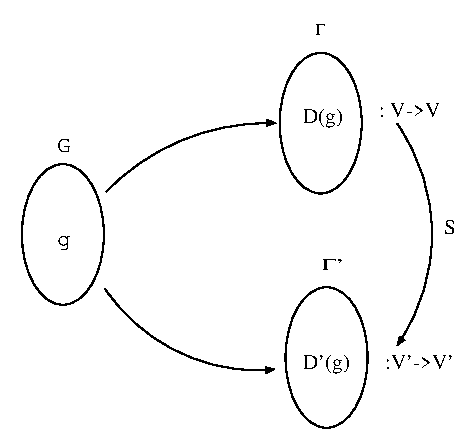
\includegraphics[scale=0.8]{pics/schur.eps}}

\emph{Dokaz.}
Neka su $V$ i $V'$ vektorski prostori na kojima djeluju $\Gamma$ i $\Gamma'$.
Slika $S(V)$ prostora $V$, $S(V)=\{S\vec{x} \td x \in V \}$, je potprostor od $V'$. 
Sva potrebna svojstva
$S(V)$ nasljeđuje od $V'$, a zatvorenost i egzistencija inverza su 
posljedice linearnosti operatora $S$.
Dodatno, $S(V)$ je \emph{invarijantni} potprostor od $V'$ jer
$$D'(g)S\vec{x}=SD(g)\vec{x} \in S(V)\,.$$

Kako je $\{D'(g)\}$ ireducibilna, iz
definicije ireducibilnosti \ref{def:irrep} slijedi
da je ili $S(V)=\{\vec{0'}\}$ ili $S(V)=V'$.

\begin{enumerate}
\item Ako je $S(V)=\{\vec{0'}\}$ tj. svi vektori domene operatora $S$
    preslikavaju se u nul-vektor, to znači da je $S$ nul-operator,  $S=0$.
    To je prva od dvije mogućnosti iz prve Schurove leme.

\item Neka je $S(V)=V'$ tj. $S$ je surjekcija. Promotrimo 
    kernel Ker($S$) koji je zahvaljujući linearnosti od $S$
    potprostor od $V$.
    Uzmimo proizvoljni vektor $\vec{k}$ iz Ker($S$).
    Po pretpostavci leme je 
    $$ S D(g) \vec{k} = D'(g)S\vec{k} = \vec{0'}$$
    što znači da je i $D\vec{k}$ element kernela Ker($S$), odnosno
    i kernel je \emph{invarijantni} potprostor, baš kao i slika.
    Sad, kako je $\{D(g)\}$ ireducibilna slijedi da je ili
    Ker($S$)=$\{\vec{0}\}$ ili Ker($S$)=$V$.
    Ker($S$)$=V$ ne može biti jer onda ne bi bilo $S(V)=V'$ nego bi bilo
      $S(V)=\vec{0'}$.
    Zaključujemo da je Ker($S$)$=\{\vec{0}\}$ pa je $S$ i injekcija (cf.
    teorem \ref{th:izomorfizam} o izomorfizmu) te ima inverz
    i onda iz pretpostavke leme slijedi $D(g)=S^{-1}D'(g)S$, tj.
    dvije su reprezentacije ekvivalentne, što je druga mogućnost leme.\qed 
\end{enumerate}

\begin{teorem}[Druga Schurova lema]
Operator koji komutira sa svim operatorima neke ireducibilne 
reprezentacije
\begin{displaymath}
  D(g)S=SD(g) \quad \forall g\in G
\end{displaymath}
je nužno proporcionalan jediničnom operatoru
(identiteti), $S = \lambda \Eins$.
\end{teorem}

\emph{Dokaz.} Iz fundamentalnog teorema algebre slijedi da $S$ ima
barem jedan svojstveni vektor tj. da postoji
$\vec{x}\neq\vec{0}$ takav da je $S\vec{x}=\lambda\vec{x}$.
To možemo zapisati i u obliku $(S-\lambda\Eins)\vec{x}=0$ što
znači da je $(S-\lambda\Eins)$
singularna matrica (neki vektor $\neq \vec{0}$ preslikava u
$\vec{0'}$ pa nije injekcija).
No, $[S-\lambda\Eins, D(g)]=0$
jer jedinični operator komutira trivijalno, a $S$ komutira po pretpostavci leme.
No onda je po prvoj Schurovoj lemi $S-\lambda\Eins$ nul-operator jer smo upravo vidjeli
da nije regularan. Iz $S-\lambda\Eins=0$ onda odmah slijedi $S=\lambda\Eins$.\qed



\section{Relacije ortogonalnosti i karakteri}
\label{sec:ortogonalnost}

Promotrimo dvije ireducibilne reprezentacije, $\Gamma_{\alpha}$ i $\Gamma_{\beta}$,
koje djeluju na vektorskim prostorima $V^{(\alpha)}$ i $V^{(\beta)}$,
dimenzija $d_\alpha$ i $d_\beta$.
Ako je $\alpha\neq\beta$ podrazumijevat ćemo da su reprezentacije neekvivalentne.
Promotrimo i proizvoljni operator $A$ koji preslikava s $V^{(\beta)}$ na  $V^{(\alpha)}$.
Dakle imamo
\begin{align*}
D^{(\alpha)} &: V^{(\alpha)} \to V^{(\alpha)}\,, \\
D^{(\beta)}  &: V^{(\beta)}  \to V^{(\beta)} \,, \\
A          &: V^{(\beta)} \to V^{(\alpha)} \,.
\end{align*}
Definirajmo sada matricu
\begin{equation*}
B\equiv \sum_{g\in G} D^{(\alpha)}(g) A D^{(\beta)}(g^{-1}) \;.
\end{equation*}
Pokazat ćemo da $B$ zadovoljava pretpostavke Schurovih lema.
Uzimimo proizvoljni element $h\in G$. Tada vrijedi:
\begin{equation*}
\begin{split}
 D^{(\alpha)}(h)B &= \sum_g D^{(\alpha)}(h) D^{(\alpha)}(g) A
    D^{(\beta)}(g^{-1}) \\
&= \sum_g D^{(\alpha)}(hg) A D^{(\beta)}(g^{-1}) \\
&= ( \textrm{zamjenom}\; hg\equiv g' \, , \; g^{-1}=g'^{-1}h ) \\
&= \sum_{g'} D^{(\alpha)}(g') A D^{(\beta)}(g'^{-1}h) \\
&= \sum_{g'} D^{(\alpha)}(g') A D^{(\beta)}(g'^{-1}) D^{(\beta)}(h) \\
&= B D^{(\beta)}(h)
\end{split}
\end{equation*}

U slučaju $\alpha\neq\beta$ ($\Gamma_\alpha$ i $\Gamma_\beta$ nisu 
ekvivalentne),
iz prve Schurove leme slijedi da je $B=0$. Ako je pak $\alpha=\beta$, tj.
$D^{(\alpha)}(h)=D^{(\beta)}(h)$ onda iz druge Schurove leme
slijedi $B=\lambda \Eins$.
Ove se dvije tvrdnje mogu kompaktno ujediniti u relaciju
\begin{equation}
  B = \sum_g D^{(\alpha)}(g) A D^{(\beta)}(g^{-1}) =
 \lambda^{(\alpha)}_A \delta^{\alpha\beta} \Eins \;,
\end{equation}
odnosno, po komponentama,
\begin{equation}
\sum_g D^{(\alpha)}_{ir}(g) A_{rs} D^{(\beta)}_{sl}(g^{-1})
 = \lambda_{A}^{(\alpha)} \delta^{\alpha\beta} \Eins_{il} \,.
 \label{eq:ortpokomp}
\end{equation}
$A$ je ovdje bila proizvoljna matrica. Uzmimo sada konkretnije na mjesto $A$
matricu $A^{(j,k)}$ koja je svugdje nula osim što joj je
element $A^{(j,k)}_{jk}=1$
\begin{displaymath}
 A^{(j,k)}=
\begin{array}{cc}
 & \cdots k \cdots \\
        \begin{array}{c}
         \cdot \\ \cdot \\ j \\ \cdot \\ \cdot \\ \cdot 
        \end{array}
 & 
\begin{pmatrix}
  & \cdot & \\
  & \cdot & \\
 \cdots & 1  & \cdots \\
  & \cdot & \\
  & \cdot & \\
  & \cdot & \\
\end{pmatrix} \,,
\end{array}
\end{displaymath}
\begin{displaymath}
A^{(j,k)}_{rs}=\delta_{rj}\delta_{sk} \,.
\end{displaymath}

Upotrebom te matrice u gornjoj relaciji (\ref{eq:ortpokomp})  dobivamo
\begin{equation}
\sum_g D^{(\alpha)}_{ij}(g) D^{(\beta)}_{kl}(g^{-1}) = 
 \lambda^{(\alpha)}_{jk} \delta^{\alpha\beta} \Eins_{il} \;.
\end{equation}
Sada treba odrediti $\lambda_{jk}$. 
Stavimo ovdje $\alpha =\beta$ i uzmimo trag po $il$ indeksima
množenjem s $\delta_{il}$,
\begin{displaymath}
\sum_g D^{(\alpha)}_{ij}(g) D^{(\alpha)}_{ki}(g^{-1}) = 
 \lambda^{(\alpha)}_{jk} \delta^{\alpha\alpha}\, \textrm{dim}(V^{(\alpha)})
 \equiv \lambda^{(\alpha)}_{jk} d_{\alpha} \,.
\end{displaymath}
S druge strane, to je također jednako
\begin{displaymath}
 \sum_g D(g^{-1}g)_{kj}=\sum_g D(e)_{kj}= \sum_g \Eins_{kj} = \delta_{kj} \sum_g 
 = \delta_{kj} n \;.
\end{displaymath}
Ovdje je $n$ red grupe G.
Slijedi da je
\begin{displaymath}
\lambda^{(\alpha)}_{jk}= \frac{n}{d_{\alpha}}\delta_{kj} \;,
\end{displaymath}
što daje \emph{temeljni teorem o ortogonalnosti} matrica ireducibilnih
reprezentacija:
\begin{teorem}[Ortogonalnost matrica ireducibilnih reprezentacija]
\begin{displaymath}
\sum_g D^{(\alpha)}_{ij}(g) D^{(\beta)}_{kl}(g^{-1}) =
 \frac{n}{d_{\alpha}}\delta^{\alpha\beta}\delta_{il}\delta_{kj} \;.
\end{displaymath}
\label{tm:ortogonalnost}
\end{teorem}

Nadalje, uvijek možemo uzeti da je $D^{(\beta)}(g)$ unitarna matrica
i u tom slučaju je
\begin{displaymath}
\sum_g D^{(\alpha)}_{ij}(g) D^{(\beta)}_{lk}(g)^* =
 \frac{n}{d_{\alpha}}\delta^{\alpha\beta}\delta_{il}\delta_{kj} \;.
\end{displaymath}
Stavimo ovdje $\alpha=\beta$ i promotrimo skup od $d^{2}_\alpha$ vektora
$\vec{x}_{ij}$ iz novog $n$-dimenzionalnog vektorskog prostora,  čije
su komponente dane komponentama svih matrica reprezentacije:
\begin{displaymath}
\vec{x}_{ij} \equiv
(D^{(\alpha)}_{ij}(g_1), D^{(\alpha)}_{ij}(g_2), \ldots, 
D^{(\alpha)}_{ij}(g_n)) \,.
\end{displaymath}
(Ne miješati ovaj
prostor s $V^{\alpha}$ koji je dimenzije $d_\alpha$!) Zbog
\begin{displaymath}
\sum_g D^{(\alpha)}_{ij}(g) D^{(\alpha)}_{lk}(g)^* = (\vec{x}_{lk},\vec{x}_{ij})
 =\frac{n}{d_{\alpha}}\delta_{il}\delta_{kj}
\end{displaymath}
vektori $\vec{x}_{ij}$ su međusobno ortogonalni.
Za neku drugu ireducibilnu reprezentaciju 
$\Gamma_{(\alpha')}$ imamo novih $d_{\alpha'}^{2}$
vektora  koji su ortogonalni međusobno, ali i obzirom na prvih
$d_{\alpha}^{2}$ vektora. Treća ireducibilna reprezentacija daje novih $d_{\alpha''}^{2}$ itd.
No znamo da je općenito maksimalan broj ortogonalnih 
vektora u $n$-dimenzionalnom vektorskom prostoru upravo $n$.
Tako slijedi
\begin{equation}
\sum_{\alpha} d_{\alpha}^{2} \leq n   \,,
\label{eq:sumdlen}
\end{equation}
pa kako je svaka ireducibilna reprezentacija barem jednodimenzionalna
imamo $\sum_{\alpha} d_\alpha \leq n$ tj.
broj ireducibilnih reprezentacija je manji ili jednak broju elemenata grupe.
Štoviše, vrijedi (npr. \cite{Hamermesh:1989}) da je nejednakost
(\ref{eq:sumdlen}) saturirana tj.
\begin{displaymath}
\sum_{\alpha} d_{\alpha}^2 = n \;.
\end{displaymath}
Da bismo odredili broj članova u ovoj relaciji tj.
broj (neekvivalentnih) ireducibilnih reprezentacija grupe, treba nam
pojam \emph{karaktera} reprezentacije.
\begin{definicija}[Karakter reprezentacije]
Karakter $\chi$ reprezentacije $\Gamma=\{D(g)\}$ grupe $G$ je skup
$\chi=\{\chi(g) = \Tr D(g) \td  g\in G\}$.
\end{definicija}
Prvo važno svojstvo je da ekvivalentne reprezentacije imaju iste
karaktere jer zbog cikličnosti traga
imamo $\Tr S D(g) S^{-1} = \Tr D(g)$.
Bez dokaza navedimo da vrijedi i obrat: jednakost karaktera implicira
da su reprezentacije ekvivalentne.
(Usput, taj obrat se \emph{ne} poopćuje na beskonačne kontinuirane grupe, osim
  ukoliko nisu kompaktne, vidi \cite[302]{Cornwell:1997})
Zahvaljujući cikličnosti traga vidimo i da je
$\chi(g)=\Tr D(g) = \Tr D(h) D(g) D^{-1}(h) = \Tr D(hgh^{-1})$
  tj. konjugirani elementi imaju iste karaktere (Oprez: Treba
  razlikovati karakter reprezentacije $\chi$ od njegove komponente
  $\chi(g)$ koju isto često zovemo karakter --- karakter elementa.)

Za unitarnu reprezentaciju vrijedi $\chi(g^{-1}) = \Tr D(g^{-1})= \Tr D^{\dagger}
    = \chi^{*}(g)$.


Uzmimo sada trag po obje matrice
u teoremu o ortogonalnosti \ref{th:ortogonalnost} množenjem
s $\delta_{ij}\delta_{kl}$ pa dobijemo
\begin{displaymath}
\sum_g \chi^{(\alpha)}(g) \chi^{(\beta)}(g)^* = 
\frac{n}{d_{\alpha}} \delta^{\alpha\beta} \delta_{ik}\delta_{ki} =
\frac{n}{d_{\alpha}} \delta^{\alpha\beta} d_{\alpha} =
n \delta^{\alpha\beta} \;.
\end{displaymath}

Definiramo li skalarni produkt karaktera na sljedeći način
 \begin{displaymath}
(\chi, \phi) \equiv \frac{1}{n} \sum_g \chi(g) \phi(g)^* = (\phi, \chi) \;,
\end{displaymath}
imamo
\begin{displaymath}
(\chi^{(\alpha)}, \chi^{(\beta)}) = \delta^{\alpha\beta}
\end{displaymath}
tj. karakteri neekvivalentnih ireducibilnih reprezentacija su ortonormirani
obzirom na taj skalarni produkt.

Neka je sada $k_i$ broj elemenata u $i$-toj klasi konjugacije grupe $G$.
Tada, budući da su karakteri svih elemenata jedne klase konjugacije
isti imamo
\begin{displaymath}
(\chi^{(\alpha)}, \chi^{(\beta)})=\frac{1}{n} \sum_{i=1}^{k}  k_i
 \chi^{(\alpha)}_i \chi^{(\beta)*}_{i} = \delta^{\alpha\beta} \;.
\end{displaymath}
što je iskaz ortogonalnosti vektora u $k$-dimenzionalnom vektorskom
prostoru, gdje je $k$ broj klasa konjugacije grupe. Ortogonalni vektori su
\begin{displaymath}
\vec{\chi}^{(\alpha)} = (\chi^{(\alpha)}_1, \chi^{(\alpha)}_2, \ldots,
 \chi^{(\alpha)}_{k}) \,.
\end{displaymath}
Svaka ireducibilna reprezentacija daje jedan takav $k$-dimenzionalni vektor.
Istim logičkim slijedom kao i ranije ova ortogonalnost vodi na zaključak 
da je broj
ireducibilnih reprezentacija  manji ili jednak broju klasa konjugacije. Štoviše, vrijedi
(vidi literaturu) ortogonalnost vektora:
\begin{displaymath}
\vec{\chi}_i = (\chi^{(\alpha)}_i, \chi^{(\beta)}_i, \ldots)
\end{displaymath}
tj.
\begin{displaymath}
\frac{1}{n} \sum_{\alpha} k_i \chi^{(\alpha)}_i \chi^{(\alpha)*}_j =
\delta_{ij} \,,
\end{displaymath}
što na isti način daje suprotnu nejednakost da je broj klasa konjugacije manji
ili jednak broju ireducibilnih reprezentacija.
Zaključujemo da je broj ireducibilnih reprezentacija grupe 
upravo jednak broju njenih klasa konjugacije!

\section{Tablice karaktera}

\emph{Tablica karaktera} neke grupe je tablica strukture

\begin{tabular}{c|c}
  & Klase konjugacije \\ \hline
\begin{turn}{90} IRREPs \end{turn} & {\Huge $\chi$}
\end{tabular}

Ona često daje dovoljno informacija za praktične primjene, a može
se pomoću slijedećih pravila konstruirati i bez eksplicitnog
poznavanja matrica reprezentacije.

\subsection*{Pravila za konstrukciju tablice karaktera}

\begin{enumerate}

\item Broj ireducibilnih reprezentacija jednak je broju klasa konjugacije 
  grupe. Iz ovoga slijedi da tablica ima jednak broj redova i stupaca. 
  Broj klasa pronalazimo "pješke," analizom grupe.

\item $\sum_{\alpha} d_{\alpha}^2 = n$ često ima jedinstveno rješenje koje
  određuje dimenzionalnosti $d_{\alpha}$ ireducibilnih reprezentacija.

\item Jedinični element grupe je klasa za sebe, a reprezentiran je uvijek
  jediničnom matricom $D^{(\alpha)}(e)=\Eins$ čiji je 
   karakter $\chi^{(\alpha)}(e)=d_{\alpha}$.
  Ovo određuje jedan (konvencionalno prvi) stupac tablice.

\item Uvijek postoji trivijalna jednodimenzionalna ireducibilna
   reprezentacija  $D(g)=\chi(g)=1  \;
    \forall g\in G$.
  Dakle jedan red (konvencionalno prvi) se sastoji od samih jedinica.

\item Za jednodimenzionalne reprezentacije vrijedi $D(g)=\chi(g)$ pa
  sami karakteri reprezentiraju grupu i njihovo množenje mora odražavati
  množenje odgovarajućih elemenata grupe.

\item  \[\sum_{i=1}^{k} k_{i} \chi^{(\alpha)}_{i} \chi^{(\beta) *}_{i} =
    n \delta^{\alpha\beta}\] 
(\emph{Redovi} tablice su ortogonalni i, kad se uzmu u obzir težinski
  faktori $k_i$, normirani su na $n$)

\item  \[\sum_{\alpha=1}^{k} k_{i} \chi^{(\alpha)}_{i} \chi^{(\alpha) *}_{j} =
    n \delta_{ij} \] 
(\emph{Stupci} tablice su ortogonalni i, kad se uzmu u obzir težinski
  faktori $k_i$, normirani su na $n$)

\end{enumerate}

Pravila je najbolje primjenjivati po redu jer su ona s većim rednim
brojem teža za primjenu i rjeđe nužna za kompletiranje tablice.


\begin{primjer}[$D_3$]

Klase konjugacije su (vidi raniji primjer iz odjeljka 1.2):

$K_1=\{e\}$

$K_2 = \{c, c^2\}$

$K_3 = \{ b, bc, bc^2 \}$

1. pravilo $\imp$ 3 IRREPsa

2. $\imp$ $\sum_{\alpha=1}^{3} d_{\alpha}^2 = d_{1}^2 + d_{2}^2
   + d_{3}^2 = n = 6 $ \\
     $\imp d_1 = d_2 =1, d_3=2 $

3. $\imp$ prvi stupac: 1, 1, 2

4. $\imp$ prvi red: 1, 1, 1

\begin{tabular}{c|ccc}
  & $K_1$ & 2$K_2$  & 3$K_3$ \\ \hline
$\Gamma_1$ &   &  &   \\
$\Gamma_2$ &   &  &   \\
 $\Gamma_3$  &   &  &  
\end{tabular}

5. $\chi^{(2)}(b)\chi^{(2)}(c)=\chi^{(2)}(bc), \chi(b)=\chi(bc)$ \\
  $\imp \chi(c)=1$ \\
  $\chi(b)\chi(b)=\chi(b^2)=\chi(e)=1 \imp \chi(b)=\pm 1 $

6. Kad bi bilo $\chi^{(2)}(b)=1$ prva dva reda bi bila jednaka, a ne
   ortogonalna. $\imp \chi^{(2)}(b)=-1$.

   $\sum_{i=1}^{3} k_{i} \chi^{(3)}_{i} \chi^{(1) *}_{i} =
      2+2a+3b=0$ \\
   $\sum_{i=1}^{3} k_{i} \chi^{(3)}_{i} \chi^{(2) *}_{i} =
      2+2a-3b=0$ \\
   $\imp a=-1, b=0$

- obično se za označavanje IRREPsa i klasa koriste kristalografske
   oznake iz priloga.
 

\begin{tabular}{c|ccc}
  & E & 2$C_3$  & 3$C_2$ \\ \hline
$A_1$ & 1 & 1& 1 \\
$A_2$ & 1 & 1&-1 \\
 $E$  & 2 &-1& 0
\end{tabular}

\end{primjer}

\begin{primjer}[$C_3$]

Abelova grupa, svaki element je klasa : $e, c, c^2$

Dakle, tri klase i $d_{1}^2+d_{2}^2+d_{3}^2 = n =3$ pa su
sve tri IRREP 1D.

Prvi red i prvi stupac: sve jedinice

5. pravilo: $\chi(c)^3=\chi(c^3)=\chi(e)=1 \imp \chi(c)=
  \exp(2\pi i k/3), k=0, 1, 2 $

$\chi(c)=1, \omega=e^{2\pi i/3}, \omega^2$

\begin{tabular}{c|ccc}
  & E & $c=C_3$  & $c^2=C_{3}^2$ \\ \hline
$D^{(1)}$ & 1 & 1& 1 \\
$D^{(2)}$ & 1 & $\omega$ &$\omega^2$  \\
 $D^{(3)}$  & 1 &$\omega^2$ & $\omega$ 
\end{tabular}

- provjeriti ortogonalnost

$\omega^2 = \omega^* \imp$ $D^{(2)}$ i $D^{(3)}$ su kompleksno
konjugirane reprezentacije. (Sve smo to već vidjeli ranije u
vježbama.)


Zgodno je uočiti da neabelovska grupa $D_3$ ima i dvodimenzionalnu, dakle matričnu,
ireduciblinu reprezentaciju. To je logično jer neabelovsko svojstvo ne može biti
vjerno reprezentirano jednodimenzionalnim reperezentacijama.
\end{primjer}

\section{Dekompozicija reducibilnih reprezentacija}

Uzmimo neku reprezentaciju $\Gamma$. Po definiciji,
\begin{displaymath}
  \Gamma = \Gamma^{(1)}\oplus\Gamma^{(2)}\oplus\cdots =
     \sum_{\alpha}  a_{\alpha} \Gamma^{\alpha}
\end{displaymath}
gdje su $\Gamma^{\alpha}$ IRREPsi i
gdje je $a_{\alpha}$ \emph{multiplicitet} (broj pojavljivanja) 
IRREPsa $\Gamma^{\alpha}$ u $\Gamma$.


Tr / $ \imp  \chi_i = \sum_{\alpha}  a_{\alpha} \chi^{(\alpha)}_i \quad 
  \forall i$

$\sum_{i=1}^{k} k_i \chi^{(\beta)*}_i /  \imp $

$\sum_{i=1}^{k} k_i \chi_i \chi^{(\beta)*}_i =
\sum_{\alpha}  a_{\alpha} \sum_{i=1}^{k} k_i\chi^{(\alpha)}_i \chi^{(\beta)*}_i
=\sum_{\alpha}  a_{\alpha} n \delta^{\alpha \beta} = n a_{\beta} $


\begin{displaymath}
a_{\alpha} = \frac{1}{n} \sum_{i=1}^{k}  k_i \chi_i \chi^{(\alpha)*}_i
= (\chi^{(\alpha)}, \chi)
\end{displaymath}

\begin{primjer}[REP $\Gamma_V$ od $D_3$ na 3D euklidskom prostoru]
Pod $\Gamma_V$ misli se "vektorska" REP, tj. REP koja djeluje
na pravim 3D vektorima, za razliku od "nepravih" aksijalnih pseudovektora.
$D^{V}(e)=\textrm{diag}(1,1,1)$
\begin{displaymath}
D^{V}(c)=\left(
\begin{array}{ccc}
-1/2 & -\sqrt{3}/2 & 0 \\
\sqrt{3}/2 & -1/2 & 0 \\
0 & 0 & 1
\end{array}\right)
D^{V}(b)=\left(
\begin{array}{ccc}
-1 & 0 & 0 \\
0 & 1 & 0 \\
0 & 0 & -1
\end{array}\right) \textrm{ - rotacija za $\pi$ oko y}
\end{displaymath}
... je reducibilna reprezentacija. Koji je njen rastav na IRREPse?
$\chi=(3,0,-1)$

$a_{A_1} = (\chi, \chi^{(A_1)})=\frac{1}{n}\sum_{i=1}^{3} k_i \chi_i \chi^{(A_1)*}_i
 = \frac{1}{6}(1\cdot 3\cdot 1 + 2\cdot 0\cdot 1 + 3\cdot (-1) \cdot 1)=0$

$a_{A_2} = (\chi, \chi^{(A_2)})
=\frac{1}{6}(1\cdot 3\cdot 1 + 2\cdot 0\cdot 1 + 3\cdot (-1)\cdot(-1))=1$

$a_{E} = (\chi, \chi^{(E)})
=\frac{1}{6}(1\cdot 3\cdot 2 + 2\cdot 0\cdot (-1) + 3\cdot (-1)\cdot 0)=1$

$\Gamma_V  = A_2 \oplus E $

Koji su invarijantni potprostori?

$V^{(A_2)}$ je očito razapet vektorom $\hat{\vec{z}}$, a $\hat{\vec{x}}$ i
$\hat{\vec{y}}$ razapinju 2D potprostor $V^{(E)}$. (Primijetite razliku
prema $C_3$ kod koje je svaki vektor $\vec{v}=a\hat{\vec{z}}$ invarijantan.
$\to$ dipolni momenti.)
\end{primjer}


Direktan zbroj dviju IRREPsa je po definiciji reducibilna REP.
Što je s direktnim produktom?

Pokazali smo ranije da je direktan produkt dviju reprezentacija
$\Gamma^{(1)} \otimes \Gamma^{(2)}$ grupe G također reprezentacija
grupe G. Ona je u općenitom slučaju reducibilna:

\begin{displaymath}
  \Gamma^{(\alpha)}\otimes\Gamma^{(\beta)} =
  \sum \oplus\: a_{\gamma}\Gamma^{(\gamma)} \quad
   \textrm{ - Clebsch-Gordanov razvoj }
\end{displaymath}


Karakter direktnog produkta je produkt karaktera (očito ako pogledamo
matrični izgled direktnog produkta).$\imp$
\begin{displaymath}
a_{\gamma}  = (\chi^{(\gamma)}, \chi^{(\alpha)}\chi^{(\beta)}) \quad
\end{displaymath}

\begin{primjer}[$E\otimes E$ u $D_3$]
$\chi(E)=(2, -1, 0) \imp \chi(E\otimes E)=(4, 1, 0)$

$a_{A_1}=\frac{1}{6}(1\cdot 1\cdot 4+2\cdot 1\cdot 1+3\cdot 1\cdot 0)=1$

$a_{A_2}=\frac{1}{6}(1\cdot 1\cdot 4+2\cdot 1\cdot 1+3\cdot (-1)\cdot 0)=1$

$a_{E}=\frac{1}{6}(1\cdot 2\cdot 4+2\cdot (-1)\cdot 1+3\cdot 0\cdot 0)=1$

$E\otimes E = A_1 \oplus A_2 \oplus E $
\end{primjer}

\section{Primjena: \emph{Dipolni momenti kristala}}

Da bi kristal mogao imati permanentni magnetski ili električni dipolni
moment te veličine moraju biti invarijantne na grupu G simetrije
kristala.

Dipolni momenti su \emph{vektori} 3D euklidskog vektorskog prostora. Slijedi
da je za egzistenciju dipolnih momenata nužno postojanje vektora 
invarijantnih na djelovanje grupe.

Npr. za kristal s $C_3$ simetrijom vektor $\vec{P}$ je invarijantan i
to može biti smjer dipolnog  momenta takvog kristala. $\vec{P}\neq 0$
ne narušava $C_3$ simetriju.

\centerline{
\includegraphics[scale=1.0]{pics/dipol.eps}}

S druge strane, veća $D_3$ simetrija ukida takvu mogućnost. $b$-rotacija
mijenja $\vec{P}\to-\vec{P}$ pa bi $\vec{P}\neq 0$ narušilo simetriju.

\centerline{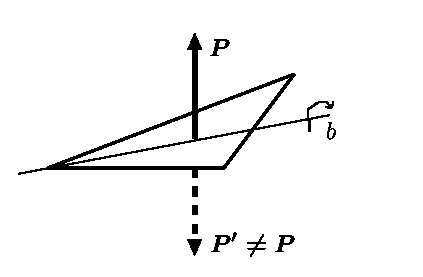
\includegraphics[scale=1.0]{pics/nodipol.eps}}

Simetrični kristal ne može "proizvesti" nesimetrični dipolni moment.

Grupno-teorijski iskaz ovog: \emph{Reprezentacija grupe $G$ na vektorskom
prostoru (potencijalnih) vektora dipolnog momenta mora biti trivijalna tj.
identiteta}:
\begin{displaymath}
   D(g)=1 \quad \forall g\in G \;.
\end{displaymath}
Dakle, da bi kristal mogao imati $\vec{P}\neq 0$, reprezentacija grupe $G$ na 
3D euklidskom vektorskom prostoru mora 
u svojoj dekompoziciji na IRREPse sadržavati identitetu.

Vidjeli smo u prošlom odjeljku da je REP $\Gamma_V$ od $D_3$ na 3D
euklidskom vektorskom prostoru
\begin{displaymath}
             \Gamma_V = A_2 \oplus E \;.
\end{displaymath}
Nema $A_1$ (identitete) $\imp$ nema dipolnog momenta.

S druge strane, za $C_3$ imamo (D.Z.)
\begin{displaymath}
             \Gamma_V = A_1 \oplus E \;.
\end{displaymath}
$\imp$ postoji mogućnost dipolnog momenta.

\textbf{Aksijalni vektori}

Kad grupa pored rotacija sadrži i refleksije ($\sigma$, $S_n$, $i$) treba
uzeti u obzir činjenicu da je magnetski moment $\vec{M}$ aksijalni
vektor (vidi Dodatak \ref{sec:aksijalni})
koji se pri takvim transformacijama ponaša obrnuto od običnog
(polarnog) vektora električnog dipolnog momenta:

\centerline{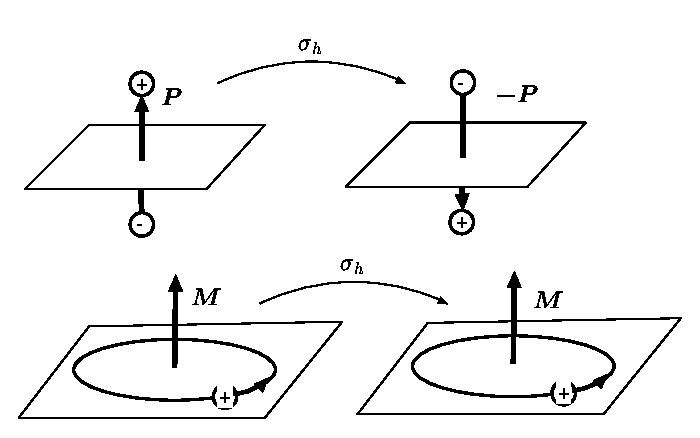
\includegraphics[scale=0.8]{pics/aksijal1.eps}}

\centerline{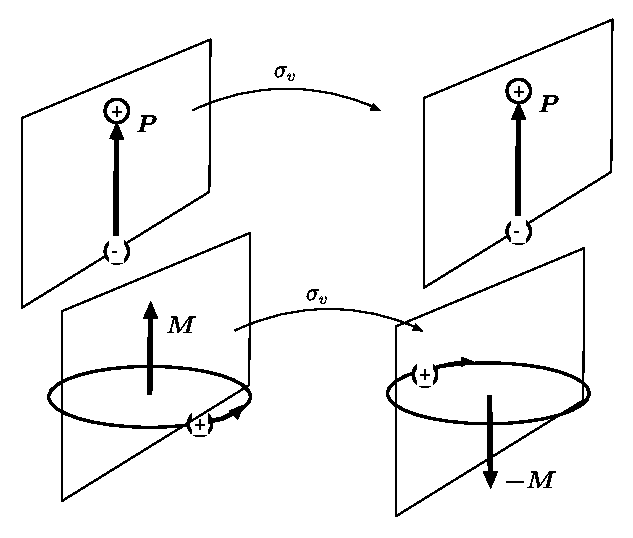
\includegraphics[scale=0.8]{pics/aksijal2.eps}}

(D.Z. Razmislite zašto ogledalo izvrće lijevo-desno, a ne i gore-dolje? kad je
$\sigma_{v_{\mbox{\tiny ogledalo u $x-z$ ravnini}}}:(x, y, z)\to (x, -y, z)$?)

\begin{primjer}[Kristal s $C_{3v}$ simetrijom]

Grupa $C_{3v}$ je izomorfna grupi $D_3$, jedino što $b$ nije rotacija
za $\pi/2$ oko horizontalne osi već refleksija oko vertikalne ravnine
koja sadrži $C_3$ os.

Reprezentacija elemenata $e, c$ i  $c^2$ je kao u primjeru \ref{pr:repC3},
\begin{displaymath}
D(c)=
\left(
\begin{array}{ccc}
-1/2 & -\sqrt{3}/2 & 0 \\
\sqrt{3}/2 & -1/2 & 0 \\
0 & 0 & 1
\end{array}\right) \;, \ldots
\end{displaymath}
s karakterima $\chi^{V}(e)=\mbox{dim}\Gamma_{V}=3$, $\chi^{V}(c)=0$,
a ako osi izberemo kao na slici
\centerline{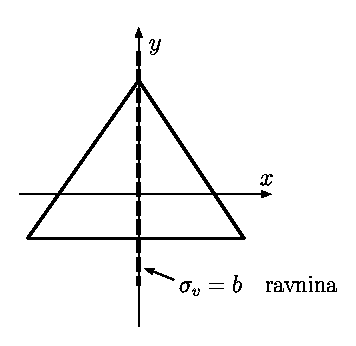
\includegraphics[scale=0.8]{pics/C3vravnina.eps}}
onda je 

\begin{displaymath}
D^{V}(b)=
\left(
\begin{array}{ccc}
-1 & 0 & 0 \\
0 & 1 & 0 \\
0 & 0 & 1
\end{array}\right) 
\end{displaymath}
s karakterom $\chi^{V}(b)=1$.

(Za $D_3$  grupu bi bilo $D^{V}(b)=diag(-1, 1, -1)$, s karakterom
$\chi^{V}(b)=-1$.)

Kako je grupa izomorfna grupi $D_3$ ima istu tablicu karaktera (usput, obrat
ne vrijedi, $Q$ i $T_d$ imaju iste tablice, a nisu izomorfne). Dakle,
imamo:

\begin{tabular}{c|ccc}
  & E & 2$C_3$  & 3$C_2$ \\ \hline
$A_1$ & 1 & 1& 1 \\
$A_2$ & 1 & 1&-1 \\
 $E$  & 2 &-1& 0 \\ \hline
 $\Gamma_V$ & 3 & 0 & 1
\end{tabular}

Iz ovog onda slijedi
\begin{displaymath}
   \Gamma_{V} = A_1  \oplus E
\end{displaymath}

- U rastavu se javlja $A_1$ $\imp$ moguć je permanentni \emph{električni}
 dipolni
moment.


Za aksijalne vektore, reprezentacije elemenata $e, c, c^2$ su iste kao i
gore, ali za $D^{A}(b)$ imamo suprotno od $D^{V}(b)$:

\begin{displaymath}
D^{A}(b)=
\left(
\begin{array}{ccc}
1 & 0 & 0 \\
0 & -1 & 0 \\
0 & 0 & -1
\end{array}\right) 
\end{displaymath}
s karakterom $\chi^{A}(b)=-1$.
(Oblik matrice se može naći i iz razmatranja djelovanja $\sigma_{v}$ na
aksijalni vektor $\vec{c}=\vec{a}\times\vec{b}$ gdje 
su $\vec{a}$ i $\vec{b}$ pravi
vektori: $\sigma_{v}:(a_x, a_y, a_z)\to (-a_x, a_y, a_z)$,
 $\sigma_{v}:(b_x, b_y, b_z)\to (-b_x, b_y, b_z)$
$\imp$  $\sigma_{v}:(c_x, c_y, c_z)\to (c_x, -c_y, -c_z)$.)

Dakle, ukupni karakter je $\chi^{A}=(3, 0, -1)$ odnosno
\begin{displaymath}
      \Gamma_{A} = A_2 \oplus E
\end{displaymath}

Tu nema identitete $A_1$ pa ne može biti ni permanetnog \emph{magnetskog}
dipolnog momenta.
\end{primjer}

\section{Primjena: \emph{Degeneracija i cijepanje energijskih nivoa}}
\label{degeneracija}

Transformacije u kvantnoj mehanici:
\begin{align*}
 \psi' &= U \psi \qquad &\text{za stanja --- vektore} \\
   A' &= U^{-1} A U \qquad &\text{za operatore}
\end{align*}
$U$ --- operator transformacije. Kvantnomehanički sustav, zadan
hamiltonijanom $H_0$, je \emph{simetričan} obzirom na skup transformacija
$\{ U(g_1), U(g_2), \ldots, U(g_n)\}$ ako transformacije ne mijenjaju
hamiltonijan (on, možemo reći, putem Schr\"{o}dingerove jednadžbe definira "izgled"
sustava)
\begin{displaymath}
U^{-1}(g) H_{0} U(g) = H_{0} \quad \forall  g \in \{g_1,\ldots, g_n\}\;.
\end{displaymath}
Ekvivalentno, tada $U(g)$ i $H_0$ komutiraju:
\begin{displaymath}
  H_{0}U(g)=U(g)H_0 \quad \forall  g \in \{g_1,\ldots, g_n\} \;.
\end{displaymath}
Skup svih operatora s ovim svojstvom čini grupu (provjerite!) tj.
reprezentaciju grupe $G=\{g_1,\ldots, g_n\}$ na prostoru kvantnomehaničkih 
stanja.

Stanje sustava s dobro definiranom energijom $\psi_n(\vec{x})$ zove se
\emph{stacionarno stanje} i dano je kao rješenje vremenski 
neovisne Schr\"{o}dingerove jednadžbe
\begin{displaymath}
  H_0 \psi_n(\vec{x}) = E_n \psi(\vec{x}) \;.
\end{displaymath}
Energija transformiranih stanja $\psi'_n(\vec{x}) = U(g)\psi_n(\vec{x})$ je
odgovarajuća svojstvena vrijednost hamiltonijana
\begin{displaymath}
  H_0 \psi'_n(\vec{x}) = H_0 U(g)\psi_n(\vec{x}) = U(g) H_0 \psi_n(\vec{x}) =
 U(g) E_n \psi_n(\vec{x}) = E_n \psi'_n(\vec{x}) \;.
\end{displaymath}
Dakle sva stanja $\psi'_n(\vec{x}) = U(g)\psi_n(\vec{x})$, $\forall g$ imaju
istu energiju $E_n$. Pojavu kad više stanja ima istu energiju 
nazivamo \emph{degeneracija}.

Skup stanja $\{U(g)\psi_n(\vec{x}) \,|\, g\in G\}$ dobivenih transformacijama
datog stanja $\psi_n(\vec{x})$ razapinje
potprostor vektorskog prostora svih stanja sustava. On je
po definiciji invarijantan na djelovanje reprezentacije $\{ U(g) \}$.
Također, reprezentacija $\{ U'(g) \}$ dobivena redukcijom reprezentacije
$\{ U(g) \}$ na ovaj potprostor je ireducibilna što slijedi
iz načina na koji smo konstruirali potprostor.
Takav potprostor naziva se \emph{multiplet}\footnote{Često ze izraz
multiplet koristi i za samu bazu ovog potprostora.}.

Dakle, poznavajući sve IRREPse grupe simetrija nekog kvantnomehaničkog
sustava možemo odrediti mogućnosti degeneracije njegovih stanja ---
one su jednake dimenzionalnostima IRREPsa.

\begin{primjer}[oktahedralna grupa O]

- IRREPsi: $\underbrace{A_1, A_2}_{1D}, \underbrace{E}_{2D},
            \underbrace{T_1, T_2}_{3D}$

- $\imp$ očekujemo jedno-, dvo- i trostruko degenerirane nivoe.

\hspace*{2cm}
\rule{3cm}{1pt}\hspace*{-3cm}%
\rule[2pt]{3cm}{1pt}\hspace*{-3cm}%
\rule[4pt]{3cm}{1pt}\hspace{12pt}%
$\psi_{T_1,1}, \psi_{T_1,2}, \psi_{T_1,3}$

\hspace*{2cm}
\rule{3cm}{1pt}\hspace*{12pt}%
$\psi_{A_2}'$

\hspace*{2cm}
\rule{3cm}{1pt}\hspace*{12pt}%
$\psi_{A_1}$

\hspace*{2cm}
\rule{3cm}{1pt}\hspace*{-3cm}%
\rule[2pt]{3cm}{1pt}\hspace*{12pt}%
$\psi_{E,1}, \psi_{E,2}$

\hspace*{2cm}
\rule{3cm}{1pt}\hspace*{12pt}%
$\psi_{A_2}$

$\psi_{A_2}'$ i $\psi_{A_2}$ su linearno neovisne funkcije.
Pronađemo li neki nivo s prevelikom degeneracijom,
npr\\

\hspace*{2cm}
\rule{3cm}{1pt}\hspace*{-3cm}%
\rule[2pt]{3cm}{1pt}\hspace*{-3cm}%
\rule[4pt]{3cm}{1pt}\hspace{12pt}%
$\psi_{E,1}, \psi_{E,2}, \psi_{A_1}$

to gotovo uvijek znači da nismo dobro identificirali grupu simetrija
tj. da sustav ima veću simetriju nego što smo mislili.

\end{primjer}


\begin{primjer}[Vodikov atom]

Stacionarna stanja su $\psi_{nlm}(\vec{x})$. G=SO(3) --- sferna simetrija.
U 6. poglavlju ćemo vidjeti da su multipleti oblika
\begin{displaymath}
   \{ \psi_{nl(-l)}, \psi_{nl(-l+1)}, \ldots, \psi_{nll}\} \qquad 
\text{($2l+1$ stanja)} \;.
\end{displaymath}
$\imp$ očekujemo $(2l+1)$-struko degenerirane nivoe za svaki $l$. No,
znamo da je zapravo degeneracija $n^2$-struka. Svaka ljuska ima $n^2$
stanja energije
\begin{displaymath}
  E_n \propto \frac{1}{n^2} \qquad \text{neovisno o $l$}
\end{displaymath}
``Slučajna'' degeneracija nivoa s različitim $l$. U 6. poglavlju
ćemo vidjeti da je razlog tome 
postojanje veće simetrije SO(4)=SO(3)$\otimes$SO(3).
\end{primjer}

\subsection*{Cijepanje energijskih nivoa}

Zamislimo sada da neka smetnja $V$  promijeni hamiltonijan
\begin{displaymath}
    H_0 \to H = H_0 + V \;,
\end{displaymath}
tako da je ukupni hamiltonijan $H$ invarijantan na manju grupu $H<G$.
(Npr. slabo električno polje u Starkovom efektu mijenja Hamiltonijan
vodikovog atoma tako da mu doda član proprocionalan električnom polju
i od originalne sferne simetrije preostaje samo aksijalna.)

IRREPsi od $G$ nisu nužno i IRREPsi od $H$. Smanjenje broja transformacija
$U(h)$, $h\in H$ može učiniti da neki potprosotri postanu invarijantni
iako nisu bili invarijantni na potpun skup transformacija $U(g)$, $g\in G$.
Tako su neke IRREPs od G reducibilne obzirom na H i nema razloga da 
nivoi koji odgovaraju dotičnim IRREPsima od G ostanu
degenerirani

\centerline{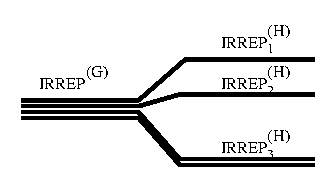
\includegraphics[scale=1.0]{pics/splitting.eps}}
 
Poznavajući dekompoziciju $IRREP^{(G)}$ na $IRREP^{(H)}$
\begin{displaymath}
   IRREP^{(G)}=(\text{reducibilna REP})^{(H)}=
 IRREP^{(H)}_1 \oplus IRREP^{(H)}_2 \oplus \cdots
\end{displaymath}
možemo odrediti strukturu cijepanja. Za određivanje iznosa cijepanja
koriste se metode kvantnomehaničkog računa smetnje.

\begin{primjer}[Cijepanje $T$-nivoa tetrahedralne grupe $T$]

Karakter $T$-nivoa tetrahedralne grupe je
\begin{displaymath}
\begin{tabular}{c|cccc}
  & E & 3$C_2$  & 4$C_3$ & 4$C_{3}'$ \\ \hline
 $T$ & 3  & -1 & 0 & 0 
\end{tabular}
\end{displaymath}

Neka npr. sada kristal doživi fazni prijelaz tako da se
simetrija smanji a) $T\to D_2$ ili b) $T\to C_{3v}$. Pogledajmo
što se događa s gornjim četverostruko degeneriranim nivoom.

a)

\begin{displaymath}
\begin{tabular}{c|cccc}
 & $E$  & $C_{2}^z$ &  $C_{2}^y$ & $C_{2}^x$ \\ \hline
$A_1$ & 1 & 1& 1 & 1 \\
$B_1$ & 1 & 1&-1  & -1\\
$B_2$ & 1 & -1&1  & -1\\
$B_3$ & 1 & -1&-1  & 1\\ \hline \hline
 $T$ & 3 & -1 & -1 & -1
\end{tabular}
\end{displaymath}

Uobičajenim metodama dekompozicije reducibilnih reprezentacija
dobivamo:
\begin{displaymath}
   T = a_1 A_1 \oplus b_1 B_1 \oplus b_2 B_2 \oplus b_3 B_3
\end{displaymath}

\begin{align*}
a_1 &= \frac{1}{n}\sum_k \chi^{(A_1)}(k) \chi^{(T)^*}(k) =
 \frac{1}{4}\big(1\cdot3 + 1\cdot(-1) + 1\cdot(-1) + 1\cdot(-1)\big) = 0 \\
b_1 =b_2 = b_3 &= 1
\end{align*}
\begin{displaymath}
  \imp   T =  B_1 \oplus B_2 \oplus B_3
\end{displaymath}
Dakle degeneracija je potpuno ukinuta

\centerline{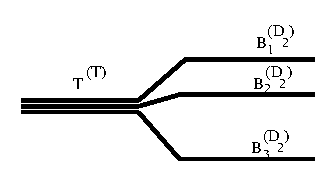
\includegraphics[scale=1.0]{pics/splittingT.eps}}

b) Isti postupak daje
\begin{displaymath}
        T = A_2 \oplus E \;,
\end{displaymath}
tj. degeneracija je samo djelomično ukinuta.

\centerline{\includegraphics[scale=1.0]{pics/splittingT2.eps}}

\end{primjer}

\section{Dodatak: \emph{Kristalografske oznake}}

\textbf{Ireducibilne reprezentacije} $\Gamma^{(\alpha)}$ se obično označavaju
velikim slovima i to tako da se 1D reprezentacije označavaju slovima
$A$ i $B$, 2D reprezentacije slovom $E$, 3D reprezentacije slovom $T$
itd. Par kompleksno konjugiranih 1D reprezentacija se smatra jednom
2D reprezentacijom (jer ih povezuje vremenska inverzija) tako da se
one udružuju vitičastom zagradom i označavaju s $E$.

\textbf{Klase konjugacije} se obično označavaju simbolom $mC_n$ gdje je $m$
broj elemenata klase, a $C_n$ tipični predstavnik klase označen
Sch\"{o}nfliesovim simbolom:

\begin{tabular}{rcl}
$E$ & = & identiteta \\
$C_n$ & = & rotacija za $2\pi/n$ \\
$\sigma$ & = & refleksija preko ravnine \\
$\sigma_{h}$ & = & refleksija preko ``horizontalne'' ravnine tj. ravnine
  okomite da os najveće  \\ && rotacijske simetrije \\
$\sigma_{v}$ & = & refleksija preko ``vertikalne'' ravnine tj. ravnine
  koja sadrži os najveće \\ &&rotacijske simetrije \\
$\sigma_{d}$ & = & refleksija preko ``dijagonalne'' ravnine tj. ravnine
  koja sadrži os najveće \\ && rotacijske simetrije i raspolavlja kut između
  dvije $C_2$ osi okomite na tu os. \\ &&(Specijalni slučaj $\sigma_{v}$.) \\
$S_n$  & = & rotacija za $2\pi/n$ kombinirana s refleksijom preko ravnine
   okomite na \\ && os te rotacije (Ove dvije operacije komutiraju.) \\
$i$ & = &  $S_2 \;\, = \;\,$  inverzija $\vec{r} \to -\vec{r}$
\end{tabular}

\textbf{Točkaste grupe} kristala se označavaju slijedećim
Sch\"{o}nfliesovim oznakama:

\begin{tabular}{rcl}
$C_n$ & = & grupe s jednom $C_n$ osi simetrije \\
$C_{nv}$ & = & grupe s jednom $C_n$ osi i $n$ $\sigma_v$
   refleksijskih ravnina  \\
$C_{nh}$ & = & $C_n$ os,  $\sigma_h$ refleksija $+$ dodaci \\
$S_{n}$ & = & $S_n$ os \\
$D_{n}$ & = & $C_n$ os i $n$ $C_2$ osi okomitih na nju \\
$D_{nd}$ & = & elementi od $D_{n}$ i $\sigma_d$ ravnine refleksije \\
$D_{nh}$ & = & elementi od $D_{n}$ i $\sigma_h$ ravnina refleksije \\
$T$  & = & tetrahedralna grupa \\
$O$  & = & oktahedralna grupa \\
$\cdots$ && $\cdots \quad$ itd. vidi literaturu \\
\end{tabular}

\section{Dodatak: \emph{Aksijalni vektori (pseudovektori)} \label{sec:aksijalni}}
\label{sec:pseudovektori}

\emph{Aksijalni} ili \emph{pseudovektori} su objekti koji se pri rotacijama transformiraju
isto kao i obični (tzv. \emph{polarni}) vektori, ali pri refleksijama i inverzijama
imaju još i dodatnu promjenu predznaka.

Inverzija običnim vektorima u 3D euklidskom prostoru mijenja
predznak $i: \vec{r} \to - \vec{r}$ i može se reprezentirati dijagonalnom
matricom $i = -\Eins = {\rm diag}(-1, -1, -1)$. 

No, vektorski produkt dvaju polarnih vektora, npr. vektora položaja $\vec{r}$
i impulsa $\vec{p}$ posljedično \emph{ne mijenja} predznak:

\[  \vec{L}\equiv \vec{r}\times\vec{p} \; \stackrel{i}{\longrightarrow} \;
  (-\vec{r}) \times (-\vec{p}) =  \vec{r}\times\vec{p} = \vec{L}  \;,
\]

što znači da je $\vec{L}$ (moment impulsa) aksijalni vektor. (U fizici su
veličine koje opisuju rotacije, poput momenta impulsa ili momenta sile, 
često reprezentirane aksijalnim vektorima. Isto vrijedi za veličine
vezane uz magnetizam koji je obično rezultat kruženja (mikro ili makro) struja.)

Da bi se naglasila njihova različitost,
ponegdje u literaturi se aksijalne vektore ne crta kao usmjerene crte
(strelice), već kao crte s ``aksijalnim strelicama'' (cf. 
\cite{Bronstejn:2004} p. 186)

\centerline{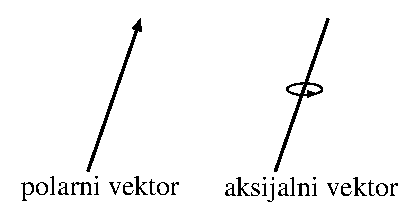
\includegraphics[scale=0.8]{pics/aksijalni_vektor.eps}}

Slično definiramo \emph{pseudoskalarne} veličine kao one koje su skalari
obzirom na rotacije, ali mijenjaju predznak pri refleksijama i inverzijama.
Npr. miješani produkt polarnih vektora je pseudoskalar:

\[
P = (\vec{r}_1 \times \vec{p}) \cdot \vec{r}_2  \; \stackrel{i}{\longrightarrow} \;
  - (\vec{r}_1 \times \vec{p}) \cdot \vec{r}_2 = - P
\]

Magnetski moment, definiran kao $\vec{M} = \frac{1}{2} \int \vec{r}
\otimes \vec{J} dV$ za gustoću struje $J$, odnosno kao
$\vec{M} = \frac{1}{2} q \vec{r} \otimes \vec{v}$ za točkasti
naboj $q$, je dakle aksijalni vektor.

Za još detalja o pseudovektorima i drugim pseudo-veličinama vidi
npr. \cite{Arfken:1995}.

\subsection*{Zadaci}

\begin{enumerate}[label=\arabic{chapter}.\arabic*.]

\item Konstruirajte 2D IRREP grupe $D_3$ koja djeluje na $x-y$ ravnini
i provjerite temeljni teorem o ortogonalnosti.

\item Pokažite da su sve IRREP Abelovih grupa jednodimenzionalne.

\item Pokažite da je nužan i dovoljan uvjet ireducibilnosti reprezentacije
 $\Gamma$ s karakterima $\chi_i$ tzv. Frobeniusov kriterij
\begin{displaymath}
    \sum_i k_i |\chi_i|^2 = n  \;,
\end{displaymath}
gdje je $k_i$ broj elemenata u klasi konjugacije $i$.

\item Konstruirajte tablicu karaktera za grupu $D_4$

\item Pokažite da je direktni produkt dvije 1D IRREP uvijek IRREP.

\item Izrazite reprezentaciju $\Gamma$ grupe $C_{4v}$ koja ima
karaktere
\begin{displaymath}
  \chi(E)=5\;,\quad \chi(C_2)=1\;,\quad \chi(C_4)=-1\;,\quad
  \chi(\sigma_v)=1\;,\quad \chi(\sigma_d)=-3\;,
\end{displaymath}
kao zbroj IRREPsa.
\end{enumerate}


% Correcting the title chapter page
\fancypagestyle{plain}{%
    \fancyhf{}
    \fancyhead[RO,LE]{\bfseries \thepage}
    \fancyhead[CO]{\rightmark}
    \fancyhead[CE]{\leftmark}
    \renewcommand{\headrulewidth}{0.4pt}}

\chapter{Simetrije u klasičnoj i kvantnoj mehanici}
\label{ch:klasicna}

U prošlim poglavljima smo izložili teoriju \emph{konačnih} grupa i njihovih reprezentacija.
Teorija kontinuiranih \emph{beskonačnih} grupa ima svojih posebnosti pa kako
bismo olakšali izlaganje i razumijevanje veza s fizikom, prvo ćemo
prodiskutirati neke općenitije aspekte realizacije simetrija u klasičnoj
i kvantnoj mehanici. Očekuje se da čitaoc vlada osnovama kvantne mehanike,
a kratki podsjetnik dan je u dodatku \ref{sec:qm}.


\section{Transformacije i tenzori}
\label{sec:tenzori}

Vidjeli smo upravo u odjeljcima \ref{sec:dipolni} i \ref{sec:degeneracija} kako
simetrije imaju netrivijalne posljedice na moguća makroskopska
svojstva kristala. U tim primjerima sam fizikalni objekt, kristal, je bio
simetričan tj. isti prije i poslije djelovanja transformacije rotacije.
To i jest uobičajeno laičko razumijevanje značenja riječi \emph{simetrija}. Međutim,
mnoge važne realizacije simetrija u prirodi nisu na razini pojedinih
fizikalnih sustava, nego na razini zakona prirode. Na primjer, zakoni mehanike
i gravitacije su simetrični na sve rotacije, ali Sunčev sustav to nije.
Na rotacije su simetrični i zakoni kvantne mehanike, ali pojedini atomi općenito
nisu.
Svejedno, mnoga svojstva Sunčevog sustava i atoma su diktirana simetrijama
zakona koji tim sustavima upravljaju.
U kasnijim poglavljima ćemo na konkretnim primjerima vidjeti kako se simetrije
prirode odražavaju u konkretnim općenito nesimetričnim sustavima, no
sad ćemo najprije uspostaviti relevantnu terminologiju i pomoću nje još
malo produbiti ovu generičku ideju.


\begin{definicija}[invarijantnost i kovarijantnost]
Fizikalna veličina je \emph{invarijantna} na neku transformaciju ako se
pri toj transformaciji ne mijenja.

Jednadžba koja opisuje fizikalni sustav je \emph{kovarijantna}\footnote{%
Pojmovi kovarijantnosti i kontravarijantnosti
komponenata vektora i tenzora koje srećemo u teoriji relativnosti
("gornji" i "donji" indeksi), a zapravo potječu iz diferencijalne 
geometrije nemaju veze s ovom kovarijantnosti.  To su samo homonimi.}
na neku transformaciju ako se pri toj transformaciji 
njen \emph{oblik} ne mijenja.
\end{definicija}


Tako su na primjer masa ili naboj primjeri veličina invarijantnih na rotacije.
S druge strane, Newtonove jednadžbe za sustav dva tijela koja gravitiraju
\begin{eqnarray}
 m_1 \ddot{\vec{r}}_1 & = & G \frac{m_1 m_2}{|\vec{r}_2 - \vec{r}_1|^3}
    (\vec{r}_2 - \vec{r}_1) \label{eq:newton1} \,, \\
 m_2 \ddot{\vec{r}}_2 & = & G \frac{m_1 m_2}{|\vec{r}_1 - \vec{r}_2|^3}
    (\vec{r}_1 - \vec{r}_2) \,,
\end{eqnarray}
su kovarijantne pri rotacijama. Uvjerimo se u to tako da zarotiramo
sustav za neki kut $\theta$ oko osi usmjerene u smjeru jediničnog vektora $\hat{\vec{n}}$.
Pritom se koordinate položaja prvog tijela mijenjaju kao
\begin{align*}
(\vec{r}_{1})_i \to (\vec{r}_{1}')_i &= \sum_j R_{ij}(\hat{\vec{n}},\theta) 
   (\vec{r}_{1})_j \;, \qquad& \text{(zapis po komponentama)}\\
\vec{r}_{1}\to \vec{r}_{1}' &= R(\hat{\vec{n}},\theta) 
   \vec{r}_{1}\;, \qquad& \text{(matrični zapis)}
\end{align*}
i isto za položaj drugog tijela $\vec{r}_2$.
Ovdje je $R(\hat{\vec{n}},\theta)$ standardna matrica rotacije u trodimenzionalnom
prostoru. Na primjer, za rotaciju oko $z$-osi je
\begin{equation}
R(\hat{\vec{z}},\theta) = \begin{pmatrix}
\cos\theta &  -\sin\theta &  0 \\
\sin\theta &  \cos\theta &  0 \\
    0  &       0     &  1 
\end{pmatrix} \;.
\label{eq:matrot}
\end{equation}
Sada iz (\ref{eq:newton1}) slijedi da je nakon transformacije
jednadžba gibanja za npr. $\vec{r}'_1$ 
\begin{equation}
\begin{split}
m_1 \ddot{\vec{r}}'_1 &= m_1 R \ddot{\vec{r}}_1 \\
   &= G \frac{m_1 m_2}{|\vec{r}_2 - \vec{r}_1|^3}
    (R\vec{r}_2 - R\vec{r}_1) \\
   &= G \frac{m_1 m_2}{|\vec{r}_2 - \vec{r}_1|^3}
    (\vec{r}'_2 - \vec{r}'_1) \\
   &= G \frac{m_1 m_2}{|\vec{r}'_2 - \vec{r}'_1|^3}
    (\vec{r}'_2 - \vec{r}'_1) \;,
\end{split}
\label{eq:kovarijantniNewton}
\end{equation}
i isto za $\vec{r}'_2$, gdje smo radi jednostavnosti prestali
pisati argumente matrice rotacije $R = R(\vec{n},\theta)$
i gdje smo u zadnjem redu iskoristili svojstvo da se iznos
vektora pri rotacijama ne mijenja.
Dakle, jednadžbe zarotiranog sustava imaju isti oblik
(kovarijantne su) premda su konkrentne vektorske veličine
u njima različite tj. $\vec{r}'_{1,2} \neq \vec{r}_{1,2}$.
Drugim riječima, zarotirani sustav poštuje iste zakone kao
i originalni. Trećim riječima, nikakvim eksperimentima stanovnici
drugog zarotiranog sustava ne mogu zaključiti da je sustav zarotiran.
Četvrtim riječima, u prirodi su svi smjerovi ekvivalentni.

Ova i daljnja diskusija podrazumijevaju da govorimo o \emph{aktivnim}
transformacijama koje djeluju na sam fizikalni sustav (vidi
str. \pageref{aktivna}). U \emph{pasivnom}
pristupu u kojem transformiramo samo koordinatni sustav,
ovako napisane jednadžbe su \emph{invarijantne} jer
ako $\vec{r}$ i $\vec{F}$ promatramo kao elemente vektorskog prostora,
a ne kao trojke koordinata tih vektora u nekoj bazi, onda rotacija
koordinatnog sustava ne mijenja same vektore i ono sto je onda
\emph{kovarijantno} je zapis tih jednadžbi po komponentama:
\begin{equation}
       m  \ddot{x}_{i} =  F_{i} \;.
\end{equation}

Kod konstrukcije fizikalnih teorija simetrije prirode će se odražavati
u kovarijantnosti jednadžbi gibanja pa je
važno razviti vještinu prepoznavanja jesu li neke jednadžbe
kovarijantne obzirom na neke transformacije ili nisu. Pogledajmo na primjer
Maxwellove jednadžbe klasične elektrodinamike
\begin{align}
    \nabla \cdot \mathbf{E}  &= \frac{\rho}{\varepsilon_0} \,, \label{eq:maxwell1} \\
\nabla \cdot \mathbf{B}  &= 0 \,, \\
\nabla \times \mathbf{E} &= -\frac{\partial \mathbf{B}}{\partial t}  \,,\\
\nabla \times \mathbf{B} &= \mu_0 \left(\mathbf{J} + 
    \varepsilon_0  \frac{\partial \mathbf{E}}{\partial t} \right) \,. \label{eq:maxwell4}
\end{align}
Gledajući matematičku strukturu članova tih jednadžbi vidimo da je ona
\begin{align*}
    \text{skalar} &= \text{skalar} \,, \\
    \text{skalar} &= \text{skalar}  \,,\\
    \text{vektor} &= \text{vektor}  \,,\\
    \text{vektor} &= \text{vektor} + \text{vektor} \,.
\end{align*}
Zapravo je ovdje riječ o skalarnim i vektorskim \emph{poljima}, dakle veličinama
koje imaju neku skalarnu odnosno vektorsku vrijednost u svakoj točki prostora.
To je pogodan primjer jer su kvantnomehaničke valne funkcije
i kvantna polja, što će nam kasnije biti od velikog interesa, isto polja u tom smislu.

Vidimo da su svi članovi svake pojedine gornje jednadžbe istovrsni i sličnim
razmatranjem kao kod
Newtonovih jednadžbi (\ref{eq:kovarijantniNewton}) lako se uvjeriti da
će jednadžbe zarotiranog
sustava biti istog oblika. Dakle Maxwellove jednadžbe su kovarijantne
na rotacije.
Treba uočiti da za ovakvo razmatranje kovarijantnosti jednadžbi pri rotacijama određujuće svojstvo 
vektora nije to što je on opisan trojkom brojeva niti
to što je on element nekog matematičkog vektorskog prostora već je ključno na koji
se način on transformira pri rotacijama. Skalari se transformiraju trivijalno i
zapravo su invarijantni, dok vektore moramo množiti matricom rotacije:

\vspace*{2ex}
\centerline{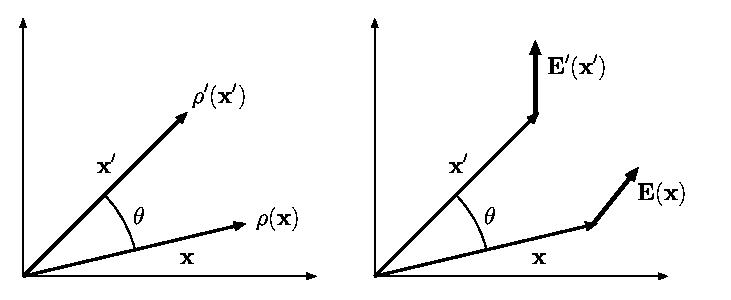
\includegraphics[scale=0.8]{pics/skalarvektor.eps}}

\begin{align*}
    \rho(\vec{r}) &\to \rho'(\vec{r}') = \rho(\vec{r}) \qquad &\textrm{(skalar)} \,, \\
    E_i(\vec{r}) &\to E'_i(\vec{r}') = \sum_j R_{ij}E_j(\vec{r}) 
                 &\textrm{(vektor)} \,,
\end{align*}
gdje je $R_{ij}$ ista matrica (poput (\ref{eq:matrot})) koja rotira
vektor položaja $\vec{r}$. To da se svi vektori rotiraju pomoću identične
matrice je ključno i u ovom kontekstu predstavlja svojevrsnu definiciju
vektora:
\begin{center}
    {vektor} $\equiv$ {objekt koji se pri rotacijama transformira množenjem matricom}
    $R(\hat{\vec{n}}, \theta)$.
\end{center}
Ovo se poopćuje na veličine sa složenijim transformacijskim svojstima,
\emph{tenzore}. 
\begin{definicija}[Tenzor]
\label{def:tenzor}
\emph{Tenzor $n$-tog ranga} (pri rotacijama)  jest veličina $\bbtensor{T}$  koja
se transformira kao
\begin{equation}
 \qquad \bbtensor{T}_{i_1 i_2 \ldots i_n}(\vec{r}) \to \bbtensor{T}'_{i_1 i_2 \ldots i_n}(\vec{r}') =
\sum_{j_1, j_2, \ldots, j_n}
  R_{i_1 j_1}  R_{i_2 j_2} \ldots  R_{i_n j_n} \bbtensor{T}_{j_1 j_2 \ldots j_n}(\vec{r})
 \; . 
 \label{eq:tenzor}
\end{equation}
\end{definicija}

Vidimo da su skalari tenzori nultog, a vektori tenzori prvog ranga.
Komponente tenzora drugog ranga $\bbtensor{T}_{ij}$
možemo po želji prikazati matricom.

\begin{primjer}[Tenzor vodljivosti]
U neizotropnom sredstvu (npr. kristalu), smjer struje $\vec{j}$ ne mora biti isti
kao i smjer narinutog električnog polja $\vec{E}$. U tom slučaju Ohmov zakon
glasi
\begin{equation*}
j_i = \sum_j \sigma_{ij} E_j
\end{equation*}
i uključuje tenzor drugog ranga $\sigma_{ij}$ --- tenzor električne vodljivosti.
\label{pr:tenzorvodljivosti}
\end{primjer}

Tenzorsko svojstvo je vezano uz tip transformacije. Tako postoje
npr. \emph{Lorentzovi tenzori} obzirom na Lorentzove tranformacije
(vidi odjeljak \ref{sec:lorentz}), \emph{izotenzori} obzirom na
izospinske transformacije u subnuklearnoj fizici (vidi odjeljak
\ref{sec:izospin}) i drugi.
Kad se tip transformacije ne specificira obično se misli se na rotacije.

\begin{primjer}[Tenzor elektromagnetskog polja]
 Maxwellove jednadžbe (\ref{eq:maxwell1}--\ref{eq:maxwell4}) su očito
 (nekad se kaže \emph{manifestno}) kovarijantne pri rotacijama kako
 je upravo bilo diskutirano. Einsteinu je za razvoj specijalne teorije relativnosti
 bila centralna kovarijantnost tih jednadžbi i pri Lorentzovim
 transformacijama. I premda Maxwellove jednadžbe jesu kovarijantne
 i pri Lorentzovim transformacijama, ta kovarijantnost
 nije manifestna sve dok se sve veličine ne
 zapišu pomoću Lorentzovih tenzora. Tada se gustoća naboja $\rho$ i
 struje $\vec{j}$ ujedinjuju u četverovektor (Lorentzov tenzor prvog
 ranga) $j^{\mu}$, $\mu=0, 1, 2, 3$, dok se električno i magnetsko
 polje ujedinjuju u Lorentzov tenzor drugog ranga
 $F_{\mu\nu}$ kojeg nazivamo tenzor elektromagnetskog polja ili
  ponekad Faradayjev tenzor. Tada jednadžbe (\ref{eq:maxwell1}) i (\ref{eq:maxwell4})
  možemo zapisati u manifestno kovarijantnom obliku
  \begin{equation}
      \partial_{\mu} F^{\mu\nu} = \mu_0 j^{\nu} \;,
      \label{eq:maxwell4D}
  \end{equation}
  što je eksplicitno pokazano u većini modernih udžbenika 
  elektrodinamike poput \cite{Zangwill:2012}.
\end{primjer}

\begin{primjer}[Riemannov tenzor]
Zakrivljenost $n$-dimenzionalnih ploha se standardno opisuje
tzv. Riemannovim tenzorom $R_{abcd}$  (tenzor četvrtog ranga),
gdje je od posebne važnosti za fiziku Riemannov tenzor prostorvremena
koji ima ključnu ulogu u Einsteinovoj općoj teoriji relativnosti.
\end{primjer}


Da bi jednadžba bila kovarijantna svi njeni članovi se moraju transformirati
na isti način. (Kažemo: moraju se transformirati kovarijantno.)
To znači da moraju pripadati istoj reprezentaciji grupe transformacija.
("Pripadati" u smislu da na svakog djeluje ista reprezentacija. Nisu oni
sami reprezentacije!) Tenzori različitih rangova pripadaju različitim
reprezentacijama. Zanimljivo je pitanje, kojim ćemo se baviti
u poglavlju \ref{ch:rotacije}, jesu li te reprezentacije reducibilne.
 
Kakve su posljedice kovarijantnosti jednadžbi gibanja na njihova
rješenja?
Pojedina rješenja sama za sebe naravno nisu invarijantna, ali 
kovarijantnost jednadžbi gibanja implicira da transformacijom rješenja
dobijemo također dobro rješenje.
Na primjer, sustav dva gravitirajuća tijela s reduciranom koordinatom $\vec{r}
= \vec{r}_1 - \vec{r}_2$ ima kao
rješenje jednadžbi gibanja funkciju $\vec{r}(t)$ koja opisuje elipsu.
Sama ta elipsa nije invarijantna na translacije ili rotacije,
međutim, translatirana elipsa $\vec{r}(t)+\vec{a}$ i zarotirana
elipsa $R\vec{r}(t)$ su isto dobra rješenja za bilo koji $\vec{a}$ i $R$
u što se lako uvjerimo uvrštavanjem u Newtonove jednadžbe.
To da translacijom (rotacijom) rješenja također dobijemo rješenje je posljedica
homogenosti (izotropije) prostora.
Provedemo li unatrag ovaj logički sljed vidimo da homogenost
(izotropija) prostora zahtjeva da jednadžbe gibanja budu kovarijantne
obzirom na translacije (rotacije). Konstrukcija fizikalnih teorija se
često svodi na to da identificiramo sve relevantne simetrije i nakon toga
jednadžbe gibanja slažemo od članova kovarijantnih na sve te simetrije\footnote{%
    U tom su smislu posebno moćne tzv. baždarne simetrije koje u
    određenom smislu vode na jednu jedinstvenu jednadžbu gibanja.
To je omogućilo konstrukciju standardnog modela fizike elementarnih čestica
u drugoj polovici XX. stoljeća koji je još uvijek važeća
teorija svih temeljnih prirodnih sila izuzev gravitacije.}.


\begin{primjer}[Vremenska inverzija]
Promotrimo transformaciju inverzije vremena $t \to -t$.
S jedne strane gornje Newtonove jednadžbe su kovarijantne i obzirom na tu vremensku
inverziju, zahvaljujući tome što je diferencijacija po vremenu koja
se tamo javlja uvijek parnog (drugog) reda. 
I stvarno, vremenski invertirano rješenje dvaju gravitirajućih
tijela u gibanju je također dobro rješenje tj. mogući slučaj u prirodi.
No, kao protuprimjer, vremenska inverzija plina koji slobodno izlazi iz plinske boce nije
moguć događaj što ukazuje na to da priroda nije općenito simetrična na vremensku inverziju i
jednadžbe koje opisuju ekspanziju plina ne bi smjele biti kovarijantne
na takvu inverziju. Neka se čitaoc eskplicitno uvjeri u nekovarijantnost drugog
zakona termodinamike na vremensku inverziju i time će dobiti zadovoljavajuće
razumijevanje ove situacije. Stvarno razumijevanje načina na koji je narušena
ova simetrija u zakonima mehanike čestica plina (dakle ne termodinamike) 
predstavlja zloglasni problem strijele vremena \cite{Zeh:2007}.

\end{primjer}

Za potrebe ove knjige definicija \ref{def:tenzor} daje sve što
je potrebno znati o pojmu tenzora. Dodatak \ref{sec:tenzorKaoStroj} daje
jedan drugačiji pogled koji može pomoći u razumijevanju tog
svepristutnog pojma.


\section{Simetrije i zakoni očuvanja}
\label{sec:noether}

U prošlom smo odjeljku promatrali simetrije Newtonovih klasičnih jednadžbi
gibanja. Ispostavlja se međutim da je
Lagrange-Hamiltonova formulacija klasične mehanike znatno pogodnija od
Newtonove za formalizaciju principa simetrije. Naime, centralni objekt
te formulacije je integral lagranžijana tj. akcija
\begin{equation}
S = \int_{t_0}^{t_1}  L\, dt
    \label{eq:akcija}
\end{equation}
koja je invarijantni skalar obzirom na sve simetrije teorije. Razmatranje
je li akcija invarijantna je znantno lakše od razmatranja jesu li jednadžbe
gibanja kovarijantne. Osim toga, u relativističkoj kvantnoj fizici
(kvantnoj teoriji polja), u skladu s načelima relativistike,
vrijeme prestaje imati posebnu ulogu i jednadžbe gibanja
u vremenu se rijetko koriste. 

No, ostanimo još nakratko u svijetu klasične fizike i podsjetimo se da je jedna
od važnih posljedica simetrija u prirodi postojanje očuvanih veličina.
To je posebno lagano vidjeti u Lagrangeovoj formulaciji kako ćemo sada
vidjeti na primjeru simetrija na prostorne translacije.

Prostorne translacije su transformacije oblika
\begin{equation}
\vec{r}\to\vec{r}'=\vec{r}+\delta\vec{r} \,,
\end{equation}
koje čine grupu $(\mathbb{R}^{3},+)$, no grupnoteorijska svojstva nam ovdje
neće biti bitna, do na činjenicu da ona ima beskonačno elemenata parametriziranih
s tri realna broja. Da bi akcija (\ref{eq:akcija}) bila invarijantna potrebno
je da i sam lagranžijan $L$  bude invarijantan\footnote{Strogo uzevši, akcija
    općenito može biti invarijantna i bez da je lagranžijan invarijantan, no to uključuje
    egzotične efekte na rubovima integracije kakvi se ne javljaju u sustavima
    koje ovdje razmatramo.}, odnosno da je promjena lagranžijana
\begin{equation}
 \delta L = L(\vec{r}', \dot{\vec{r}}', t) -  L(\vec{r}, \dot{\vec{r}}, t)
 =0 \,.
\end{equation}
U infinitezimalnom slučaju, ta je promjena
\begin{equation}
    \delta L =  \sum_{i=1}^{3} \frac{\pd L}{\pd r_i} \delta r_i =0 \;,
\end{equation}
iz čega slijedi da je
\begin{equation}
 \frac{\pd L}{\pd r_i}=0 \,, \quad i=1,2,3 \,,
\end{equation}
jer \emph{homogenost prostora} traži da promjena lagranžijana bude nula
za proizvoljan pomak $\delta r_i$.  Kao posljedica toga, lagranžijan
$L(\vec{r},\dot{\vec{r}},t)=L(\dot{\vec{r}},t)$ ne ovisi eksplicitno
o koordinati $\vec{r}$.
Sada Euler-Lagrangeove jednadžbe gibanja,
\begin{equation}
  \frac{\pd L}{\pd r_i}-\frac{d}{d t} \frac{\pd L}{\pd \dot{r}_i}=0 \,,
\end{equation}
daju zakon očuvanja impulsa
\begin{equation}
\frac{d}{d t} \frac{\pd L}{\pd \dot{r}_i}=
\frac{d}{d t} p_i =0  \;,
\end{equation}
odnosno vektor impulsa $\vec{p}$ je konstanta gibanja.

Na sličan način, homogenost vremena znači invarijantnost lagranžijana
na vremenske translacije (jednoparametarska grupa),
što daje zakon očuvanja energije, a izotropija prostora povlači
invarijantnost lagranžijana na prostorne rotacije (troparametarska
grupa) što daje zakon očuvanja momenta impulsa.
Sve ovo gore su samo posebni primjeri sljedećeg općeg teorema.

\begin{teorem}[Noether]
Ako je sustav invarijantan na $n$-parametarsku
grupu transformacija onda postoji $n$ konstanti gibanja.
\end{teorem}

\section{Transformacije kvantnih sustava}
\label{sec:qmtrans}

Premda su ideje iz odjeljaka \ref{sec:tenzori} i \ref{sec:noether}
jako prisutne i u kvantnoj teoriji, prikazani formalizam nije sasvim
izravno primjenjiv na kvantne sustave. Za razliku od klasičnih sustava
čije stanje je opisano položajima i impulsima čestica (točkom u faznom
prostoru), kvantni sustavi su reprezentirani kao vektor
u odgovarajućem Hilbertovom vektorskom prostoru, a položaj i impuls
su nekomutirajući operatori na tom prostoru. U dodatku \ref{sec:qm}
su rekapitulirane osnove nerelativističke kvantne mehanike, a
nama je posebno važan Wignerov teorem, po kojem su transformacije simetrije
redovito reprezentirane unitarnim i linearnim opearatorima na
Hilbertovom prostoru stanja\footnote{Druga mogućnost je da operatori
    budu antiunitarni i antilinearni, no odgovarajuće transformacije
    uvijek uključuju inverziju vremena čime se nećemo baviti u ovoj knjizi.}.
U ovom odjeljku ćemo upoznati neke operatore transformacija kvantnih
sustava, što će nam poslužiti i kao motivacija za općenitije
proučavanje reprezentacija beskonačnih grupa.

\subsection{Kontinuirane prostorne translacije}
\label{sec:prostornetranslacije}

Poznato je, vidi odjeljak \ref{sec:qm}, da je konkretno kvantno stanje
$|\alpha\rangle$ moguće prikazati u koordinatnoj bazi kao Schr\"{o}dingerovu
valnu funkciju $\psi_{\alpha}(\vec{r}) = \langle \vec{r} | \alpha\rangle$.
Tako eksplicirana ovisnost o prostornoj koordinati $\vec{r}$ će nam
olakšati razmatranje transformacije translacije u prostoru, a za početak
ćemo uzeti da je prostor jednodimenzionalan, $\vec{r} \to x$.
Zanima nas unitarni operator $U_{r}(a)$ koji djelujući na valnu
funkciju sustava $\psi_{\alpha}(x, t)$ daje valnu funkciju 
\begin{equation}
  \psi'_{\alpha}(x,t)= U_{r}(a)\psi_{\alpha}(x,t) \;,
\end{equation}
tog istog sustava, ali translatiranog za udaljenost $a$. (Kao i uvijek,
smatramo da je transformacija aktivna tj. da djeluje na fizikalni,
a ne koordinatni sustav.)

\centerline{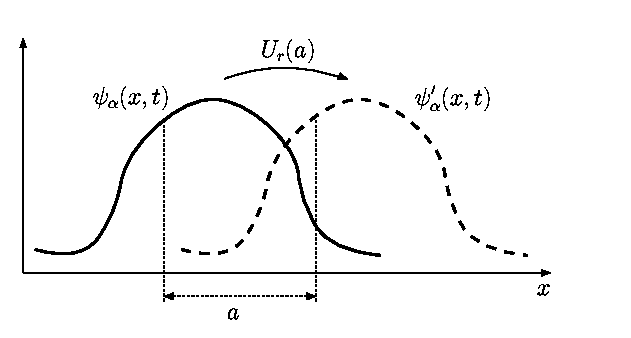
\includegraphics{pics/qmtranslacija.eps}}
Promatrajući crtež, vidimo da vrijedi
\begin{equation}
 \psi'_{\alpha}(x,t)=\psi_{\alpha}(x-a,t) \,,
\end{equation}
odnosno
\begin{equation}
 \psi_{\alpha}(x-a,t)=U_{r}(a)\psi_{\alpha}(x,t)   \,.
 \label{eq:optrans}
\end{equation}
Sada lijevu stranu jednadžbe (\ref{eq:optrans}) razvijemo u Taylorov red
i zbrojimo:
\begin{equation*}
\begin{split}
 \psi_{\alpha}(x-a,t)&=\psi_{\alpha}(x,t)-a\frac{\pd\psi_{\alpha}(x,t)}
{\pd x}+\frac{a^2}{2!}\frac{\pd^2 \psi_{\alpha}(x,t)}{\pd x^2}-\ldots \\
&=\left(1-a\frac{\pd}{\pd x}+\frac{a^2}{2!}\frac{\pd^2}{\pd x^2} - \ldots\right)
\psi_{\alpha}(x,t) \\
&=e^{-a \pd / \pd  x} \psi_{\alpha}(x,t)
\end{split}
\end{equation*}
gdje je eksponencijacija diferencijalnog (ili bilo kakvog drugog) operatora
definirana naznačenom beskonačnom sumom (vidi i dodatak \ref{sec:expmat}).
Usporedbom vidimo da je operator translacije u 1D
\begin{equation}
U_r(a)= e^{-a \pd / \pd  x} \,,
\end{equation}
odnosno, u trodimenzionalnom prostoru ćemo imati
\begin{equation}
U_r(\vec{a})= e^{-\vec{a}\cdot\nabla} \;.
\end{equation}
Poznavajući kvantnomehaničku korespondenciju $-i\hbar\nabla \leftrightarrow
\vec{p}$ imamo konačno općeniti (neovisan o bazi) operator translacije
\begin{equation}
U_r(\vec{a})= e^{-(i/\hbar)\vec{a}\cdot\vec{p}} \;.
\label{eq:Ur}
\end{equation}
Skup translacija čini grupu. Kako svaku translaciju možemo specificirati njenim 
vektorom $\vec{a}$, te kako je kompozicija translacija ekvivalentna zbrajanju
odgovarajućih vektora, vidimo da je ta grupa izomorfna grupi $(\mathbb{R}^3, +)$.

Na malo apstraktniji, ali i općenitiji način, do oblika operatora translacije
možemo doći i razmatranjem koje se ne oslanja na koordinatnu bazu.
Očekivane vrijednosti mjerenja neke veličine koja odgovara hermitskom operatoru $A$
na sustavu u kvantnom stanju $|\alpha\rangle$ 
su dane kao $\langle \alpha | A | \alpha \rangle$ i pri unitarnoj transformaciji $U$
se transformiraju kao 
\begin{equation}
    \langle \alpha | A | \alpha \rangle \to
    \langle U \alpha | A | U \alpha \rangle =
    \langle \alpha | U^{\dagger} A U |  \alpha \rangle =
    \langle \alpha | U^{-1} A U |  \alpha \rangle \;,
\end{equation}
pa transformaciju možemo umjesto na vektorima stanja ekvivalentno promatrati
i na samim operatorima
\begin{equation}
    A \to U^{-1} A U \,.
\end{equation}
Ukoliko nas kao gore zanimaju translacije, očekujemo da se operator položaja
čestice $\vec{x}$ transformira tako da vrijedi
\begin{equation}
    U_{r}(\vec{a})^{-1} \,\vec{x} \, U_{r}(\vec{a}) = \vec{x} + \vec{a} \,.
   \label{eq:defUr}
\end{equation}
Uočite da je plus na desnoj strani ovog izraza konzistentan s definicijom
translacije "udesno" prikazane na gornjoj skici.
Promotrimo sada translaciju za infinitezimalnu udaljenost $\vec{a} \to \vec{\epsilon}$,
$|\vec{\epsilon}| \ll 1$.
Iz razloga kontinuiranosti, odgovarajući operator translacije mora biti
samo infinitezimalno različit od jediničnog operatora pa ga možemo
napisati u obliku
\begin{equation}
    U_{r}(\vec{\epsilon}) = 1 - \frac{i}{\hbar} \vec{p}\cdot\vec{\epsilon} + O(\epsilon^2) \;,
    \label{eq:infinitezimalniUr}
\end{equation}
gdje je $\vec{p}$ operator \emph{definiran} ovim relacijama. Uvrštavanjem
(\ref{eq:infinitezimalniUr}) u (\ref{eq:defUr}) i uspoređivanjem članova
linearnih u $\epsilon_i$ zaključujemo da mora vrijediti
\begin{equation}
    [x_i, p_j] = i\hbar \delta_{ij}\,.
    \label{eq:xpkomutacija}
\end{equation}
Također, kako translacije komutiraju, odgovarajući operatori moraju
zadovoljavati $U_{r}(\vec{\epsilon_1}) U_{r}(\vec{\epsilon_2}) =
U_{r}(\vec{\epsilon_2})U_{r}(\vec{\epsilon_1})$,
pa opet uvrštavanjem i usporedbom članova kvadratnih u $\epsilon_i$
dobivamo
\begin{equation}
    [p_i, p_j] = 0 \;.
    \label{eq:ppkomutacija}
\end{equation}
Ta komutativnost operatora nam sad omogućuje da formalno kompozicijom
operatora N infinitezimalnih translacija za $\vec{\epsilon} = \vec{a}/N$ formiramo 
operator konačne translacije za $\vec{a}$ kao\footnote{Da se uvjerite u ovu
    operatorsku jednakost, uvjerite se da ona vrijedi kad lijeva i desna
    strana djeluju na svojstvene vektore operatora $\vec{p}$, a oni
    čine kompletnu bazu prostora što onda povlači i operatorsku jednakost.}
\begin{equation}
    \lim_{N\to\infty} \left(1 - \frac{i}{\hbar} \frac{\vec{p}\cdot\vec{a}}{N} \right)^N
        = e^{-(i/\hbar)\vec{a}\cdot\vec{p}} \;,
\end{equation}
što je upravo operator translacije $U_r(\vec{a})$ iz (\ref{eq:Ur}).
Naglasimo još jednom da je ovdje operator $\vec{p}$ definiran svojom ulogom
u operatoru translacije (kažemo da on \emph{generira} translacije). 
Kasnije nam daljnja razmatranja trebaju pokazati
da je on kvantnomehanički analogon klasičnom impulsu sustava.


\subsection{Vremenske translacije}
\label{sec:vremensketranslacije}

Potpuno analogno translaciji u jednodimenzionalnom prostoru
možemo definirati operator translacije u vremenu $U_{t}(\tau)$
tako da je valna funkcija transformiranog sustava dana kao
\begin{equation}
 \psi'_{\alpha}(x,t) = \psi_{\alpha}(x,t-\tau) = U_{t}(\tau)\psi_{\alpha}(x,t)\,.
\end{equation}
I opet Taylorovim razvojem dobivamo
\begin{equation}
\begin{split}
 \psi_{\alpha}(x,t-\tau)&=\psi_{\alpha}(x,t)-\tau\frac{\pd\psi_{\alpha}(x,t)}
{\pd t}+\ldots \\
&=e^{-\tau \pd / \pd  t} \psi_{\alpha}(x,t) \;,
\end{split}
\end{equation}
te kvantnomehanička korespondencija $i\hbar\pd /\pd t \leftrightarrow H$
daje
\begin{equation}
U_t(\tau)= e^{(i/h)H\tau} \;.
\end{equation}
Ovo vrijedi samo za $H$ konstantan u vremenu, kakav on jest u većini
nama zanimljivih slučajeva (za ostale slučajeve
vidi diskusiju u \cite{Sakurai:2011}, odjeljak 2.1).

Vremenska \emph{translacija} je transformacija koja daje
stanje sustava koji ima isto ponašanje u vremenskom
trenutku $t+\tau$ kao originalni sustav u trenutku $t$. Vremenska
\emph{evolucija} je pak transformacija koja 
daje stanje sustava u trenutku $t+\tau$ djelujući na stanje
tog istog sustava u ranijem trenutku $t$.
Operator vremenske evolucije se može dobiti iz upravo
navedenog, ako primijetimo da je
\begin{equation}
\psi_{\alpha}(x,t-\tau)=e^{(i/h)H\tau}\psi_{\alpha}(x,t)
\end{equation}
pa zamjenom $\tau\equiv t-t'$ imamo 
\begin{equation}
\psi_{\alpha}(x,t')=e^{-(i/h)H(t'-t)}\psi_{\alpha}(x,t)
\end{equation}
Vrijedi dakle
\begin{equation}
U_{\text{evolucija}}(t' -t)=U^{-1}_{\text{translacija}}(t' -t)
=U_{\text{translacija}}(t -t') \;.
\end{equation}

Promotrimo sada operator $A$ takav da je
$[H,A]=0$. Neka je $\psi(x,t)$ svojstveno stanje od $A$ tj.
\begin{equation}
  A\psi(x,t) = a \psi(x,t)
\end{equation}
Tada to isto stanje nakon vremena $(t'-t)$ zadovoljava
\begin{equation}
  A\psi(x,t')= A e^{-(i/h)H(t'-t)} \psi(x,t) =
 e^{-(i/h)H(t'-t)} A \psi(x,t) = a \psi(x,t')
\end{equation}
tj. $A$ je očuvana veličina. Zaključujemo da su
veličine čiji operatori komutiraju s Hamiltonijanom očuvane u vremenu.
Npr. za slobodnu česticu $H=p^2/2m$ i zbog (\ref{eq:ppkomutacija}) imamo
\begin{equation}
   [H,p]=\frac{1}{2m}[p^2,p]=0
\end{equation}
pa je impuls očuvana veličina.



\subsection{Rotacije}

Rotacije u prostoru su transformacije čija nam je važnost
enormna i zbog važnih primjena u fizici kojima je posvećeno
poglavlje \ref{ch:rotacije} i zbog toga što su one paradigmatski
slučaj na kojem se može izložiti većina gradiva teorije kontinuiranih grupa,
kao u poglavlju \ref{ch:lie}.
Konceptualno, unitarni operator $\mathcal{D}(\hat{\vec{n}}, \phi)$
rotacije\footnote{Koristit ćemo
  tradicionalni simbol $\mathcal{D}$ koji dolazi od njemačke
riječi \emph{Drehung} = rotacija.} za kut $\phi$ oko osi $\hat{\vec{n}}$ dobivamo
istim postupkom kao i operatore translacije u prostoru i vremenu,
jedino intrinsična trodimenzionalnost i nekomutativnost rotacija
malo komplicira izvod.

\centerline{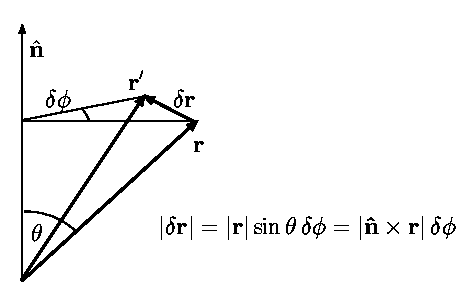
\includegraphics[scale=0.8]{pics/infrotacija.eps}}

Stoga ćemo se odmah usredotočiti na infinitezimalnu rotaciju koja (vidi sliku)
transformira vektor položaja kao
  \begin{equation}
  \vec{r}\to\vec{r}'=\vec{r}+\delta\phi\, \unitn\times\vec{r}  \;.
 \end{equation}
To znači da valna funkcija zarotiranog
sustava treba zadovoljavati
\begin{equation}
\begin{split}
\psi_{\alpha}'(\vec{r}, t)&=\psi_{\alpha}(R(\hat{\vec{n}},\delta \phi)^{-1}
\vec{r}, t) \\
 &=\psi_{\alpha}(\vec{r}-\delta\phi\hat{\vec{n}}\times\vec{r}, t) \\
 &=\psi_{\alpha}(\vec{r}, t)-(\delta\phi\hat{\vec{n}}\times\vec{r})\cdot
  \nabla\psi_{\alpha}(\vec{r}, t) \\
 &= \psi_{\alpha}(\vec{r}, t)-\frac{i}{\hbar}(\delta\phi\hat{\vec{n}}\times
  \vec{r})\cdot \vec{p}\psi_{\alpha}(\vec{r}, t) \\
 &= \left(1-\frac{i}{\hbar}\vec{L}\cdot\hat{\vec{n}}\delta\phi \right)
  \psi_{\alpha}(\vec{r}, t)
\end{split}
\end{equation}

Rotaciju za konačni kut dobijemo kompozicijom N rotacija za $\delta\phi = \phi / N$
gdje $N\to\infty$:

\begin{equation}
\mathcal{D}(\hat{\vec{n}}, \phi)=\lim_{N\to\infty}
\left(1-\frac{i}{\hbar}\vec{L}\cdot\hat{\vec{n}}\delta\phi \right)^N
= e^{-(i/\hbar)\vec{L}\cdot\hat{\vec{n}}\phi}
\label{eq:rotD}
\end{equation}
I opet, ove relacije definiraju operatore $L_i$ kao generatore rotacija,
a kasnija razmatranja pokazuju da je riječ upravo o operatoru koji
odgovara momentu impulsa sustava.
Ukoliko vrijedi $[H,L_{i}]=0$ (a vrijedit će ukoliko neki vanjski utjecaji
ne naruše izotropiju prostora) moment impulsa će biti očuvan.
Poznato je da operatori $L_i$, $i=x,y,z$ zadovoljavaju komutacijske relacije
\begin{equation}
    [L_i, L_j] = i\hbar \epsilon_{ijk}  L_k \,,
    \label{eq:Lkomutacija}
\end{equation}
gdje smo upotrijebili Levi-Civita ili totalno antisimetrični pseudotenzor\footnote{Za
razliku između običnih i pseudotenzora vidi dodatak \ref{sec:aksijalni}.}
trećeg reda definiran
svojim komponentama $\epsilon_{ijk}$ tako da je
\begin{displaymath}
\epsilon_{ijk}=
\begin{cases}
1& \text{ako je $(i,j,k)$ parna permutacija od $(1,2,3)$}, \\
-1& \text{ako je $(i,j,k)$ je neparna permutacija od $(1,2,3)$}, \\
0& \text{inače, tj. ako su dva ili sva tri indeksa ista}.
\end{cases} 
\end{displaymath}
Npr. $\epsilon_{231}=1$, $\epsilon_{213}=-1$, $\epsilon_{221}=0$, itd.

\section{Spin}

U odjeljku \ref{sec:tenzori} vidjeli smo kako veličine u klasičnoj fizici
možemo kategorizirati prema njihovim različitim transformacijskim svojstvima,
recimo na rotacije. Tu smo upoznali tenzore, gdje ovisno o rangu tenzora,
trebamo ga množiti različitim brojem rotacijskih matrica da bismo zapisali
tenzor zarotiranog sustava. Tako očekujemo da i u kvantnoj mehanici jedan
te isti operator
iz (\ref{eq:rotD}) ne može ostvariti
rotaciju proizvoljnog kvantnog sustava.
Uvjerimo se da je to zaista tako
promatrajući rotaciju sustava opisanog vektorskom trojkom valnih funkcija
\begin{equation}
  \vec{\Psi}(\vec{r},t) \equiv (\psi_{x}(\vec{r}, t),
 \psi_{y}(\vec{r}, t), \psi_{z}(\vec{r}, t)) \,.
 \label{eq:psitrojka}
\end{equation}
Takav opis bit će potreban za opis kvantnog stanja čestice za koju nam nije
važan samo njen položaj u prostoru nego i njena orijentacija.
Kao i ranije, tražimo operator $\mathcal{D}(\hat{\vec{n}}, \phi)$, moguće
različit od onog iz (\ref{eq:rotD}), s djelovanjem
\begin{equation}
  \vec{\Psi}'(\vec{r},t) = \mathcal{D}
(\vec{\hat{n}},\phi) \vec{\Psi}(\vec{r},t) \;,
\end{equation}
gdje je $\vec{\Psi}'(\vec{r},t)$ valna funkcija zarotiranog sustava.

\centerline{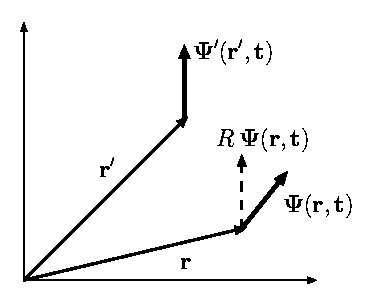
\includegraphics{pics/spin.eps}}

Ukoliko se trojka valnih funkcija iz (\ref{eq:psitrojka}) transformira
pri rotacijama kao standardni vektor, dakle pomoću iste matrice $R(\hat{\vec{n}}, \phi)$
iz odjeljka \ref{sec:tenzori}, iz gornje slike vidimo da zbog promjene
orijentacije čestice treba biti
\begin{gather*}
\vec{\Psi}'(\vec{r}',t)=R \vec{\Psi}(\vec{r},t) \\
\vec{\Psi}'(\vec{r},t)=R \vec{\Psi}(R^{-1}\vec{r},t) 
\end{gather*}
pa imamo, sličnim postupkom kao i ranije
\begin{equation*}
\begin{split}
\mathcal{D}(\vec{\hat{n}},\delta\phi)\vec{\Psi}(\vec{r}, t)&=
 R \vec{\Psi}(R(\hat{\vec{n}},\delta \phi)^{-1}
\vec{r}, t) \\
 &=\vec{\Psi}(R(\hat{\vec{n}}, \delta\phi)^{-1}\vec{r}, t)+
\delta\phi \hat{\vec{n}}\times\vec{\Psi}(
R(\hat{\vec{n}}, \delta\phi)^{-1}\vec{r},t) \\
 &=\vec{\Psi}(\vec{r}-\delta\phi\hat{\vec{n}}\times\vec{r}, t)+
\delta\phi \hat{\vec{n}}\times\vec{\Psi}(\vec{r},t) + O(\delta\phi^2) \\
 &= \vec{\Psi}(\vec{r}, t)-\frac{i}{\hbar}(\delta\phi\hat{\vec{n}}\cdot
  \vec{L})\vec{\Psi}(\vec{r}, t)+
\delta\phi \hat{\vec{n}}\times\vec{\Psi}(\vec{r},t) + O(\delta\phi^2)
\end{split}
\end{equation*}
Vidimo da se obzirom na rotaciju jednokomponentne valne funkcije u prošlom
odjeljku pojavio dodatni član $\delta\phi \hat{\vec{n}}\times\vec{\Psi}(\vec{r},t)$
kojeg ćemo sada zapisati pomoću tripleta matrica $S_{j}$,
definiranih pomoću Levi-Civita pseudotenzora (vidi zadatak \ref{zad:levicivita}):
\begin{equation}
(S_j)_{ik} = i\hbar\epsilon_{ijk} \quad j=1,2,3 \;.
\end{equation}
Konkretno
\begin{align}
S_1& =i\hbar
\begin{pmatrix}
0 & 0 & 0 \\
0 & 0 &-1 \\
0 & 1 & 0
\end{pmatrix} = i\hbar X_1 \,,\\
S_2& = i\hbar
\begin{pmatrix}
0 & 0 & 1 \\
0 & 0 & 0 \\
-1 & 0 & 0
\end{pmatrix} = i\hbar X_2 \,, \\
S_3& = i\hbar
\begin{pmatrix}
0 & -1 & 0 \\
1 & 0 & 0\\
0 & 0 & 0
\end{pmatrix} = i\hbar X_3 \,.
\end{align}
Uz tako definirane matrice imamo
\begin{equation}
\begin{split}
[\hat{\vec{n}}\times\vec{\Psi}]_i &=
\epsilon_{ijk}\hat{n}_j\Psi_k \\
&= -\frac{i}{\hbar}\hat{n}_j (S_j)_{ik}\Psi_k\\
&= -\frac{i}{\hbar}(\hat{\vec{n}}\cdot\vec{S})_{ik}\Psi_k \;,
\end{split}
\end{equation}
što znači
\begin{equation*}
\mathcal{D}(\vec{\hat{n}},\phi)\vec{\Psi}(\vec{r}, t)=
 \left(1-\frac{i}{\hbar}(\vec{L}+\vec{S})\cdot\hat{\vec{n}}\delta\phi \right)
  \Psi(\vec{r}, t) \,,
\end{equation*}
odnosno, operator konačne rotacije ovakvog kvantnog sustava jest
\begin{equation}
\mathcal{D}(\hat{\vec{n}}, \phi)=
 e^{-(i/\hbar)(\vec{L}+\vec{S})\cdot\hat{\vec{n}}\phi} \,.
 \label{eq:rotDJ}
\end{equation}

Hermitske matrice $S_i$ zadovoljavaju iste komutacijske relacije
(\ref{eq:Lkomutacija}) kao i operatori $L_i$ i predstavljaju operatore tzv.
\emph{intrinsičnog}  momenta impulsa poznatog pod nazivom \emph{spin},
za razliku od tzv. \emph{orbitalnog} momenta impulsa kojem odgovaraju
operatori $L_i = (\vec{r}\times\vec{p})_{i}$.
Invarijantnost na rotacije, tj. komutiranje hamiltonijana s operatorom
(\ref{eq:rotDJ}), će onda značiti da je očuvana veličina zapravo
\begin{equation}
\vec{J}=\vec{L}+\vec{S} \,,
\end{equation}
$[H, \vec{J}] = 0$, koju nazivamo \emph{ukupni} moment impulsa, dok je sasvim moguće
da pojedinačno $[H, \vec{L}] \neq 0$ i $[H, \vec{S}] \neq 0$, kao što se na
primjer manifestira u pojavi tzv. vezanja spina i orbite u atomu.
(Elektron usljed orbitiranja "vidi" magnetsko polje
jezgre koje interagira s njegovim magnetskim momentom koji je posljedica
intrinsične vrtnje tj. spina.)

No, ni netom definirani trodimenzionalni operator spina nije najopćenitiji mogući.
U poglavlju \ref{ch:rotacije} vidjet ćemo da ovaj primjer opisuje
vrlo specifičnu situaciju, tzv. česticu spina 1 (točnije $\hbar$),
dok za drugačije iznose intrinsične vrtnje čestica trebamo drugačije
operatore, drugih dimenzionalnosti (npr. spin elektrona koji je iznosa 1/2 
bit će opisan dvodimenzionalnim operatorom).
Za te ćemo potrebe razviti općenitu teoriju
reprezentacija grupe rotacija u kvantnoj mehanici.


\section{Primjena: Blochov teorem}

U ovom ćemo odjeljku pokazati kako primjena teorije grupa elegantno
vodi na važna svojstva valnih funkcija elektrona u kristalu.
\emph{Kristal} je ovdje definiran kao beskonačni trodimenzionalni
sustav atoma koji je invarijantan na translacije 
za bilo koji vektor oblika:
\begin{equation}
  \vec{t}_{\vec{n}} \equiv n_1 \vec{a}_1 + n_2 \vec{a}_2 
  + n_3  \vec{a}_3 \qquad n_{1,2,3}\in\mathbb{Z}\;,
\label{tn}
\end{equation}
gdje su $\vec{a}_{1,2,3}$ tzv. \emph{primitivni vektori} koji definiraju
jediničnu čeliju kristalne rešetke. Prilikom izračuna valne funkcije 
elektronskog
oblaka u kristalu pogodno je zahtijevati da ona zadovoljava tzv.
\emph{Born-von Karmanove periodičke rubne uvjete}:
\begin{equation}
 \psi(\vec{r}) = \psi(\vec{r} + N_1 \vec{a}_1)= \psi(\vec{r} + N_2 \vec{a}_2)
= \psi(\vec{r} + N_3 \vec{a}_3) \;,
\end{equation}
gdje su $N_{1,2,3}$ neki fiksni vrlo veliki ($N_{1,2,3}\gg 1$) prirodni 
brojevi\footnote{
Ovakav zahtjev zamišlja topologiju kristala kao hiper-torusa, što je
dovoljno realistično jer nas ionako topologija ili površinska svojstva
kristala ovdje ne zanimaju, već samo svojstva ``bulk'' materijala poput
specifičnog toplinskog kapaciteta ili električne vodljivosti.
(\emph{Specifični} toplinski kapacitet bakra je naravno isti bez obzira da li je riječ
o ravnoj žici, ploči, beskonačnoj kocki ili pak torusu.)}.

To dalje znači da operatori translacije zadovoljavaju
\begin{equation}
       U_{r}(N_j \vec{a}_j) = U_{r}(0) = 1 \,,  
       \label{eq:Uperiod}
\end{equation}
za svaki $j=1,2,3$ ponaosob (ne sumira se po $j$ u (\ref{eq:Uperiod}),
i odgovarajuća translacijska grupa simetrija ima $N\equiv N_1 N_2 N_3$
elemenata. Kako translacije komutiraju ova grupa je Abelova što
znači da ima $N$ ireducibilnih reprezentacija koje su
sve jednodimenzionalne (cf. npr. Zadatak \ref{zad:1Dabelrep}).
Elementi grupe su generirani translacijom za primitivne vektore
$U_{r}(\vec{a}_j)$  pa tako imamo
\begin{equation}
U_{r}(\vec{a}_1)^{N_1} = 1 
\end{equation}
\begin{equation}
U_{r}(\vec{a}_1) = \exp\Big\{-2\pi i\: \frac{p_1 }{N_1}\Big\} \qquad 
 p_1 \in \{0,1,2,\ldots ,N_1 -1\} \;,
\end{equation}
tj. translacija za $\vec{a}_1$ može biti reprezentirana s
$N_1$ različitih operatora.  Općenita translacija za vektor 
$\vec{t}_{\vec{n}}$ (\ref{tn}) može onda biti reprezentirana jednodimenzionalnim
operatorima oblika
\begin{align}
 U_{r}(\vec{t}_{\vec{n}}) &=
 U_{r}(n_1 \vec{a}_1 + n_2 \vec{a}_2 + n_3  \vec{a}_3) \\
 &= U_{r}(\vec{a}_1)^{n_1} U_{r}(\vec{a}_2)^{n_2} U_{r}(\vec{a}_3)^{n_3} \\
 &= \exp\Big\{ -2\pi i \Big( \frac{n_1 p_1}{N_1} + \frac{n_2 p_2}{N_2} 
 + \frac{n_3 p_3}{N_3} \Big)\Big\} \;,
\label{blochirreps}
\end{align}
tj. s $N$ različitih operatora kako i očekujemo za grupu s $N$ IRREPsa.
Svaka od tih IRREPsa se onda može označiti ("labelirati") s trojkom brojeva $(p_1, p_2, p_3)$
gdje svaki od brojeva $p_j$ može poprimiti bilo koju vrijednost iz
skupa $\{0, 1, 2, \ldots ,N_j -1\}$.
Operator translacije $U_{r}(\vec{t}_{\vec{n}})$ je u konkretnom IRREPsu 
 $(p_1, p_2, p_3)$ reprezentiran operatorom/brojem (\ref{blochirreps}).

Umjesto trojke $(p_1, p_2, p_3)$ za označavanje IRREPsa se obično
upotrebljavaju vektori $\vec{k}$ definirani na slijedeći način. Prvo
definiramo tzv. vektore \emph{recipročne rešetke} $\vec{b}_1, \vec{b}_2,
\vec{b}_3$ putem zahtjeva:
\begin{equation}
   \vec{a}_i\cdot \vec{b}_j = 2 \pi \delta_{ij} \qquad i,j = 1, 2, 3 \;.
\label{defb}
\end{equation}
Sada vektor $\vec{k}$ koji odgovara IRREPsu
$(p_1, p_2, p_3)$ definiramo kao
\begin{equation}
  \vec{k} \equiv \frac{p_1}{N_1}\vec{b}_1 + \frac{p_2}{N_2}\vec{b}_2 + 
  \frac{p_3}{N_3}\vec{b}_3 \;.
\label{defk}
\end{equation}
Iz (\ref{defk}), (\ref{defb}) i (\ref{blochirreps}) slijedi da je
operator translacije za $\vec{t}_{\vec{n}}$ u IRREPsu $\vec{k}$
dan s
\begin{equation}
 U_{r}^{(\vec{k})} (\vec{t}_{\vec{n}}) = 
 e^{-i \vec{k}\cdot \vec{t}_{\vec{n}}} \;,
\end{equation}
i odsad $N$ različitih $\vec{k}$-ova (\ref{defk}) labelira IRREPse.
Vidimo da dimenzija $\vec{k}$ odgovara valnom broju, tj. impulsu
podijeljenom s Planckovom konstantom.

Djelovanje ovih operatora translacije na valne funkcije u datom
IRREPsu mora biti kao i kod svih operatora translacije (\ref{eq:optrans})
\begin{equation}
 e^{-i \vec{k}\cdot \vec{t}_{\vec{n}}} \psi_{\vec{k}}(\vec{r}) =
\psi_{\vec{k}}(\vec{r} - \vec{t}_{\vec{n}}) \;.
\label{bloch}
\end{equation}
Kako je riječ o običnim brojevima (a ne recimo o diferencijalnim
operatorima) dobili smo razmjerno jednostavan uvjet koji valne funkcije
u kristalu moraju zadovoljavati da bi bile svojstvene funkcije operatora
translacije. Takve funkcije se nazivaju \emph{Blochove funkcije}, a
$\vec{k}$ je Blochov valni vektor.
Zašto su one zanimljive?

Kao prvo, ako ih (bez gubitka općenitosti) zapišemo u obliku
\begin{equation}
 \psi_{\vec{k}}(\vec{r}) = e^{+i \vec{k}\cdot \vec{r}} u_{\vec{k}}(\vec{r})
\end{equation}
onda odmah iz (\ref{bloch}) dobijemo uvjet 
\begin{equation}
  u_{\vec{k}}(\vec{r}) = u_{\vec{k}}(\vec{r} - \vec{t}_{\vec{n}})  \;,
\end{equation}
dakle Blochove funkcije su oblika 
$e^{+i \vec{k}\cdot \vec{r}} u_{\vec{k}}(\vec{r})$,
gdje je $u_{\vec{k}}(\vec{r})$ periodička funkcija na rešetci.
S druge strane, operator translacije na rešetci komutira s Hamiltonijanom
\begin{equation}
    [H, U_{r}^{(\vec{k})} (\vec{t}_{\vec{n}}) ] = 0 \;,
\end{equation}
kako i očekujemo od operatora simetrije.
Komutiranje s kinetičkim dijelom je trivijalno jer su i kinetički dio
hamiltonijana i operator translacije funkcije samo impulsa koji
komutiraju međusobno.  Komutiranje s potencijalom je manje trivijalno
i posljedica je periodičnosti $V(\vec{r}) = 
V(\vec{r}+\vec{t}_{\vec{n}})$\footnote{Po analogiji s
    (\ref{eq:defUr}) za svaki operator $A(\vec{r})$ vrijedi
    $U_{r}^{-1}(\vec{t}_{\vec{n}})
A(\vec{r}) U_{r}(\vec{t}_{\vec{n}}) = A(\vec{r}+\vec{t}_{\vec{n}})$,
pa onda to vrijedi i za $A=V$ pa iz toga i iz periodičnosti $V$ odmah slijedi tražena
komutativnost.}.
Posljedica komutiranja dvaju operatora je da oni imaju zajedničke
svojstvene funkcije. To onda povlači
\begin{teorem}[Bloch]
Valne funkcije periodičke rešetke mogu se izabrati kao Blochove funkcije.
\end{teorem}

Ovo onda olakšava rješavanje Schr\"{o}dingerove jednadžbe
za rešetku jer je potrebno naći samo funkcije $u_{\vec{k}}(\vec{r})$ za
svaki $\vec{k}$,
a njihova periodičnost umnogome pojednostavljuje taj zadatak,
kako svjedoče brojni primjeri iz fizike čvrstog stanja.
Blochov teorem se obično izvodi i u udžbenicima fizike čvrstog
stanja, no ovdje smo dali naglasak
na grupno-teorijski pristup tj. korespondenciju s reprezentacijama
grupe translacija.

\subsection*{Zadaci}

\begin{enumerate}[label=\arabic{chapter}.\arabic*.]

\item \label{zad:kronecker} Kroneckerov simbol $\delta_{ij}$, $i,j \in \{1, 2, 3\}$ je tenzor drugog ranga
    obzirom na rotacije. Tenzori su općenito definirani kao veličine 
    \emph{kovarijantne} pri datim transformacijama. Pokažite da je $\delta_{ij}$
    također i \emph{invarijantan}.
\item Pokažite da je operator translacije kvantnomehaničkog stanja,
 $U_{r}(\vec{a}) = \exp \{-\frac{i}{\hbar} \vec{p}\cdot \vec{a} \}$
unitaran. Razmotrite situaciju u koordinatnoj reprezentaciji gdje
je $\vec{p} = -i \hbar \nabla$. Zašto ovaj $i$ ne kvari unitarnost?

\item Neka $\psi(\vec{r}, t)$ zadovoljava Schr\"{o}dingerovu jednadžbu.
Pokažite da će prostorno translatirana $\psi(\vec{r}, t)' = 
U_{r}(\vec{a}) \psi(\vec{r}, t)$ također zadovoljavati Schr\"{o}dingerovu
jednadžbu ako i samo ako je $[H, \vec{p}] = 0$

\item Koristeći fundamentalne kvantnomehaničke komutatore
\begin{equation}
 [x_i, p_j] = i\hbar \delta_{ij}\;, \qquad
 [x_i, x_j] = [p_i, p_j] = 0 \;,
\end{equation}
te svojstva Levi-Civita tenzora, izračunajte komutacijske
relacije angularnog momenta $[L_i, L_j]$.

\item Pokažite da operatori spina $S_i$ također zadovoljavaju komutacijske
relacije angularnog momenta.

\item Pokažite da je $[\vec{J}^2, J_i] = 0$.
\item \label{zad:levicivita} Uvjerite se da se pomoću Levi-Civita tenzora mogu elegantno zapisati
    vektorski produkt i determinanta matrice: $\epsilon_{ijk}a_{j}b_{k}
    = (\vec{a}\times\vec{b})_{i}$, $\epsilon_{ijk}A_{il}A_{jm}A_{kn} = \det A \: \epsilon_{lmn}$.
\end{enumerate}

% Correcting the title chapter page
\fancypagestyle{plain}{%
    \fancyhf{}
    \fancyhead[RO,LE]{\bfseries \thepage}
    \fancyhead[CO]{\rightmark}
    \fancyhead[CE]{\leftmark}
    \renewcommand{\headrulewidth}{0.4pt}}

\chapter{Lieve grupe}
\label{ch:lie}

\section{Kontinuirane grupe}


U prva tri poglavlja smo upoznali \emph{konačne grupe} kao skupove
konačnog broja elemenata na kojima je definirana binarna operacija (tablica množenja)
koja zadovoljava četiri aksioma (vidi definiciju \ref{def:grupa}). 
U fizici elemente grupe povezujemo
s transformacijama simetrije i pripadajući skup operatora transformacija
zovemo reprezentacija grupe. Pokazali smo da reprezentacije konačnih grupa
zadovoljavaju neka netrivijalna svojstva koja se onda odražavaju
i na netrivijalnim svojstvima fizikalnih objekata poput kristala.
No cijelim putem, a posebice u prošlom poglavlju, vidjeli smo da neke
od najvažnijih simetrija, poput rotacija i translacija prostora,
nisu konačne. Za razliku od kristala, prazan prostor ili električno
polje naboja u ishodištu su simetrični na rotaciju oko bilo koje
osi (kroz ishodište), kojih ima beskonačno, i za bilo koji kut, kojih
isto ima beskonačno. Dakle, odgovarajuća grupa će imati beskonačni
broj elemenata. Tako za nju nećemo moći napisati grupnu tablicu
množenja, a čini se problematično i to da smo se u dokazivanju
najvažnijih teorema teorije reprezentacija oslanjali na konačnost
grupe.

Srećom, uz tu komplikaciju svoje beskonačnosti, navedene grupe obično donose
i iskupljujuće svojstvo \emph{kontinuiranosti} koje nam onda dodatno
stavlja na raspolaganje moćne matematičke teorije infinitezimalnog računa,
tj. realne i kompleksne analize te diferencijalne geometrije i topologije.
Zahvaljujući tome matematička teorija kontinuiranih grupa je u nekim aspektima
čak i jednostavnija od teorije konačnih grupa\footnote{Najspektakularniji
    primjer je potpuna klasifikacija grupa koju je za kontinuirane
    grupe dovršio još E. Cartan i koja se često izlaže u jednom poglavlju
    čak i udžbenika za studente fizike, poput \cite{Jones:1998}, dok je
    klasifikacija konačnih grupa dovršena tek krajem 20. stoljeća i razbacana
je na tisuće stranica specijalizirane matematičke literature.}.


U nedostatku mogućnosti da pojedinačno navedemo sve elemente beskonačnih
grupa, za razmatranje istih uvodimo važan pojam \emph{grupnog prostora}
kojeg nazivamo i \emph{grupna mnogostrukost}.
Riječ je o prostoru čija je svaka točka pridružena jedinstvenom
elementu grupe.
Za konačne grupe \emph{grupni prostor} je naprosto skup točaka koji
nema neka dodatna svojstva povrh svojstava koji mu daju aksiomi grupe
(dakle, ne smatramo da su te točke elementi nekog pravca, ravnine
ili višedimenzionalnog prostora):

\centerline{
\includegraphics[scale=1.0]{pics/grupni_prostor.eps}}

S druge strane za \emph{kontinuirane beskonačne grupe} grupni prostor je
kontinuum točaka koji \emph{ima} dodatna matematička svojstva. 
Ovisno o razini općenitosti, prostori s takvim dodatnim svojstvima dolaze pod
nazivima \emph{topološki prostor} ili \emph{diferencijabilna mnogostrukost},
za čije je matematički korektno specificiranje potrebno uvesti
niz sofisticiranih matematičkih koncepata (vidi npr. 
\cite{Smolic:2024}). Za naše potrebe dovoljno je reći da su grupni
prostori lokalno slični prostoru $\mathbb{R}^n$,
tj. da ih je lokalno moguće parametrizirati $n$-torkom realnih\footnote{Matematičari
    poznaju i grupe čiji grupni prostor se parametrizira kompleksnim
    brojevima, no mi ovdje takve grupe nećemo sresti.}
brojeva. Najbolje je to razjasniti na primjerima.


Grupa $\{R(\unitn, \theta) \td \theta\in[0,2\pi)\}$ svih rotacija oko zadane osi
$\unitn$ ima kao grupnu mnogostrukost kružnicu jer točke na kružnici možemo parametrizirati
kao $(r\cos\theta, r\sin\theta)$ i tako uspostaviti bijektivno preslikavanje
između točaka kružnice i elemenata grupe. 
Ovdje je radijus $r$ nebitan, svaka kružnica je ekvivalentna kao
grupni prostor. Štoviše, ni oblik nije ključan pa bi i elipsa mogla poslužiti.
No kako se u računima oslanjamo na parametrizaciju grupe pomoću
kuta $\theta$ bit će računski najjednostavnije držati se kružnice.
Sa stanovišta teorije grupa, jedina bitna svojstva su kontinuiranost krivulje
koja odražava kontinuiranost grupe i \emph{topologija} kružnice tj. činjenica da 
kontinuiranim povećavanjem kuta rotacije do $2\pi$ dolazimo natrag do jediničnog
elementa, tj. rotacije za nula stupnjeva.
Upravo ta parametrizacija jednim realnim brojem $\theta$ je ono na što
se misli kad se kaže da je grupna mnogostrukost lokalno slična $\mathbb{R}^n$,
gdje je u ovom slučaju $n=1$.).
No sličnost nije globalna zbog različite topologije kružnice
i $\mathbb{R}^1$.

\centerline{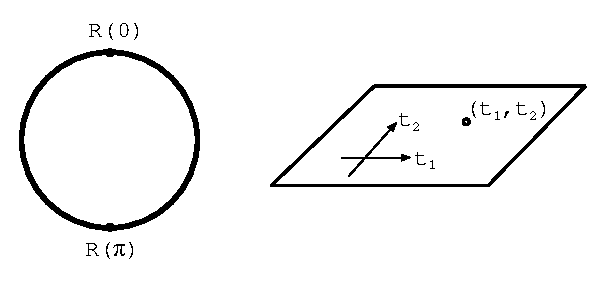
\includegraphics[scale=1.0]{pics/mnogostrukost.eps}}

Kao drugi primjer promotrimo grupu svih translacija u ravnini $\vec{x}\to\vec{x}+\vec{t}$,
dakle translacija za bilo koji vektor $\vec{t}=(t_1, t_2)$.
Ovdje je elemente grupe prirodno parametrizirati dvama
realnim brojevima $t_1, t_2 \in (-\infty, \infty)$ i očito je da je
 grupna mnogostrukost ravnina tj. $\mathbb{R}^2$. Ovdje naravno treba
 razlikovati ravninu koja je vektorski prostor čije vektore transformiraju
 elementi grupe
 (tj. strogo uzevši njene reprezentacije) i ravninu koja je grupni prostor za koji uopće
 nije nužno da ima svojstva vektorskog prostora.

Kako vidimo iz ova dva primjera, elemente kontinuiranih grupa identificiramo
s točkama $n$-dimenzionalne grupne mnogostrukosti koju
parametriziramo s $n$ realnih brojeva
  $(a_1, a_2, \ldots, a_n)$,
te onda govorimo o \emph{$n$-parametarskoj} ili \emph{$n$-dimenzionalnoj} grupi.
Zahvaljajući toj identifikaciji
elemente grupe ćemo označavati kao $g(a_1, a_2, \ldots, a_n)$, odnosno
skraćeno $g(a)$.

Promotrimo sada četiri aksioma grupe u svjetlu ove diskusije.
\begin{enumerate}
\item Zatvorenost: $g(c)=g(a)g(b) \in G$. Umjesto tablice množenja koja
    je definirala grupnu operaciju, sada nam treba funkcija, tzv.
    funkcija kompozicije
    \[\phi: G\times G \to G \quad  \text{tako da je} \quad c=\phi(a,b) \]
    (Npr. za rotacije oko date osi imamo $R(\theta) = R(\theta_1) R(\theta_2)$
    gdje je funkcija kompozicije  $\theta = \phi(\theta_1, \theta_2) =
    (\theta_1 + \theta_2)\, \mathrm{mod}\, 2\pi$ .) U svjetlu identifikacije
    grupe i njenog grupnog prostora ovdje pišemo da je grupa $G$ domena i kodomena funkcije $\phi$
    premda je to strogo uzevši grupni prostor.

\item Asocijativnost: $g(a)\big[g(b)g(c)\big]=\big[g(a)g(b)\big]g(c)$ što
    znači da funkcija kompozicije mora zadovoljavati
    $\phi(a, \phi(b,c))=\phi(\phi(a,b),c) $.

\item Identiteta: postoji parametar $a^0$ takav da je 
       $g(a^0)g(a)=g(a)g(a^0)=g(a)$ za sve parametre $a$.
    Običaj je grupnu mnogostrukost parametrizirati tako da bude $a^0=(0, 0, \ldots, 0)
     \equiv 0$ tj. $g(0)=e$ što onda znači da za funkciju
     kompozicije vrijedi $\phi(0,a)=\phi(a,0)=a$.

\item Inverz: $\forall a\quad \exists \bar{a} \td g(a)g(\bar{a})=
        g(\bar{a})g(a)=g(0)=e$ tj. $g(\bar{a})=g(a)^{-1}$. To znači
        da postoji tzv. funkcija inverza
        \[ \psi:G\to G   \quad  \text{tako da je} \quad \bar{a}=\psi(a) \,. \]

\end{enumerate}

Sami aksiomi grupe ne traže nikakvu povezanost između grupnih i topoloških
svojstava grupe. To znači da bi točke grupne mnogostrukosti mogle u načelu biti
pridružene elementima grupe na proizvoljan diskontinuirani pa čak i "ispremješani"
način. Međutim za grupe od interesa preslikavanja između grupne mnogostrukosti
i grupe su "glatka" i takve grupe onda zovemo Lieve.

\begin{definicija}[Lieva grupa]
  Lieva grupa je grupa za koju su funkcije kompozicije
($\phi$) i inverza ($\psi$) diferencijabilne\footnote{Strogo uzevši, 
    dovoljna je kontinuiranost funkcija jer ona u ovom slučaju povlači diferencijabilnost.
 Ta vrlo netrivijalna činjenica da algebarski aksiomi
 grupe osiguravaju da kontinuirane funkcije nužno budu i diferencijabilne
 je sadržaj rješenja 5. Hilbertovog problema.}.
\end{definicija}

Zahtjev da su te funkcije diferencijabilne daje Lievim grupama mnoštvo važnih svojstava,
kako ćemo vidjeti u sljedećem odjeljku.
Ova svojstva se ogledaju
u činjenici da je element $g(a)$ "blizu" elementa $g(a+\delta a)$ te da
da je $\phi(a+\delta a, b)$
"blizu" $\phi(a,b)$ tj. te su vrijednosti povezane Taylorovim redom.
\centerline{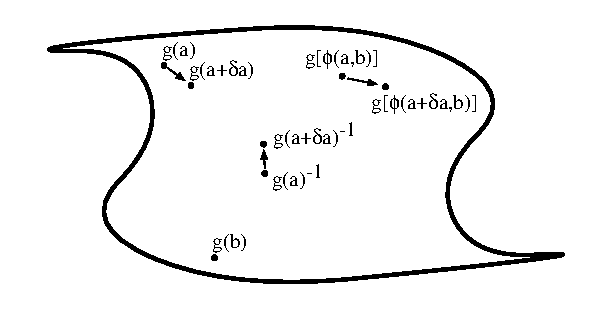
\includegraphics[scale=1.0]{pics/lieva_mnogostrukost.eps}}
Tako teorija Lievih grupa spaja ideje iz algebre, analize i geometrije.

Analiza općenitih Lievih grupa, koja se oslanja samo na ovu definiciju
je matematički dosta zahtjevna. Srećom praktički sve Lieve grupe koje se javljaju
u fizici mogu se vjerno reprezentirati matricama i mi ćemo se baviti
samo takvim tzv. matričnim Lievim grupama. Smanjenje općenitosti je neznatno\footnote{Za
    znatiželjne, primjeri ne-matričnih Lievih grupa su uvijek egzotični
    poput tzv. metaplektičkih grupa ili kvocijentne grupe Heisenbergove grupe po
jednoj svojoj specifičnoj normalnoj podgrupi.\label{fus:nematricne}},
a rad s matricama je značajno lakši od rada s diferencijabilnim mnogostrukostima.
Na primjer, matrice odmah dolaze parametrizirane brojčanim vrijednostima svojih
elemenata. Tu je važno
ne pomiješati dimezionalnost matrične grupe s dimenzionalnošću njenih matrica.
Kako je rečeno gore, dimenzionalnost grupe je jednaka broju \emph{nezavisnih realnih}
parametara koji specificiraju element grupe tj. matricu. Tako je grupa rotacija
u ravnini dana dvodimenzionalnim matricama
\begin{equation}
    \left\{ \begin{pmatrix}
        \cos\phi & -\sin\phi \\
        \sin\phi & \cos\phi 
    \end{pmatrix} 
     \td \phi \in [0, 2\pi) \right\} \,,
    \label{eq:so2}
\end{equation}
ali to je jednodimenzionalna grupa jer je svaka matrica potpuno određena
jednim realnim parametrom $\phi$. Matrične grupe imaju svoja klasična
imena pa se tako grupa iz (\ref{eq:so2}) zove \SO{2}, što dolazi
od \emph{specijalna} ($\det M = 1$) \emph{ortogonalna} ($M^\mathsf{T} M = 1$) 
grupa $2\times 2$ matrica.



\section{Lieve algebre}
\label{sec:lievealgebre}

Promotrimo sada skup matrica $M(a)\equiv M(a_1, a_2, \ldots, a_n)$ koje
čine $n$-pa\-ra\-me\-tar\-sku Lievu grupe.
Za infinitezimalno male vrijednosti parametara $a_i \to \epsilon_i \ll 1$, zahvaljujući
svojstvu diferencijabilnosti Lieve grupe možemo razviti oko $a_i = 0$:
\begin{equation}
   M(\epsilon)=M(0)+ \sum_{i=i}^{n}\epsilon_i \frac{\partial M(a_1, \ldots, a_n)}
 {\partial a_i}\Bigg|_{a_1=\ldots =a_n=0} + 0(\epsilon^2) \,,
 \label{eq:razvojM}
\end{equation}
gdje diferenciranje matrica provodimo prirodno diferencirajući svaki njen
element ponaosob. Koeficijenti od $\epsilon_i$ u (\ref{eq:razvojM}) su
konstantne matrice (ne ovise o parametrima) koje se nazivaju generatori
i skraćeno ćemo ih označiti s $X_i$
\begin{equation}
X_i =  \frac{\partial M(a_1, \ldots, a_n)}
 {\partial a_i}\Bigg|_{a_1=\ldots =a_n=0} = \textrm{const}(a_1, \ldots, a_n)
   \quad i=1, \ldots, n 
   \label{eq:defXi}
\end{equation}
Očito je da generatora ima koliko i parametara tj. njihov broj je jednak
dimenzionalnosti grupe (grupne mnogostrukosti).  $M(0)$ je jedinični
element grupe tj. jedinična matrica pa za infinitezimalne transformacije imamo
\begin{equation}
  M(\epsilon)=\Eins + \sum_{i=i}^{n}\epsilon_i X_i \,. 
\end{equation}

Centralna spoznaja teorije Lievih grupa je da je struktura \emph{čitave} grupe i
njenih reprezentacija skoro sasvim određena
određena generatorima grupe tj. infinitezimalnom okolinom jediničnog 
elementa.
Ovo ćemo većim dijelom samo pokazati na primjeru grupe rotacija realnog
trodimenzionalnog euklidskog prostora, a za općeniti
dokaz čitaoc može konzultirati literaturu poput \cite{Stilwell:2008}.

Transformacije prostora koje čuvaju udaljenosti između točaka, a time
i iznose (duljine) vektora, nazivaju se \emph{izometrije}. U vektorskim prostorima,
udaljenost se prirodno definira pomoću skalarnog produkta vektora $(\vec{x}, \vec{y})$
tako da je iznos vektora $\sqrt{(\vec{x}, \vec{x})}$,
a izometrije će onda biti transformacije koje čuvaju skalarni produkt. Zapišemo
li to pomoću matrica vidimo da matrica izometrije $R$ mora zadovoljavati
\begin{equation}
    (Rx, Ry) = \sum_{ijk} R_{ij}x_{j} \, R_{ik} y_{k} = \sum_{ijk} x_{j} (R^\mathsf{T})_{ji}
    \, R_{ik} y_{k} = (x, R^{\mathsf{T}} R y) \stackrel{!}{=} (x, y) \,,
\end{equation}
pa mora biti $R^{\mathsf{T}} R = 1$, a matrice koje to zadovoljavaju
nazivamo \emph{ortogonalne} jer iz tog svojstva slijedi da su retci i stupci
tih matrica ortogonalni vektori, štoviše ortonormirani su. Grupa svih
ortogonalnih $3 \times 3$ matrica se naziva \O{3}.

Kako je prema Binet-Cauchyjevom teoremu $\det R^\mathsf{T} R = \det R^\mathsf{T} \det R$,
te kako transpozicija ne mijenja determinantu, vidimo da je $(\det R)^2 = 1$,
pa determinanta ortogonalne matrice može biti samo 1 ili -1.
Matrice s determinantom -1, poput 
\begin{equation}
\begin{pmatrix}
\cos\phi & -\sin\phi & 0 \\
\sin\phi & \cos\phi & 0 \\
0 & 0 & -1 \end{pmatrix} \,,
\end{equation}
daju transformaciju koja je kombinacija rotacije i refleksije preko
neke ravnine kroz ishodište (u ovom primjeru to je $x$-$y$ ravnina).
Refleksije također čuvaju
udaljenosti, ali ne čuvaju orijentaciju (lijevi vijak se
se pretvara u desni). Tako je grupa svih rotacija dana skupom ortogonalnih
matrica determinante 1 i naziva se \emph{specijalna} ortogonalna grupa \SO{3}.
U odjeljku \ref{sec:primjeriLie} dokazat ćemo da je ta grupa troparametarska,
no to je i odmah jasno ako znamo da su rotacije potpuno specificirane pomoću
tri Eulerova kuta.

Promotrimo sada jednoparametarsku podgrupu grupe \SO{3} koju čine
rotacije oko treće tj. $z$-osi.
\begin{displaymath}
\left\{ R_3 (\phi) = 
\begin{pmatrix}
\cos\phi & -\sin\phi & 0 \\
\sin\phi & \cos\phi & 0 \\
0 & 0 & 1 
\end{pmatrix}
 \td \phi \in [0, 2\pi) \right\} = \SO{2} = \subset \SO{3} \,,
\end{displaymath}
gdje premda su same matrice $R_3 (\phi)$ trodimenzionalne one su
naravno izomorfne grupi \SO{2} rotacija $x$-$y$ ravnine.
Generator te pogrupe je
\begin{equation} \label{eq:x3so3}
X_3 = \frac{\partial R_3 (\phi)}{\partial \phi}\Bigg|_{\phi=0}=
\begin{pmatrix}
-\sin\phi & -\cos\phi & 0 \\
\cos\phi & -\sin\phi & 0 \\
0 & 0 & 1 
\end{pmatrix}\Bigg|_{\phi=0} =
\begin{pmatrix}
0 & -1 & 0 \\
1 & 0 & 0 \\
0 & 0 & 0 
\end{pmatrix} \,,
\end{equation}
i infintezimalna rotacija oko $z$-osi je $R_3 (\epsilon) = 1 + \epsilon X_3$.
Ideja je sada komponirati $N$ ovih rotacija za infinitezimalni kut
$\epsilon$ i uočiti da
će u limesu $N \to\infty$ uz $N\epsilon \to \phi$ 
takva kompozicija rezultirati rotacijom za proizvoljni \emph{konačni}
kut $\phi$
\begin{displaymath}
[R_3(\epsilon)]^{N} = (1+\epsilon X_3)^N = \left(1+\frac{(N\epsilon)X_3}
 {N}\right)^N 
 \xrightarrow[\substack{N \to \infty \\ (N\epsilon) \to \phi}]{}
 e^{\phi X_3} \,,
\end{displaymath}
gdje smo upotrijebili svojstvo eksponencijalne funkcije
\begin{equation}
    \lim_{N\to\infty}\left(1 + \frac{x}{N}\right)^N = \exp(x) \,,
\end{equation}
koje vrijedi za broj $x$,
u nadi da će ono vrijediti i kad je $x$ matrica.
U dodatku \ref{sec:expmat} diskutiramo
kako eksponenciranje matrica zaista funkcionira isto kao i
eksponenciranje brojeva, uz još neka dodatna zanimljiva svojstva,
te tamo usput eksplicitno pokazujemo da je
\begin{equation}
e^{\phi X_3} = \exp\Bigg\{ 
    \phi  \begin{pmatrix}
0 & -1 & 0 \\
1 & 0 & 0 \\
0 & 0 & 0 
\end{pmatrix}\Bigg\} =
\begin{pmatrix}
\cos\phi & -\sin\phi & 0 \\
\sin\phi & \cos\phi & 0 \\
0 & 0 & 1 \end{pmatrix} \,.
\end{equation}
Tako vidimo da zaista svaki element ove jednoparametarske podgrupe
od \SO{3} možemo dobiti eksponencijacijom generatora.
Nadalje, u skladu s Eulerovim teoremom iz mehanike\footnote{Svaki pomak krutog
tijela kod kojeg jedna točka ostaje nepomična je ekvivalentan \emph{jednoj}
rotaciji oko fiksne osi koja prolazi kroz tu točku.} svaka \SO{3} rotacija 
pripada nekoj jednoparametarskoj podgrupi
 (čine je sve rotacije oko te iste osi), što onda znači da se
svi elementi grupe \SO{3} mogu se dobiti eksponencijacijom generatora.
Mogućih osi rotacije ima beskonačno pa tako i geratora ima beskonačno
i pitanje je kako ih odrediti.
Kako se vidi iz (\ref{eq:defXi}) konkretan oblik generatora ovisi
o parametrizaciji grupnog prostora. 
Mogli bismo recimo pokušati konstruirati opću rotaciju kao kompoziciju tri
 Eulerove rotacije i onda deriviranjem po Eulerovim kutovima dobiti
 generatore. No, ima i lakši put koji će olakšati traženje 
 generatora drugih Lievih grupa koje se pojavljuju u fizici\footnote{Recimo
     usput i da bi pristup preko Eulerovih
     bio  problematičan jer su one singularne oko jedinice.}.

Oslonit ćemo se na definiciju \SO{3} kao grupe svih 
3$\times$3 matrica $R$ sa svojstvom  $RR^{T}=1$ i $\det R=1$.
Rotacije za infinitezimalni kut imat će oblik  $R(\epsilon)=1+\epsilon X$,
gdje je $X$ jedan od generatora. Uvjet ortogonalnosti je sada
\begin{equation}
 RR^{T}=(1+\epsilon X)(1+\epsilon 
   X^{T}) = 1+\epsilon (X+X^{T})+0(\epsilon^2) = 1 \,,
\end{equation}
što znači da je $X^\mathsf{T}=-X$ odnosno $X$ je antisimetrična 3$\times$3 matrica.
Obratno, ako je $X$ antisimetrična, njena eksponencijacija $R = e^X$ daje ortogonalnu
matricu jer je
\begin{equation}
  R R^\mathsf{T} = e^X (e^X)^\mathsf{T} = e^X e^{X^\mathsf{T}}
  = e^X e^{-X}
  = e^{X-X} = 1 \,,
\end{equation}
gdje je jedini netrivijalni korak predzadnji. Naime, vidi dodatak \ref{sec:expmat},
$e^{A} e^{B} = e^{A+B}$ samo ukoliko matrice $A$ i $B$ komutiraju što je ovdje
srećom trivijalno slučaj.
Zahvaljujući općenitoj relaciji $\det e^{X} = e^{\textrm{\scriptsize Tr} X}$,
vidi dodatak \ref{sec:expmat}, te činjenici da antisimetrične matrice imaju
nule na glavnoj dijagonali, uvjet specijalnosti determinante $\det R = 1$ je
zadovoljen automatski.
Tako smo pokazali da skup $\calA$ svih antisimetričnih 3$\times$3 matrica
generira grupu \SO{3}\footnote{Pažljivi čitaoc će možda u ovom automatskom
    zadovoljenju uvjeta $\det R =1$ vidjeti kontradikciju:
 Refleksije su isto ortogonalne matrice,
pa bi i njihovi generatori trebali biti antisimetrični, no njihova determinanta
je -1. Stvar je u tome da refleksije nije moguće generirati kompozicijom
infinitezimalnih transformacija tj. one nemaju generatore. O tome će još biti
govora kasnije.\label{fus:refleksija}
}.

Skup generatora $\calA$ ima i dodatna svojstva. Kao prvo, on je
vektorski prostor nad poljem $\mathbb{R}$ jer za svaka dva vektora
$X_1, X_2\in\calA$ i svaka dva broja $\alpha, \beta\in\mathbb{R}$ 
$(\alpha X_1 + \beta X_2)$ je isto antisimetrična matrica, a time i
element $\calA$. Dimenzija od $\calA$ je 3 jer je najopćenititiji
oblik $3\times 3$ antisimetrične matrice
\begin{equation}
    \begin{pmatrix}
        0 &  a  &  b \\
       -a &  0  &  c \\
       -b & -c  &  0
   \end{pmatrix}  \qquad   a, b, c \in \mathbb{R} \,.
\end{equation}
Jednakost dimenzija vektorskog prostora generatora $\calA$ i grupe \SO{3} koju
oni generiraju naravno nije slučajna obzirom da eksponencijacijom
generatora trebamo moći dobiti skoro sve elemente grupe, a u najmanju ruku
barem sve elemente u nekoj okolini jedinice.

Trodimenzionalni vektorski prostor ima tročlanu bazu i u ovom slučaju je
uobičajeno kao bazu izabrati generatore jednoparametarskih podgrupa rotacija oko
$x$, $y$ i $z$ osi. Ovaj treći smo već odredili u (\ref{eq:x3so3}), a kompletna
baza je
\begin{equation}
X_1=
\begin{pmatrix}
0 & 0 & 0 \\ 
0 & 0 &-1 \\
0 & 1 & 0
\end{pmatrix}  \quad
X_2=
\begin{pmatrix}
0 & 0 & 1 \\ 
0 & 0 & 0 \\
-1& 0 & 0
\end{pmatrix}  \quad
X_3=
\begin{pmatrix}
0 & -1 & 0 \\ 
1& 0 & 0 \\
0 & 0 & 0
\end{pmatrix} \,,
\label{eq:SO3generators}
\end{equation}
pa je $e^{\phi \vec{X}\cdot\unitn}$ onda općeniti element grupe \SO{3} koji
predstavlja rotaciju oko osi $\unitn$ za kut $\phi$.

Vektorski prostor sa svojom dodatnom operacijom množenja
skalarima iz polja $\mathbb{R}$ je općenito znatno bogatija struktura od grupe (koja
ima samo svoju binarnu operaciju). To znači da o generatorima "znamo više" i
lakše je proučavati njih i onda pomoću eksponencijacije vidjeti reperkusije tih
spoznaja na samu grupu.
To je dodatno pojačano još jednim njihovim važnim svojstvom.
Neka su $X,Y\in\calA$. Definirajmo njihov \emph{komutator} 
\begin{equation}
    [X, Y] \equiv X Y - Y X \,.
    \label{eq:defkomutator}
\end{equation}
Komutator je također $3\times 3$ matrica koja je štoviše također antisimetrična
jer
\begin{equation}
 [X,Y]^\mathsf{T} = (XY-YX)^\mathsf{T} = Y^\mathsf{T} X^\mathsf{T} - X^\mathsf{T} Y^\mathsf{T}
 = YX-XY = -[X,Y] \,.
\end{equation}
To znači da je i komutator $[X,Y]\in\calA$.
Dakle, $\calA$ je zatvoren ne samo obzirom na linearne kombinacije već
i obzirom na komutatore svojih elemenata. Time je on još složenija matematička
struktura od vektorskog prostora koja se naziva  \emph{Lieva algebra}.
Načinimo kratki odmak od proučavanja samo matričnih grupa i
definirajmo Lievu algebru nešto općenitije.
\begin{definicija}[Lieva algebra]
Lieva algebra $\calA$ je vektorski prostor na kojem je definiran 
Liev produkt dvaju elemenata $[X,Y]$ (ne mora biti komutator) sa svojstvima

1) zatvorenost: $[X,Y]\in\calA \quad \forall X,Y\in\calA$

2) distributivnost: $[\alpha X + \beta Y, Z]=\alpha[X,Z]+\beta[Y,Z]$
$\quad \alpha,\beta \in \mathbb{R} $

3) antisimetrija: $[X,Y]=-[Y,X]$

4) Jacobijev identitet: $[X, [Y, Z]]+[Y, [Z, X]]+[Z, [X, Y]]=0$
\end{definicija}
Za vektorske prostore matrica, gdje je Liev produkt definiran kao
komutator (\ref{eq:defkomutator}), svojstva 2--4 su automatski ispunjena.
Ovo poopćenje od matričnih grupa smo napravili samo zato da kao
spomenemo da zapravo o nikakvom poopćenju nema govora.
Naime, kako smo rekli u fusnoti na stranici \pageref{fus:nematricne}, nematrične Lieve grupe
su egzotične, ali postoje. No, zahvaljujući sljedećem Adovom teoremu
nematrične (konačno-dimenzionalne) Lieve algebre ne postoje.
\begin{teorem}[Ado]
 Svaka konačno-dimenzionalna apstraktna Lieva algebra je izomorfna nekoj
 Lievoj algebri konačno-dimenzionalnih matrica s komutatorom kao Lievim produktom. \emph{(Bez
 dokaza.)}
\end{teorem}
Dakle, ograničavajući se na Lieve grupe \emph{matrica} ne gubimo mnogo
na općenitosti jer sve Lieve algebre koje ćemo sresti u ovoj knjizi su
konačno-dimenzionalne\footnote{Istina, u fizici nekad nalazimo i primjenu beskonačno-dimenzionalnih
algebri za koje teorem ne vrijedi. Jedan primjer je tzv. Virasorova algebra važna
u teoriji superstruna.}.
Lieve algebre se obično označavaju isto kao i pripadajuće Lieve grupe, ali malim gotičkim slovima.
Dakle, $\calA = \soAlg{3}$.

Komutatori elemenata baze Lieve algebre $X_i, i=1,2,\ldots, \textrm{dim}(\calA)$ se
kao i svi ostali elementi od $\calA$ naravno mogu prikazati kao linearna kombinacija baze, dakle
sebe samih: 
\begin{equation}
 [X_i, X_j]= \sum_k C_{ij}^{k} X_k \,,  \qquad i,j=1,2,\ldots, \textrm{dim}(\calA) \,.
 \label{eq:defstrukturne}
\end{equation}
Realni brojevi $C_{ij}^{k}$ koji se ovdje pojavljuju nazivaju se \emph{strukturne konstante} grupe.
Uočite da je (\ref{eq:defstrukturne}) vrlo netrivijalna nelinearna relacija između
generatora koju će morati zadovoljavati sve njihove reprezentacije.  Naime, cijelo ovo
izlaganje dosad koristilo je $3\times 3$ matrice za definiciju grupe \SO{3} i njene
algebre \soAlg{3}. To je istovremeno i definicija te grupe i reprezentacija te grupe 
na 3D euklidskom prostoru.
Međutim, slično kao i kod konačnih grupa, Lieve grupe imaju i
reprezentacije na vektorskim prostorima drugih dimenzionalnosti, što je od velike
važnosti u primjeni teorije grupa na kvantnomehaničke sustave. I tu će opet biti od interesa
identificirati sve ireducibilne reprezentacije neke grupe. Koliko ireducibilnih
reprezentacija očekujemo? Ako bismo se oslonili na fundamentalni rezultat iz teorije
konačnih grupa da ireducibilnih reprezentacija ima isto koliko i klasa konjugacije,
vidi odjeljak \ref{sec:ortogonalnost}, onda bismo zaključili da \SO{3} ima beskonačno
ireducibilnih reprezentacija (jer se uz malo geometrijskog razmišljanja lako uvjerite
da pojedinu klasu konjugacije čine rotacije oko bilo koje osi za konkretni kut $\phi$).
I premda je takvo zaključivanje nekorektno jer navedena jednakost broja ireducibilnih
reprezentacija i klasa konjugacije \emph{ne vrijedi} za Lieve grupe, zaključak jest
točan --- Lieve grupe tipično imaju beskonačno ireducibilnih reprezentacija.
Jedna od lako uočljivih razlika prema konačnim grupama je u tome da premda
\SO{3} ima neprebrojivo beskonačno klasa konjugacije, vidjet ćemo da ima samo prebrojivo
beskonačno ireducibilnih reprezentacija.
Bez obzira, očito je da nećemo moći eksplicitno konstruirati sve te repreprezentacije
metodom nadopunjavanja tablice karaktera iz odjeljka \ref{sec:karakteri},
nego apstraktnijim zaključivanjem u kojem će
relacija (\ref{eq:defstrukturne}), koju fizičari često zovu "algebra grupe," imati
centralnu ulogu, kako ćemo vidjeti u sljedećim poglavljima.
Kad smo već kod terminologije, recimo i to da je fizičarima često interes usredotočen
samo na bazu Lieve algebre, a ne i na ostatak vektorskog prostora, pa će u žargonu
reći da tri matrice iz (\ref{eq:SO3generators}) "čine algebru" ove grupe.


\begin{primjer}[strukturne konstante od \SO{3}]
Eksplicitnim računom lako se uvjerimo da je
 \begin{align}
     [X_i,X_j]& =0 \quad\text{za}\quad i=j \,,  \\
     [X_1,X_2]& = X_3 \,, \\
     [X_2,X_3]& = X_1  \,, \\
     [X_3,X_1]& = X_2 \,,
 \end{align}
tj. da je
\begin{align}
 C_{ij}^{k}& = 0 \quad\text{ako su bilo koja dva indeksa ista} \,, \\
 C_{12}^3  & = C_{23}^{1}=C_{31}^{2}=1 \,, \\
 C_{21}^3  & = C_{32}^{1}=C_{13}^{2}=-1 \,, \\
 \end{align}
pa pomoću Levi-Civita tenzora
komutacijske relacije algebre \soAlg{3} možemo zapisati u obliku
\begin{equation}
 [X_i, X_j]=\epsilon_{ijk} X_k  \,,
  \label{eq:algebraso3}
\end{equation}
odnosno strukturne konstante grupe \SO{3} su $C_{ij}^{k} = \epsilon_{ijk}$.
\end{primjer}


Lieva algebra $\calA'$ je \emph{homomorfna} Lievoj algebri $\calA$ ako postoji 
matrica $S:\calA\to\calA'$ takva da je
\begin{displaymath}
       [S(X), S(Y)]=S([X,Y]) \quad \forall X, Y \in\calA \,.
\end{displaymath}
Ako je $S$ još i bijekcija $\calA$ i $\calA'$ su \emph{izomorfne}. Dakle,
važno je da preslikavanje  bude konzistentno s operacijom komutatora.

\begin{primjer}[Lieva algebra grupe \SU{2} tj. \suAlg{2}]
    \SU{2} je grupa svih unitarnih $2\times 2$ matrica jedinične determinante.
    Identičnim zaključivanjem kao za \SO{3}, samo uz zamjenu traspozicije
    hermitskom konjugacijom $X^\mathsf{T} \to X^\mathsf{\dagger}$ lako
    zaključujemo da algebru \suAlg{2} čine sve
    antihermitske\footnote{$A$ je antihermitska ako je $A^\dagger=-A$} 
    2$\times$2 matrice s tragom nula (ovdje zadovoljavanje uvjeta jedinične
    determinante nije automatsko). Kao bazu ove algebre uzimamo
\begin{equation}
     \{ -i\frac{\sigma_1}{2},  -i\frac{\sigma_2}{2},  -i\frac{\sigma_3}{2} \} \,,
\end{equation}
gdje su $\sigma_{1,2,3}$ tri Paulijeve matrice
\begin{equation}
\sigma_1=\left( \begin{array}{cc} 0 &  1 \\ 1 & 0 \end{array} \right) \,,
\quad
\sigma_2=\left( \begin{array}{cc} 0 & -i \\ i & 0 \end{array} \right) \,,
\quad
\sigma_3=\left( \begin{array}{cc} 1 &  0 \\ 0 &-1 \end{array} \right) \,.
\label{eq:PaulijeveMatrice}
\end{equation}
Ova tri generatora zadovoljavaju identične komutacijske relacije kao i matrice
\soAlg{3} algebre
\begin{displaymath}
 \left[ -i\frac{\sigma_1}{2}, -i\frac{\sigma_2}{2} \right] =
 -i\frac{\sigma_3}{2} \qquad \text{itd.}
\end{displaymath}
pa je pridruživanje $X_i \to -i \sigma_i/2$  izomorfizam i
\soAlg{3}=\suAlg{2}.

Važno je ovdje uočiti da premda su elementi matrica iz \suAlg{2} općenito kompleksni,
\suAlg{2} je \emph{realna} Lieva algebra, dakle algebra nad poljem $\mathbb{R}$. 
(Linearna kombinacija $\sigma_1 + \sigma_2$ je antihermitska i time pripada \suAlg{2},
dok $\sigma_1 + i \sigma_2$ to nije!)

Zanimljivo je pitanje što izomorfizam algebri znači za odgovarajuće grupe tj.
jesu li možda onda i \SO{3} i \SU{2} izomorfne. O tome će biti riječi u sljedećem poglavlju.
\end{primjer}

Pri analizi reprezentacija Lievih grupa od koristi će biti
tzv. Casimirovi operatori.
\begin{definicija}[Casimirov operator]
Ako je skup $\{X_i, i=1,2, ... \}$ baza Lieve algebre onda se polinom
u $X_i$ koji komutira sa svim elementima te algebre naziva 
\emph{Casimirov operator}.
\end{definicija}
Posebno su zanimljivi kvadratični Casimirovi operatori.
\begin{primjer}[Kvadratični Casimirov operator za \soAlg{3} i \suAlg{2}]
 Eksplicitnim računom se uvjerimo da je 
\begin{equation}
X_{1}^2 + X_{2}^2 + X_{3}^2 = -2\cdot \Eins \,,
\end{equation}
    za \soAlg{3} i
\begin{equation}
    \left(\frac{-i}{2}\right)^2
    \big(\sigma_{1}^2 + \sigma_{2}^2 + \sigma_{3}^2\big) = -\frac{3}{4} \cdot \Eins \,,
\end{equation}
    za \suAlg{2}.
\end{primjer}
Schurova lema, koja vrijedi i za Lieve grupe, traži da Casimirov operator 
bude proporcionalan jediničnom i ispostavlja se da je koeficijent proporcionalnosti
zgodan za označavanje ireducibilnih reprezentacija kako ćemo vidjeti u sljedećem poglavlju.



\section{Veza Lievih grupa i Lievih algebri}

Vidjeli smo da u slučaju grupe \SO{3} 
\emph{svaki} element grupe možemo prikazati kao eksponencijal nekog
elementa njene Lieve algebre \soAlg{3}.
Pitanje je vrijedi li to lijepo svojstvo za sve Lieve grupe.
Kako smo već dali naslutiti na nekoliko mjesta upotrijebom riječi "skoro",
ne vrijedi sasvim. U ovom ćemo odjeljku, uglavnom
bez dokaza, iskazati i pomoću primjera ilustrirati tvrdnje koje 
pobliže oslikavaju vezu između Lievih grupa i njihovih algebri.
Za većinu primjena u fizici i u ostatku knjige, uglavnom ćemo
se fokusirati na algebre i reprezentacije algebri, tako da (razmjerno
zahtjevno) gradivo ovog odjeljka nije nužno za razumijevanje sljedećih
poglavlja.

Prvo je potrebno uvesti neke pojmove koji opisuju topološka
svojstva grupe.
\begin{definicija}[Povezanost]
Lieva grupa je \emph{povezana} ako njen grupni prostor ne možemo
rastaviti na disjunktne komponente tj. ako se svake dvije točke 
mogu povezati linijom čije sve točke pripadaju grupnom prostoru.
(Ovo je intuitivna "fizičarska" definicija. Prava definicija uključuje napredne
matematičke ideje iz topologije.)
\label{def:povezanost}
\end{definicija}
Podskup kojeg čine svi elementi grupe koji se
kontinuiranom linijom u grupnoj mnogostrukosti mogu povezati s
jediničnim elementom nazivamo \emph{komponenta povezanosti jedinice}.
Ukoliko je grupa povezana komponenta povezanosti jedinice je naravno
jednaka cijeloj grupi. Ukoliko grupa nije povezana, komponenta povezanosti
jedinice je prava podgrupa cijele grupe. \emph{Dokaz}: Pretpostavimo
suprotno tj. da komponenta povezanosti jedinice nije podgrupa. Kako je
jedinični element po definiciji u toj komponenti te kako je asocijativnost
nasljeđena od cijele grupe to bi značilo ili da postoje njena dva elementa čiji
umnožak nije u komponenti povezanosti jedinice ili neki element čiji inverz nije u 
toj komponenti.
Promotrimo sada dva elementa $a$ i $b$ koji jesu, a čiji umnožak $ab$ nije u komponenti
povezanosti jedinice, te promotrimo trajektoriju $g(t)$, $t\in[0,1]$,
definiranu tako da je $g(0)=a$, a $g(1)=e$. Trajektorija dakle
kontinuirano povezuje $a$ s jediničnim elementom $e$.
Pomičući se kontinuirano po toj trajektoriji prema jedinici
umnožak $g(t)b$ će cijelo vrijeme ostati izvan komponente povezanosti jedinice
zbog odvojenosti njegovog dijela grupnog prostora i kontinuiranosti
funkcije kompozicije (umnožak $g(t)b$ ne može "preskočiti" sa svoje odvojene
komponente na komponentu jedinice). No kad dođemo do jediničnog elementa
umnožak je $g(1)b = eb = b$ što po pretpostavci jest element komponente jedinice
i imamo kontradikciju. Na sličan način se do kontradikcije dođe u slučaju inverza.\qed

Eksponencijacijom generatora grupe \SO{3} dolazimo do konačnih rotacija
$\exp(\phi \vec{X}\cdot\unitn)$ trajektorijom koja ide od jediničnog
elementa $\phi=0$ kontinuiranom putanjom kroz grupni prostor, kompozicijom rotacija za
infinitezimalne kuteve. Kako je eksponencijalna funkcija kontinuirana
funkcija svojih argumenata (čak i kad su argumenti matrice), te kako
je determinanta također kontinuirana funkcija, u slučaju grupe \O{3},
za čije elemente smo vidjeli da imaju determinantu ili +1 ili -1,
jasno je da eksponencijacijom algebre možemo dobiti (a u slučaju \O{3}
i dobivamo) samo elemente s determinantom +1, dakle prave rotacije.
Matrice koje imaju determinantu -1 nekad se 
nazivaju \emph{neprave} rotacije i pripadaju drugoj komponenti povezanosti.

Neprave rotacije se mogu na jedinstven
način prikazati kao umnožak običnih rotacija iz \SO{3} i operatora inverzije
\begin{equation}
I = \begin{pmatrix}
-1 & 0 & 0 \\ 
0  &-1 & 0 \\
0  & 0 & -1
\end{pmatrix} \,.
\end{equation}
Naime, uzmemo li proizvoljnu nepravu rotaciju $\tilde{R}$ tada
je zahvaljujući Binet-Cauchyjevom teoremu determinanta matrice
$I \tilde{R}$ svakako +1 pa je ta matrica prava rotacija $I\tilde{R} = R$
i onda je $\tilde{R} = I R$. Tako je cijeli taj skup (nije podgrupa!)
kojeg čine neprave rotacije zapravo jednak umnošku $I\SO{3}$ i vidimo da
se cijela ortogonalna grupa sastoji od točno dvije disjunktne komponente
\begin{equation}
    \O{3} = \SO{3} + I\SO{3}\,,
\end{equation}
koje su, promatrane kao dijelovi grupnog prostora, topološki identične.
Zanimljivo pitanje točnog izgleda ovog grupnog prostora raspravit ćemo malo
kasnije u ovom poglavlju.


Iz gornje diskusije, odnosno imajući u vidu kontinuiranost funkcije
eksponencijacije, jasno da najbolje čemu se možemo nadati u
slučaju općenite Lieve grupe je da
eksponencijacijom njene algebre dobijemo komponentu povezanosti
jedinice. No je li barem to uvijek moguće?
Kako smo pokazali, svakoj Lievoj grupi jednoznačno pripada neka Lieva algebra
konstrukcijom kao u (\ref{eq:defXi}). Možemo li, obratno, svakom
elementu $g$  komponente povezanosti jedinice pridružiti jedinstveni
element $X$ algebre takav da je $g = e^{X}$?

Prije nego damo odgovor na to pitanje, skrenimo pažnju na to da je
povezivanje elemenata algebre i elemenata grupe exponencijacijom
(odnosno u drugom smjeru inverznom funkcijom logaritma) samo dio
posla. Potrebno je pokazati i da je binarna grupna operacija potpuno
određena operacijama s odgovarajućim elementima algebre. Kako
dakle izračunati $e^X e^Y$? Imajuči u vidu definiciju eksponencijacije
to je
\begin{equation}
   e^X e^Y = \left(\sum_{k=0}^{\infty} \frac{X^k}{k!}\right)
             \left(\sum_{n=0}^{\infty} \frac{Y^n}{n!}\right)
    \,,
\end{equation}
i nije odmah jasno da se desna strana može dobiti eksponencijacijom nekog
elementa algebre, osim u jednostavnom slučaju Abelove grupe kad je 
$[X, Y]=0$ (vidi zadatak \ref{zad:abelovaalgebra}) pa se članovi
gornjih suma mogu isto kao kod eksponencijacije običnih brojeva
iskombinirati u $\sum (X+Y)^{n}/n! = \exp(X+Y)$. Za općenite
nekomutirajuće grupe to nije slučaj, nego vrijedi važan
rezultat teorije Lievih grupa
\begin{teorem}[Baker-Campbell-Hausdorff]
    \[ e^X e^Y = e^Z \,, \]
  gdje je 
  \[ Z = X + Y + \text{red višestrukih komutatora $X$ i $Y$.} \]
\end{teorem}
Prvi članovi BCH formule su
\begin{align}
    Z& = X + Y + \frac{1}{2}[X, Y] + \frac{1}{12}[X, [X, Y]] 
       - \frac{1}{12}[Y, [X, Y]] \nonumber \\
     &   - \frac{1}{24}[X, [Y, [X, Y]]] + \frac{1}{720}[Y, [Y, [Y, [X, Y]]]] 
         + \cdots \,,
\end{align}
i ključna netrivijalnost je da su \emph{svi} članovi reda dati preko
ovakvih višestrukih komutatora pa je jasno da je $Z$ element Lieve algebre.
(Podsjetimo se da je u Lievoj algebri definirano zbrajanje elemenata $X+Y$ i njihov
 komutator $[X, Y]$, ali ne i množenje\footnote{Ako gledamo matrične
    Lieve algebre množenje zapravo jest definirano, ali algebra općenito nije zatvorena
    na to množenje. Npr. umnožak dvije antisimetrične matrice iz \soAlg{3} 
    općenito \emph{nije} antisimetrična matrica.} $X Y$.)
BCH red konvergira u nekoj okolini jediničnog elementa (ne nužno infinitezimalnoj)
i u toj okolini je grupa potpuno i jedinstveno određena algebrom.
Eksponencijacija povezuje elemente grupe i algebre, a BCH formula
operacije u algebri (zbrajanje i komutator) s grupnom operacijom (množenje).
Dokaz i razmatranje radijusa konvergencije BCH formule
obično zahtijeva napredne matematičke
pojmove. Relativno pristupačan algebarski dokaz može se pronaći
u \cite{Stilwell:2008}.

Za veliku kategoriju Lievih grupa vrijedi da se svi elementi iz 
komponente povezanosti jedinice mogu prikazati u obliku
$e^{X}$ gdje je $X$ element
Lieve algebre. Dovoljan uvjet je da grupa ima svojstvo \emph{kompaktnosti}.
\begin{definicija}[Kompaktnost]
Lieva grupa je \emph{kompaktna} ako njeni parametri variraju po zatvorenim intervalima.
(Ovo je intuitivna "fizičarska" definicija. Prava definicija uključuje napredne
matematičke ideje iz topologije.)
\label{def:kompaktnost}
\end{definicija}
Mnoge grupe koje će nas interesirati, poput
\SO{n} i \SU{n} su kompaktne, jer njihovi parametri tipično variraju
po intervalima poput $\phi \in [0, 2\pi)$. Iznimka je
grupa translacija, čiji parametri variraju po intervalu $(-\infty,
\infty)$ i grupa Lorentzovih transformacija, čiji parametar
potiska varira $v \in [0, c)$, gdje $c$ nije uključen i stoga
je interval otvoren i nekompaktan\footnote{Radi
    kompletnosti spomenimo da ako Lieva grupa nije kompaktna, 
    svejedno se elementi iz komponente
povezanosti jedinice mogu prikazati kao konačan umnožak eksponencijala
$e^{X_1} e^{X_2}\cdots e^{X_n}$.
Treba razlikovati situaciju gdje se svaki element
grupe (ili njenog podskupa) može dobiti eksponencijacijom (exp
je surjektivna) i situaciju gdje se on može se dobiti na jedinstven način 
(exp je i injektivna).
Injektivnost je zahtjevnije svojstvo. 
Treba uočiti da se algebra grupe \SO{2} preslikava na grupu neinjektivno,
pa nijedna grupa koja
je sadrži kao podgrupu, kao \SO{3}, \SU{2} etc., neće biti injektivno pokrivena
exponencijacijom. Surjektivnost je lakše postići.
Za to je dovoljna kompaktnost,
a može i jednostruka povezanost.}.


Dakle, Lieva algebra skoro potpuno određuje barem komponentu povezanosti
jediničnog elementa Lieve grupe koju generira eksponecijacijom.
Međutim, primjer grupa \SO{3} i \SO{2} koje su obje povezane i koje
imaju istu (izomorfnu) algebru, ali ipak nisu izomorfne, pokazuje
da neka svojstva grupe nisu određena algebrom, tj. da "skoro" iz
prošle rečenice ipak nije "potpuno."
Riječ je o globalnim topološkim svojstvima grupe i
da bismo precizno opisali vezu između Lievih grupa s istom algebrom, treba
nam još jedan pojam iz topologije.
\begin{definicija}[Jednostavna (jednostruka) povezanost]
  Neka je G povezana grupa (ako nije, možemo promatrati samo komponentu
povezanosti jedinice). Promotrimo skup svih zatvorenih krivulja u grupnoj 
mnogostrukosti. Podijelimo skup  na klase ekvivalencije koje čine 
krivulje koje se mogu \emph{kontinuirano} deformirati jedna u drugu.
Broj takvih klasa zovemo \emph{povezanost} grupe G. Ako postoji samo
jedna klasa kažemo da je grupa \emph{jednostavno} ili \emph{jednostruko}
povezana.
\end{definicija}

\begin{primjer}[\SO{2}]
Vidjeli smo da je grupna
mnogostrukost grupe \SO{2} kružnica.
Za zatvorene krivulje promjena kuta $\phi$ duž krivulje je $2n\pi$,
$n=0,\pm 1, \pm 2, \ldots$. Krivulje s različitim $n$ pripadaju
različitim klasama povezanosti jer je nemoguće kontinuiranim deformacijama
pretvoriti krivulju $n$ puta "namotanu" oko kružnice u onu $m$ puta namotanu,
ako je $n \neq m$. Obzirom na beskonačni skup klasa povezanosti,
kažemo da je $\SO{2}$ je beskonačno povezana.

\centerline{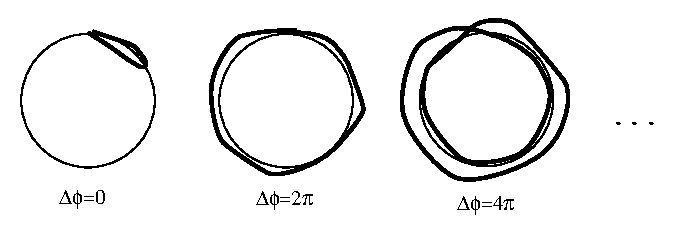
\includegraphics[scale=1.0]{pics/homotopija.eps}}
\end{primjer}
Na ovom skupu klasa krivulja može se prirodno
definirati zbrajanje. Kao reprezentante klasa uzmimo
krivulje koje počnu i završe u nekoj konkretnoj \emph{baznoj} točki, recimo $\phi=0$.
Uzmemo li dvije zatvorene krivulje, njihov zbroj definiramo kao krivulju koja se dobije tako da 
prvo po jednoj krivulji idemo od bazne točke do bazne točke, pa onda
bez "završavanja" nastavimo tako po drugoj i završimo u baznoj točki.
Obzirom na takvo zbrajanje (klasa) krivulja, ovaj skup čini grupu
poznatu pod imenom \emph{fundamentalna grupa} ili \emph{prva grupa homotopija} $\pi_1$. 
Ta grupa je temeljno topološko obilježje svake grupe. Prema gornjem
primjeru vidimo da je $\pi_1\left(\SO{2} \right) = (\mathbb{Z}, +)$.

\begin{primjer}[\SO{3}]
Svaki element grupe \SO{3} se može na jedinstven način definirati
smjerom osi rotacije i iznosom kuta rotacije pa se grupna mnogostrukost
može prikazati kao puna lopta promjera $\pi$ s identificiranim nasuprotnim
točkama njene površine:

\centerline{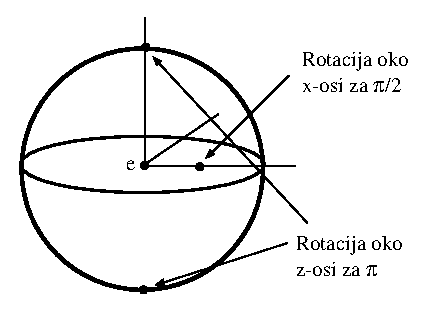
\includegraphics[scale=0.8]{pics/so3mnogostrukost.eps}}

Položaj točke u lopti dan je u sfernom koordinatnom sustavu kao
$(r, \theta, \phi)$. Kutovi $\theta$ i $\phi$ definiraju usmjerenje
osi rotacije, a udaljenost $r \le \pi$ točke od ishodišta definira kut rotacije.
Svaka rotacija je u pozitivnom smjeru. Rotacije oko neke osi za 
kuteve $(\pi, 2\pi)$ se dobiju rotacijom oko
suprotno usmjerene osi. Identifikacija nasuprotnih točaka je posljedica
činjenice da je su rotacije za $\pi$ oko suprotno usmjerenih osi
identične pa tek uz takvu identifikaciju imamo ispravnu bijekciju
između lopte (grupnog prostora) i \SO{3} grupe rotacija. 

Za promatranje
klasa krivulja kao baznu točku možemo uzeti središte lopte. Sve krivulje
koje ostaju u unutrašnjosti lopte se mogu kontinuirano deformirati jedna
u drugu pa pripadaju istoj klasi. Da bi dobili novu klasu promotrimo
krivulju koja dolazi do površine u točki $A$ i onda se nastavlja u unutrašnjost
od antipodne točke $A'$. Naglasimo da je krivulja neprekinuta zahvaljujući
identičnosti $A'=A$.
Kontinuirane deformacije ove krivulje će uvijek
zadržati svojstvo prolaska površinskom točkom (kako se $A$ miče, $A'$ se
miče tako da ostane antipodna) i krivulja se ne može deformirati u krivulje
iz prve klase koje su cijele u unutrašnjosti lopte. Dakle, dobili smo
drugu klasu. Ukoliko sad promotrimo krivulje koje prolaze dvama različitim površinskim
točkama $A$ i $B$, u nadi da ćemo možda dobiti novu klasu, vidimo da je takve
krivulje moguće deformirati do situacije da se točke stope i krivulja potpuno
ubaci u unutrašnjost lopte, kako je prikazano na slici.

\centerline{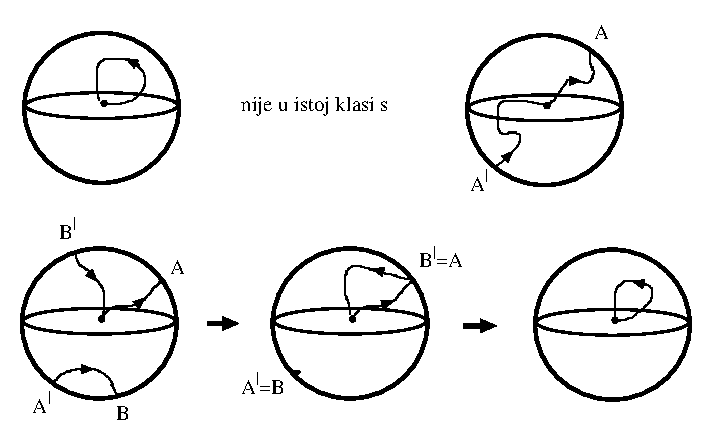
\includegraphics[scale=0.8]{pics/dvostruka_povezanost_so3.eps}}

Tako te krivulje ne čine novu nego pripadaju prvoj klasi.
Krivulja kroz tri površinske točke će se istim postupkom moći deformirati u 
krivulju kroz jednu točku i tako dalje. Dakle, postoje točno dvije klase
krivulja i kažemo da je  \SO{3} \emph{dvostruko povezana}.
Njena prva grupa homotopija je time\footnote{Običaj je grupu $(\{+1, -1\}, \cdot)$
    zvati $\mathbb{Z}_2$ premda bi prema našoj nomenklaturi iz prvog dijela
    knjige konzistentnije bilo zvati je $\mathrm{C}_2$, dok je $\mathbb{Z}_2$
    zapravo $\{0, 1\}$ uz operaciju zbrajanja modulo 2, što se onda prirodno
    generalizira na veće grupe $\mathbb{Z}_n$. No, u svjetlu činjenice da su
    sve grupe reda dva ionako izomorfne, to nije
    prebitno.}
    $\pi_1\left(\SO{3} \right) = \mathbb{Z}_{2} = (\{+1, -1\}, \cdot)$.
\end{primjer}

\begin{primjer}[\SU{2}]
Grupna mnogostrukost od \SU{2} je 3-sfera tj. generalizacija uobičajene
sfere (2-sfere) na četverodimenzionalni prostor. (Vidi vježbe za ovo.)
Može se pokazati da je svaka $n$-sfera s $n>1$ jednostavno povezana.
\secret{Hamermesh, p.320, stereografskom projekcijom se pokazuje
da je $S^n$ bez jedne točke homeomorfan $\mathbb{R}^n$. \emph{``You
cannot lasso a sphere''}}
\end{primjer}

Ako postoji homomorfizam s povezane Lieve grupe G na povezanu Lievu
grupu H s \emph{diskretnom} jezgrom K onda kažemo da grupa G 
\emph{pokriva} grupu H onoliko puta koliko elemenata ima K.
(Prisjetite se teorema \ref{th:izomorfizam} o izomorfizmu.)
Također, Lieve algebre tih grupa su izomorfne.

\begin{primjer}[\SO{3} i \SU{2}]
\SO{3} i \SU{2} su homomorfne. Sam homomorfizam ćemo konstruirati na 
vježbama gdje ćemo vidjeti da je on 2-1 s \SU{2} na \SO{3} tj. jezgra
K ima dva elementa. Dakle \SU{2} pokriva \SO{3} dva puta.
\end{primjer}

\begin{teorem}
Među grupama koje pokrivaju povezanu Lievu grupu G, postoji jedinstvena
grupa koja je jednostavno povezana --- \emph{univerzalna grupa pokrivanja}.
Broj pokrivanja jednak je povezanosti od G. \emph{(Bez dokaza)}
\end{teorem}

Npr. \SU{2} je univerzalna grupa pokrivanja za \SO{3}. Prema
teoremu o izomorfizmu  \SU{2}/$\{1,-1\}$=\SO{3}.\\[1ex]

\centerline{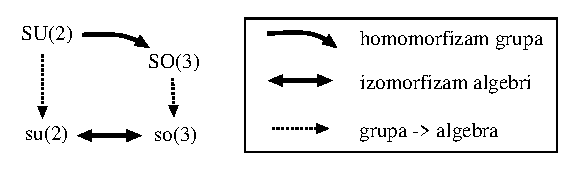
\includegraphics[scale=1.0]{pics/so3pokrivanje.eps}}

Općenita situacija je\\[1ex]

\centerline{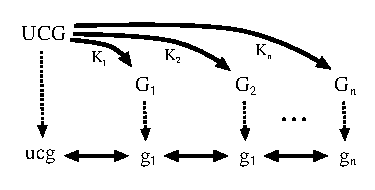
\includegraphics[scale=1.0]{pics/ucg.eps}}

gdje je UCG/$K_i$=G$_i$. Pronalaženjem svih diskretnih invarijantnih
podgrupa od UCG možemo naći sve grupe njoj lokalno izomorfne.


\section{Primjeri Lievih grupa važnih za fiziku}
\label{sec:primjeriLie}

\begin{enumerate}
\item \textbf{Opća linearna grupa}

$\GL{n, \mathbb{C}}$ --- skup svih $n\times n$ regularnih ($\det M \neq 0$)
kompleksnih matrica

Kako je svaka matrica zadana s $n^2$ nezavisnih kompleksnih brojeva, ova
grupa ima $2 n^2$ realnih parametara. Uvjet regularnosti nije ograničenje
koje smanjuje broj parametara, jer je samo riječ o zahtjevu da determinanta,
koja je izraz koji uključuje tih $2 n^2$ parametara bude \emph{različita} od nule.

\begin{equation}
\det M = f(a_1, a_2 , \dots, a_{2n}) \neq 0
\end{equation}

Podgrupa ove grupe je grupa $\GL{n, \mathbb{R}}$ koja očito ima samo
$n^2$ parametara.

\item \textbf{Specijalna linearna grupa}

\begin{equation}
\SL{n, \mathbb{C}} = \{ M\in \GL{n,\mathbb{C}} \; | \; \det M = 1\}
\end{equation}

Ovdje je na svaku matricu postavljen dodatni uvjet
\begin{equation}
\det M = f(a_1, a_2 , \dots, a_{2n}) = 1 \;,
\label{eq:SL}
\end{equation}
koji predstavlja jednu kompleksnu, tj. dvije realne jednadžbe koje
se mogu iskoristiti za eliminaciju dvaju parametera. Tako ova grupa
ima $2 n^2 - 2$ parametra.

Podgrupa ove grupe je grupa $\SL{n, \mathbb{R}}$ koja ima 
$n^2 - 1$ parametar. (Jednadžba (\ref{eq:SL}) je sad samo jedna
realna jednadžba, a ne dvije.)

\item \textbf{Unitarna grupa}

\begin{equation}
U(n) = \{ M\in \GL{n,\mathbb{C}} \; | \; M M^{\dagger} = 1\}
\end{equation}

Prebrojavanje nezavisnih parametara za ovu grupu može se izvesti
na više načina. Uvjet $M M^\dagger = 1$ se može napisati izraženo
preko komponenti matrica kao:
\begin{equation}
\sum_{j=1}^{n} M_{ij} M_{kj}^* = \delta_{ik}\;,
\label{eq:unitaritycondition}
\end{equation}
gdje je iskorišteno $M^{\dagger}_{jk} = M^{*}_{kj}$.
Jednadžba (\ref{eq:unitaritycondition}) predstavlja $n^2$ kompleksnih
jednadžbi ali sve one nisu nezavisne. Promotrimo prvo $n$ jednadžbi
određenih uvjetom $i=k$ (dakle gledamo dijagonalu te matrične jednadžbe):
\begin{equation}
 \sum_j M_{ij} M^{*}_{ij} = \sum_j |M_{ij}|^2 = 1
\label{eq:diagonalcondition}
\end{equation}
To je $n$ realnih jednadžbi koje se mogu upotrijebiti za eliminiranje
$n$ parametara. Dalje možemo gledati jednadžbe određene uvjetom
$i < k$ (dakle gledamo trokut iznad dijagonale matrične jednadžbe).
Te su jednadžbe kompleksne i ima ih $n(n-1)/2$ (broj elemenata u 
spomenutom trokutu). Sve ove jednadžbe su neovisne pa se mogu
iskoristiti za eliminranje $2 \cdot n(n-1)/2 = n(n-1)$ parametara.
Preostaju jednadžbe za $i >k$ (donji trokut matrice), ali kompleksnom
konjugacijom odgovarajućih jednadžbi
\begin{equation}
\sum_{j=1}^{n} M_{ij} M_{kj}^* = 0\;, \qquad i>k
\end{equation}
dobijemo
\begin{equation}
\sum_{j=1}^{n} M_{ij}^* M_{kj}  = \sum_{j=1}^{n} = M_{kj} M_{ij}^* = 0\;, \qquad i>k
\end{equation}
pa uz preimenovanje indeksa $i \leftrightarrow k$
\begin{equation}
\sum_{j=1}^{n} =  M_{ij} M_{kj}^* = 0\;, \qquad k>i
\end{equation}
vidimo da su ove jednadžbe ekvivalentne ovima iz gornjeg trokuta tj. nisu
nezavisne.
Znači sve skupa možemo eliminirati $n + n(n-1) = n^2$ parametara, pa ih
ostane $2n^2 - n^2 = n^2$ što je broj parametara unitarne grupe.
(Drugi način prebrojavanja je da se iskoristi da su retci matrice ortonormirani
vektori. Uvjet normalizacije daje $n$ realnih jednadžbi, a uvjet
ortonogonalnosti $\binom{n}{2}$ kompleksnih, gdje se treba uvjeriti
da odgovarajući zahtjevi na stupce nisu nezavisni od ovih na retke.)

Važno svojstvo unitarnih matrica je da, ukoliko ih interpretiramo kao
operatore nad kompleksnim vektorskim prostorima ($\vec{x} \to M\vec{x}$), 
one čuvaju skalarni produkt
\begin{align}
  (x, y)& = \sum_{i=1}^n x_{i}^* y_i  \longrightarrow
   \sum_{ijk} M^{*}_{ij}x^{*}_j M_{ik}y_{k} \nonumber \\
 & = \text{uvrštavanjem
(\ref{eq:unitaritycondition})} = \sum_{kj} \delta_{kj} x^{*}_j y_k = (x, y)
\label{eq:productinvariance}
\end{align}
Lako je pokazati (D.Z.) da se ovo može uzeti kao alternativna definicija
unitarne grupe tj. da se unitarne matrice mogu definirati kao one koje
čuvaju ovaj skalarni produkt, a onda je svojstvo $M^{\dagger} M = 1$, koje
smo ovdje uzeli kao definiciono, samo posljedica.

\item \textbf{Specijalna unitarna grupa}

\begin{equation}
\SU{n} = \{ M\in U(n) \; | \; \det M  = 1\}
\end{equation}

Za prebrojavanje parametara treba prvo uočiti da je za sve unitarne
matrice determinanta ograničena na apsolutnu vrijednost 1. To slijedi
primjenom Binet-Cauchyjevog teorema na definiciju $M M^{\dagger} = 1$
što daje $|\det M|^2 = 1$ odnostno $\det M = e^{i \phi}$, 
$\phi\in [0, 2\pi)$.
Dodatni uvjet za specijalne unitarne matrice $\det M = 1$ je onda
samo jedna realna jednadžba $\phi = 0$ pa specijalna unitarna grupa
ima točno $n^2 - 1$ parametar.

\item \textbf{Ortogonalna grupa}

\begin{equation}
O(n, \mathbb{C}) = \{ M\in \GL{n,\mathbb{C}} \; | \; M M^{\mathrm{T}} = 1\}
\end{equation}

Kod prebrojavanja uvjeta, jedina razlika obzirom na unitarne matrice
je da umjesto ($i=k$) jednadžbi (\ref{eq:diagonalcondition}) 
koje odgovaraju dijagonali matrične jednadžbe sada imamo
\begin{equation}
 \sum_j M_{ij} M_{ij} = \sum_j M_{ij}^2 = 1
\end{equation}
što su kompleksne jednadžbe pa možemo eliminirati sve skupa
$2n + n(n-1)$ parametara i ostaje ih samo $n(n-1)$.

U fizici se najčešće susrećemo s grupom ortogonalnih \emph{realnih} matrica
\begin{equation}
O(n) \equiv O(n, \mathbb{R}) = \{ M\in \GL{n,\mathbb{R}} \; | \; M M^{\mathrm{T}} = 1\}
\end{equation}
koja ima $n(n-1)/2$ parametara. (Uvjerite se u to.) Ova grupa čuva
kvadratnu formu $\sum_i x_i y_i$ (skalarni produkt na realnom
vektorskom prostoru) što se može upotrijebiti kao alternativna definicija.

\item \textbf{Specijalna ortogonalna grupa}

\begin{equation}
\SO{n, \mathbb{C}} = \{ M\in O(n, \mathbb{C}) \; | \; \det M  = 1\} \;,
\end{equation}
i odgovarajuća realna grupe $\SO{n}$ imaju isti broj parametara kao
$O(n, \mathbb{C})$, odnosno $O(n)$. Naime, uvjet ortogonalnosti
$M M^{\mathrm{T}} = 1$ opet uz primjenu Binet-Cauchyjevog teorema vodi
na $(\det M)^2 = 1$, odnosno
na zaključak da ortogonalne matrice imaju determinantu $\det M = \pm 1$,
pa ograničenje na $\det M = 1$ ne smanjuje dimenziju parametarskog prostora.

\item \textbf{Pseudo-unitarna grupa}

Čine je $n\times n$ matrice
\begin{equation}
U(p, q) = \{ M\in \GL{n,\mathbb{C}} \; | \; M^{\dagger} g M = g\} \;,
\end{equation}
gdje je $p+q=n$ i gdje je $g$ dijagonalna matrica oblika
\begin{equation}
  g = \mathrm{diag}(\underbrace{1, 1, \dots, 1}_{p \times},
\underbrace{-1, -1, \dots, -1}_{q \times}) \;.
\label{eq:metricg}
\end{equation}

Ova grupa ima isti broj parametara kao i $U(n)$, te
čuva kvadratnu formu oblika
\begin{equation}
 \sum_{i=1}^{p} x_{i}^* y_{i} - \sum_{i=p+1}^{p+q=n} x_{i}^* y_i 
\end{equation}
koja nije pozitivno definitna pa nije skalarni produkt u smislu
definicije \ref{def:skalarniprodukt}.


\item \textbf{Pseudo-ortogonalna grupa}

\begin{equation}
O(p, q) = \{ M\in \GL{n,\mathbb{R}} \; | \; M^{\mathrm{T}} g M = g \} \;,
\end{equation}
gdje je $p+q=n$ i gdje je $g$ dijagonalna matrica iz (\ref{eq:metricg}).
Ove matrice čuvaju kvadratnu formu oblika
\begin{equation}
 \sum_{i=1}^{p} x_{i} y_{i} - \sum_{i=p+1}^{p+q=n} x_{i} y_i  \;.
\end{equation}
Najpoznatija grupa ove vrste je grupa Lorentzovih transformacija  $O(1,3)$
(vidi odjeljak \ref{sec:lorentz}).

Specijalnu pseudo-unitarnu grupu $\SU{p,q}$ odnosno specijalnu pseudo-ortogonalnu
grupu $\SO{p,q}$ dobivamo ako se u $U(p,q)$ odnosno $O(p, q)$
ograničimo na matrice s $\det M = 1$.

\end{enumerate}

\subsection{Topološka svojstva Lievih grupa$^*$}

\begin{itemize}
\item $\GL{n, \mathbb{C}}$ je očito nekompaktna (svi elementi matrica
slobodno poprimaju vrijednosti iz skupa $(-\infty, \infty)$ i povezana
(kontinuiranim promjenama elemenata svaku matricu možemo pretvoriti u
jediničnu).

\item $\GL{n, \mathbb{R}}$ je isto nekompaktna. Što se tiče povezanosti,
treba uočiti da je determinanta kontinuirana funkcija elemenata matrice
čija je vrijednost realni broj iz $(-\infty, 0) \cup (0, \infty)$
(zahtjev postojanja inverza isključuje nulu). To znači da kontinuiranim
promjenama parametara ne možemo matrice s negativnim determinantama
pretvoriti u jediničnu i ova grupa ima dvije odvojene komponente povezanosti.

\item Na sličan način možemo zaključiti da grupa $O(n)$, gdje je
determinanta $\pm 1$, isto ima dvije komponenete povezanosti, s time
da je ova grupa kompaktna --- parametri su kutevi rotacija koji poprimaju
vrijednosti iz kompaktnih skupova poput $[0, 2\pi\equiv0)$.
Kad elemente grupe promatramo kao transformacije prostora, elementi
s determinantom $+1$ su čiste rotacije koje se kontinuirano, smanjivanjem
parametra kuta rotacije do nule, mogu povezati s jediničnom transformacijom.
Elementi s determinantom $-1$, osim rotacije uključuju i refleksije pa se
ne mogu kontinuirano povezati s jedinicom.  \label{pag:detO3}

\item $U(n)$ i $\SU{n}$ su kompaktne povezane grupe, gdje je $\SU{n}$ još i
jednostavno povezana.

\item $O(p, q)$ je nekompaktna grupa s četiri komponente povezanosti
što za konkretan primjer grupe $O(1,3)$ pokazujemo u odjeljku \ref{sec:lorentz}.

\end{itemize}

\subsection*{Zadaci za vježbe}

\begin{enumerate}[label=\arabic{chapter}.\arabic*.]

\item \label{zad:O3oSO3} Uvjerite se da je kvocijentna grupa $\O{3}/\SO{3} = \mathrm{C}_{2}$.

\item \label{zad:LeviCivitaProperties} Pokažite da Levi-Civita tenzor ima slijedeća svojstva:
\begin{align*}
\tag{a}\epsilon_{ijk}\epsilon_{imn}&=\delta_{jm}\delta_{kn}-\delta_{jn}\delta_{km}\\
\tag{b}\epsilon_{ijk}\epsilon_{ijm}&=2\delta_{km} \\
\tag{c}\epsilon_{ijk}\epsilon_{ijk}&=6 \\
\tag{d}\epsilon_{ijk}a_j b_k &= (\vec{a}\times\vec{b})_i  \\
\tag{e}\frac{1}{3!}\epsilon_{lmn} \epsilon_{ijs} A_{li} A_{mj} A_{ns} &= \det A
\end{align*}

\item Uporabom svojstava Levi-Civita tenzora pokažite da je
za vektore $\vec{a}$, $\vec{b}$ i \vec{c}
\begin{displaymath}
    \vec{a}\times(\vec{b}\times\vec{c})=(\vec{a}\cdot\vec{c})\vec{b}
 -(\vec{a}\cdot\vec{b})\vec{c}
\end{displaymath}
\secret{Za slične stvari vidi Evett, Am. J. Phys \textbf{34} (1966) 503.}

\item Pokažite da Paulijeve matrice imaju slijedeća svojstva:
\begin{align*}
\tag{a} \sigma_{i}^2 &= 1 \\
\tag{b} \sigma_{i}^\dagger &= \sigma_i \\
\tag{c} \det \sigma_i &= -1 \\
\tag{d} \Tr \sigma_i &=0 \\
\tag{e} [\sigma_i, \sigma_j] &= 2 i \epsilon_{ijk} \sigma_k \\
\tag{f} \{\sigma_i, \sigma_j\}\equiv \sigma_i\sigma_j + \sigma_j \sigma_i &= 2
\delta_{ij} 1 \\
\tag{g} \Tr (\sigma_i \sigma_j) &= 2\delta_{ij} \\
\tag{h} \sigma_i \sigma_j &= \delta_{ij} 1 + i \epsilon_{ijk}\sigma_k\\
\tag{i} e^{-\frac{i}{2}\vec{\sigma}\cdot\unitn \theta} &=
\cos \frac{\theta}{2}-i\vec{\sigma}\cdot\unitn \sin\frac{\theta}{2} \quad\in \SU{2}
\end{align*}

\item \label{zad:abelovaalgebra} Za Abelovu grupu vrijedi $g_1 g_2 g_{1}^{-1} g_{2}^{-1} = e$,
    gdje se objekt $g_1 g_2 g_{1}^{-1} g_{2}^{-1}$ naziva \emph{komutator} elemenata grupe.
    Ako je $g_1$ generiran elementom algebre $g_1 = e^{s X}$, a $g_2 = e^{t Y}$, gdje su
    $s$ i $t$ realni parametri, pokažite da je
\begin{equation}
\frac{\partial^2}{\partial s \, \partial t} \bigg|_{s=t=0} \big( \exp(sX) \exp(tY)
\exp(-sX) \exp(-tY) \big) = [X, Y] \,,
\end{equation}
i time da je algebra $\calA$ Abelove grupe trivijalna $[X, Y] = 0$, za svake $X, Y \in \calA$.

\item Provjerite eksplicitno BCH formulu do kubičnog člana.

\item Pokažite da je grupa \SU{2} homomorfna grupi \SO{3} i da je homomorfizam
       2 na 1 (dvama elementima iz \SU{2} je pridružen jedan element iz \SO{3}).

\item Pokažite da je grupna mnogostrukost grupe \SU{2} hipersfera u
 četverodimenzionalnom prostoru (tzv. \emph{3-sfera}) definirana
 jednadžbom 
\begin{displaymath}
x^2+y^2+r^2+s^2=1 \;.
\end{displaymath}

\item Pokažite da je $(\mathbb{R}, +)$ 
 univerzalna grupa pokrivanja za grupu \SO{2}.

\item Pokažite da matrice
\begin{equation}
 M(\theta) = \begin{pmatrix}
\cosh\theta & \sinh\theta  \\
\sinh\theta & \cosh\theta
\end{pmatrix}
\end{equation}
djelujući na vektore $(x, y)$ čuvaju formu $x^2 - y^2$, te da 
je $\det M(\theta) = 1$, tako da $M(\theta)$ tvore grupu
$\SO{1,1}$.
\end{enumerate}

%Fancy RCS footer:
     \fancyfoot[C]{\texttt{6\_rotacije.tex}}
     \fancyfoot[RO,LE]{\mbox{$$Revision: 1.10 $$}}
     \fancyfoot[LO,RE]{\mbox{$$Date: 2012-02-24 $$}}
% Correcting the title chapter page
\fancypagestyle{plain}{%
    \fancyhf{}
    \fancyhead[RO,LE]{\bfseries \thepage}
    \fancyhead[CO]{\rightmark}
    \fancyhead[CE]{\leftmark}
     \fancyfoot[C]{\texttt{6\_rotacije.tex}}
     \fancyfoot[RO,LE]{\mbox{$$Revision: 1.10 $$}}
     \fancyfoot[LO,RE]{\mbox{$$Date: 2012-02-24  $$}}
    \renewcommand{\headrulewidth}{0.4pt}
    \renewcommand{\footrulewidth}{0.4pt}}

\chapter{Rotacije i moment impulsa u kvantnoj mehanici}
\label{ch:rotacije}

\section{Ireducibilne reprezentacije grupe SO(2)}

Teorija reprezentacija za kompaktne grupe je drastično različita
 od one za nekompaktne grupe

 \emph{Kompaktne} Lieve grupe su one čiji parametri poprimaju
   vrijednosti iz zatvorenih konačnih intervala:\footnote{
  Pojam kompaktnosti općenito zna biti vrlo netrivijalan, ali za
   naše Lieve grupe koje su \emph{linearne} tj. posjeduju barem
   jednu vjernu konačnodimenzionalnu reprezentaciju vrijedi ova
 pojednostavljena definicija.}
\begin{displaymath}
         p \in [a, b]\;,  \quad a,b\neq \pm \infty
\end{displaymath}

\textbf{Primjeri:}
\begin{itemize}
\item grupa translacija nije kompaktna jer parametri translacije
      nisu ograničeni: $p \in (-\infty, \infty)$
\item Lorentzova grupa nije kompaktna jer parametar Lorentzovog
      potiska dolazi iz otvorenog intervala: $v \in [0,c)$
\item grupa SO(2) je kompaktna: $\phi\in[0, 2\pi=0]\equiv[0,2\pi)$
\item grupa SO(1,1) nije kompaktna
\end{itemize}

Ključna prednost kompaktnosti je činjenica da su kontinuirane funkcije
na kompaktnom skupu integrabilne pa 
velik broj teorema o konačnim grupama vrijedi i za kompaktne Lieve
grupe, uz zamjenu (u dokazima i iskazima):
\begin{displaymath}
    \frac{1}{n} \sum_{g} \longrightarrow \int \rmd g \;,
\end{displaymath}
gdje integral, zahvaljujući kompaktnosti, konvergira.

- Mjeru integrala treba izabrati tako da vrijedi
\begin{displaymath}
  \int dg f(g) = \int dg f(hg) = \int dg f(gh) \quad \forall h \in G \;.
\end{displaymath}
Integraciju koja ima to svojstvo zovemo \emph{invarijantna}.  
Takvo nam je svojstvo
trebalo za dokaze teorema o reprezentacijama. Uvijek je moguće izabrati
mjeru tako da integracija bude invarijantna.

- Tako možemo ``preuzeti'' iz teorije reprezentacije konačnih grupa
  teorem da su sve reprezentacije ekvivalentne unitarnima. (To nam
 je važno jer je unitarnost željeno svojstvo transformacija kvantnomehaničkih
 stanja.)

- Specijalno, svi IRREPSi od SO(2) su ekvivalentni unitarnima, pa se,
  kao što smo to radili i kod konačnih grupa, smijemo ograničiti na
  unitarne IRREPSe bez gubitka općenitosti. 

- SO(2) je Abelova $\imp$ svi IRREPsi su 1D, što uz unitarnost 
($uu^\dagger = uu^* = |u|^2=1$) znači:
\begin{displaymath}
D(\phi)=e ^{-i f(\phi)} \;,  f(\phi) \in \mathbb{R} \;.
\end{displaymath}

Zahtjev homomorfnosti s grupom rotacija, koja je aditivna, dalje
povlači
\begin{displaymath}
   f(\phi_1)+f(\phi_2) = f(\phi_1+\phi_2)
\end{displaymath}
što znači da je $f(\phi)=m\phi$, $m\in\mathbb{R}$.
Na kraju, zahtjev periodičnosti daje:

- $D^{(m)}(\phi)=D^{(m)}(\phi + 2\pi) \imp m \in \mathbb{Z}$

- Dakle, imamo prebrojivo beskonačno 1D IRREPsa, i označavamo
  ih cijelim brojem $m$.

- Karakteri: $\chi^{(m)}(\phi)=D^{(m)}(\phi)=e^{-\rmis m \phi}$

- Ortogonalnost:
\begin{displaymath}
(\chi^{(m)}, \chi^{(m')})=\int_{0}^{2\pi}\frac{\rmd \phi}{2\pi}\,
 e^{\rmis m \phi}e^{-\rmis m' \phi} = \delta_{mm'}
\end{displaymath}

- (D.Z. Uvjerite se da je ovakva integracija invarijantna u gornjem smislu.)


- Koeficijenti u razvoju direktnog produkta dvaju IRREPsa:
\begin{displaymath}
  \Gamma^{(m)}\otimes\Gamma^{(n)} =
  \sum \oplus\: a_{k}\Gamma^{(k)} 
\end{displaymath}
\begin{eqnarray*}
a_{k} & = & (\chi^{(k)}, \chi^{(m)}\chi^{(n)}) \\
      & = & \int_{0}^{2\pi}\frac{\rmd \phi}{2\pi}\,
    e^{\rmis k \phi}e^{-\rmis m \phi}e^{-\rmis n \phi} = \delta_{k,m+n}
\end{eqnarray*}
tj.
\begin{displaymath}
  \Gamma^{(m)}\otimes\Gamma^{(n)} =
  \sum_{k} \oplus\: \delta_{k,m+n}\Gamma^{(k)} = \Gamma^{(m+n)}
\end{displaymath}

- Rastav reducibilne reprezentacije:
\begin{displaymath}        
 D_{\rm 2D} (\phi) = \left( 
\begin{array}{cc}        
\cos\phi & -\sin\phi \\
\sin\phi & \cos\phi
\end{array}                
\right) \qquad \chi_{\rm 2D}=2\cos\phi
\end{displaymath}
\begin{eqnarray*}
a_k & = & (\chi^{(k)}, \chi_{\rm 2D}) \\
    & = & \int_{0}^{2\pi}\frac{\rmd \phi}{2\pi}\,
   e^{\rmis k \phi} 2\cos\phi  \\
 & = & \int_{0}^{2\pi}\frac{\rmd \phi}{2\pi}\,
  e^{\rmis k \phi} ( e^{\rmis  \phi} + e^{-\rmis  \phi}) \\
 & = & \delta_{k,-1} + \delta_{k, 1}
\end{eqnarray*}
Znači postoji $S$ [pronađite za D.Z.] takva da
\begin{displaymath}
  S D_{\rm 2D} (\phi) S^{-1} = \left(
\begin{array}{cc}        
e^{\rmis  \phi} &  0 \\
0 & e^{- \rmis  \phi}
\end{array}                
\right) 
\end{displaymath}

\subsubsection*{Digresija: Projektivne reprezentacije$^*$}

- U QM postoje sustavi za koje $m = 1/2, 3/2, 5/2, \ldots$ tj.
  $D^{(m)}(\phi)=-D^{(m)}(\phi + 2\pi)$


Po definiciji, reprezentacija $\Gamma=\{D(\phi)\}$ grupe G mora zadovoljavati:
\begin{displaymath}
    D(\phi_1)D(\phi_2)=D(\phi_1\circ_{\textrm{\tiny G}}\phi_2)
        =D(\phi_1 + \phi_2)
\end{displaymath}
dok za $m = 1/2, 3/2, 5/2, \ldots$ imamo npr.
\begin{displaymath}
 D(\pi) D(\pi) = e^{i m \pi}e^{i m \pi} = e^{2 i m \pi}=-1
\neq D(2\pi)=1 \;.
\end{displaymath}
Riječ je o tome da se u QM $D(\phi_1)D(\phi_2)\ket{\alpha}$ i
$D(\phi_1 + \phi_2)\ket{\alpha}$ smiju razlikovati za fazu
a da i dalje opisuju isto fizikalno stanje.

Tako na QM stanjima dopuštamo reprezentiranje grupe i tzv.
\emph{projektivnim reprezentacijama} s ``olabavljenim'' uvjetom homomorfizma:
\begin{displaymath}
   D(g_1)D(g_2)=e^{i \phi(g_1,g_2)}D(g_1 g_2) \;.
\end{displaymath}

- O grupi ovisi hoće li ona imati i projektivnih REP, a o fizikalnom
sustavu hoće li se transformirati obzirom na projektivne REP ili ne.

- Jedan od načina da grupa ima i projektivne reprezentacije je da
  ne bude jednostavno povezana.

SO(3) je dvostruko povezana i dopušta dvije faze: $\pm 1$. Fermioni
su čestice koje se transformiraju projektivno.

SO(2) je beskonačno povezana i ima beskonačno mogućih faza. No, sustavi
koje razmatramo su 3D i čak i pod 2D rotacijama mogu samo promijeniti
predznak tj. SO(2) je ovdje samo podgrupa od SO(3).

\section{Ireducibilne reprezentacije grupe SO(3) tj. SU(2)}

- Grupa SO(3) nije Abelova i IRREPSi više nisu 1D pa konstrukcija nije
tako laka kao za SO(2).

- Lakše je konstruirati reprezentacije SO(3) \emph{algebre}, a onda
  eksponencijacijom dobiti reprezentacije grupe.

- Algebru čine tri generatora grupe, $X_1, X_2, X_3$, eksplicitno navedena u
(\ref{eq:SO3generators}), sa komutacijskim relacijama
\begin{equation}
          [X_i, X_j] = \epsilon_{ijk} X_k
\end{equation}
ali mi ćemo raditi s malo drugačije izraženom algebrom, preko kvantnomehaničkih operatora
momenta impulsa, $J_1, J_2, J_3$, $J_i=\rmi \hbar X_i$ koji zadovoljavaju
\begin{equation}
          [J_i, J_j] = i \hbar \epsilon_{ijk} J_k
\label{eq:SU2algebra}
\end{equation}
 
Elementi grupe su $e^{\phi\unitn\cdot\vec{X}}=e^{(-i/\hbar)\phi\unitn\cdot
 \vec{J}}$ što se slaže sa odjeljkom \ref{sec:lievealgebre}.

- Iz unitarnosti reprezentacije ondmah slijedi da su $J_i$ hermitski, kao
  što i treba biti. Znači da su njihove svojstvene vrijednosti realne.

- Operator $\vec{J}^2 = J_{x}^2 + J_{y}^2 + J_{z}^2$ je Casimirov
  (cf. odjeljak 4.2) tj. komutira sa svim elementima algebre:
\begin{equation}
   [\jsq, J_{i}^2]=0\;, \quad i=1,2,3
\end{equation}

- Kako nas zanimaju IRREPSi, iz druge Schurove leme slijedi da $\jsq$
mora biti proporcionalan jediničnom operatoru: $\jsq \propto \Eins$.
Tako se svojstvena vrijednost od $\jsq$ ne mijenja kroz cijelu IRREP i
zgodna je za njeno označavanje. Usporedimo sad IRREPse grupe rotacija
na običnom 3D prostoru i na prostoru kvantnomehaničkih stanja.

\begin{itemize}
\item  IRREP na 3D euklidskom prostoru:
\begin{displaymath}
   D^{(3D)}_{ij}(\unitn, \phi) r_j = \text{lin. komb. od}\: \hat{x}, \hat{y}, \hat{z}
\end{displaymath}
   $\unitn, \phi$ --- parametri \\
  $3D$ --- oznaka IRREPsa \\
  $r_j$ --- koordinate vektora $r_x, r_y, r_z$

\item IRREPsi rotacija na Hilbertovom prostoru:
\begin{displaymath}
   D^{(\beta)}(\unitn,\phi) \ket{\beta, m} =
 e^{(-i/\hbar)\vec{J}\cdot\unitn\phi}\ket{\beta, m} =
\text{lin. komb. od}\: \ket{\beta, m_1}, \ket{\beta, m_2}, \dots
\end{displaymath}
$\beta$ --- indeks IRREPsa (na $\vec{J}$ često implicitan, no
 ponekad se piše $\vec{J}^{(\beta)}$) \\
$ m $ --- ``koordinata'' koja razlikuje vektore unutar istog IRREPsa.\\
 Vektori baze prostora na koji djeluje IRREP $\beta$ su definirani slijedećim
relacijama:
\begin{eqnarray}
  \jsq \ket{\beta, m} &=& \beta \hbar^2 \ket{\beta, m} \;.  \\
  J_z \ket{\beta, m} &=& m \hbar \ket{\beta, m} \;.
\end{eqnarray}
\end{itemize}

Sada ćemo eksplicitno konstruirati IRREPse od $SU(2)$, koristeći
isključivo komutacijske relacije (\ref{eq:SU2algebra}).
\secret{Ova konstrukcija se radi na kvantnoj pa se može
preskočiti i samo rekapitulirati sažetak na kraju ovog odjeljka.}
Prvo definiramo operatore \emph{podizanja i spuštanja}
\begin{displaymath}
    J_{\pm} = J_x \pm i J_y \;, \qquad [\jsq, J_\pm] =0
\end{displaymath}
 
\begin{eqnarray*}
 [J_z, J_\pm]& = & [J_z, J_x] \pm i [J_z, J_y] = i\hbar J_y \pm i (-i\hbar J_x)
 \\ & = & \pm \hbar (J_x \pm i J_y) = \pm \hbar J_\pm
\end{eqnarray*}

Slično (pokažite):
\begin{displaymath}
 [J_+, J_-] = 2 \hbar J_z
\end{displaymath}

 Djelovanjem ovih operatora dizanja i spuštanja na vektore neke IRREP,
ostajemo naravno u toj istoj IRREP:
\begin{displaymath}
   \jsq(J_{\pm}\ket{\beta, m})=J_{\pm}\jsq\ket{\beta, m}=\beta\hbar^2
    (J_{\pm}\ket{\beta, m}) \;,
\end{displaymath}
ali svojstvena vrijednost od $J_z$ se mijenja:
\begin{equation}
J_z(J_{\pm}\ket{\beta, m})=([J_z,J_{\pm}]+J_{\pm}J_z)\ket{\beta, m}=
\hbar(m\pm 1)J_{\pm}\ket{\beta, m} \;,
\label{jzjpm}
\end{equation}
tj.
\begin{displaymath}
    J_{\pm}\ket{\beta, m}\propto \ket{\beta, m\pm 1} \;.
\end{displaymath}


Do kuda  može ići to dizanje i spuštanje tj. koliko različitih vrijednosti
može poprimiti $m$?

Tvrdnja: $m^2 \leq \beta$

Dokaz: $J_{\pm}^{\dagger}=J_{\mp}$, jer $J^{\dagger}_{x,y,z}=J_{x,y,z}$.
\begin{eqnarray*}
 \frac{1}{2}(J_+ J_{+}^{\dagger} + J_{+}^{\dagger}J_+)& = &
 \frac{1}{2}(J_+ J_{-}+ J_- J_+) \\
& = & \frac{1}{2} \left[ (J_x + i J_y)(J_x - i J_y) + \textrm{h. c.} \right]
\\ & = & \frac{1}{2} \left[ J_{x}^2 + i J_y J_x - i J_x J_y + J_{y}^2
  + J_{x}^2 - i J_y J_x + i J_x J_y + J_{x}^2 \right] \\
& = & J_{x}^2 + J_{y}^2 = \jsq - J_{z}^2
\end{eqnarray*}
No,
\begin{displaymath}
\bra{\beta, m}J_{+}^{\dagger}J_+ \ket{\beta, m} =
\bra{J_{+}\beta, m}J_{+}\beta, m\rangle  \geq 0 \quad \textrm{i isto za}
J_+ J_{+}^{\dagger}
\end{displaymath}
Slijedi da je
\begin{displaymath}
\bra{\beta, m}(\jsq - J_{z}^2)\ket{\beta, m}=
\bra{\beta, m}(\beta\hbar^2 - m^2\hbar^2)\ket{\beta, m} =
(\beta - m^2)\hbar^2 \geq 0
\end{displaymath}
Q.E.D.

Dakle, za svaki $\beta$ postoji $m_{\textrm{\scriptsize max}}$ tako da 
\begin{displaymath}
 J_+ \ket{\beta, m_{\textrm{\scriptsize max}}} = 0
\end{displaymath}
(To je jedini način da (\ref{jzjpm}) ostane vrijediti.)

$m_{\textrm{\scriptsize max}}(\beta)$=?

\begin{displaymath}
J_- J_+ \ket{\beta, m_{\textrm{\scriptsize max}}} = 0
\end{displaymath}
\begin{eqnarray*}
J_- J_+ =(J_x - i J_y)(J_x - i J_y)
   & = &J_{x}^2 + J_{y}^2 +i (J_x J_y - J_y J_x) \\
 & = & J_{x}^2 + J_{y}^2 - \hbar J_z \\
 & = & \jsq - J_{z}^2 - \hbar J_z
\end{eqnarray*}
Pa je
\begin{displaymath}
 (\jsq - J_{z}^2 - \hbar J_z)\ket{\beta, m_{\textrm{\scriptsize max}}}
 = (\beta\hbar^2 - m_{\textrm{\scriptsize max}}^2 \hbar^2 
                 - m_{\textrm{\scriptsize max}}   \hbar^2 )
\ket{\beta, m_{\textrm{\scriptsize max}}} = 0 \;,
\end{displaymath}
pa kako $\ket{\beta, m_{\textrm{\scriptsize max}}}$ nije nul-vektor
slijedi da je
\begin{displaymath}
    \beta = m_{\textrm{\scriptsize max}} ( m_{\textrm{\scriptsize max}} +1)\;.
\end{displaymath}

Iz maločas dokazane činjenice da je $m^2 \le \beta$ slijedi također
da ni spuštanje vrijednosti $m$ operatorom spuštanja ne može ići
unedogled već da mora postojati $m_{\textrm{\scriptsize min}}$
sa svojstvom
\begin{displaymath}
    J_- \ket{\beta, m_{\textrm{\scriptsize min}}} = 0 \;,
\end{displaymath}
iz čega postupkom analognim ovom gore dolazimo do
\begin{displaymath}
    \beta = m_{\textrm{\scriptsize min}} ( m_{\textrm{\scriptsize min}} -1)\;.
\end{displaymath}

Izjednačivši ove dvije vrijednosti za $\beta$ 
\begin{displaymath}
            m_{\textrm{\scriptsize max}} ( m_{\textrm{\scriptsize max}} +1)
= m_{\textrm{\scriptsize min}} ( m_{\textrm{\scriptsize min}} -1)
\end{displaymath}
dobijemo kvadratnu jednadžbu za $m_{\textrm{\scriptsize min}}$ od čija
dva rješenja $m_{\textrm{\scriptsize min}}=m_{\textrm{\scriptsize max}}+1$
i $m_{\textrm{\scriptsize min}} = - m_{\textrm{\scriptsize max}}$ ovo
prvo ne dolazi u obzir jer je $m_{\textrm{\scriptsize max}}$ po pretpostavci
najveća moguća vrijednost za $m$. Tako imamo, uvodeći oznaku
$j=m_{\textrm{\scriptsize max}}$,
\begin{displaymath}
               -j = m_{\textrm{\scriptsize min}} \le m \le 
 m_{\textrm{\scriptsize max}} = j   \;.
\end{displaymath}

Nadalje, kako operatori $J_\pm$ dižu ili spuštaju $m$ točno za 1, mora
biti $m_{\textrm{\scriptsize max}} = m_{\textrm{\scriptsize min}} +n $,
gdje je $n\in \mathbb{N}_{0}$, tj. $j = -j +n  \imp j=n/2$
\begin{displaymath}
  j= 0, \frac{1}{2}, 1, \frac{3}{2}, 2, \ldots \;.
\end{displaymath}

  Vrijednost $\beta = j(j+1)$ je ista za cijelu IRREP i uobičajenije
je upravo $j$ koristiti za označavanje IRREPa:
\begin{displaymath}
  \ket{\beta, m} \longrightarrow \ket{j, m} \;,
\end{displaymath}
gdje $m$ poprima vrijednosti
\begin{displaymath}
   m= -j, -j+1, \ldots, j-1, j
\end{displaymath}
i gdje vektori baze IRREPa $\ket{j, m}$ zadovoljavaju
\begin{eqnarray*}
 \jsq \ket{j, m}& = & \hbar^2 j(j+1)\ket{j, m} \quad \mbox{i} \\
 J_z \ket{j, m} & =  &\hbar m \ket{j, m} \;.
\end{eqnarray*}
Tako smo koristeći isključivo komutacijske relacije algebre grupe rotacija
konstruirali sve njene ireducibilne reprezentacije!

Kako je ta algebra zajednička i grupi $SO(3)$ i grupi $SU(2)$ dobili
smo i reprezentacije s polucjelobrojnim momentom impulsa $j$.

Još nas zanima i točno djelovanje operatora $J_\pm$ na vektore baze:
\begin{displaymath}
     J_+ \ket{j, m} = c_{jm} \ket{j, m+1} \;.
\end{displaymath}
Zahvaljujući ortonormiranosti:
\begin{eqnarray*}
 |c_{jm}|^2 & = & \bra{j, m} J_- J_+ \ket{j, m} \\
            & = & \bra{j, m}(\jsq - J_{z}^2 - \hbar J_z \ket{j, m} \\
& = & \bra{j, m}(\hbar^2 j(j+1) - \hbar^2 m^2 - \hbar^2 m \ket{j, m}  \\
            & = & \hbar^2[j(j+1)-m(m+1)] \\
            & = & \hbar^2 (j-m)(j+m+1)
\end{eqnarray*}
Faza od $c_{jm}$ je neodređena i prema tzv. Condon-Shortley konvenciji
odabire se realan i pozitivan $c_{jm}$:
\begin{displaymath}
  J_+ \ket{j, m} = \hbar \sqrt{(j-m)(j+m+1)} \ket{j, m+1} \;.
\label{jplus}
\end{displaymath}
Slično, [pokažite]
\begin{displaymath}
  J_- \ket{j, m} = \hbar \sqrt{(j+m)(j-m+1)} \ket{j, m-1} \;.
\label{jminus}
\end{displaymath}

Ove relacije nam omogućuju da odredimo matrične elemente operatora
momenta impulsa između proizvoljnih stanja. Također, eksponencijacijom
možemo odrediti matrične elemente samih operatora rotacija:
\begin{displaymath}
    \bra{j,m'} D^{(j)}(\hat{\vec{n}},\phi) \ket{j, m} \quad - \quad
\text{Wignerove D-funkcije}
\end{displaymath}
Za konkretne primjere vidi vježbe.

\textbf{Sažetak:}

\begin{itemize}
\item  Operatori momenta impulsa $J_x, J_y$ i $J_z$ te njihove kombinacije
$\jsq, J_\pm, \ldots$ za dani $j$, tj. za danu ireducibilnu reprezentaciju
grupe rotacija, djeluju na ($2j+1$)-dimenzionalnom vektorskom prostoru
razapetom vektorima $\ket{j, m}$, $m=-j, -j+1, \ldots, j-1, j$.

\item operatori $D^{(j)}=e^{-i \vec{J}\cdot\unitn\phi/\hbar}$ čine
  reprezentaciju grupe rotacija na ($2j+1$)-dimenzionalnom  Hilbertovom
  vektorskom prostoru kvantnomehaničkih stanja

\item $J_{\pm}$ povezuju svih $2j+1$ vektora $\ket{j, m}$ tj.
  reprezentacija je stvarno ireducibilna

\item baza vektorskog prostora $\ket{j, m}$, $m=-j, -j+1, \ldots, j-1, j$ 
 se obično naziva \emph{multiplet}. (Neki autori tako zovu cijeli
 vektorski prostor.)
  \begin{itemize}
\item  $j=0$ : \emph{singlet}
\item  $j=\frac{1}{2}$ : \emph{dublet}
\item  $j=1$ : \emph{triplet}
\item  $\cdots$ 
\end{itemize}
\end{itemize}

\textbf{Orbitalni moment impulsa:}

- Specijalna vrsta momenta impulsa koja je oblika $\vec{L} = \vec{r}
  \times \vec{p}$

- Kao posljedica toga (ne sasvim trivijalna \secret{cf. Kaplan and Wu, 
Chinese J. of Phys. \textbf{9} (1971) 31; Gatland, Am. J. Phys.
\textbf{74} (2006) 191.}), svojstvene vrijednosti su 
 isključivo  cjelobrojne:
\begin{displaymath}
     \vec{L}^2 \ket{l, m} = \hbar^2 l(l+1) \ket{l,m} \qquad l=0,1,2,\ldots
\end{displaymath}
i označavaju se s $l$, a ne $j$.

- Iz povijesnih razloga vezanih uz atomsku fiziku, stanja s $l=0,1,2,\ldots$
se često nazivaju $S, P, D,\ldots$ stanja, a $m$ se ponekad naziva
\emph{magnetski} kvantni broj (zbog svoje uloge u Zeemanovom efektu).

\section{Zbrajanje momenata impulsa i Clebsch-Gordanovi koeficijenti}

Sustav od dvije čestice, sa spinovima $j_1$ i $j_2$ u stanju 
$\ket{j_1, m_1; j_2, m_2}$ ima svojstva:
\begin{align*}
\vec{J}_{1}^2 \ket{j_1, m_1; j_2, m_2} &= j_1(j_1+1)\hbar^2 
  \ket{j_1, m_1; j_2, m_2} \\
\vec{J}_{2}^2 \ket{j_1, m_1; j_2, m_2} &= j_2(j_2+1)\hbar^2 
  \ket{j_1, m_1; j_2, m_2} \\
J_{1z}\ket{j_1, m_1; j_2, m_2} &= m_1 \hbar \ket{j_1, m_1; j_2, m_2}\\
J_{2z}\ket{j_1, m_1; j_2, m_2} &= m_2 \hbar \ket{j_1, m_1; j_2, m_2}
\end{align*}
\begin{align*}
\ket{j_1, m_1} &\in V_1\\
\ket{j_2, m_2} &\in V_2\\
\ket{j_1, m_1; j_2, m_2}&\equiv\ket{j_1, m_1}\ket{j_2, m_2} \in V_1\otimes V_2
\end{align*}
Na vektorskom
prostoru $V_1$ grupa rotacija reprezentirana je operatorima $D^{(j_1)}=
\exp(-i\vec{J}_1\cdot\hat{\vec{n}}\theta/\hbar)$ (i slično za $V_2$),
a na $V_1\otimes V_2$ operatorima
$D^{(j_1)}\otimes D^{(j_2)}$.

Međutim, $D^{(j_1)}\otimes D^{(j_2)}$ je općenito reducibilna reprezentacija
koja nema dobro definiran spin. $\ket{j_1, m_1; j_2, m_2}$ nije nužno svojstveno
stanje od $\vec{J}^2 = (\vec{J}_1 + \vec{J}_2)^2$ --- operatora ukupnog spina
sustava.

Rastav na IRREPSE:
\begin{displaymath}
  D^{(j_1)}\otimes D^{(j_2)} =
  \sum_J \oplus\: a_{J}D^{(J)} \quad
   \textrm{ - Clebsch-Gordanov razvoj }
\end{displaymath}

\begin{displaymath}
a_J = \left( \chi^{(J)}, \chi^{(j_1)} \chi^{(j_2)} \right)
\end{displaymath}

Za općeniti račun skalarnih umnožaka karaktera trebali bismo
znati invarijantno integrirati u grupnom prostoru (cf. Jones,
Appendix C ili Hamermesh 9-2), ali ovdje ćemo potrebni rezulatat
dobiti i bez toga, uz par matematičkih trikova:

Kao reprezentante klasa biramo rotacije oko $z$-osi.
\begin{equation}
\begin{split}
 \chi^{(j)}(\phi) &= \Tr D^{(j)}(\phi) = \Tr e^{(-i/\hbar)J_3 \phi} \\
 &= \Tr \textrm{diagonal}\left( e^{-i j\phi }, e^{-i (j-1)\phi}, \ldots,
e^{-i(-j)\phi}\right)\\
&= e^{-ij\phi } + e^{-i (j-1)\phi} + \cdots + e^{-i(-j)\phi}\\
&= \text{geom. red s omjerom članova $e^{i j\phi}$} \\
&= e^{-i j\phi} \frac{1- (e^{i j\phi})^{2j+1}}{1-e^{i\phi}}
= \frac{e^{-i(j+1/2)\phi} - e^{i(j+1/2)\phi}}{e^{-i\phi/2}-e^{i\phi/2}}\\
&= \frac{\sin(j+1/2)\phi}{\sin\phi/2}
\end{split}
\end{equation}


Odredimo sada koeficijente $a_J$ Clebsch-Gordanovog razvoja. Pretpostavimo
prvo da je $j_1 \ge j_2$.
\begin{equation}
\begin{split}
\chi^{(j_1)}(\phi)\chi^{(j_2)}(\phi)&=
 \frac{e^{+i(j_1+1/2)\phi} - e^{-i(j_1+1/2)\phi}}{2i\sin\phi/2}
\sum_{m=-j_2}^{j_2}e^{i m \phi}\\
&= \frac{1}{2 i \sin\phi/2} \sum_{m=-j_2}^{j_2}
\left[ e^{i(j_1+m+1/2)\phi} - e^{-i(j_1-m+1/2)\phi}\right]\\
&= (\text{zamjena $m\to -m$ u drugom članu}) \\
&=\sum_{m=-j_2}^{j_2} \frac{\sin(j_1+m+1/2)\phi}{\sin\phi/2}\\
&=\sum_{m=-j_2}^{j_2} \chi^{(j_1 + m)}(\phi) \qquad (J\equiv j_1 +m) \\
&=\sum_{J=j_1-j_2}^{J=j_1+j_2} \chi^{(J)}(\phi) \;.
\end{split}
\end{equation}
($J$ mora biti pozitivan da bi bio labela neke IRREPS. Zato smo
tražili $j_1\ge j_2$.)
Za slučaj $j_2 \ge j_1$ imali bi sve isto, uz zamjenu $j_1 \leftrightarrow
j_2$. Slijedi da općenito možemo pisati:
\begin{displaymath}
 \chi^{(j_1)}(\phi)\chi^{(j_2)}(\phi)=
\sum_{J=|j_1-j_2|}^{J=j_1+j_2} \chi^{(J)}(\phi)
\end{displaymath}
Dakle,
\begin{displaymath}
 a_J = \left(\chi^{(J)}, \chi^{(j_1)}\chi^{(j_2)}\right) =
 \sum_{J'=|j_1-j_2|}^{J'=j_1+j_2} 
\underbrace{\left(\chi^{(J)}, \chi^{(J')}\right)}_{\delta_{JJ'}}
\end{displaymath}
odnosno,
\begin{equation}
D^{(j_1)} \otimes D^{(j_2)} = \sum_{J=|j_1-j_2|}^{J=j_1+j_2} 
\oplus D^{(J)}
\end{equation}

Npr. $D^{(1/2)}\otimes D^{(1)} = D^{(1/2)} \oplus D^{(3/2)}$.

- Ovo da se svaka ireducibilna reprezentacija pojavljuje najviše jednom
je veliko pojednostavljenje svojstveno grupi rotacija.

- D.Z. Uvjerite se da se dimenzije dobro zbrajaju tj. da je 
\begin{displaymath}
    \sum_{J=|j_1-j_2|}^{J=j_1+j_2} (2J+1) = (2j_1+1)(2j_2+1)
\end{displaymath}

No, za primjene je zanimljivije zbrajanje stanja!

$\ket{j_1, m_1; j_2, m_2}$ su vektori koji su baza od $V_1 \otimes V_2$ i
koji su svojstveni vektori operatora $\{\jsqj, \jsqd, J_{1z}, J_{2z}\}$. No,
postoji i baza $\ket{j_1, j_2; J, M}\equiv\ket{J, M}$
tog istog prostora koju čine svojstveni vektori operatora
$\{\jsqj, \jsqd, \jsq, J_z\}$.

- D.Z. Uvjerite se da je
\begin{displaymath}
   [\jsq, \jsqj] = [\jsq, \jsqd] = 0
\end{displaymath}

- Dvije baze su naravno povezane:
\begin{equation*}
\ket{J, M} = \underbrace{\sum_{m_1,m_2}\ket{j_1, m_1; j_2, m_2}
\bra{j_1, m_1; j_2, m_2}}_{=1}
\ket{J, M}
\end{equation*}
\begin{equation}
 \bra{j_1, m_1; j_2, m_2} J, M\rangle \equiv C^{JM}_{j_1m_1j_2m_2}
\quad \text{Clebsch-Gordanovi koeficijenti}
\end{equation}

\subsubsection{Svojstva Clebsch-Gordanovih koeficijenata$^*$}
\begin{itemize}
\item $C^{JM}_{j_1m_1j_2m_2}=0$ ako nije $|j_1-j_2|\le J\le j_1 + j_2$. \\
Dokaz: očito iz rastava $D^{(j_1)}\otimes D^{(j_2)}$.

\item $C^{JM}_{j_1m_1j_2m_2}=0$ ako nije $M=m_1+m_2$.\\
Dokaz: 
\begin{gather}
\vec{J}=\vec{J}_{1}+\vec{J}_{2} \imp J_z-J_{1z}-J_{2z}=0 \\
\bra{j_1, m_1; j_2, m_2}(J_z-J_{1z}-J_{2z})\ket{J, M} = 0 \\
(M-m_1-m_2)\bra{j_1, m_1; j_2, m_2} J, M\rangle = 0
\end{gather}

\item CG-koeficijenti imaju neodređenu fazu. Standardni izbor je
da se uzme $C^{JJ}_{j_1 j_1 j_2 (J-j_1)}$ realan i pozitivan.
Kao (netrivijalna) posljedica toga, svi CG-koeficijenti ispadaju realni.

\item
\begin{displaymath}
 \sum_{JM} C^{JM}_{j_1m_1j_2m_2} C^{JM}_{j_1m'_1j_2m'_2} =
\delta_{m_1 m'_1} \delta_{m_2 m'_2}
\end{displaymath}

\item
\begin{displaymath}
  \sum_{m_1, m_2} C^{JM}_{j_1m_1j_2m_2}C^{J'M'}_{j_1m_1j_2m_2} =
 \delta_{JJ'}\delta_{MM'}
\end{displaymath}

\item
\begin{displaymath}
 \ket{J, M} = \sum_{m_1, m_2} C^{JM}_{j_1m_1j_2m_2}\ket{j_1, m_1; j_2, m_2}
\end{displaymath}
(Isti koeficijenti pretvaraju baze u oba smjera.). Za dokaz, 
pomnožiti s $\sum_{J,M}C^{JM}_{j_1m'_1j_2m'_2}$ i koristiti svojstva
ortogonalnosti.

\item
\begin{displaymath}
 C^{JM}_{j_1m_1j_2m_2} = (-1)^{J-j_1 -j_2} C^{JM}_{j_2 m_2 j_1 m_1}
\end{displaymath}
\secret{Netrivijalno, cf. Cornwell}
\end{itemize}

\subsubsection{Izračunavanje Clebsch-Gordanovih koeficijenata$^*$}
\label{tripletsinglet}

Primjer: 
 $D^{(1/2)}\otimes D^{(1/2)} = D^{(1)} \oplus D^{(0)}$.

Prva baza: $\ket{1/2, m_1; 1/2, m_2}\equiv\ket{m_1, m_2}$.
$m_{1,2}=\pm 1/2$ $\imp$ 4 stanja

Druga baza: $\ket{J, M}$. $M=-1, 0, 1$ za $J=1$ i $M=0$ za $J=0$.
$\imp 3+1=4$ stanja.

\begin{equation*}
\begin{split}
 \ket{1,1} &= \sum_{m_1, m_2}C^{1 1}_{\fhalf m_1 \fhalf m_2}\ket{m_1, m_2}\\
& (M=m_1+m_2=1 \imp m_1=m_2=\fhalf )\\
&= C^{1 1}_{\fhalf \fhalf \fhalf \fhalf}\ket{\fhalf, \fhalf}
\end{split}
\end{equation*}

To što su oba stanja normirana povlači da je $|C^{1 1}_{\fhalf \fhalf
\fhalf \fhalf}|=1$. Već smo odabrali da je $C\in\mathbb{R}$, a sada
još biramo i da je pozitivan: 
$C^{1 1}_{\fhalf \fhalf \fhalf \fhalf}=1$.
\begin{displaymath}
    \ket{1, 1} = \ket{\fhalf, \fhalf}
\end{displaymath}

Sada, da bismo dobili ostale CG-koeficijente,
djelujemo s $J_- = J_{1-}+J_{2-}$ na obje strane ove jednadžbe:

\begin{align*}
J_- \ket{1, 1}&=\hbar \sqrt{(1+1)(1-1+1)} \ket{1,0} =\hbar\sqrt{2}\ket{1, 0}\\
J_{1-} \ket{\fhalf, \fhalf}&=\hbar\ket{-\fhalf, \fhalf}\\
J_{2-} \ket{\fhalf, \fhalf}&=\hbar\ket{\fhalf, -\fhalf}\\
\end{align*}

Slijedi
\begin{displaymath}
 \ket{1, 0} = \frac{1}{\sqrt{2}}\left(\ket{\fhalf, -\fhalf}+
\ket{-\fhalf, \fhalf}\right)
\end{displaymath}
tj.
\begin{displaymath}
C^{1 0}_{\fhalf -\fhalf \fhalf \fhalf}=
C^{1 0}_{\fhalf  \fhalf \fhalf -\fhalf} = \frac{1}{\sqrt{2}}
\end{displaymath}

Nadalje,
\begin{displaymath}
    \ket{1, -1} = \ket{-\fhalf, -\fhalf} \imp
C^{1 -1}_{\fhalf -\fhalf \fhalf -\fhalf}= 1
\end{displaymath}
D.Z. - Dobiti ovo s $J_-$.

Na kraju, napišimo, imajući u vidu da $M=m_1+m_2$
\begin{displaymath}
 \ket{0,0} = \alpha\ket{\fhalf, -\fhalf}+\beta\ket{-\fhalf, \fhalf} \;,
\end{displaymath}
gdje su $\alpha$ i $\beta$  koeficijenti koje treba odrediti.
Djelovanjem s $J_-$ na obje strane imamo:
\begin{equation}
\begin{split}
0 &= \alpha\ket{-\fhalf, -\fhalf} + \beta\ket{-\fhalf, -\fhalf} + 0 + 0\\
&= (\alpha+\beta)\ket{-\fhalf, -\fhalf} \imp \beta=-\alpha
\end{split}
\end{equation}
$\imp$
\begin{displaymath}
   \ket{0,0}=\alpha\left(\ket{\fhalf, -\fhalf}-\ket{-\fhalf, \fhalf}
\right)
\end{displaymath}
Normalizacija i izbor faze daju $\alpha=1/\sqrt{2}$ tj.
\begin{displaymath}
 C^{0 0}_{\fhalf \fhalf \fhalf -\fhalf}=
 -C^{0 0}_{\fhalf -\fhalf \fhalf \fhalf}= \frac{1}{\sqrt{2}}.
\end{displaymath}

- Svi ostali koeficijenti su nula.

- Za CG-koeficijente postoje tablice i računalni programi. Za
  generalnu formulu vidi Hamermesh 9-8.

Dosad rečeno nam opisuje ponašanje proizvoljnog kvantnomehaničkog
stanja pri rotaciji:
\begin{itemize}
\item $\ket{j, m}$ stanja se transformiraju pod IRREPsima - $D$-funkcije
\item složenija stanja reduciramo pomoću Clebsch-Gordanovih koeficijenata
\end{itemize}


\section{Tenzorski operatori i Wigner-Eckartov teorem}
\label{sect:tenzorskioperatori}

U prošla dva odjeljka smo naučili rotirati kvantnomehanička stanja.
Da bismo potpuno ovladali primjenama rotacijske simetrije u
kvantnoj mehanici
potrebno je znati i kako se pri rotacijama ponašaju kvantnomehanički
operatori.

\subsubsection{Primjer: Skalarni operator $S$}

 - $D(R) S D(R)^{-1} = S$ --- invarijantan na rotacije (po definiciji)

\begin{equation}
\begin{split}
 e^{-i\vec{J}\cdot\unitn \phi/\hbar} S e^{-i\vec{J}\cdot\unitn \phi/\hbar}
  &= \left(1-\frac{i}{\hbar}\vec{J}\cdot\unitn \phi\right)S
\left(1+\frac{i}{\hbar}\vec{J}\cdot\unitn \phi\right) + O(\phi^2) \\
&= S - \frac{i}{\hbar}(\vec{J}S - S\vec{J})\cdot\unitn\phi \\
&= S \qquad \imp \qquad [\vec{J}, S] = 0
\end{split}
\end{equation}
(Analogno kao što očuvani operatori tj. operatori invarijantni na
translacije u vremenu komutiraju s hamiltonijanom --- generatorom translacija
u vremenu.)

Matrični elementi od $S$? (Obično je najzanimljivije znati neke informacije
o matričnim elementima operatora.)
\begin{displaymath}
   \bra{j' m'}S\ket{j m} = \text{?}
\end{displaymath}
\begin{align*}
\bra{j' m'}S\vec{J}^2 \ket{jm} &= \bra{j' m'}\vec{J}^2 S\ket{jm} \\
j(j+1)\hbar^2 \bra{j' m'}S \ket{jm} &= j'(j'+1)\hbar^2 \bra{j' m'}S \ket{jm}\\
(j-j')(\underbrace{j+j'+1}_{\neq 0})\bra{j' m'}S \ket{jm} &= 0 \\
    &\imp \bra{j' m'}S \ket{jm} \propto \delta_{jj'}
\end{align*}
Slično (D.Z), 
\begin{displaymath}
            \bra{j' m'}S \ket{jm} \propto \delta_{mm'} \;.
\end{displaymath}
Znači, samo
\begin{displaymath}
               \bra{j m}S \ket{jm} \neq 0 \qquad \qquad \text{Izborno pravilo}
\end{displaymath}
Promotrimo li sada matrične elemente od $SJ_+$ možemo dobiti dodatne
informacije:
\begin{align*}
\bra{j m} S J_+ \ket{j m-1} = \underbrace{\bra{j m} J_+}_{\bra{J_jm}}
S \ket{j m-1} \\
\hbar \sqrt{(j-m+1)(j+m)} \bra{j m}S \ket{jm} &=
\hbar \sqrt{(j+m)(j-m+1)} \bra{j m-1}S \ket{jm-1} \\
 \bra{j m}S \ket{jm} &= \bra{j m-1}S \ket{jm-1}
\end{align*}
Dakle, matrični element $\bra{j m}S \ket{jm}$ ne ovisi o $m$!
Običaj je u tom slučaju pisati
\begin{displaymath}
 \bra{j' m'}S \ket{jm} = \delta_{jj'} \delta_{mm'}
 \underbrace{\bra{j' }|S| \ket{j}}_{\text{tzv. \emph{reducirani
 matrični element}}}
\end{displaymath}
Za dati $j$, umjesto $(2j+1)^2$ matričnih elemenata, dovoljno je
izračunati jedan!

Za poopćenje ovog na složenije operatore treba promatrati operatore koji
se dobro transformiraju na rotacije \secret{tj. za koje znamo komutacijske
relacije s $\vec{J}$} --- \emph{tenzorski operatori}.
Podsjetimo se: Stanja koja se ``dobro'' transformiraju pri rotacijama
su $\ket{jm}$ sa svojstvom
\begin{displaymath}
 D(r) \ket{jm} = \sum_{m'} \ket{jm'}\bra{jm'}D(R)\ket{jm}
               = \sum_{m'} D^{j}_{mm'}\ket{jm'}
\end{displaymath}

\begin{definicija}[Ireducibilni sferični tenzorski operator]
Ireducibilni sferični tenzorski operator $T^{(k)}$ ranga $k$, sa
$2k+1$ komponenata $T^{(k)}_q$, $q=-k,-k+1,\ldots,k$ je operator
koji zadovoljava
\begin{equation}
 D(R) T^{(k)}_q D(R)^{-1} = \sum_{q'=-k}^{k} D^{(k)}_{q'q}(R)
      T^{(k)}_{q'}
\end{equation}
\end{definicija}


Ekvivalentno, sferične tenzore možemo definirati zahtjevima
\begin{align}
[J_z, T^{(k)}_q ] &= \hbar q T^{(k)}_q \\
[J_\pm, T^{(k)}_q] &= \hbar \sqrt{(k\mp q)(k\pm q +1)} T^{(k)}_{q\pm 1}
\end{align}
(D.Z. pokažite ekvivalentnost ovih definicija. Naputak: Napišite originalnu
definiciju u infinitezimalnom obliku.)

Npr. $J_z$ i $\,\mp (1/\sqrt{2})J_\pm$ formiraju sferični tenzor ranga 1.
(D.Z. pokažite to!)


N.B. "Komponente" sferičnog tenzora su također operatori. Ne dolaziti u
zabunu s komponentama matrica --- brojevima. Ove "komponente" sferičnog
tenzora se naravno također mogu napisati u matričnom obliku i onda one
imaju svoje komponente tj. matrične elemente koji jesu brojevi.

N.B. $D^{(j)}$ nije tenzorski operator ranga $j$.

\begin{teorem}[Wigner-Eckart]
Matrični elementi tenzorskih operatora između svojstvenih stanja momenata
impulsa zadovoljavaju relaciju
\begin{equation}
 \bra{j'm'}T^{(k)}_q \ket{jm} = C^{j'm'}_{jmkq}
\frac{\bra{j'}|T^{(k)}|\ket{j}}{\sqrt{2j+1}} \;,
\end{equation}
gdje je $\bra{j'}|T^{(k)}|\ket{j}$ tzv. \emph{reducirani matrični element}
koji ne ovisi o $m, q$ i $m'$.
\end{teorem}
Za dokaz vidi literaturu.

Posljedica ovog teorema je da izračunavanje jednog jedinog matričnog elementa
(npr. za slučaj $m'=q=m=0$) onda omogućuje trivijalno određivanje svih ostalih
pomoću tablica Clebsch-Gordanovih koeficijenata.

\subsubsection{Primjer: skalarni operator}
\begin{displaymath}
S=T^{(0)}_0 \imp \bra{j'm'}|T^{(0)}_0\ket{jm} = C^{j'm'}_{jm00}
\frac{\bra{j'}|T^{(0)}|\ket{j}}{\sqrt{2j+1}}
\end{displaymath}
pa svojstva Clebsch-Gordanovih koeficijenata automatski daju rezultate
iz uvoda ovog odjeljka:
\begin{itemize}
\item $m+0 = m' \imp m=m'$
\item $|j-0|\leq j' \leq j+0 \imp j=j'$
\end{itemize}

\subsubsection{Primjer: Izborna pravila za dipolno zračenje}

\begin{displaymath}
\text{Amplituda}\propto\bra{n'l'm'}\vec{E}\cdot\vec{x}\ket{nlm} =
\vec{E}\cdot\bra{n'l'm'}\vec{x}\ket{nlm}
\end{displaymath}
$\vec{E}$ --- vanjsko polje (nije operator). $\vec{x}$ --- tenzor ranga
1 (vektor); $x^{(1)}_q$, $x_z \leftrightarrow 
x^{(1)}_0$, $x_{x,y}\leftrightarrow x^{(1)}_{\pm 1}$
Teorem $\imp$
\begin{displaymath}
 \bra{n'l'm'}x^{(1)}_q \ket{nlm} = C^{l'm'}_{lm1q}
\frac{\bra{n'l'}|x^{(1)}|\ket{nl}}{\sqrt{2l+1}} \;,
\end{displaymath}
\begin{itemize}
\item $|l-1|\leq l' \leq l+1 \imp \Delta l = \pm 1,0$
\item $m+q = m' \imp$
  \begin{itemize}
  \item \text{za} $\vec{E} = E\hat{\vec{z}} \qquad m'=m$
  \item \text{za} $\vec{E} = E\hat{\vec{x}},E\hat{\vec{y}} \qquad m'=m\pm 1$
   \end{itemize}
$\imp \Delta m = \pm 1, 0$
\end{itemize}
(Usput, dodatna simetrija koju ima ovaj sustav, simetrija pariteta, zabranjuje
$\delta l = 0$ prijelaze.)

\secret{- Vidi se veza ovog sa zakonima očuvanja momenta impulsa koji
također impliciraju ovo gore.}

\subsection{Veza kartezijevih i sferičnih tenzora}
\label{sect:sfericniVSkartezijevi}

Tenzore smo (definicija \ref{def:tenzor}) definirali kao objekte koji se pri rotaciji
transformiraju kao npr.:
\begin{displaymath}
   T_{ij} \longrightarrow  R_{ii'}R_{jj'}T_{i'j'} \qquad \text{(tenzor ranga 2)}
\end{displaymath}
To su \emph{kartezijevi} tenzori.

\emph{Kartezijevi} tenzori ranga 1 tj. uobičajeni kartezijevi vektori
se također mogu definirati kao trojke operatora koje zadovoljavaju
komutacijske relacije
\begin{equation}
 [J_i, V_j] = i\hbar \epsilon_{ijk} V_k
\end{equation}

Problem kartezijevih tenzora je da nisu ireducibilni. To se ne
vidi na tenzorima ranga 0 ili 1 koji jesu ireducibilni i jednaki
su odgovarajućim sferičnim tenzorima do na drugačije kombinacije
komponenata. Konkretno:
\begin{equation}
T^{(0)}_0 \: \text{\small (sferični tenzor ranga 0 tj. skalar)}
 = T      \: \text{\small (kartezijev tenzor ranga 0 tj. skalar)}
\end{equation}
Za operatore ranga 1 (vektore) imamo već spomenute relacije
\begin{equation}
T^{(1)}_0 = T_z \;, \quad T^{(1)}_{\pm 1} = \mp \frac{1}{\sqrt{2}}
(T_x \pm i T_y) \;,
\label{eq:kartvektor}
\end{equation}
i rotacije očito miješaju sve tri komponente kartezijevog tenzora
$\vec{T}$. Međutim, kartezijev tenzor ranga 2, $T_{ij}$, više nije
ireducibilan; njegovih 9 komponenti se može organizirati u
kombinacije koje se međusobno ne miješaju pri rotacijama. 
Kao prvo, trag tenzora $\mathrm{Tr} T = T_{ii}$ je invarijantan
na rotacije:
\begin{align}
 T_{ii} = \delta_{ij} T_{ij} \longrightarrow
\delta_{ij} R_{i i'} R_{j j'} T_{i' j'}& = (R_{j i'} R_{j j'}) T_{i' j'}
= (R^{\mathrm{T}} R)_{i' j'} T_{i' j'} \\
& = \delta_{i' j'} T_{i' j'} = T_{i' i'} \;,
\end{align}
gdje smo u predzadnjem koraku upotrijebili svojstvo ortogonalnosti
matrica rotacije. Dakle, trag 
 $T_{xx} + T_{yy} + T_{zz}$ je skalar tj. tenzor ranga 0.
Nadalje, kartezijev tenzor $T_{ij}$, baš kao i svaku matricu, možemo
rastaviti na antisimetrični i simetrični dio:
\begin{equation}
  T_{ij} = \fhalf (T_{ij} - T_{ji}) + \fhalf (T_{ij} + T_{ji}) \;.
\label{eq:SplA}
\end{equation}
Lako je uočiti da rotacije ne miješaju ove dvije komponente:
rotacija (anti)si\-met\-ri\-čne matrice daje (anti)simetričnu matricu.
(Vidi zadatak \thechapter.\ref{zad:antisim}).
Tako tri nezavisne antisimetrične kombinacije, $(T_{xy}-T_{yx})/2$,
$(T_{yz}-T_{zy})/2$ i $(T_{zx} - T_{xz})/2$, čine sferični tenzor
prvog ranga tj. vektor, što se vidi po broju komponenata i po
činjenici da je ovaj tročlani skup ireducibilan tj. rotacije
pretvaraju jedan element u drugi.
Simetrični dio ima šest komponenata, $T_{xx}$, $T_{yy}$, $T_{zz}$,
$(T_{xy}+T_{yx})/2$, $(T_{yz}+T_{zy})/2$ i $(T_{zx} + T_{xz})/2$, 
ali treba uočiti da je zbroj prvih triju jednak tragu za kojeg
znamo da je posebno ireducibilan 
pa ga treba eliminirati da bi se dobilo pet
nezavisnih komponenata koje čine sferični tenzor drugog ranga.
Dakle, konačni rastav kartezijevog tenzora drugog ranga na
ireducibilne tenzore ranga 0, 1 i 2 je
\begin{equation}
T_{ij} = \frac{1}{3}\delta_{ij}T_{kk} +
  \fhalf (T_{ij} - T_{ji}) + 
 \bigg[\fhalf (T_{ij} + T_{ji}) - \frac{1}{3}\delta_{ij}T_{kk} \bigg] \;,
\end{equation}
gdje faktor $1/3$ osigurava da zadnji član bude traga nula.
(Cf. Sakurai odjeljak 3.10)

\section{Degeneracija nivoa vodikovog atoma i SO(4) simetrija}
\label{so4}


Vidjeli smo u odjeljku \ref{degeneracija} da postojanje operatora
simetrije $\{U(g) \td g\in G \}$, $[U(g), H] = 0$ povlači degeneraciju
energijskih nivoa koji odgovaraju stanjima $\{U(g)\ket{\alpha} \td g\in
G \}$. Tamo je to bilo ilustrirano na primjeru konačnih grupa. Zanimljiv
primjer degeneracije kao posljedice kontinuirane sferne simetrije su
nivoi u vodikovom atomu. Hamiltonijan (u CGS sustavu jedinica)
\begin{equation}
    H = \frac{p^2}{2m} - \frac{e^2}{r} \;.
\label{hatom}
\end{equation}
je rotacijski simetričan i kao posljedica toga komutira s operatorom
rotacija
\begin{equation}
     [H, D(\vec{n},\phi)] = 0 \;.
\end{equation}
To povlači da svih $2l+1$ stanja date ireducibilne reprezentacije
grupe rotacija s kvantnim brojem $l$
\begin{equation}
   \big\{\ket{nlm} \td m\in\{-l, -l+1, ..., l \}\big\} = 
   \big\{ D(g)\ket{nlm} \td g \in SO(3) \big\}
\end{equation}
ima istu energiju, kako smo već spominjali u odjeljku \ref{reprezentacije}.

Međutim, poznato je da energije stanja vodikovog atoma ne
ovise ni o kvantnom broju $l$ i da $n^2$ stanja
\begin{equation}
\big\{\ket{nlm} \td l=\{0, 1, \ldots, n-1\}; m\in\{-l, -l+1, \ldots, l \}\big\} 
\end{equation}
imaju istu energiju\footnote{Ovdje radimo s pojednostavljenim modelom vodikovog atoma
opisanim hamiltonijanom (\protect\ref{hatom}). U realnom vodikovom atomu
postoje i dodatni članovi u hamiltonijanu, poput člana interakcije spina
i orbite, koji razbijaju ovu degeneraciju i čine da energije nivoa ovise
i o orbitalnom kvantnom broju $l$ --- tzv. \emph{fina struktura} vodikovog
spektra.}
\begin{equation}
    E_n = - \frac{e^4 m}{2 \hbar^2 n^2}  \;.
\end{equation}
Dakle, umjesto $2l+1$-struke degeneracije koju očekujemo kao posljedicu
rotacijske simetrije imamo veću, $n^2$-struku degeneraciju. Ovakva
situacija obično znači da sustav ima veću simetriju nego što smo
originalno očekivali. Koju to simetriju, pored rotacijske, ima
sustav opisan hamiltonijanom (\ref{hatom})?
Da bismo istražili to pitanje vratit ćemo se u područje klasične
fizike gdje se javlja slična situacija u problemu dva tijela čiji
je hamiltonijan
\begin{equation}
    H = \frac{p^2}{2m} - \frac{e_{M}^2}{r} \quad ; \quad 
 e_{M}^2 \equiv G M m \;.
\end{equation}
matematički ekvivalentan onom vodikovog atoma.

Kod problema dva tijela rotacijska simetrija i njoj odgovarajući zakon
očuvanja momenta impulsa ($\vec{L}$=const.) manifestiraju se kroz
činjenicu da putanja sustava (elipsa) ostaje cijelo vrijeme u istoj
ravnini.  Međutim, i ovdje se javlja zanimljiva dodatna simetrija ---
putanja je zatvorena elipsa i
smjer perihela elipse je također konstantan\footnote{Ovo
vrijedi u klasičnoj Newtonovoj teoriji gravitacije. Poznato je da
Einsteinova teorija gravitacije korigira ovaj rezultat i da položaj perihela
elipse nije konstantan već vrlo polako precesira.}.
Odgovarajući očuvani vektor je tzv. \emph{Laplace-Runge-Lenzov}
vektor
\begin{equation}
  \vec{M} = \vec{v}\times\vec{L} - \frac{e_{M}^2}{r}\vec{r} \;.
\label{lrl}
\end{equation}
Njegovo očuvanje ($\vec{M}$=const.), slijedi iz drugog Newtonovog
zakona uz malo elementarne vektorske algebre.
Prije svega primijetimo da je
\begin{displaymath}
 \frac{\dd \hat{\vec{r}}}{\dd t} = \frac{\dd}{\dd t} \frac{\vec{r}}{r} =
 \frac{r \vec{v} - \vec{r}
\frac{\vec{r}\cdot\vec{v}}{r}}{r^2} \;,
\end{displaymath}
gdje smo iskoristili $\vec{r}\cdot\vec{v} = \dd (\vec{r}\cdot\vec{r})/2\dd t
= r dr/dt $.

Sad deriviramo (\ref{lrl}) po vremenu, uz korištenje 
($\dd \vec{v}/ \dd t = \vec{F}/m = - (e_{M}^2 \vec{r})/(mr^3)$):
\begin{displaymath}
\begin{split}
\frac{\dd \vec{M}}{\dd t} &=
\frac{\dd \vec{v}}{\dd t} \times \vec{L} + \vec{v}\times
\underbrace{\frac{\dd \vec{L}}{\dd t}}_{=0} - e_{M}^2 \frac{\dd \hat{\vec{r}}}
{\dd t} \\
&= -\frac{e_{M}^2}{mr^3} \underbrace{\vec{r}\times\vec{L}}_{(\vec{r}\cdot 
\vec{p})\vec{r} - r^2 \vec{p}} -
    \frac{e_{M}^2}{mr^3} \Big[ r^2\vec{p} - \vec{r}(\vec{r}\cdot\vec{p})\Big] \\
&= 0
\end{split}
\end{displaymath}
Primjetite kako je za ovaj izvod ključno da je $\vec{F}\propto 1/r^2$.

Također, uočite da su $\vec{M}$ i $\vec{L}$ okomiti
($\vec{M}\cdot\vec{L}=0$, trivijalno).

Posebno je zanimljivo kako sad nakon što smo identificirali ovaj
dodatni očuvani vektor (\ref{lrl}) možemo lako riješiti problem
dvaju tijela:

\begin{equation}
\begin{split}
 \vec{r}\cdot\vec{M} &= \underbrace{\vec{r}\cdot(\vec{v}\times\vec{L})}_{
\vec{L}\cdot(\vec{r}\cdot\vec{v})} - \frac{e_{M}^2}{r} r^2
= \frac{L^2}{m} - e_{M}^2 r \\
&= r M \cos \theta
\end{split}
\end{equation}
gdje je $\theta$ kut kojeg zatvara $\vec{r}$ prema konstantnom vektoru
$\vec{M}$. Ovu jednadžbu možemo prepisati u obliku
\begin{equation}
\frac{1}{r} = \frac{e_{M}^2 m}{L^2} \left(1+\frac{M}{e_{M}^2} \cos\theta\right)
\end{equation}
što prepoznajemo kao polarnu jednadžbu elipse ekscentriciteta $e=M/e_{M}^2$
(usp. npr. Goldstein, jedn. (3-51)). Dakle riješili smo problem i
dobili trajektoriju sustava bez ikakvog rješavanja diferencijalne
jednadžbe gibanja!

Možemo li sad ova saznanja primjeniti u kvantnoj mehanici na naš
početni problem dodatne degeneracije nivoa vodikovog atoma?
Postoji li kvantnomehanički operator koji bi bio analogon 
Laplace-Runge-Lenzovog vektora (\ref{lrl})? Naivni pokušaj
s operatorom
\begin{equation}
  \vec{M} = \frac{\vec{p}}{m}\times\vec{L} - e^2\frac{\vec{r}}{r} \;.
\end{equation}
ne prolazi jer ovaj operator, zbog 
\begin{displaymath}
    (\vec{p}\times\vec{L})^\dagger = - \vec{L}\times\vec{p} \;,
\end{displaymath}
nije hermitski. Stoga je potrebno definirati kvantni
Laplace-Runge-Lenzov vektor ovako:
\begin{equation}
  \vec{M} = \frac{1}{2m}\big(\vec{p}\times\vec{L}- \vec{L}\times\vec{p}\big) 
- e^2\frac{\vec{r}}{r} \;.
\end{equation}

Uz podosta računa (vidi Greiner\&M\"{u}ller, ex. 14.4--14.8) 
pokazuje se da vrijedi
\begin{align}
 [\vec{M}, H] &= 0 \;, \tag{A} \\
 \vec{L}\cdot\vec{M} &= 0 \;, \tag{B} \\
\vec{M}^2 &= \frac{2 H}{m}(\vec{L}^2 + \hbar^2) + e^4  \;, \tag{C} \\
 [L_i, M_j] &= i\hbar \epsilon_{ijk} M_k \;, \tag{D} \\
[M_i, M_j] &= i \hbar \epsilon_{ijk} \left(- \frac{2H}{m}\right) L_k \tag{E} \;.
\end{align}

(A) kaže da je $\vec{M}$ očuvan i u kvantnomehaničkom slučaju, a (D) da
je $M$ kartezijev vektor u smislu odjeljka \ref{sect:tenzorskioperatori}.
(Klasični analogon jednadžbe (C) je $\vec{M}^2 = 2E\vec{L}^2/m + e_{M}^4$.)

Definirajmo sada operator 
\begin{equation}
\vec{M}' \equiv \left(- \frac{2H}{m}\right)^{-\fhalf} \vec{M} \;.
\end{equation}
Uočite da je izraz u zagradi pozitivno definitan jer je spektar operatora $H$
cijeli negativan buduči da radimo s vezanim stanjima vodikovog atoma.
Ovakav reskalirani operator $\vec{M}'$ zadovoljava sada komutacijske
relacije
\begin{equation}
[M'_i, M'_j] = i \hbar \epsilon_{ijk}  L_k \tag{E'} \;.
\end{equation}
i pomoću njega možemo definirati dva nova operatora
\begin{align}
\vec{I} &= \fhalf \big(\vec{L} + \vec{M}'\big) \\
\vec{K} &= \fhalf \big(\vec{L} - \vec{M}'\big) \;.
\end{align}
(Odnosno $\vec{L} = \vec{I} + \vec{K}$ i
$\vec{M}' =  \vec{I} - \vec{K}$.)
Uporabom relacija (D) i (E') te standardnih komutacijskih
relacija za moment impulsa $\vec{L}$ lako se vidi da ova 
dva operatora zadovoljavaju komutacijske relacije
\begin{align}
[I_i, I_j] &= i \hbar \epsilon_{ijk}  I_k \\
[K_i, K_j] &= i \hbar \epsilon_{ijk}  K_k \\
[I_i, K_j] &= 0
\end{align}
što znači da i $I_i$ i $K_i$ generiraju svaki svoju
algebru grupe SO(3) tj. da je ukupna grupa simetrija vodikovog
atoma SO(3)$\times$SO(3)\footnote{Vrijedi grupni identitet
SO(3)$\times$SO(3) = SO(4). Otud naslov ovog odjeljka. 
SO(4) je grupa generirana s 6
generatora $L_{\mu\nu}=x_\mu p_\nu - x_\nu p_\mu$; $\mu, \nu = 1,2,3,4$;
$[x_\mu, p_\nu] = i\hbar \delta_{\mu\nu}$. Definiramo li
$L_i = \fhalf \epsilon_{ijk} L_{jk}$ i $M'_i = L_{4i}$, $i,j,k = 1,2,3$,
dobijemo gornje komutacijske relacije.}

Sad možemo upotrijebiti naše poznavanje svojstava reprezentacija
grupe SO(3). Činjenica da $I_i$ i $K_i$ zadovoljavaju
iste komutacijske relacije kao i moment impulsa povlači da
su svojstvene vrijednosti od $\vec{I}^2$ $i(i+1)\hbar^2$,
a od $\vec{K}^2$ $k(k+1)\hbar^2$, uz 
$i, k = 0, 1/2, 1, 3/2, ...$.

Dodatni uvjet na ove svojstvene vrijednosti je relacija (B) koja
daje:
\begin{equation}
0 = \vec{L}\cdot\vec{M}' = (\vec{I})^2 - (\vec{K})^2
  = i(i +1)\hbar^2 - k(k +1)\hbar^2 \;,
\label{j1j2}
\end{equation}
odnosno $i = k\equiv j$. (Alternativno rješenje jednadžbe (\ref{j1j2})
$i = - (k +1 )$ nije moguće jer daje negativne svojstvene vrijednosti
za $i$ ili $k$.)

Prepišimo sada jednadžbu (C) pomoću novih operatora. Množenjem (C)
s $(-2H/m)^{-1}$ dobije se

\begin{equation}
   \vec{M'}^2 = -(\vec{L}^2 + \hbar^2) - \frac{me^4}{2H}
\end{equation}

ili

\begin{align}
 -\frac{me^4}{2}H^{-1} &= \vec{M'}^{2} + \vec{L}^2 + \hbar^2 \\
&=\big[\vec{I} - \vec{K}\big]^2 + 
\big[\vec{I} + \vec{K}\big]^2  + \hbar^2\\
&=2\big[\vec{I}^2 + \vec{K}^2 \big]^2 + \hbar^2  \;.
\end{align}

To znači da za svojstvena stanja energije i momenta impulsa vrijedi
\begin{equation}
-\frac{me^4}{2}E^{-1} = 2\big[i(i +1)\hbar^2 + k(k+1)\hbar^2 
\big]^2 + \hbar^2   = \hbar^2 \big[ 4j(j+1) +1 \big] = \hbar^2 (2j+1)^2
\end{equation}
što daje spektar
\begin{equation}
   E = - \frac{m e^4}{2\hbar^2 (2j+1)^2} \;.
\end{equation}
Uvedemo li kvantni broj $n\equiv 2j+1$, onda iz $j=0,1/2, 1,\ldots$
slijedi $n=1,2,3,\ldots$ i ovo prepoznajemo kao ispravni izraz
za spektar vodikovog atoma.

Kako je ``pravi'' angularni moment $\vec{L}=\vec{I} +
\vec{K}$ njegove svojstvene vrijednosti dane su pravilima
za zbrajanje momenata impulsa tj.
\begin{equation}
    |j - j| \leq l \leq j + j
\end{equation}
tj. $l \leq 2j \leq n-1$, što je poznati rezultat. Također, $l$
automatski ispada cjelobrojan. Dakle i kvantnomehanički spektar
vodikovog atoma smo našli bez rješavanja Schr\"{o}dingerove
jednadžbe!

\secret{Usporediti algebarski i pristup preko diferencijalnih
jednadžbi. Heisenberg vs. Schr\"{o}dinger. cf. priča u Futuri.}

\textbf{Degeneracija.} Da se još jednom uvjerimo da je degeneracija
svakog nivoa $n^2$-struka  možemo brojati stanja u bazi koja
dijagonalizira operatore $H$, $\vec{L}^2$ i $L_z$, što je
uobičanjena $\ket{nlm}$ baza. Tu za dati $n$ imamo sve skupa
\begin{equation}
 \sum_{l=0}^{n-1} (2l+1) =\frac{n}{2}\big(1+2(n-1)+1)\big) = n^2
\end{equation}
degeneriranih stanja.

Alternativna baza je ona koja dijagoalizira operatore
$\vec{I}^2=\vec{K}^2$, $I_z$ i $K_z$ čije vektore možemo
označiti kao $\ket{j,m_i, m_k}$ i koja daje degeneraciju
\begin{equation}
    \sum_{m_i=-j}^{j}\sum_{m_k=-j}^{j} 1 = (2j+1)^2 = n^2 \;,
\end{equation}
u skladu s prvim računom.

\emph{Literatura}: Schiff(68), Sect. 30, Greiner\&M\"{u}ller, Jones,
\secret{L.C. Biedenhorn, The ``Sommerfeld Puzzle'' Revisited and
Resolved, Foundation of Physics, \textbf{13} (1983) 13-34}

\subsection*{Zadaci}

\begin{enumerate}[label=\arabic{chapter}.\arabic*.]

\item
Odredite $\bra{j, m'}J_{i} \ket{j, m} \equiv (J_i)_{m' m}$ za 
$j=1/2$ i $j=1$

\item
Pokažite da vrijedi: 
\begin{equation}
\bra{j, m'} D^{(j)}(\phi, \theta, \psi) \ket{j, m} = e^{-im'\phi-im\psi}
\bra{j, m'} e^{-i J_y \theta /\hbar} \ket{j, m} \;,
\end{equation}
gdje su $\phi$, $\theta$ i $\psi$ tri Eulerova kuta,
te odredite eksplicitno ove matrične elemente za $j=1/2$.

\item
Izrazite stanje $\ket{\vec{J}\cdot\unitn, +}$ definirano svojstvom
\begin{displaymath}
    \vec{J}\cdot\unitn \ket{\vec{J}\cdot\unitn, +} =
  \frac{\hbar}{2} \ket{\vec{J}\cdot\unitn, +}
\end{displaymath}
preko stanja baze $\ket{j=1/2, m=\pm 1/2}$.

\item
Koja je vjerojatnost da mjerenje projekcije spina na $z$-os za stanje iz
prošlog zadatka da rezultat $\hbar/2$?

\item 
Neka je $\ket{\unitn}$ svojstveno stanje operatora usmjerenja u 3D
prostoru. Uočite da je
\begin{displaymath}
     \bra{n}lm\rangle = Y^{m}_l (\unitn) = Y^{m}_l (\theta, \phi) \;.
\end{displaymath}
Promatrajući operator $D(\phi,\theta,0)$ koji rotira $\ket{\hat{\vec{z}}}$
u $\ket{\unitn}$ pokažite da vrijedi
\begin{displaymath}
    D^{l}_{m0}(\phi,\theta,0)=\sqrt{\frac{4\pi}{2l+1}}
 Y^{m^*}_l (\theta, \phi)\;.
\end{displaymath}

\item
Promotrite stanje $\ket{\text{rot}_y(\beta)}$, dobiveno rotacijom stanja
$\ket{l=2, m=0}$ za kut $\beta$ oko $y$-osi. Pronađite vjerojatnosti da
mjerenje projekcije momenta impulsa na $z$-os da vrijednosti
$m'=0,\pm 1, \pm 2$.

\item Čestica spina $1/2$ je u $D$ stanju orbitalnog momenta impulsa
($l=2$). Koja su moguća stanja ukupnog momenta impulsa? Koje su energije
tih stanja ako je hamiltonijan 
\[ H = A + B \vec{L}\cdot\vec{S} + C \vec{L}^2 \]
gdje su $A$, $B$ i $C$ poznate konstante?

\item
Izrazite komponente sferičnog vektora $r^{(1)} = (r^{(1)}_{-1}, r^{(1)}_{0},
r^{(1)}_{1})$ preko kartezijevih komponenata $r_x, r_y, r_z$ tj. izvedite
relaciju (\ref{eq:kartvektor}).

\item Neka je poznato da za sferični vektorski operator $\sigma$ vrijedi
\[  \bra{\fhalf, \fhalf} \sigma_0 \ket{\fhalf, \fhalf} = 1 \;. \]
Izračunajte sve ostale matrične elemente ovog operatora između stanja
s $j = 1/2$.

\item Pronađite izborna pravila za zračenje u kristalu s $C_{3v}$
simetrijom za zračenje polarizirano (a) duž $z$-osi i (b) duž
$x$ ili $y$ osi. \secret{(Hammermesh)}

\item 
Tri matrice, $M_x$, $M_y$, i $M_z$, svaka $256\times 256$, zadovoljavaju
komutacijske relacije $[M_i, M_j] = i \sum_{k} \epsilon_{ijk} M_k$.
Svojstvene vrijednosti od $M_z$ su:
\begin{center}
\begin{tabular}[h]{l|ccccccccc}
\hline
svojstvena vrijednost & 2 & -2 & 3/2 & -3/2 & 1 & -1 & 1/2 & -1/2 & 0 \\ \hline
koliko puta se pojavljuje & 1 & 1 & 8 & 8 & 28 & 28 & 56 & 56 & 70 \\ \hline
\end{tabular}
\end{center}
Navedite svojstvene vrijednosti matrice $M^2 \equiv M_{x}^2 + M_{y}^2 + M_{z}^2$
i broj njihovih pojavljivanja.

\item Pokažite da se sve komponente tenzorskog operatora 
$T^{(J)}_M$ mogu dobiti iz $T^{(J)}_J$ uzastopnom primjenom operatora $J_-$:
\[ T^{(J)}_M = C(J,M) [J_-, [J_-, \dots [J_-, T^{(J)}_J]. . .]] \;. \]
Koliki je $C(J,M)$?

\item \label{zad:antisim} Pokažite da se simetrični i antisimetrični
dijelovi tenzora drugog ranga ne miješaju pri rotacijama.

\end{enumerate}

%Fancy RCS footer:
     \fancyfoot[C]{\texttt{7\_sun.tex}}
     \fancyfoot[RO,LE]{\mbox{$$Revision: 1.3 $$}}
     \fancyfoot[LO,RE]{\mbox{$$Date: 2012-05-04$$}}
% Correcting the title chapter page
\fancypagestyle{plain}{%
    \fancyhf{}
    \fancyhead[RO,LE]{\bfseries \thepage}
    \fancyhead[CO]{\rightmark}
    \fancyhead[CE]{\leftmark}
     \fancyfoot[C]{\texttt{7\_sun.tex}}
     \fancyfoot[RO,LE]{\mbox{$$Revision: 1.3 $$}}
     \fancyfoot[LO,RE]{\mbox{$$Date: 2012-05-04$$}}
    \renewcommand{\headrulewidth}{0.4pt}
    \renewcommand{\footrulewidth}{0.4pt}}

\chapter{SU(N) grupe i fizika elementarnih čestica}

\section{Izospin i SU(2)}

Proton ($p$) i neutron ($n$) se obzirom na jake nuklearne
sile ponašaju vrlo slično. To je dobro vidljivo npr. u energijama
pobuđenih stanja zrcalnih jezgara $^{11}_{6}$C i $^{11}_{5}$B 
(\emph{Zrcalne jezgre} su jezgre koje se razlikuju samo na zamjenu
$p \leftrightarrow n$.) prikazanim u Tablici~\ref{mirror}
\begin{table}
\caption{\label{mirror}Energije, u MeV, tri stanja zrcalnih jezgara
$^{11}_{6}$C i $^{11}_{5}$B.  Vidljivo je da su razlike između ove dvije
jezgre vrlo male.}
\begin{center}
\begin{tabular}{c|ccc}
$^{11}_{6}$C & 2.00 & 4.31 & 4.79 \\[3pt] \hline
$^{11}_{5}$B & 2.12 & 4.44 & 5.02
\end{tabular}
\end{center}
\end{table}
To je navelo Heisenberga da pretpostavi postojanje apstraktne simetrije,
tzv. \emph{izospinske} simetrije,
koja povezuje stanja $p$ i $n$ na isti način kao što rotacijska simetrija
povezuje stanja $\ket{+}$ i $\ket{-}$
elektrona ili bilo kojeg drugog sustava spina 1/2. Tako bi $\ket{p}$ i $\ket{n}$
bili samo dva stanja jedne te iste čestice --- \emph{nukleona} ($\ket{N}$).
Grupno-teorijski, spin i izospin se ne razlikuju i obje grupe su SU(2).
Za korespondenciju među stanjima se obično uzima:
\begin{align}
   \ket{p} &\longleftrightarrow \ket{+} = \ket{\fhalf, \fhalf}  \\
   \ket{n} &\longleftrightarrow \ket{-} = \ket{\fhalf,-\fhalf} \;.
\end{align}
Generatori izospina $I_i$, $i=1,2,3$ imaju iste komutacijske relacije
kao i operatori momenta impulsa (generatori rotacija):
\begin{equation}
  [I_i, I_j] = i \epsilon_{ijk} I_k  \;,
\end{equation}
što onda ima za posljedicu relacije svojstvenih vrijednosti:
\begin{align}
\vec{I}^2 \ket{N} &= \fhalf \left(\fhalf +1\right)  \ket{N} \\
I_3 \ket{p} &= \fhalf  \ket{p} \\
I_3 \ket{n} &= - \fhalf  \ket{n} \;.
\end{align}
Treba imati na umu da ove tri koordinate $i=1,2,3$, za razliku od
slučaja rotacijske simetrije, nemaju nikakve veze sa prostornim
$x, y$ i $z$ osima, već je riječ o posebnom izospinskom vektorskom prostoru.
Isto kao i kod spina, možemo definirati operatore dizanja i
spuštanja $I_+$ i $I_-$ koji ``pretvaraju'' proton u neutron 
ili obratno.

Značaj izospinske simetrije počiva na pretpostavci da je hamiltonijan
jake nuklearne sile $H_{\text{strong}}$ izo-simetričan tj. da komutira
s generatorima izospina:
\begin{equation}
   [H_{\text{strong}}, I_i] = 0 \;.
\end{equation}
Naime, kako je dotični hamiltonijan vrlo složen i slabo poznat, svaka
ovakva informacija o njegovim svojstvima simetrije je od velike
pomoći, kako ćemo vidjeti kroz slijedeće primjere čiji je matematički
formalizam u potpunosti ekvivalentan matematičkom formalizmu
rotacijske simetrije iz poglavlja \ref{ch:rotacije}.

\subsubsection*{Primjer: deuteron}

Deuteron (jezgra deuterija) je vezano stanje jednog protona i jednog
neutrona. Pogledajmo prvo općenitu situaciju stanja dva
\emph{nukleona}. Ukupni izospin dobivamo direktnim \emph{množenjem}
dvaju $I=1/2$ izospinskih stanja i Clebsch-Gordanovim razvojem na
direktni \emph{zbroj}:
\begin{equation}
 \big(I=\fhalf\big) \otimes  \big(I=\fhalf\big) = 
\big(I=0\big) \oplus \big(I=1\big) \;.
\end{equation}
To znači da dva nukleona mogu postojati u četiri izospinska stanja:
tri s $I=1$ (tzv. izotriplet):
\begin{align}
  \ket{p}\ket{p} \qquad & I_3 = 1 \\
  \frac{1}{\sqrt{2}} \big( \ket{p}\ket{n}+\ket{p}\ket{n}\big)
  \qquad & I_3 = 0 \\
  \ket{n}\ket{n} \qquad & I_3 = -1 \;,
\end{align}
i jedno s $I=0$ (tzv. izosinglet):
\begin{equation}
  \frac{1}{\sqrt{2}} \big( \ket{p}\ket{n}-\ket{p}\ket{n}\big)                    \qquad  I_3 = 0 \;.
\label{izosinglet}
\end{equation}

Situacija je u potpunosti analogna zbrajanju momenata impulsa
dvaju stanja sa \emph{spinom} $^1/_2$, u odjeljku \ref{tripletsinglet}.

E sad, eksperimentalno je poznato da u prirodi nema vezanih stanja
od samo dva protona ($\ket{p}\ket{p}$)  ili dva neutrona
($\ket{n}\ket{n}$). Izospinska simetrija onda nalaže da se ne pojavljuje
ni treće stanje $\ket{I=1, I_3=0}$ već da primjećeno deuteronsko
stanje bude $\ket{I=0, I_3 = 0}$.
Tu informaciju sad možemo iskoristiti na slijedeći način. Općenito
stanje (položaj, spin i izospin) dva nukleona možemo zapisati u obliku
\begin{equation}
 \Psi_{N-N} = \phi(\vec{r}_1, \vec{r}_2) \Sigma(\vec{S}_1, \vec{S}_2)
\zeta(\vec{I}_1, \vec{I}_2) \;,
\end{equation}
odnosno u sustavu samog deuterona i u bazi relativnih koordinata, te ukupnog spina i izospina:
\begin{equation}
 \Psi_{N-N} = \rho(r) Y^{M_L}_{L} \ket{S, M_S} \ket{I, M_I} \;.
\end{equation}
Za deuteron u osnovnom stanju poznato je da mu je orbitalni moment
impulsa $L=0$\footnote{U stvarnosti, deuteron ima i malu primjesu
stanja s $L=2$ koju ovdje zanemarujemo.}, a upravo smo zaključili 
da mu je i izospin $I=0$.
To znači da stanje deuterona mora biti oblika
\begin{equation}
\Psi_{\text{deuteron}} = \rho(r) \frac{1}{\sqrt{4\pi}} 
\ket{S, M_S} \ket{I=0,M_I=0}\;.
\end{equation}
Nadalje, iz kvantne mehanike je poznato da valne funkcije moraju biti
antisimetrične na zamjenu dva \emph{identična} fermiona. Izospinska
simetrija onda ovdje nalaže da $\Psi_{\text{deuteron}}$ bude
antisimetrično na zamjenu $p\leftrightarrow n$. Definiramo li onda
operator zamjene $P_{pn}$ imamo
\begin{equation}
   P_{pn} \Psi_{\text{deuteron}} = - \Psi_{\text{deuteron}}
\end{equation}
dok se s druge strane vidi da je
\begin{align}
P_{pn} R(r) &= R(r) \\
P_{pn} \ket{I=0,M_I=0} = - \ket{I=0,M_I=0} \;.
\end{align}
(Prvo je trivijalno, a drugo slijedi iz (\ref{izosinglet}).)
To onda povlači da mora biti
\begin{equation}
 P_{pn} \ket{S, M_S} = + \ket{S, M_S} \;,
\end{equation}
a kako su moguća stanja ukupnog spina protona i neutrona (svaki ima spin
$S=1/2$) $S=0$ (singlet, antisimetričan
na $P_{pn}$) i $S=1$ (triplet, simetričan na $P_{pn}$) vidimo da
ukupni spin protona i neutrona u deutronu mora biti $S=1$. Kako
je $L=0$ odmah znamo i ukupni spin deuterona: $J=1$.

\subsubsection*{Primjer: Pion-nukleon raspršenje}

I ostale subnuklearne čestice se grupiraju u izospinske multiplete.
Tako tri piona, $\pi^+$, $\pi^0$ i $\pi^-$ tvore izo-triplet $I=1$
\begin{center}
\begin{tabular}{ccr}
  & masa & $I_3$ \\ \hline
$\pi^+$  &  139.59  & 1 \\
$\pi^0$  &  135.00  & 0 \\
$\pi^-$  &  139.59  &-1
\end{tabular}
\end{center}

Razmotrimo sada raspršenje piona i nukleona. U takvom raspršenju
može doći do promjena vrste čestica pa su tako moguće raspršenja
$\pi^0 p \to \pi^0 p$, ali i $\pi^0 p \to \pi^+ n$. Amplitude, a time
i udarni presjeci ovakvih raspršenja su određeni matričnim elementima
tzv. operatora raspršenja $S$, $\bra{\pi^+ n}S\ket{\pi^0 p }$; gdje nas
sam operator $S$ ovdje ne zanima pobliže, do na činjenicu da pretpostavljamo
da je on izoskalar ($I=0$). Cilj nam je pokazati da izospinska simetrija
nalaže povezanost raznih amplituda $\pi - N$ raspršenja, tako
što ćemo pokazati da je
\begin{equation}
 \bra{\pi^+ n}S\ket{\pi^0 p } = \sqrt{2} \bigg[
 \bra{\pi^0 p}S\ket{\pi^0 p } -
 \bra{\pi^+ n}S\ket{\pi^+ n} \bigg] \;.
\end{equation}

Koliki je ukupni izospin $\ket{\pi N}$ stanja? Ponovno trebamo standardni
Clebsch-Gordanov razvoj:
\begin{equation}
 \big(I=1\big) \otimes  \big(I=\fhalf\big) = 
\big(I=\fhalf\big) \oplus \big(I=\frac{3}{2}\big) \;.
\end{equation}

$\ket{\pi N}$ stanja sad možemo izraziti u bazi ukupnog izospina
koristeći Clebsch-Gordanove koeficijente iz tablica:

\begin{align}
\ket{\pi^0 p} &= 
\ket{1 0; \fhalf \fhalf } = C^{\fhalf \fhalf}_{1 0 \fhalf \fhalf}
\ket{\fhalf \fhalf} + C^{\frac{3}{2} \fhalf}_{1 0 \fhalf \fhalf}
\ket{\frac{3}{2} \fhalf} \\
&= -\frac{1}{\sqrt{3}} \ket{\fhalf \fhalf} +\sqrt{\frac{2}{3}} \ket{\frac{3}{2} \fhalf} \\
\ket{\pi^+ n} &= \sqrt{\frac{2}{3}} \ket{\fhalf \fhalf} + 
\frac{1}{\sqrt{3}} \ket{\frac{2}{3} \fhalf}
\end{align}
Tako amplituda raspršenja $\pi^0 p \to \pi^+ n$ ima oblik
\begin{align}
\bra{\pi^+ n}S\ket{\pi^0 p } &=
\bigg( \frac{1}{\sqrt{3}} \bra{\frac{3}{2} \fhalf} + \sqrt{\frac{2}{3}}
\bra{\fhalf \fhalf} \bigg) S
\bigg(-\frac{1}{\sqrt{3}} \ket{\fhalf \fhalf} +\sqrt{\frac{2}{3}} \ket{\frac{3}{2}\fhalf} \bigg) \\
&= \frac{\sqrt{2}}{3} \big( S_{3/2} - S_{1/2} \big) \;,
\end{align}
gdje smo uveli oznaku $S_I$ na očit način. Slično se dobije
\begin{align}
\bra{\pi^0 p}S\ket{\pi^0 p } &= \frac{2}{3}S_{3/2} + \frac{1}{3} S_{1/2} //
\bra{\pi^+ n}S\ket{\pi^+ n } &= \frac{1}{3}S_{3/2} + \frac{2}{3} S_{1/2}  \;,
\end{align}
a onda lako i gore tražena formula.

Treba primijetiti da ova analiza pokazuje da su sva moguća $\pi - N$ raspršenja
opisana sa samo dvije nepoznate amplitude: $S_{1/2}$ i $S_{3/2}$!
Ovakva analiza je principijelno ekvivalentna analizi pomoću Wigner-Eckartovog
teorema kakvu smo radili u kontekstu rotacijske simetrije.

\emph{Pitanje:} Gdje smo u gornjoj analizi upotrijebili činjenicu
da je operator $S$ izoskalar?

\subsubsection*{Primjer: Omjer udarnih presjeka procesa 
$p + d \to  \pi^+ \:\isotope[3]{H}$ i $p + d \to  \pi^0 \:\isotope[3]{He}$}

Omjer udarnih presjeka je dan s
\begin{equation}
 R = \frac{\sigma(p + d \to  \pi^+ \:\isotope[3]{H})}
{\sigma(p + d \to  \pi^0 \:\isotope[3]{He})} = 
\frac{|\bra{\pi^+ \:\isotope[3]{H}}S\ket{p d} |^2}
     {|\bra{\pi^0 \:\isotope[3]{He}}S\ket{p d}|^2} \;.
\end{equation}
\isotope[3]{He} i \isotope[3]{H} tvore izodublet
\begin{equation}
   \left(
\begin{array}{c}
\isotope[3]{He} \\ \isotope[3]{H}
\end{array}\right) \qquad \qquad I=\fhalf \;,
\end{equation}
a $d$ je deuteron.

Postupamo kao u prošlom primjeru i prikazujemo početno i konačna
stanja u bazi ukupnog izospina:

\begin{align}
\ket{p d} &= \ket{\fhalf \fhalf ; 0 0} = \ket{I=\fhalf, M_I = \fhalf} \\
\ket{\pi^+ \:\isotope[3]{H}} &= \ket{1 1; \fhalf -\fhalf} = 
  C^{\frac{3}{2} \fhalf}_{1 1 \fhalf -\fhalf} \ket{\frac{3}{2} \fhalf} +
  C^{\frac{1}{2} \fhalf}_{1 1 \fhalf -\fhalf} \ket{\frac{1}{2} \fhalf} \\
\ket{\pi^0 + \:\isotope[3]{He}} &= \ket{1 0; \fhalf \fhalf} = 
  C^{\frac{3}{2} \fhalf}_{1 0 \fhalf \fhalf} \ket{\frac{3}{2} \fhalf} +
  C^{\frac{1}{2} \fhalf}_{1 0 \fhalf \fhalf} \ket{\frac{1}{2} \fhalf}  \;.
\end{align}
Prilikom kreiranja matričnog elementa $\bra{}S\ket{}$ stanja s izospinom
$3/2$ u konačnom stanju ne sudjeluju (očuvanje izospina) i dobijamo
\begin{equation}
 R = \frac{|\sqrt{2/3} S_{1/2}|^2}{|-\sqrt{1/3} S_{1/2}|^2} = 2 \;,
\end{equation}
što je u sasvim pristojnom slaganju s eksperimentalnim brojkama
koje su $R=1.91$ ili, drugi eksperiment, $R=2.26$.

\section{Hipernaboj i SU(3), kvarkovi$^*$}

\texttt{[... bit će dodano kasnije (vidi odgovarajuće dijelove u \cite{Jones:1998},
i dodatno u Halzen and Martin, \emph{Quarks and leptons}, odjeljci 2.6, 2.8, 2.9 i 2.11) ...]}

\begin{figure}[ht]
\begin{center}
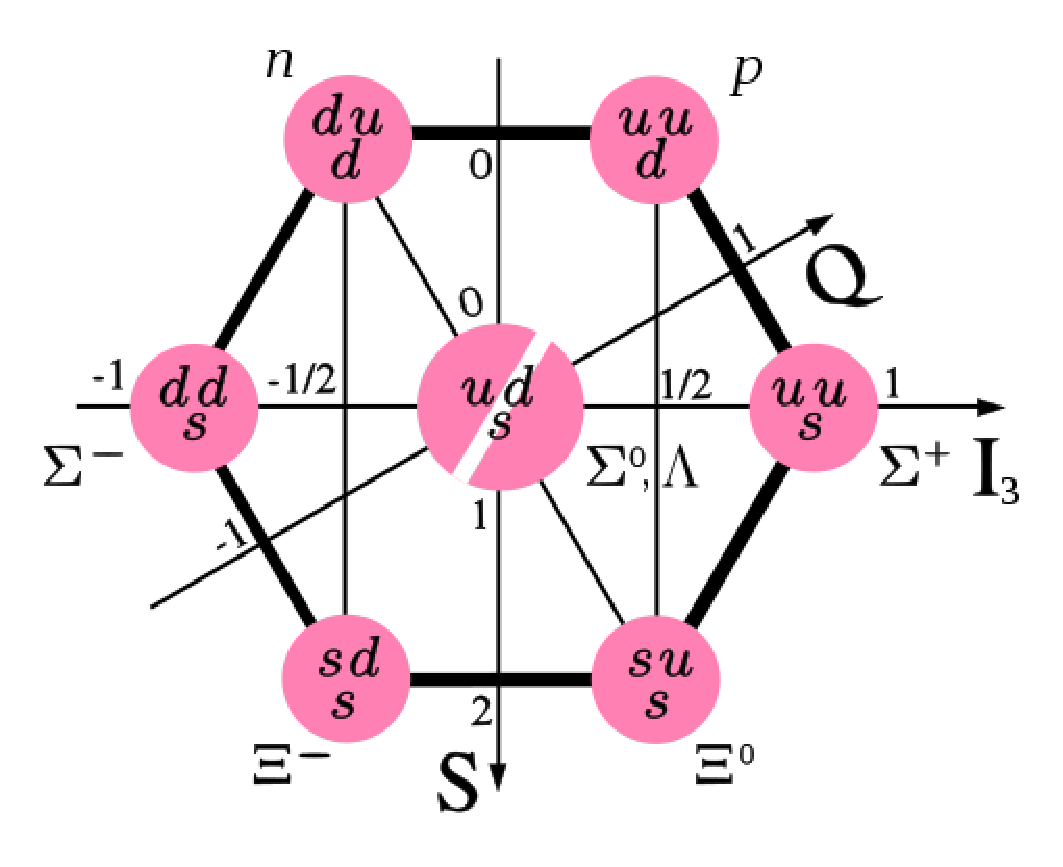
\includegraphics[scale=0.4]{pics/baryon_octet}
\end{center}
\caption{Barionski oktet}
\label{fig:baryon_octet}
\end{figure}

Vidi sliku $\ref{fig:baryon_octet}$ \dots

\section{Struktura grupe SU(3)}

Znamo da grupe SU(N) imaju $N^2-1$ generatora, što znači da ih SU(3) ima osam.
Općeniti element grupe će stoga biti $\exp(i \sum_{A=1}^8 \alpha_A T_{A})$, gdje
su $\alpha_A$ realni parametri, a $T_A$ generatori. Algebra grupe je
\begin{equation}
  [ T_{A}, T_{B} ] = i f_{ABC} T_C \;
\label{eq:SU3}
\end{equation}
gdje su $f_{ABC}$ strukturne konstante grupe. Kao i kod SU(2), ove strukturne
konstante su potpuno antisimetrične u sva tri indeksa (vidi zadatak \thechapter.\ref{zad:fabc}).
Kao i kod SU(2) gdje su generatori u definicionoj (najnižoj netrivijalnoj)
reprezentaciji bili dani $2\times 2$ Paulijevim matricama, tako su generatori
definicione trodimenzionalne reprezentacije grupe SU(3) dani kao
$T_A = \lambda_A/2$, gdje su $\lambda_A$ tzv. Gell-Mannove matrice:

\begin{gather}
\lambda_1 = \begin{pmatrix} 0 & 1 & 0 \\ 1 & 0 & 0 \\ 0 & 0 & 0 \end{pmatrix}\:,\quad
\lambda_2 = \begin{pmatrix} 0 & -i & 0 \\ i & 0 & 0 \\ 0 & 0 & 0 \end{pmatrix}\:,\quad
\lambda_3 = \begin{pmatrix} 1 & 0 & 0 \\ 0 & -1 & 0 \\ 0 & 0 & 0 \end{pmatrix}\:, \nonumber \\[2ex]
\lambda_4 = \begin{pmatrix} 0 & 0 & 1 \\ 0 & 0 & 0 \\ 1 & 0 & 0 \end{pmatrix}\:,\quad
\lambda_5 = \begin{pmatrix} 0 & 0 & -i \\ 0 & 0 & 0 \\ i & 0 & 0 \end{pmatrix}\:,\quad
\lambda_6 = \begin{pmatrix} 0 & 0 & 0 \\ 0 & 0 & 1 \\ 0 & 1 & 0 \end{pmatrix}\:, \\[2ex]
\lambda_7 = \begin{pmatrix} 0 & 0 & 0 \\ 0 & 0 & -i \\ 0 & i & 0 \end{pmatrix}\:,\quad
\lambda_8 = \frac{1}{\sqrt{3}} \begin{pmatrix} 1 & 0 & 0 \\ 0 & 1 & 0 \\ 0 & 0 & -2 \end{pmatrix}
\:.
\nonumber
\end{gather}

Predfaktori su odabrani tako da univerzalno vrijedi relacija normalizacije
\begin{equation}
 \Tr(T_A T_B) = \frac{1}{2} \delta_{AB} \;,
\label{eq:SU3norm}
\end{equation}
koja vrijedi i za grupu SU(2).

Vidljivo je da su prve tri Gell-Mannove matrice zapravo Paulijeve matrice
proširene na tri dimenzije iz čega se vidi da one generiraju SU(2) podgrupu od SU(3).

Strukturne konstante grupe SU(3) su:

\begin{gather}
f_{123} = 1 \, \nonumber \\
f_{147} = -f_{156} = f_{246} = f_{257} = f_{345} = -f_{367} = \frac{1}{2} \, \\
f_{458} = f_{678} = \frac{\sqrt{3}}{2} \;. \nonumber
\end{gather}

Kako je $f_{38A}=0$, $T_3$ i $T_8$ komutiraju što povlači da ih je moguće
istovremeno dijagonalizirati što je i napravljeno gornjim izborom
Gell-Mannovih matrica.
Maksimalan broj takvih generatora naziva se \emph{rang} algebre i oni razapinju
tzv. \emph{Cartanovu podalgebru} date Lieve algebre. 
Algebra su(3) je ranga 2, dok je su(2) ranga 1 (jedino je $\sigma_3$ dijagonalna).

\section{SU(3) tenzori}

Za grupu SU(2) smo identificirali sve njene ireducibilne reprezentacije
razmatrajući isključivo same generatore grupe i njihove komutacijske relacije.
Slična procedure je u načelu moguća i za SU(3), ali mi ćemo se ovdje osloniti
na intuitivniji pristup koji se fokusira na same vektorske prostore na kojima
reprezentacije djeluju. Postupke i rezultate ćemo prikazati na razini
recepta, bez detaljnog dokazivanja.


Pogledajmo prvo analognu proceduru za slučaj grupe SU(2).
Sve ireducibilne reprezentacije te grupe mogu se dobiti
višestrukim direktnim množenjem fundamentalne dvodimenzionalne reprezentacije
(dubleta) sa samom sobom. (Fizikalno govoreći, kombinirajući dovoljan broj
sustava spina $1/2$ možemo dobiti sustav bilo kojeg spina.). Npr. ukoliko
fundamentalni dublet označimo kao
$\psi^a$, $a=1,2$, gdje je 
\begin{displaymath}
 \psi^1 \equiv \ket{\fhalf,\fhalf} \;, \quad \psi^2
\equiv \ket{\fhalf, -\fhalf} \;,
\end{displaymath}
onda direktan produkt tog dubleta sa samim sobom daje četiri stanja:
\begin{displaymath}
 \psi^{11}\equiv \psi^1 \otimes \psi^1 \;, \quad \psi^{12} \;, \quad \psi^{21} \;
 \quad \text{i} \quad \psi^{22} \;.
\end{displaymath}
No, znamo da su ireducibilne reprezentacije od SU(2) zapravo 
\emph{antisimetrični} singlet
\begin{displaymath}
   \psi^{12} - \psi^{21}
\end{displaymath}
i \emph{simetrični} triplet
\begin{displaymath}
 \psi^{11},  \psi^{12} + \psi^{21}, \psi^{22} \;.
\end{displaymath}
Ova potreba da se ireducibilne reprezentacije formiraju 
simetrizacijom i antisimetrizacijom je djelomično rasvijetljena
u odjeljku \ref{sect:sfericniVSkartezijevi} gdje je pokazano 
kako se simetrične i antisimetrične komponente 
tenzora\footnote{U ovom odjeljku riječ tenzor se odnosi na ove
direktne produkte \emph{vektora stanja}, a ne na sferične i kartezijeve
tenzorske \emph{operatore} iz odjeljka \protect\ref{sect:tenzorskioperatori}.
Opisana metoda konstrukcije IRREPsa se po tome i često zove 
``tenzorska metoda''.} ne miješaju pri transformacijama.

Na isti način, direktnim množenjem i (anti)simetriziranjem
fundamentalnih trodimenzionalnih reprezentacija grupe SU(3) moguće
je konstruirati sve njene IRREPse. Kao prvo, potrebno je uočiti da
SU(3) ima \emph{dvije} neekvivalentne 3D reprezentacije,
čiji operatori su povezani kompleksnom konjugacijom: $U(g)$ i
$U(g)^*$. (Za SU(2) grupu su odgovarajuće 2D reprezentacije ekvivalentne
pa je dovoljno raditi samo s jednim fundamentalnim dubletom, vidi
zadatak \thechapter.\ref{zad:su2dublet}.)
Da bismo razlikovali te dvije reprezentacije, odgovarajuće vektore
ćemo označavati s gornjim ili donjim indeksom:
\begin{align}
 3&: \qquad  \psi^a \to \psi^{'a} = \tensor{U}{^a_b} \, \psi^{b} \;, \\
 3^*&: \qquad  \psi_a \to \psi^{'}_a = \tensor{U}{^*_a^b} \, \psi_{b} \;.
\label{eq:su3fundamental}
\end{align}
Reprezentaciju 3 obično zovemo \emph{triplet}, a
reprezentaciju $3^*$ \emph{antitriplet}.
Direktnim množenjem ovih dviju  reprezentacija dobivamo 
tenzore višeg ranga, $\psi^{ab\cdots}_{r\cdots}$, koji
se transformiraju kao:
\begin{equation}
  \psi^{ab\cdots}_{r\cdots} \to 
 \tensor{U}{^{a}_{a'}} \tensor{U}{^{b}_{b'}} \cdots \tensor{U}{^*_r^{r'}} \cdots
  \psi^{a'b'\cdots}_{r'\cdots} \;.
\label{eq:mntensor}
\end{equation}

Promotrimo sada direktni produkt 3 i $3^*$ reprezentacija tj.
tenzor $\psi^a \psi_b$.
Kao prvo, trag tog tenzora je invarijantan i predstavlja tenzor 
ranga 0:
%\begin{displaymath}
%\psi^a \psi_a \to \tensor{U}{^a_b}\tensor{U}{^*_a^c} \psi^b \psi_c
%= \big\{ \tensor{U}{^*_a^c}=\tensor{U}{^\dagger^c_a} \big\}
%= \tensor{(U^\dagger U)}{^c_b} \psi^b \psi_c
%= \tensor{\delta}{^c_b} \psi^b \psi_c = \psi^b \psi_b \.
%\end{displaymath}
To nam sugerira da tenzor $\psi^a \psi_b$ rastavimo 
 dio s tragom nula i sam trag:
\begin{equation}
\psi^a \psi_b = \left(\psi^a \psi_b - \frac{1}{3}
\tensor{\delta}{^a_b}\psi^c \psi_c \right) +
\frac{1}{3} \tensor{\delta}{^a_b} \psi^c \psi_c  \;.
\label{eq:rastav3c3tensor}
\end{equation}
Daljnje rastavljanje odvajanjem simetričnog i antisimetričnog
dijela tenzora nije moguće jer gornji i donji indeks
nisu ekvivalentni. Kako smo ustanovili da je trag ranga 0,
dakle singlet, imamo konačno:
\begin{equation}
  3 \otimes 3^* = 8 \oplus 1 \;.
\label{eq:rastav3c3}
\end{equation}

\subsubsection{Invarijantni SU(3) tenzori}

Kroneckerov simbol $\tensor{\delta}{^a_b}$ je također SU(3) 
tenzor (vidi (\ref{eq:rastav3c3tensor})) i to invarijantan jer:
\begin{equation*}
\tensor{\delta}{^a_b} \to  \tensor{U}{^a_c}
\tensor{U}{^*_b^d} \tensor{\delta}{^c_d} = 
\tensor{U}{^a_c} \tensor{U}{^*_b^c} = \tensor{\delta}{^a_b} \;.
\end{equation*}

Na sličan način se je moguće uvjeriti da su Levi-Civita
tenzori $\epsilon^{abc}$  i $\epsilon_{abc}$ 
također invarijantni, vidi zadatak \thechapter.\ref{zad:epsSU3invariance}. 
Značaj Levi-Civita tenzora je da se pomoću
njih mogu ``spuštati i dizati indeksi'' drugih tenzora.
Npr. promotrimo antisimetričnu komponentu tenzora $\psi^{ab}$,
koju dobijemo kao $\tensor{\psi}{^{[ab]}} \equiv (\psi^{ab}-\psi^{ba})/2$.
Ona očito ima samo tri nezavisne komponente. Množenjem s 
Levi-Civita tenzorom možemo tu činjenicu učiniti eksplicitnom
i pokazati da je $\tensor{\psi}{^{[ab]}}$ ekvivalentan
antitripletu $\psi_a$:
\begin{equation}
  \psi_a = \epsilon_{abc} \tensor{\psi}{^{bc}}
\label{eq:spustanjeindeksa}
\end{equation}
(Objekt $\epsilon_{abc} \tensor{\psi}{^{bc}}$ ima samo jedan slobodan
donji indeks  iz čega se vidi da je ekvivalentan tenzoru $\psi_a$.)

\begin{primjer}[$3\otimes 3$]
Kako triplet i antitriplet nisu ekvivalentni, $3\otimes 3
\neq 3\otimes 3^*$. Kako su u
$3\otimes 3 = \psi^a \psi^b$ oba indeksa istog tipa,
možemo razdvojiti simetrični i antisimetrični dio ovog
tenzora koji su svaki za sebe ireducibilni,
\begin{align}
\psi^a \psi^b &= \fhalf (\psi^a\psi^b + \psi^b \psi^a)
               + \fhalf (\psi^a\psi^b - \psi^b \psi^a) \\
              &\equiv \psi^{(ab)} + \psi^{[ab]}
\end{align}
Prvi, potpuno simetrični član, ima šest nezavisnih komponenata
(broj nezavisnih elemenata simetrične 3$\times$3 matrice) i
predstavlja sekstuplet (6) reprezentaciju.
Nadalje, zahvaljujući svojstvu Levi-Civita tenzora
(usporedi zadatak \ref{ch:lie}.\ref{zad:LeviCivitaProperties}),
$\epsilon^{abc}\epsilon_{cmn} = 
\tensor{\delta}{^a_m}
\tensor{\delta}{^b_n} -
\tensor{\delta}{^a_n}
\tensor{\delta}{^b_m}$, imamo
\begin{equation}
\psi^a\psi^b - \psi^b \psi^a = \epsilon^{abc}\epsilon_{cmn}
\psi^m\psi^n \;.
\end{equation}
$\epsilon^{abc}$ je SU(3) invarijanta, dok je, cf. 
(\ref{eq:spustanjeindeksa}), $\epsilon_{cmn}\psi^{m}\psi^n = \psi_c$
iz čega vidimo da je $\psi^{[ab]}$ ekvivalentan antitripletu
$\psi_c$. 

Podsjetimo se da smo u odjeljku \ref{sect:tenzorskioperatori},
simetrične 6-dim operatore dodatno reducirali na jednodimenzionalni
trag i 5-dim simetrični dio s tragom nula.  Ovdje to ne možemo učiniti
jer na raspolaganju imamo samo 
$\tensor{\delta}{^a_b}$ i $\tensor{\delta}{_a^b}$ kao SU(3) invarijante, 
ali ne i $\delta^{ab}$. (U odjeljku \ref{sect:tenzorskioperatori}
to nije bio problem jer zbog ekvivalentnosti dubleta i antidubleta u
SU(2) ne moramo paziti na razliku između gornjih i donjih indeksa.)
Stoga je $\psi^{(ab)}$ ireducibilni sekstet (6).

Dakle, konačni rezultat je
\begin{equation}
 3 \otimes 3 = 6 \oplus 3^*
\label{eq:33eq63}
\end{equation}
\end{primjer}

\begin{primjer}[$3\otimes 3\otimes 3$]
Koristimo prvo rezultat iz zadnjeg primjera:
\begin{equation}
3\otimes 3\otimes 3 = (3 \otimes 6) \oplus (3 \otimes 3^*) \;.
\end{equation}
Drugi član već znamo iz (\ref{eq:rastav3c3}), a prvi je
umnožak seksteta $\psi^{(ab)}$ i tripleta $\psi^{c}$.
Iz tog umnoška možemo izdvojiti potpuno simetričnu komponentu:
\begin{equation}
\psi^{(ab)}\psi^{c} = \psi^{(abc)} + \text{ostatak} \;. 
\label{eq:6x3}
\end{equation}
Tenzor $\psi^{(abc)}$, tipa $(3,0)$, je totalno simetrični
tenzor ranga 3. Broj njegovih nezavisnih komponenata može
se odrediti npr. izravnim brojanjem. Prvo, postoji
samo jedna nezavisna komponenta sa sva tri različita
indeksa, npr. $\psi^{123}$, i sve ostale su joj jednake:
$\psi^{123} = \psi^{213} = \psi^{312} = \ldots$. Komponenata
s dva ista indeksa i trećim različitim ima šest:
$\psi^{112}, \psi^{113}, \psi^{221}, \psi^{223},
\psi^{331}$ i $\psi^{332}$. Imamo još i tri nezavisne
komponente sa sva tri indeksa ista (na ``hiperdijagonali''
tenzora), $\psi^{111}, \psi^{222}, \psi^{333}$, što sve skupa
čini ukupno 10 komponenata. Dakle, $\psi^{(abc)}$ je
dekuplet (10). Preostali dio u rastavu $3 \otimes 6$ ima
dimenziju $3\times6-10=8$ i odgovara oktetu (8). (Tu
zadnju ekvivalenciju nije lako pokazati ovom tenzorskom
metodom --- pokazat ćemo to u zadatku \thechapter.\ref{zad:3x3x3} 
metodom iz slijedećeg odjeljka.)

Dakle, konačni rezultat je
\begin{equation}
 3 \otimes 3 \otimes 3 = 10 \oplus 8 \oplus 8 \oplus 1
\label{eq:3x3x3}
\end{equation}

Ovaj primjer je od velikog fizikalnog značaja jer odgovara
mogućim kombinacijama triju lakih kvarkova koji čine
fundamentalni SU(3) triplet:
\begin{equation}
 \psi^{1}=u\;, \quad \psi^{2}=d \;, \quad \psi^{3} = s \;,
\end{equation}
Jedan od okteta, prikazan na slici \ref{fig:baryon_octet}, sadrži 
proton i neutron.
\end{primjer}

Tenzorske metode analize SU(3) ireducibilnih reprezentacija, prikazane
u ovom odjeljku, su pogodne jer istovremeno pokazuju strukturu samih
SU(3) objekata što je često od interesa u primjenama, gdje ti objekti
odgovaraju kvantnomehaničkim stanjima. Međutim, kako
dimenzije reprezentacija rastu, i s njima broj indeksa tenzora,
metoda postaje komplicirana. Jednostavnija za primjenu i općenitija
je metoda Youngovih dijagrama, koju predstavljamo u 
slijedećem odjeljku.


\section{SU(N) tenzori i Youngovi dijagrami}

Youngov dijagram je dijagram poput ovog
$$
\ydiagram{5,5,3,1}
$$
gdje je važno svojstvo konveksnosti prema dolje desno tj. da
je lijeva strana poravnata i da se broj polja u retcima
\emph{ne smanjuje} kako idemo odozgo prema dolje.
Dakle, slijedeći dijagrami \emph{nisu} ispravni Youngovi dijagrami
$$
\ydiagram{2+1,3,3} \qquad  \qquad  \ydiagram{3,4,1}
$$
Youngov dijagram s $n$ polja je ekvivalentan SU(N) tenzoru s
$n$ indeksa kojem su prvo indeksi koji odgovaraju pojedinim
retcima dijagrama simetrizirani, a zatim indeksi koji odgovaraju
pojedinim stupcima antisimetrizirani.
\begin{equation}
\ytableaushort{abc, de} \qquad \Longleftrightarrow \qquad
\psi^{[ad][be]c} \;.
\label{eq:tbltensor}
\end{equation}
Uočite da antisimetrizacija po stupcima pokvari simetriju po retcima.
Ukoliko je u ovom primjeru riječ o SU(3) tenzoru, znamo da je par
antisimetriziranih gornjih indeksa ekvivalentan jednom donjem indeksu
nakon spuštanja pomoću Levi-Civita tenzora:
\begin{equation}
SU(3):\quad 
\ytableaushort{abc, de} \qquad \Longleftrightarrow \qquad
\psi^{[ad][be]c} \qquad \Longleftrightarrow \qquad
\psi^{c}_{fg} \;.
\label{eq:tbltensorsu3}
\end{equation}
Na sličan način možemo svaki tenzor (dakle svaku IRREP) prikazati
posebnim Youngovim dijagramom. Npr. u SU(3):
\begin{align}
\ydiagram{1} \qquad\qquad \psi^a \qquad\qquad 3  \\[2ex]
\ydiagram{1,1} \qquad\qquad \psi^{[ab]} \Leftrightarrow \psi_c  \qquad\qquad 3^*  \\[2ex]
\ydiagram{2} \qquad\qquad \psi^{(ab)}  \qquad\qquad 6  \\[2ex]
\ydiagram{1,1,1} \qquad\qquad \psi^{[abc]} \propto \epsilon^{abc} \qquad\qquad 1
\end{align}
U zadnjem redu smo iskoristili činjenicu da je potpuno antisimetrični tenzor s tri
indeksa nužno proporcionalan Levi-Civiti, što znači da je invarijantan i
da ga trebamo tretirati kao singlet tj. jedinični element u algebri
reprezentacija. Ekvivalentno, stupac s N polja
Youngovog dijagrama SU(N) grupe možemo brisati. Dijagram s više od N polja
je naprosto nula jer npr. nije moguće napraviti potpuno antisimetrični tenzor
s četiri indeksa u SU(3) gdje indeksi poprimaju
samo vrijednosti $1$, $2$ i $3$ pa dva od ta četiri indeksa nužno moraju
biti jednaka.

\subsubsection{Dimenzija SU(N) IRREPsa reprezentiranog Youngovim dijagramom}

Youngov dijagram obrojčimo na dva slijedeća načina:

Prvi način: U lijevi gornji kut upišemo $N$ (za SU(N)), i ostatak
reda obrojčimo s sukcesivno rastučim brojevima. Slijedeći red isto,
ali počnemo s $N-1$. I tako dalje.
\begin{displaymath}
\ytableausetup{boxsize=2.5em}
\begin{ytableau} 
\scriptstyle N &\scriptstyle N+1 &\scriptstyle N+2 \\
\scriptstyle N-1 &\scriptstyle N \\
\scriptstyle N-2 \\
\scriptstyle N-3
\end{ytableau}
\end{displaymath}

Drugi način: svako polje dijagrama dobije broj određen ``pravilom kuke''.
Kuka je linija koja od tog polja ide desno u beskonačnost i od tog
istog polja dolje u beskonačnost. Broj polja preko kojih
kuka prolazi upišemo u dato polje. Postupak ponavljamo za sva polja.

%\begin{figure}[ht]
\begin{center}
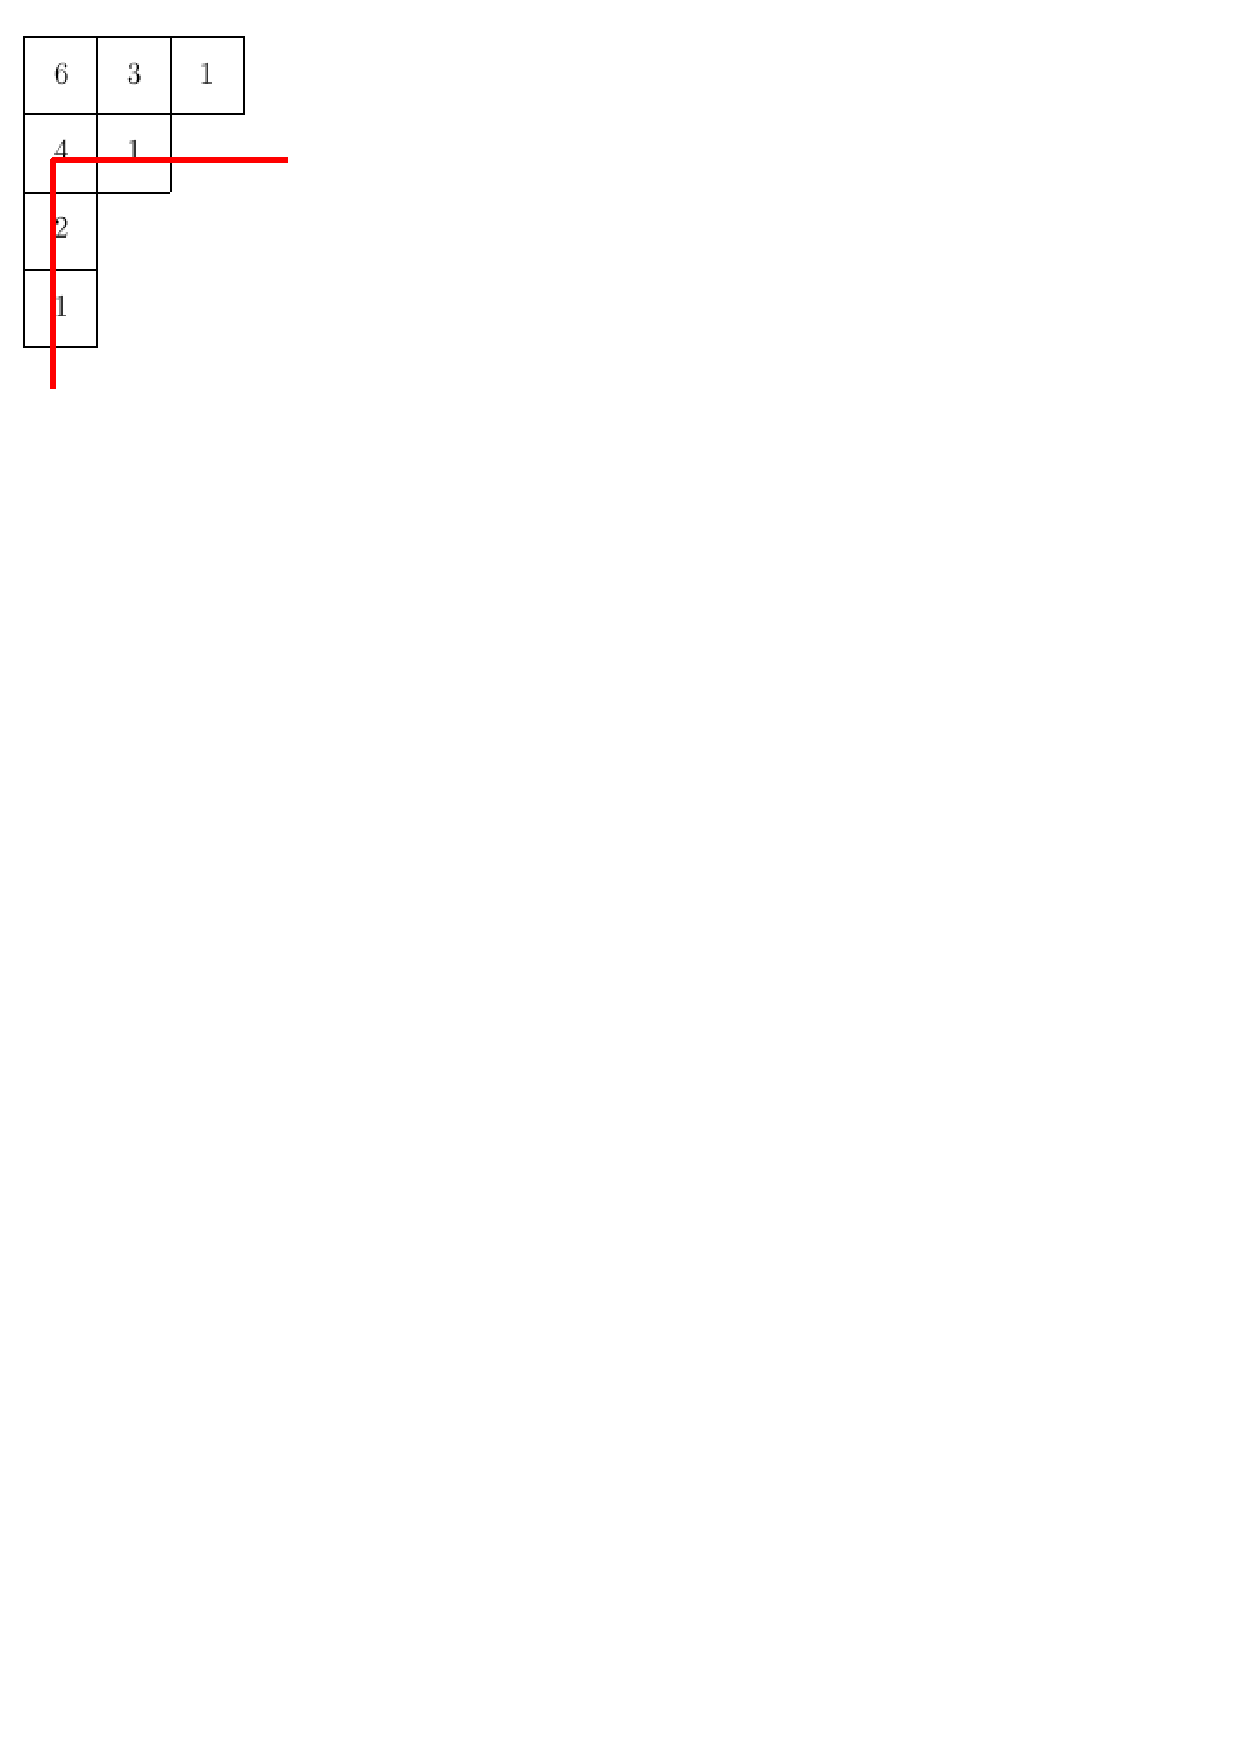
\includegraphics[scale=0.8]{pics/kukat}
\end{center}
%\caption{Barionski oktet}
%\label{fig:baryon_octet}
%\end{figure}
%\begin{displaymath}
%\ytableausetup{boxsize=2.5em}
%\ytableaushort{631, 41, 2, 1}
%\end{displaymath}

Pomnožimo posebno sve brojeve u dijagramu obrojčenom na prvi način i
posebno sve brojeve u dijagramu obrojčenom na drugi način. Dimenzija
IRREPsa je omjer ta dva broja.

Primjeri:

\begin{displaymath}
\ytableausetup{boxsize=normal}
SU(3): \qquad \frac{\ytableaushort{34,2}}{\ytableaushort{31,1}} = \frac{24}{3}= 8
\qquad
\frac{\ytableaushort{3}}{\ytableaushort{1}} = \frac{3}{1}= 3
\qquad
\frac{\ytableaushort{3,2}}{\ytableaushort{2,1}} = \frac{6}{2}= 3^*
\end{displaymath}

U zadnjem od gornja tri primjera smo se oslonili na informacije s
početka ovog odjeljka da bi odredili da je zadnja reprezentacija zapravo
antitriplet.

\begin{displaymath}
SU(3): \qquad \frac{\ytableaushort{34}}{\ytableaushort{21}} = \frac{12}{2}= 6
\qquad
\frac{\ytableaushort{345}}{\ytableaushort{321}} = \frac{60}{6}= 10
\end{displaymath}

\begin{displaymath}
SU(3): \qquad \frac{\ytableaushort{345,234}}{\ytableaushort{432,321}} = 10
 \qquad 
\frac{\ytableaushort{3456,23}}{\ytableaushort{5421,21}} = 27
\end{displaymath}

\begin{displaymath}
SU(5): \qquad \frac{\ytableaushort{56,4}}{\ytableaushort{31,1}} = 40
\end{displaymath}

\subsubsection{Clebsch-Gordanov razvoj za SU(N) IRREPse}

Rastav direktnog produkta dva SU(N) IRREPsa na direktan zbroj
(Clebsch-Gordanov razvoj) izvodi se množenjem odgovarajućih
Youngovih dijagrama, $T_1$ i $T_2$, na slijedeći način. Polja u desnom
dijagramu ozačimo slovima: polja prvog retka
s $a$, polja drugog retka s $b$ i tako dalje:

\begin{displaymath}
\renewcommand{\arraystretch}{2}
\begin{array}{c}
\ydiagram{2,1,1} \\ T_1
\end{array}
 \qquad \otimes \qquad 
\begin{array}{c}
\ytableaushort{aaa,bb,c} \\ T_2
\end{array}
\end{displaymath}

Sada prebacujemo polja s $T_1$ na $T_2$ jedno po jedno, redak
po redak, odozgo prema dolje, na sve moguće načine, tako da
budu zadovoljena slijedeća pravila.
\begin{enumerate}
\item $T_1$ je u svakom trenutku ispravni Youngov dijagram.
\item Polja s istim slovom ne smiju biti u istom stupcu.
 (Posljedica činjenice da su stupci antisimetrizirani.)
\item Za svako polje nastajućeg tenzora je definiran $n_a$
kao broj polja s indeksom $a$ iznad i desno od njega.
Isto tako $n_b$ itd. Mora biti: $n_a \ge n_b \ge n_c$.
\end{enumerate}
Na kraju 
\begin{itemize}
\item Maknemo stupce s $N$ polja. (Jer je totalno
antisimetrični tenzor s $N$ indeksa proporcionalan
s $\epsilon^{a_1 a_2 \cdots a_N}$ i time SU(N)
invarijanta.)
\item Dva dijagrama istog oblika  odgovaraju
posebnim IRREPsima samo ako se razlikuju po razmještaju
slova $a,b,\dots$. U suprotnom jednog maknemo.
\end{itemize}

\begin{primjer}[$8 \otimes 8$ u SU(3)]
\begin{displaymath}
\ydiagram{2,1} \quad\otimes\quad \ytableaushort{aa,b} \quad = 
\end{displaymath}
Jedno {\ytableausetup{smalltableaux}$\ytableaushort{a}$
\ytableausetup{nosmalltableaux}} se može premjestiti na
$T_1$ na tri različita načina
\begin{displaymath}
\left( 
\ytableaushort{\none \none a,\none} * {3, 1}
\quad \oplus \quad
\ytableaushort{\none \none, \none a} * {2, 2}
\quad \oplus \quad
\ytableaushort{\none \none, \none, a} * {2, 1, 1}
\right) 
\quad\otimes\quad \ytableaushort{a,b} \quad = 
\end{displaymath}
Sad premještamo drugo {\ytableausetup{smalltableaux}$\ytableaushort{a}$
\ytableausetup{nosmalltableaux}}:
\begin{align*}
\left( 
\ytableaushort{\none \none a a,\none} * {4, 1}
\quad\oplus\quad 
\ytableaushort{\none \none a, \none a} * {3, 2}
\quad\oplus\quad 
\ytableaushort{\none \none a, \none, a} * {3, 1, 1}
\right)& 
\quad\otimes\quad \ytableaushort{b}  \\
\quad\oplus\quad\left( 
\ytableaushort{\none \none a,\none a} * {3, 2}
\quad\oplus\quad 
\ytableaushort{\none \none, \none a, a} * {2, 2, 1}
\right)& 
\quad\otimes\quad \ytableaushort{b}  \\
\quad\oplus\quad\left( 
\ytableaushort{\none \none a,\none, a} * {3, 1, 1}
\quad\oplus\quad 
\ytableaushort{\none \none, \none a, a} * {2, 2, 1}
\right)& 
\quad\otimes\quad \ytableaushort{b} \quad=
\end{align*}
Tu imamo tri dijagrama u duplikatu pa po jedan maknemo:
\begin{displaymath}
\left( 
\ytableaushort{\none \none a a,\none} * {4, 1}
\quad\oplus\quad 
\ytableaushort{\none \none a, \none a} * {3, 2}
\quad\oplus\quad 
\ytableaushort{\none \none a, \none, a} * {3, 1, 1}
\quad\oplus\quad 
\ytableaushort{\none \none, \none a, a} * {2, 2, 1}
\right) 
\quad\otimes\quad \ytableaushort{b} \quad=
\end{displaymath}
\begin{multline*}
\ytableaushort{\none \none a a,\none b} * {4, 2}
\quad\oplus\quad 
\ytableaushort{\none \none a a,\none, b} * {4, 1, 1}
\quad\oplus\quad 
\ytableaushort{\none \none a, \none a b} * {3, 3} \\
\quad\oplus\quad 
\ytableaushort{\none \none a, \none a, b} * {3, 2, 1}
\quad\oplus\quad 
\ytableaushort{\none \none a, \none b, a} * {3, 2, 1}
\quad\oplus\quad 
\ytableaushort{\none \none , \none a, a b} * {2, 2, 2}
\end{multline*}
Primijetite da ovdje nismo kreirali dijagrame koji
narušavaju gornja pravila:
\begin{displaymath}
\ytableaushort{\none \none a a b, \none} * {5, 1}
\qquad \text{i} \qquad
\ytableaushort{\none \none a, \none, a, b} * {3, 1,1, 1}
\end{displaymath}
Sada maknemo sve stupce s tri polja (SU(3) invarijante)
i dobijemo konačno:
\begin{equation*}
\ytableaushort{\none \none a a,\none b} * {4, 2}
\quad\oplus\quad 
\ytableaushort{\none a a} * {3}
\quad\oplus\quad 
\ytableaushort{\none \none a, \none a b} * {3, 3}
\quad\oplus\quad 
\ytableaushort{\none a, a} * {2, 1}
\quad\oplus\quad 
\ytableaushort{\none a,  b} * {2, 1}
\quad\oplus\quad 
1
\end{equation*}
Dimenzije IRREPsa za sve ove dijagrame smo već odredili pa
očitavamo konačni rezultat
\begin{equation}
8 \otimes 8 = 27 \oplus 10 \oplus 10 \oplus 8 \oplus 8 \oplus 1
\label{eq:8x8}
\end{equation}
(Zgodno je uočiti da je postupak jednostavniji ako pri množenju
kao desni uzmemo Youngov dijagram s manje polja.)

\end{primjer}

\subsection*{Zadaci}

\begin{enumerate}[label=\arabic{chapter}.\arabic*.]

\item Ako pretpostavimo očuvanje izospina, koja su moguća izospinska
stanja (ukupni izospin i treća komponenta ukupnog izospina) pri
raspršenju protona na

 \begin{description} \item[a)] $\pi^+$
                     \item[b)] $\pi^0$
                     \item[c)] $\pi^-$. \end{description}


\item \label{zad:fabc}
Pokažite da su, zahvaljujući komutacijskim relacijama i relaciji (\ref{eq:SU3norm}),
strukturne konstante $f_{ABC}$, grupe SO(3) potpuno antisimetrične u
svim indeksima.

\item \label{zad:su2dublet}
Pokažite da je za SU(2)  $2^* = 2$ tj. da su fundamentalni dublet i
antidublet ekvivalentni, tako da pokažete da je operator $C$
\begin{displaymath}
  C = U(R(\hat{y},\theta=\pi)) = \exp\left(-\frac{i}{\hbar} J_2 \pi\right) \;
\end{displaymath}
operator koji povezuje 2 i $2^*$:
\begin{align*}
C \sigma_i C^{-1}& = - \sigma_{i}^* \\
C U(g) C^{-1}& = U(g)^*
\end{align*}

\item \label{zad:epsSU3invariance}
Pokažite da su Levi-Civita tenzori $\epsilon^{abc}$ i $\epsilon_{abc}$
invarijatni na SU(3) transformacije. Naputak: promotrite djelovanje
infinitezimalnih transformacija $U=1+i\alpha_A T_A$.

\item \label{zad:3x3x3}
Izračunajte Clebsch-Gordanov razvoj u SU(3) grupi za
\begin{itemize}
\item $3^* \otimes 3$
\item $3 \otimes 3$
\item $3 \otimes 3 \otimes 3$
\end{itemize}

\item Izračunajte Clebsch-Gordanov razvoj u SU(6) grupi za
\begin{itemize}
\item $6 \otimes 6^*$
\item $6 \otimes 6 \otimes 6$
\end{itemize}

\end{enumerate}

\fancypagestyle{plain}{%
    \fancyhf{}
    \fancyhead[RO,LE]{\bfseries \thepage}
    \fancyhead[CO]{\rightmark}
    \fancyhead[CE]{\leftmark}
    \renewcommand{\headrulewidth}{0.4pt}}

\chapter{Lorentzova i Poincar\'{e}ova simetrija}

Iz dosadašnjih poglavlja trebalo bi biti jasno da je moć
neke simetrije to veća što je odgovarajuća grupa veća, što
će za kontinuirane (Liejeve) grupe obično značiti da je broj generatora
grupe veći. Stanja fizikalnih sustava i jednadžbe ili lagranžijani
koji tim sustavima upravljaju
će u tom slučaju biti više ograničeni zahtjevima kovarijantnosti
na transformacije simetrije i predviđanja koja su posljedica
primjene teorije grupa će biti netrivijalnija i općenitija.
Dodatnu moć simetrije dobivaju od netrivijalnih komutacijskih
relacija između generatora simetrija.
Tako već i razmjerno jednostavana simetrija na rotacije ima izuzetno
netrivijalne posljedice, kako smo vidjeli u \ref{ch:rotacije}. poglavlju.
Prirodno je onda postaviti pitanje koja je maksimalna
simetrija koju teorije prirode moraju poštivati. Osim rotacija,
maksimalna grupa simetrija svakako treba sadržavati i translacije
u prostoru i vremenu, koje smo sreli u odjeljcima
\ref{sec:prostornetranslacije} i \ref{sec:vremensketranslacije}.
Već i kombiniranje ovih transformacija u istu grupu simetrija
nije trivijalno jer translacije i rotacije ne komutiraju. To je
vidljivo i iz običnih razmatranja geometrije u prostoru, a i iz 
neiščezavajućih komutacijskih relacija odgovarajućih
kvantnomehaničkih operatora impulsa $\vec{p}$ i momenta
impulsa $\vec{J}$.

\begin{equation}
    [J_{i}, p_{j}] = \rmi \hbar \epsilon_{ijk} p_{k} \;.
    \label{eq:jpkomutacijske}
\end{equation}

Pokazuje se da osim upravo navedenih transformacija, maksimalna
grupa simetrija koja upravlja najuniverzalnijim poznatim zakonima
prirode, onima kvantne teorije polja, od kontinuiranih prostornovremenskih
transformacija sadrži još samo Lorentzove transformacije među inercijalnim sustavima,
poznate kao Lorentzovi \emph{potisci} (engl. \emph{boost}).
Ta maksimalna grupa se obično naziva Poincar\'{e}ova\footnote{Priroda poštuje
    i općenitije trasformacije prostorvremena poznate kao difeomorfizmi. 
    Odgovarajuće simetrije poštuje klasična Einsteinova teorija gravitacije, ali još
    ih nismo uspjeli ugraditi u univerzalne kvantne teorije ostalih sila i
    tim simetrijama se ne bavimo u ovoj knjizi. Ne bavimo se ni \emph{konformnom}
    grupom simetrija koja Poincar\'{e}ovim transformacijama dodaje i
    dilatacije $x^{\mu}\to\lambda x^{\mu}$ što je simetrija koja prema
    trenutnim spoznajama nije egzaktna simetrija prirode,
    ali je svejedno od velikog teorijskog interesa.}.
Prije nego se pozabavimo Poincar\'{e}ovom grupom i njenim reprezentacijama,
pogledat ćemo prvo u sljedeća dva odjeljka grupno-teorijska svojstva samih
Lorentzovih potisaka koji, kako ćemo vidjeti, ne tvore grupu samostalno
nego tek u kombinaciji s rotacijama.


\section{Lorentzova grupa}
\label{sec:lorentz}

Einsteinova specijalna teorija relativnosti počiva na tzv.
principu relativnosti. Prema njemu, postoji skup ekvivalentnih koordinatnih
sustava (zvanih \emph{inercijalni sustavi})
u međusobnom jednolikom pravocrtnom gibanju, a u kojima fizikalni zakoni i pojave
izgledaju isto. Promatrač ne može eksperimentalno detektirati da 
se giba, ako se giba jednoliko. Mirovanje nije apsolutno,
čega su na ovaj ili onaj način bili svjesni već Kopernik, Galilei i Newton, ali je
tek Einstein uočio druge radikalne posljedice ovog načela, poput toga
da ni simultanost događaja nije apsolutna.
Princip relativnosti je princip simetrije na troparametarski skup transformacija
koje preslikavaju inercijalne sustave jedan u drugi.
Da bismo vidjeli o kojoj se grupi simetrija radi (i da li se uopće radi o grupi),
moramo ustanoviti kako se kombiniraju transformacije među inercijalnim sustavima.

Kako je poznato, iz principa relativnosti slijedi da
transformacije iz sustava $S=\{t,x,y,x\}$ u sustav $S'=\{t',x',y',x'\}$, 
tzv. \emph{Lorentzovi potisci}, imaju oblik\footnote{U
standardnoj literaturi se pri izvodu Lorentzovih potisaka osim principa
relativnosti obično koristi i postulat o konstantnosti brzine svjetlosti
u svim sustavima.  No, ovaj drugi postulat je zapravo suvišan, vidi
Mermin, Am. J. Phys. \textbf{52}(2) (1984) 119 ili J. D. Jackson,
\emph{Classical Electrodynamics}, 3rd ed.(!), zadaci 11.1 i 11.2.}
\begin{align}
t' &= \gamma \big(t-\frac{\beta}{c}z\big) \,, \\
x' &= x \,, \\
y' &= y \,,  \\
z' &= \gamma \big(z-\beta ct \big) \,,
\end{align}
gdje je $c$ brzina svjetlosti i
gdje je radi jednostavnosti uzeto da se je brzina $\vec{v}$ relativnog gibanja
dvaju sustava duž $z$-osi, $\vec{v}=v\hat{\vec{z}}$, te su uvedene standardne pokrate
\begin{displaymath}
 \beta \equiv \frac{v}{c} \,, \qquad \qquad \gamma\equiv\frac{1}{
\sqrt{1-\beta^2}} \,.
\end{displaymath}
Ove transformacije djeluju na četverodimenzionalnom vektorskom prostoru koji
se zove \emph{prostor Minkowskog} i kojeg sačinjavaju tzv.
\emph{Lorentzovi vektori}
$x^\mu$,  $\mu=0,1,2,3$, čije su komponente  $x^0=ct, x^1=x, x^2=y$ i $x^3=z$.
U prostoru Minkowskog je vektorski produkt dvaju vektora definiran kao
\begin{equation}
    (x, y) \equiv x \cdot y \equiv x^0 y^0 - x^1 y^1 - x^2 y^2 - x^3 y^3 \,,
    \label{eq:produktminkowskog}
\end{equation}
pa je  pogodno definirati i tzv. \emph{kovarijantne}
komponente istog vektora s donjim indeksima
$x_0=ct, x_1=-x, x_2=-y, x_3=-z$, tako da je skalarni produkt jednostavno
\begin{equation}
x \cdot y = x^{\mu} y_{\mu} \;.
\end{equation}
\emph{Metrički tenzor}
\begin{equation}
g = 
\begin{pmatrix}
1 & 0 & 0 & 0 \\
0 &-1 & 0 & 0 \\
0 & 0 &-1 & 0 \\
0 & 0 & 0 &-1
\end{pmatrix} \,,
    \label{eq:metrickitenzor}
\end{equation}
omogućuje pretvorbu donjih kovarijantnih u gornje (\emph{kontravarijantne})
indekse tako da je
\begin{align}
x^\mu &= (ct, \vec{x}) \\
x_\mu &= (ct,-\vec{x}) = g_{\mu\nu} x^\nu
\end{align}
te skalarni produkt zapisujemo i kao\footnote{Specifično 
razlikovanje "gornjih" i "donjih" indeksa vektora u
specijalnoj teoriji relativnosti služi samo jednostavnom zapisu
skalarnog produkta u prostoru Minkowskog.
U \emph{općoj} teoriji relativnosti to razlikovanje dviju vrsta
koordinata prelazi u razlikovanje dviju vrsta vektora 
(\emph{kovarijantni} i \emph{kontravarijantni} vektori), odnosno,
još preciznije, jezikom diferencijalne geometrije razlikujemo 
\emph{vektore} i \emph{1-forme}, ali ovdje nam te finese ne igraju
nikakvu ulogu.}
\begin{equation}
     x \cdot y = g_{\mu\nu} x^{\mu}x^{\nu} \;.
\end{equation}
Izraženo preko ovih Lorentzovih vektora (zvanih i \emph{četverovektori}),
Lorentzovi potisci poprimaju oblik 
\begin{align}
x'^{0} &= \gamma (x^0 - \beta x^3 ) \\
x'^{1} &= x^1 \,, \\
x'^{2} &= x^2 \,, \\
x'^{3} &= \gamma (x^3 -\beta x^0 ) \;,
\end{align}
ili u kompaktnom obliku
\begin{equation}
    x'^{\mu} = \tensor{\Lambda}{^{\mu}_{\nu}} x^\nu \;, \qquad
\tensor{\Lambda}{^{\mu}_{\nu}} =
\begin{pmatrix}
\gamma & 0 & 0 & -\beta\gamma \\
0 & 1 & 0 & 0 \\
0 & 0 & 1 & 0 \\
-\beta\gamma & 0 & 0 & \gamma
\end{pmatrix} \;.
\label{eq:deflambda}
\end{equation}
Očekujemo da će se jednadžbe
relativističke fizike izgrađivati od vektora koji se transformiraju
kao i $x^{\mu}$, te odgovarajućih
skalara i tenzora, koji se transformiraju množenjem s brojem $\Lambda$ matrica
koji odgovara njihovom rangu, baš kao što se u nerelativističkoj fizici jednadžbe
izgrađuju od tenzora s dobrim transformacijskim svojstvima pri prostornim rotacijama,
definiranim u (\ref{eq:tenzor}).

Matrice $\Lambda$ ovise o parametrima Lorentzovog
potiska kojeg je prirodno parametrizirati vektorom brzine $\vec{v}$ pojedinog
inercijalnog sustava u odnosu na neki referentni sustav.
 Vidimo da Lorentzovi potisci $\Lambda(\vec{v})$ čine 3-parametarski
skup. Da li je on grupa? Kako ćemo eksplicitno pokazati u slijedećem
odjeljku odgovor je \emph{ne}. Kompozicija dva Lorentzova potiska, ako
isti nisu kolinearni, nije
samo Lorentzov potisak već kompozicija
Lorentzovog potiska i prostorne rotacije
\begin{equation}
 \Lambda(\vec{v}_2) \circ \Lambda(\vec{v}_1)
  = R(\vec{v}_2,\vec{v}_1) \circ \Lambda(\vec{v}_2,\vec{v}_1) \;,
\end{equation}
čija je  poznata posljedica pojava tzv. \emph{Thomasove precesije}. 
Tek skup svih Lorentzovih potisaka
i prostornih rotacija čini grupu, za čiju je identifikaciju najlakše
osloniti se na definiciju grupe kao skupa transformacija koji
ostavljaju skalarni produkt invarijantan, kako smo radili
u odjeljku \ref{sec:primjeriLie}, gdje smo definirali
pseudo-ortogonalnu grupu \O{1, 3} upravo kao grupu transformacija
koja ostavlja invarijantnim kvadratnu formu koja
odgovara skalarnom produktu (\ref{eq:produktminkowskog}).
Stoga se \O{1,3} često naziva \emph{opća Lorentzova grupa}.
Grupa prostornih rotacija \SO{3}
je podgrupa ove grupe koja čuva produkt (\ref{eq:produktminkowskog}) tako
da čuva njen prostorni dio, a ne dira vremenski dio. Skup Lorentzovih
potisaka $\{\Lambda(\vec{v})\}$ je podskup ove grupe, ali ne i podgrupa.

Za transformirani 4-vektor $x' = \Lambda x$ vrijedi
\begin{align}
 {x'}^2 &= g_{\mu\nu} {x'}^\mu {x'}^\nu \\
        &= ({x^0}', {x^1}', {x^2}', {x^3}')
\begin{pmatrix}
1 & 0 & 0 & 0 \\
0 &-1 & 0 & 0 \\
0 & 0 &-1 & 0 \\
0 & 0 & 0 &-1
\end{pmatrix}
\begin{pmatrix}
{x^0}' \\ {x^1}' \\ {x^2}' \\ {x^3}'
\end{pmatrix} \\
  &= {x'}^{\top} g x' = x^\top \Lambda^\top g \Lambda x \\
  &= x^2 = x^\top g x
\end{align}
pa usporedbom dobivamo definiciju opće Lorentzove grupe
\O{1, 3}
kao grupe svih matrica $\Lambda$ sa svojstvom
\begin{equation}
   \Lambda^\top g \Lambda = g
\label{deflambda}
\end{equation}
što je definicija koju smo upoznali već u (\ref{eq:MgM}).
Uzimanjem determinante ove matrične jednadžbe, uz svojstva
da je za svaku matricu $\det A^\top = \det A$ te da je za
metrički tenzor $\det g = -1$ dobijemo 
\begin{equation}
   (\det \Lambda)^2 = 1 \,,
\end{equation}
iz čega slijedi da je
\begin{equation}
   \det\Lambda = \pm 1 \;.
\label{detL}
\end{equation}
Ova situacija je analogna situaciji u grupi \O{3} čiji elementi
također imaju determinantu $\pm 1$ pa (vidi argumentaciju na
stranici \pageref{pag:povezanostO3}) elementi koji imaju
determinantu $+1$ i tako čine podgrupu \SO{1, 3} nisu topološki
u grupnoj mnogostrukosti povezani sa elementima koji imaju
determinantu $-1$. Za razliku od \O{3}, koja ima točno te
dvije komponente povezanosti (vidi (\ref{eq:so3Pso3})), 
vidjet ćemo da ih \O{1, 3} ima četiri.
Naime, raspišimo matričnu jednadžbu (\ref{eq:deflambda})  po komponentama
\begin{equation}
    \underbrace{\tensor{(\Lambda^\top)}{_{\mu}^{\nu}}}_{\tensor{\Lambda}{^{\nu}_{\mu}}}
    g_{\nu\rho}\tensor{\Lambda}{^{\rho}_{\sigma}} = g_{\mu\sigma}
\end{equation}
i pogledajmo komponentu $\mu=\sigma=0$. Kako je $g_{00}=1$ imamo
\begin{align}
    1 &= g_{\nu\rho} \tensor{\Lambda}{^{\nu}_{0}} \tensor{\Lambda}{^{\rho}_{0}}  \\
      &= (\tensor{\Lambda}{^{0}_{0}})^2 - \sum_{i=1}^{3}(\tensor{\Lambda}{^{i}_{0}})^2 \;.
\end{align}
Slijedi da je 
\begin{equation}
    (\tensor{\Lambda}{^{0}_{0}})^2 = 1 + \sum_{i=1}^{3}(\tensor{\Lambda}{^{i}_{0}})^2 \,,
\end{equation}
odnosno da je $(\tensor{\Lambda}{^{0}_{0}})^2 \geq 1$ što daje dvije mogućnosti:
\begin{equation}
    \tensor{\Lambda}{^{0}_{0}}\geq 1  \qquad\text{ili}\qquad \tensor{\Lambda}{^{0}_{0}}\leq -1 \;.
\end{equation}
Zajedno s dvije mogućnosti za $\det \Lambda$ imamo dakle četiri mogućnosti koje vode
na četiri odvojene komponente povezanosti od O(1,3)
\begin{center}
\renewcommand{\arraystretch}{1.3}
\begin{tabular}{ccc}
\hline
$\det\Lambda$ & $\tensor{\Lambda}{^{0}_{0}}$ & oznaka   \\ \hline
1         &  $\geq 1$   & \SOsup{+}{1,3} \\
 -1           &  $\geq 1$   & $P\,\SOsup{+}{1,3}$ \\
 1           &  $\leq -1$   & $\SOsup{-}{1,3} = PT\,\SOsup{+}{1,3}$ \\
 -1           &  $\leq -1$   & $T\,\SOsup{+}{1,3}$ \\ \hline
\end{tabular}
\renewcommand{\arraystretch}{1.0}
\end{center}
gdje smo izdvojili specijalne elemente grupe \O{1, 3} 
prostornu inverziju (\emph{paritet}) $P$
i vremensku inverziju $T$, definirane kao
\begin{align}
    P& =g :  (t\to t, \vec{x}\to -\vec{x}) \,, \label{eq:paritet} \\
    T& =-g :  (t\to -t, \vec{x}\to \vec{x})  \;.
\end{align}
Komponenta povezanosti jedinice
\SOsup{+}{1,3} je od najvećeg interesa i
nekad se naziva \emph{prava ortokrona Lorentzova grupa}, a neki autori koriste i
samo za nju termin Lorentzova grupa, što ćemo i mi dalje običavati. Iz tablice vidimo da
se svi elementi pune Lorentzove grupe \O{1,3} mogu prikazati kao produkt jedne od transformacija
iz skupa $\{1, P, T, PT\}$ i elemenata \SOsup{+}{1,3}.


\section{Generatori i reprezentacije Lorentzove grupe}
\label{sec:genLor}

Kao i kod rotacija, objekte koji se pojavljuju u našim teorijama treba klasificirati prema
njihovim transformacijskim svojstvima pri Lorentzovim transformacijama
tj. prema pripadnosti reprezentacijama Lorentzove
grupe. Kao i kod rotacija, poželjno je usredotočiti se na Lievu algebru
grupe koju čine generatori $L$:
\begin{equation}
    \Lambda \in \SOsup{+}{1,3} \,, \qquad \Lambda = e^L \,.
\end{equation}
Iz definicionog svojstva (\ref{deflambda}) dobijemo $L^\top g = -g L$,
što uz činjenicu da je $g^\top = g$ daje $(gL)^\top = -gL$ odnosno
vidimo da je $gL$ antisimetrična matrica. To znači da ako $L$
parametriziramo na slijedeći način
\begin{align}
 gL &= 
\begin{pmatrix}
1 & 0 & 0 & 0 \\
0 &-1 & 0 & 0 \\
0 & 0 &-1 & 0 \\
0 & 0 & 0 &-1
\end{pmatrix}
\begin{pmatrix}
L_{00} & L_{01} & L_{02} & L_{03}\\
L_{10} &\hdotsfor{3} \\
\hdotsfor{4} \\
\hdotsfor{3} & L_{33}
\end{pmatrix} \\[1ex]
&= 
\begin{pmatrix}
L_{00} & L_{01} & L_{02} & L_{03}\\
-L_{10} & -L_{11} & -L_{12} &\hdotsfor{1} \\
-L_{20} & -L_{21} & \hdotsfor{2} \\
\hdotsfor{3} & -L_{33}
\end{pmatrix} \,,
\end{align}
svojstvo antisimetrije $gL$ traži
\begin{align}
L_{0i} &= L_{i0} \,, \\
L_{ij} &= - L_{ji} \;.
\end{align}
tj.
\begin{equation}
 L = \begin{pmatrix}
0 & L_{01} & L_{02} & L_{03}\\
L_{01} & 0 & L_{12} & L_{13}\\
L_{02} & -L_{12} & 0& L_{23} \\
L_{03} & -L_{13} &-L_{23} & 0
\end{pmatrix} \;,
\end{equation}
gdje tri parametra $L_{01}$, $L_{02}$ i $L_{03}$ opisuju Lorentzove
potiske, a tri parametra $L_{12}$, $L_{13}$ i $L_{23}$ prostorne rotacije.
Umjesto ovih šest parametara pogodno je koristiti parametre
$\theta_i$ i $\zeta_i$,  definirane na slijedeći način:
\begin{equation}
 L = -i (\theta_i J_i + \zeta_i K_i)  \qquad i=1,2,3  \;,
\label{eq:LJK}
\end{equation}
gdje su $J_i$ već dobro poznati generatori rotacija, samo prošireni
na četverodimenzionalni prostor Minkowskog
\begin{equation}
 J_1 =
\begin{pmatrix}
0 & 0 & 0 & 0 \\
0 & 0 & 0 & 0 \\
0 & 0 & 0 & -i \\
0 & 0 & i & 0
\end{pmatrix} \quad
 J_2 =
\begin{pmatrix}
0 & 0 & 0 & 0 \\
0 & 0 & 0 & i \\
0 & 0 & 0 & 0 \\
0 & -i & 0 & 0
\end{pmatrix} \quad
J_3 =
\begin{pmatrix}
0 & 0 & 0 & 0 \\
0 & 0 & -i & 0 \\
0 & i & 0 & 0 \\
0 & 0 & 0 & 0
\label{eq:defJi}
\end{pmatrix} \,,
\end{equation}
dok su $K_i$ generatori Lorentzovih potisaka
\begin{equation}
K_1 =
\begin{pmatrix}
0 & -i & 0 & 0 \\
-i & 0 & 0 & 0 \\
0 & 0 & 0 & 0 \\
0 & 0 & 0 & 0
\end{pmatrix} \;
K_2=
\begin{pmatrix}
0 & 0 & -i & 0 \\
0 & 0 & 0 & 0 \\
-i & 0 & 0 & 0 \\
0 & 0 & 0 & 0
\end{pmatrix} \;
K_3 =
\begin{pmatrix}
0 & 0 & 0 & -i \\
0 & 0 & 0 & 0 \\
0 & 0 & 0 & 0 \\
-i & 0 & 0 & 0
\end{pmatrix} \,.
\label{eq:defKi}
\end{equation}

Treba primijetiti kako operatori $K_i$ nisu hermitski tako da odgovarajuće
transformacije $\exp(-i\zeta_i K_i)$ neće biti unitarne. To je posljedica
nekompaktnosti Lorentzove grupe --- parametri potiska poprimaju
vrijednosti iz nekompaktnog intervala $[0,c)$.
Kao posljedica toga integrali po grupnom prostoru ne konvergiraju i ta se beskonačnost
za unitarne reprezentacije mora odražavati u beskonačnosti vektorskih prostora
na kojima one djeluju. Konačnodimenzionalne reprezentacije nekompaktnih grupa
su obavezno neunitarne, gdje jedino trivijalna jednodimenzionalna reprezentacija
čini iznimku. Kao primjer toga, matrice $\tensor{\Lambda}{^\mu_\nu}$
definicione četverodimenzionalne reprezentacija Lorenztove grupe u (\ref{eq:deflambda}) 
su očito neunitarne. Stoga se stanja kvantnih sustava za koja je 
unitarnost obavezna prema Wignerovom teoremu (vidi dodatak \ref{sec:qm}) ne mogu transformirati
prema konačnodimenzionalnim reprezentacijama. U sljedećem odjeljku ćemo
vidjeti kako se ona transformiraju prema beskonačnodimenzionalnim
reprezentacijama Poincar\'{e}ove grupe (koja sadrži Lorenztovu),
dok su konačnodimenzionalne neunitarne reprezentacije koje diskutiramo
u ostatku ovog odjeljka relevantne za objekte za koje unitarnost
nije nužna poput četverovektora položaja ili impulsa te, važno, klasičnih
i kvantnih polja.


Pogledajmo prvo komutacijske relacije Lorentzove Lieve algebre \soAlg{1,3}. Eksplicitnim
množenjem vidimo da vrijedi
\begin{align}
[J_i, J_j] &= i\epsilon_{ijk} J_k  \,, \label{eq:LK1}\\
[K_i, K_j] &= -i\epsilon_{ijk} J_k \,, \label{eq:LK2} \\
[J_i, K_j] &= i\epsilon_{ijk} K_k \;. \label{eq:LK3}
\end{align}
Prva relacija je dobro poznata algebra \soAlg{3}=\suAlg{2} grupe prostornih rotacija
koja je dakle podgrupa Lorentzove grupe.
Druga relacija govori da podskup Lorentzovih potisaka nije zatvoren
i ne čini grupu, kako smo najavili u prošlom odjeljku. Treća
relacija govori da tri generatora potisaka $K_i$ čine kartezijev vektor obzirom
na rotacije, vidi (\ref{eq:jvkomutacija}).
Ove tri komutacijske relacije su vrlo slične onima iz odjeljka \ref{sec:so4} gdje smo 
rastavili grupu SO(4) na direktan produkt SU(2)$\otimes$SU(2) identificirajući
kombinacije generatora koji zatvaraju dvije neovisne podgrupe.
Slično ćemo postupiti i ovdje te definirati
\begin{equation}
  \vec{J}^{(\pm)} \equiv \fhalf \big(\vec{J}\pm i \vec{K} \big) \;,
  \label{eq:defJpm}
\end{equation}
odnosno $\vec{J}=\vec{J}^{(+)}+\vec{J}^{(-)}$, $\vec{K} = -i
(\vec{J}^{(+)}-\vec{J}^{(-)})$. Primijetite dodatni ``$i$'' obzirom
na situaciju u odjeljku \ref{sec:so4} koji je potreban zbog
minus predznaka u (\ref{eq:LK2}).
Uz ovakve definicije vidimo da su (\ref{eq:LK1})--(\ref{eq:LK3}) ekvivalentne
dvjema odvojenim \suAlg{2} algebrama
\begin{align}
[J_{i}^{(+)}, J_{j}^{(+)}] &= i \epsilon_{ijk} J_{k}^{(+)} \,, \\
[J_{i}^{(-)}, J_{j}^{(-)}] &= i \epsilon_{ijk} J_{k}^{(-)} \,, \\
[J_{i}^{(+)}, J_{j}^{(-)}] &= 0  \;.
\end{align}
Ovo ipak ne znači  da O(1,3) ima istu algebru kao i SU(2)$\otimes$SU(2),
jer gore u (\ref{eq:defJpm})  nismo radili \emph{realne} linearne kombinacije generatora,
a podsjećamo da su sve Liejeve algebre u ovoj knjizi nad $\mathbb{R}$.
Svejedno ispostavlja se\footnote{nakon vrlo netrivijalnog postupka \emph{kompleksifikacije}
Lieve algebre} da za klasifikaciju ireducibilnih reprezentacija Lorentzove
grupe možemo kao i u odjeljku \ref{sec:so4} koristiti parove
\begin{equation}
(j^{(+)}, j^{(-)})  \qquad j^{(+)}, j^{(-)} = 0, \fhalf, 1, \dotsc .
\end{equation}
Tako imamo trivijalnu 1D (0,0) reprezentaciju i objekte koji se
transformiraju prema njoj zovemo Lorentzovi skalari. Slijedeće
dvije su 2D tzv. \emph{Weylove} reprezentacije ($\fhalf$, 0) i
(0, $\fhalf$) prema kojima bi se transformirala bezmasena
fermionska polja, kad bi takva postojala, što u ovom trenutku nije poznato.
Obični četverovektori poput $x^\mu$ pripadaju ireducibilnoj
4D reprezentaciji $(\fhalf, \fhalf)$. Uočite da ukoliko napravimo
restrikciju Lorentzove simetrije \SOsup{+}{1,3} na samo rotacijsku \SO{3},
ireducibilna reprezentacija $(\fhalf, \fhalf)$ postaje reducibilna,
pa kako je $\vec{J}=\vec{J}^{(+)}+\vec{J}^{(-)}$ standardni 
Clebsch-Gordanov razvoj ("zbrajanje" momenata impulsa) nam kaže da
je 
\begin{equation}
(j^{(+)}=\fhalf, j^{(-)}=\fhalf)_{\SOsup{+}{1,3}} \quad = \quad(j=1)_{\SO{3}} \oplus (j=0)_{\SO{3}} \,,
\end{equation} 
gdje naravno trodimenzionalni $j=1$ potprostor odgovara prostornim vektorima,
a jednodimenzionalni $j=0$ potprostor vremenskoj komponenti koja je invarijantna
na rotacije.

Za Diracovu jednadžbu koja opisuje \emph{masivna} fermionska polja poput elektronskog, 
poznato je da udružuje lijeve
i desne komponente pa je \SOsup{+}{1,3} pravu
ortokronu Lorentzovu grupu potrebno proširiti operacijom pariteta $P$ i onda
identificirati ireducibilne reprezentacije obzirom
na ovu veću grupu. Operator pariteta (\ref{eq:paritet}) 
matrično izgleda kao
\begin{equation}
 P = P^{-1} =
\begin{pmatrix}
1 & 0 & 0 & 0 \\
0 & -1 & 0 & 0 \\
0 & 0 & -1 & 0 \\
0 & 0 & 0 & -1
\end{pmatrix} \;,
\end{equation}
i eksplicitnim djelovanjem na (\ref{eq:defJi}) i (\ref{eq:defKi}) 
je vidljivo da se pri prostornoj inverziji generatori rotacije
transformiraju kao aksijalni vektori (vidi dodatak \ref{sec:aksijalni}),
\begin{equation}
    P^{-1} \vec{J} P = \vec{J} \;,
\end{equation}
a generatori Lorentzovih potisaka kao pravi polarni vektori,
\begin{equation}
    P^{-1} \vec{K} P = - \vec{K} \;.
\end{equation}
Slijedi da je 
\begin{equation}
    P^{-1} \vec{J}^{(\pm)} P = \vec{J}^{(\mp)} \;.
\end{equation}
Posljedično, proširivanjem \SOsup{+}{1,3} grupe paritetom, reprezentacije
(0, $\fhalf$) i ($\fhalf$,0) više nisu ireducibilne svaka zasebno,
već ireducibilna postaje 4D reprezentacija $(\fhalf, 0) \oplus (0, \fhalf)$, poznata
kao Diracova reprezentacija.


Slično, tenzor elektromagnetskog polja $F^{\mu\nu}$ pripada
6-dimenzionalnoj reducibilnoj reprezentaciji (1,0)$\oplus$(0,1).


Kao što smo u \ref{ch:rotacije}. poglavlju i od samih operatora tražili
dobro definirana tenzorska svojstva obzirom na rotacije
(npr. tri generatora $J_i$ čine vektor obzirom na rotacije), tako
je i u kontekstu Lorentzove simetrije moguće generatore i
same elemente grupe definirati na način koji manifestno pokazuje
kovarijantnost obzirom na Lorentzove transformacije.
Dakle, želimo relacije poput (\ref{eq:LJK}) i (\ref{eq:LK1})--(\ref{eq:LK3}) 
zapisati u 4-komponentnoj notaciji, putem Lorentzovih tenzora.
To postižemo definiranjem antisimetričnih generatora 
grupe \SOsup{+}{1,3} $J^{\mu\nu}$ kao
\begin{align}
J^{mn}& = \epsilon^{mni} J^i \,, \label{eq:defJmn}\\
J^{i0}& = K^i \;.
\label{eq:defJi0}
\end{align}
(Podsjetimo se da grčki indeksi idu $\alpha,\beta = 0,1,2,3$, a 
latinski $i,m = 1,2,3$.)  
Sada je element grupe \SOsup{+}{1,3} dan kao
\begin{equation}
 \Lambda = \exp\left(-\frac{i}{2} \omega_{\rho\sigma} J^{\rho\sigma}\right) \,,
\label{eq:4DLorentz}
\end{equation}
a komutacijske relacije (\ref{eq:LK1})--(\ref{eq:LK3}) se ujedinjuju u
\begin{equation}
i [ J^{\mu\nu}, J^{\rho\sigma}] = g^{\mu\rho} J^{\nu\sigma}
- g^{\nu\rho} J^{\mu\sigma} + g^{\sigma\mu} J^{\rho\nu}
- g^{\sigma\nu} J^{\rho\mu} \;.
\label{eq:4DLorKom}
\end{equation}
Također, matrični elementi generatora Lorentzove grupe u
4D definicionoj ($\fhalf$, $\fhalf$) reprezentaciji dani su kao
\begin{equation}
\tensor{(J^{\mu\nu})}{^\alpha_\beta} = i \big(
g^{\mu\alpha}\tensor{\delta}{^\nu_\beta} - \tensor{\delta}{^\mu_\beta}
g^{\nu\alpha} \big) \;.
\label{eq:4DJmn}
\end{equation}
S druge strane matrični elementi generatora Lorentzove grupe u
4D Diracovoj reprezentaciji
$(\fhalf, 0) \oplus (0, \fhalf)$
dani su kao
\begin{equation}
 J^{\mu\nu} = \frac{i}{4} [\gamma^\mu, \gamma^\nu] \;,
\label{eq:DiracJ}
\end{equation}
gdje su $\gamma^\mu$ tzv. Diracove gama matrice definirane
antikomutacijskim relacijama
\begin{equation}
 \gamma^\mu\gamma^\nu + \gamma^\nu \gamma^\mu
\equiv \{\gamma^\mu, \gamma^\nu\} = 2 g^{\mu\nu} \,.
\label{eq:DiracGamma}
\end{equation}
Jedan mogući izbor za ove matrice je
\begin{equation}
\gamma^0 = \left(\begin{array}{rr} \Eins & 0 \\
                        0 & -\Eins \end{array}\right)
\;, \quad
\gamma^i = \left(\begin{array}{rr} 0 & \sigma^i \\
                        -\sigma^i & 0 \end{array}\right) \;,
\end{equation}
gdje su $\sigma^i$ Paulijeve matrice (\ref{eq:PaulijeveMatrice}).

\section{Poincar\'{e}ova grupa}


Poincar\'{e}ova (poznata i kao nehomogena Lorentzova) grupa je
proširenje Lorentzove grupe translacijama u prostoru
i vremenu. Element $(\Lambda, a)$ te grupe djeluje na vektore u prostorvremenu
Minkowskog kao
\begin{equation}
  x^\mu \longrightarrow \tensor{\Lambda}{^\mu_\nu} x^\nu + a^\mu \,,
\label{eq:defPoin}
\end{equation}
gdje je $\tensor{\Lambda}{^\mu_\nu}$ matrica Lorentzove transformacije,
dok su $a^\mu \in \mathbb{R}^{1,3}$ četiri parametra translacija u prostor-vremenu.
Kompozicija elemenata Poincar\'{e}ove grupe, za koju se iz (\ref{eq:defPoin}) 
lako vidi da je oblika
\begin{equation}
    (\Lambda, a) \circ (\bar{\Lambda}, \bar{a})
    = (\Lambda \bar{\Lambda}, \Lambda\bar{a} + a) \;,
\end{equation}
ne zadovoljava definiciju \ref{def:direktniproduktgrupa} direktnog produkta
grupa. To je posljedica činjenice da za razliku od grupe translacija,
Lorentzova grupa nije normalna podgrupa Poincar\'{e}ove grupe.
U takvom slučaju govorimo o \emph{semi-direktnom} produktu grupa
i pišemo da je Poincar\'{e}ova grupa $\mathbb{R}^{1,3} \rtimes \O{1,3}$,
te je označavamo i kao \IO{1,3} ("I" dolazi od engl. \emph{inhomogenous}.
U literaturi se Poinca).

Riječ je očito o deset-parametarskoj grupi gdje povrh generatora
Lorentzove grupe ($J^i$ i $K^i$) imamo i impuls $P^i$ kao
generator translacija u prostoru i Hamiltonijan $H$ kao
generator translacija u vremenu.
Algebra ove grupe je algebra Lorentzove grupe \SO{1,3} (\ref{eq:4DLorKom}) 
i dodatno
\begin{align}
[H, H]& = [H, P^i] = [P^i, P^j] = 0 \label{eq:Poi1} \\
[H, J_i]& = 0  \label{eq:Poi2}\\
[K^i, H]& = i P^i  \label{eq:PoiPuzzle} \\
[J^i, P^j]& = i \epsilon^{ijk} P^k \\
[K^i, P^j]& = i H \delta^{ij} \;,
\label{eq:PoinKom}
\end{align}
što je moguće ujedinjeno napisati u 4-dim notaciji kao
\begin{equation}
i [P^\mu, J^{\rho\sigma}] = g^{\mu\sigma}P^\rho - g^{\mu\rho}P^{\sigma} \;.
\label{eq:4DPoinKom}
\end{equation}
Npr.
\begin{displaymath}
[H, K^i] = [P^0, J^{i0}] = -i(g^{0 0}P^i - g^{0i}P^0) =  -i P^i \;.
\end{displaymath}
Relacije  (\ref{eq:Poi1}) i (\ref{eq:Poi2}) govore da su impuls i
moment impulsa očuvani pri translacijama u vremenu. Zanimljivo je da relacija
(\ref{eq:PoiPuzzle}) govori kako generatori Lorentzovih potisaka
$K^i$ ne komutiraju s Hamiltonijanom što sugerira da ne odgovaraju
očuvanim veličinama. To može biti zbunjujuće jer Noetherin teorem
nam govori kako bi simetrija obzirom na 10-parametarsku Poincar\'{e}ovu grupu
trebala rezultirati s deset očuvanih veličina, a ovako ih imamo samo
7 --- energiju, tri komponente impulsa i tri komponente momenta impulsa.
Razrješenje je u tome da Noetherini očuvani naboji
(pokušajte ih eksplicitno odrediti) koji
odgovaraju Lorentzovim potiscima jesu formalno očuvani (vremenska
derivacija iščezava), ali eksplicitno ovise o vremenskoj 
koordinati\footnote{Slično kao što $J_z = x P_y - y P_z$ 
eksplicitno ovisi o prostornim $x$ i $y$ koordinatama.}
pa nisu od praktične koristi. 


U sljedećem odjeljku ćemo se baviti konstrukcijom unitarnih ireducibilnih
reprezentacija Poincar\'{e}ove grupe koje djeluju na kvantnomehanička stanja.
U tom kontekstu će biti relevantno svojstvo Poincar\'{e}ove grupe da
dopušta i projektivne reprezentacije, vidi odjeljak \ref{sec:projektivnerep},
jer njena komponenta povezanosti
jedinice nije jednostavno povezana. To znači da je kompozicija
transformacija definirana do na fazu.
To je isključivo posljedica
činjenice da je njena podgrupa Lorentzova grupa \SOsup{+}{1,3},
dvostruko povezana. Situacija je potpuno analogna situaciji iz
odjeljka \ref{sec:projektivnerep}, gdje je grupa rotacija
\SO{3} dopuštala projektivne reprezentacije\footnote{Dvostruku
    povezanost Lorentzova grupe direktno nasljeđuje
od njene podgrupe --- grupe rotacija.}. Tamo smo identificirali
jednostavno povezanu grupu pokrivanja \SU{2} koja ima istu algebru
kao i \SO{3}, no čije su sve reprezentacije obične, ne-projektivne.
Za Lorentzovu grupu također postoji grupa pokrivanja. Riječ je
o grupi $\SL{2, \mathbb{C}}$ svih regularnih kompleksnih
$2\times 2$ matrica, koja dva puta pokriva Lorentzovu grupu,
što za posljedicu ima da je i ovdje kompozicija transformacija
na kvantnim stanjima "dvo-vrijedna" i može uključivati dodatni
minus.
U skladu s komentarima na kraju odjeljka \ref{sec:projektivnerep} 
mogli bismo reći da je "istinska" Poincar\'{e}ova grupa
$\mathbb{R}^{1,3} \rtimes \SL{2, \mathbb{C}}$. No mi ćemo
se svejedno držati standardne Poincar\'{e}ove grupe, s
komponentnom povezanosti jedinice $\mathbb{R}^{1,3} \rtimes \SOsup{+}{1,3}$
jer nam je djelovanje elemenata te grupe na prostoru Minkowskog dobro poznato.
S druge strane, pojednostavit ćemo analizu razmatrajući
samo prave reprezentacije grupe, znajući da postoji mogućnost i
projektivnih, što će se na kraju svesti samo na to spinovi mogu
biti i polucjelobrojni, što nije nikakva novost.

\section{Unitarne reprezentacije Poincar\'{e}ove grupe}

Želja nam je klasificirati i opisati unitarne ireducibilne reprezentacije
$U(\Lambda, a)$
Poincar\'{e}ove grupe na Hilbertovom prostoru jednočestičnih stanja 
$\mathcal{H}$. Vektori koji razapinju potprostore od $\mathcal{H}$ koji
pripadaju tim reprezentacijama su labelirani svojstvenim vrijednostima
maksimalnog skupa međusobno komutirajućih generatora grupe
(kako je za grupu rotacija bio samo $J_3$). Poincar\'{e}ova grupa
nije ni kompaktna ni polujednostavna i na nju se ne može primijeniti
metoda slična onoj koju smo koristili za grupu rotacija  gdje smo
identificirali stanje s maksimalnom vrijednošću $J_3$ i onda razapeli
cijeli prostor djelovanjem $J_\pm$.
Za Poincar\'{e}ovu grupu je E. Wigner 1939. godine razvio posebnu
metodu --- tzv. metodu \emph{induciranih reprezentacija} koju ćemo
sada izložiti.

Promatrajući komutacijske relacije Poincar\'{e}ove grupe 
(\ref{eq:LK1})--(\ref{eq:LK3}) i (\ref{eq:Poi1})--(\ref{eq:PoinKom})
prirodno je za označavanje stanja koristiti četveroimpuls $p^{\mu}$,
obzirom da pripadajuća četiri operatora $P^{\mu}$ međusobno komutiraju.
Komponenta $p^0$ je redundantna pa ćemo stanja označavati samo s $\vec{p}$
\begin{equation}
    P^{\mu} \ket{\vec{p}, \sigma} = p^{\mu} \ket{\vec{p}, \sigma} \,,
    \label{eq:defpsigma}
\end{equation}
gdje $\sigma$ označava sve ostale labele potrebne za potpunu specifikaciju
stanja unutar dane ireducibilne reprezentacije, a koje tek treba odrediti\footnote{Dakle,
    $\sigma$ obrojčava ostale dimenzije
vektorskog prostora, ortogonalne na kontinuum dimenzija koje obrojčava $\vec{p}$.}.
Sva stanja $\ket{\vec{p}, \sigma}$ s istim $\vec{p}$, a različitim $\sigma$
razapinju potprostor $\mathcal{H}_{p} \subset \mathcal{H}$ kojeg nazivamo
\emph{mali Hilbertov prostor}. Zahvaljujući (\ref{eq:defpsigma}) djelovanje
čistih translacija je jednostavno, podsjetimo se odjeljka \ref{sec:qmtrans} 
\begin{equation}
    U(1, a) \ket{\vec{p}, \sigma} = e^{\rmi p\cdot a}  \ket{\vec{p}, \sigma}\;.
    \label{eq:PoiTrans}
\end{equation}
Pozabavimo se sada djelovanjem Lorentzovih transformacija $U(\Lambda)\equiv U(\Lambda, 0)$.


Skup vektora $\{ \tensor{\Lambda}{^\mu_\nu}p^{\nu} \: | \: \Lambda \in \SOsup{+}{1,3}\}$
koje dobijemo djelovanjem svih Lorentzovih transformacija na neki
vektor $p$, nazivamo \emph{orbita} tog vektora. Oblik orbite ovisi o karakteristikama
vektora i mogućnosti su prikazane na slici \ref{fig:orbite} i bit će diskutirane kasnije.
Izaberimo neki konkretni element orbite $p^{*}$ kojeg ćemo zvati
\emph{reprezentant} orbite i označiti zvjezdicom (nema veze s kompleksnom konjugacijom).
Konstruirajmo sada skup transformacija 
$\{L(p) \td p \in \mathrm{orbita}(p^*) \} \subset \SOsup{+}{1,3}$ koje
na \emph{jedinstven} način transformiraju $p^{*\mu}$ u svaki vektor njegove orbite
\begin{equation}
p^{\mu} = \tensor{L(p)}{^\mu_\nu} p^{*\nu}\,.
\end{equation}
Označavat ćemo skraćeno $L_{p} \equiv L(p)$.
Elementi $U(L)$ iz unitarne reprezentacije Poincare\'{o}ve grupe
preslikavaju vektore iz $\mathcal{H}_{p^*}$ u $\mathcal{H}_{p}$
i kako je inverz $U(L_{p})^{-1} = U(L_{p}^{-1})$ definiran jer
su $U$ elementi reprezentacije grupe, preslikavanje je injekcija i
svi mali Hilbertovi prostori $\mathcal{H}_{p}$ na orbiti su 
izomorfni. Tako izbor reprezentanta $p^*$ ne smanjuje općenitost
i možemo izabrati bilo koji pogodni reprezentant orbite za daljnju
analizu. Nadalje, kad jednom definiramo bazu  $\mathcal{H}_{p^*}$
(obrojčenu vrijednostima labele $\sigma$), baze ostalih $\mathcal{H}_{p}$
\emph{definiramo} preslikavanjem
\begin{equation}
\ket{\vec{p}, \sigma} \equiv U(L_{p}) \ket{\vec{p}^*, \sigma} \quad \forall \sigma \,.
    \label{eq:defbazaHp}
\end{equation}
Treba uočiti da će konkretne baze ovisiti o skupu $\{L_{p}\}$, a
sastav tog skupa ovisi ne samo o izboru reprezentanta $p^*$ nego i
o izboru elemenata $L_p$ koji na jedinstven način transformiraju
$p^*$ u $p$. Orbitu sačinjavaju vektori različitih iznosa i smjerova
troimpulsa $\vec{p}$,
pa će $L_p$ tipično biti kombinacija potiska i rotacije, ali postoji
sloboda hoćemo li prvo zarotirati $\vec{p}^*$ u smjer $\vec{\hat{p}}$ pa 
napraviti odgovarajući potisak ili obrnuto ili pak neka kompliciranija kombinacija.

Za općenitu Lorentzovu transformaciju $\Lambda \in \SOsup{+}{1,3}$,
između dva proizvoljna vektora $p$ i $\Lambda p$ na orbiti očekujemo 
da odgovarajući operator $U(\Lambda)$ miješa vektore baze
odgovarajućih malih Hilbertovih prostora $\mathcal{H}_{p}$
i $\mathcal{H}_{\Lambda p}$ tj. da je
\begin{equation}
    U(\Lambda) \ket{\vec{p}, \sigma} = \sum_{\sigma'=1}^{\mathrm{dim}(\mathcal{H}_{\Lambda p})}
    C_{\sigma \sigma'} \ket{\Lambda\vec{p}, \sigma'} \,.
\end{equation}
Objekti $C_{\sigma \sigma'}$ (matrice ako je $\mathrm{dim}(\mathcal{H}_{p}) =
\mathrm{dim}(\mathcal{H}_{\Lambda p})$ konačno)
nakon transformacije u blok-dijagonalnu
formu (ako je potrebno) definiraju tražene unitarne ireducibilne reprezentacije
Lorentzove grupe. Ti objekti na kompleksan način ovise o $\Lambda$ i
$p$ eksplicitno te o $L_{p}$ i $p^*$ implicitno,
no sad ćemo vidjeti da su ipak razmjerno jednostavni.

Ograničimo se privremeno na $m > 0$ masivnu situaciju i promotrimo
kao reprezentanta $p^{*\mu} = (m, 0, 0, 0)$.
Pripadajući mali Hilbertov prostor $\mathcal{H}_{p^*}$ je razapet
vektorima $\ket{\vec{p}^{*}, \sigma}$. Djelovanje $U(\Lambda)$ na
proizvoljno stanje na orbiti je
\begin{align}
    U(\Lambda)\ket{\vec{p}, \sigma} &=  U(\Lambda) U(L_p) \ket{\vec{p}^{*}, \sigma} \\
     &= U(\Lambda L_p) \ket{\vec{p}^{*}, \sigma} \\
     &= U(L_{\Lambda p}) U(L_{\Lambda p}^{-1}) \: U(\Lambda L_p) \ket{\vec{p}^{*}, \sigma} \\
     &= U(L_{\Lambda p})\, U(L_{\Lambda p}^{-1} \Lambda L_p) \ket{\vec{p}^{*}, \sigma}
     \label{eq:defRWone}
.\end{align}
gdje smo u prvom redu iskoristili (\ref{eq:defbazaHp}) i gdje smo
obilato koristili svojstvo da je $U(\Lambda)$ reprezentacija\footnote{I gdje
smo po potrebi radili u "istinskoj" Lorentzovoj grupi \SL{2, \mathbb{C}}
umjesto u \SOsup{+}{1,3} da izbjegnemo faze projektivnih reprezentacija,
vidi diskusiju na kraju prošlog odjeljka.}.
Sada treba uočiti da je Lorentzova transformacija koja
u (\ref{eq:defRWone}) djeluje na $\ket{\vec{p}^{*}, \sigma}$ redom
\begin{description}
    \item[1.] transformacija iz sustava mirovanja ($p^*$) u sustav impulsa $p$,
    \item[2.] transformacija u sustav impulsa $\Lambda p$, te
    \item[3.] inverzna transformacija koja nas vraća u sustav mirovanja.
\end{description}
Dakle ukupna Lorentzova transformacija je obična rotacija!
Tu rotaciju
\begin{equation}
    R_{\scriptscriptstyle \mathrm{W}} \equiv L_{\Lambda p}^{-1} \Lambda L_p \,,
    \label{eq:defRW}
\end{equation}
nazivamo \emph{Wignerova rotacija} i nije ju općenito lako eksplicitno
odrediti, no nama je ovdje bitno samo to da je to obična prostorna rotacija
jer djelovanje rotacija na kvantna stanja dobro
znamo. Ono je dano Wignerovim $D$-matricama,
vidi (\ref{eq:WignerD}), pa je odgovarajuća transformacija u $\mathcal{H}_{p^*}$
\begin{equation}
    U(R_{\scriptscriptstyle\rm W}) \ket{\vec{p}^{*}, \sigma} = 
      \sum_{\sigma'=-j}^{j} D^{(j)}_{\sigma'\sigma}(R_{\scriptscriptstyle\rm W})
      \ket{\vec{p}^{*}, \sigma'} \;,
\end{equation}
i vidimo da $\sigma$ nije ništa drugo nego projekcija spina, često
označavana s $m$ ("magnetski" kvantni broj).
Uvrštavanjem u (\ref{eq:defRWone}) dobivamo reprezentaciju Lorentzove
grupe
\begin{equation}
    U(\Lambda) \ket{\vec{p}, \sigma} = 
     \sum_{\sigma'=-j}^{j} D^{(j)}_{\sigma'\sigma}(R_{\scriptscriptstyle\rm W})
     \ket{\Lambda\vec{p}, \sigma'} \;,
\end{equation}
te na kraju i reprezentaciju Poincar\'{e}ove grupe
\begin{equation}
    U(\Lambda, a) \ket{\vec{p}, \sigma} =  e^{\rmi p \cdot a}
     \sum_{\sigma'=-j}^{j} D^{(j)}_{\sigma'\sigma}(R_{\scriptscriptstyle\rm W})
     \ket{\Lambda\vec{p}, \sigma'} \;.
\end{equation}
Centralni je rezultat ovog razmatranja da je, pored mase $m$, standardni spin $j$
jedino drugo svojstvo sustava potrebno za specifikaciju njegovog ponašanja
pri Poincar\'{e}ovim transformacijama.
Masa je svojstvena vrijednost Casimirovog operatora $P^2$, a spin
je svojstvena vrijednost Casimirovog operatora $\vec{J}^2$, koji se
može pogodno generalizirati na kovarijantni operator $W^2$ gdje je
$W^{\mu}$ \emph{operator Paulija i Ljubanskog}
\begin{equation}
    W_{\mu} \equiv - \frac{1}{2} \epsilon_{\mu \nu \rho \sigma}
    J^{\nu \rho} P^{\sigma} \,,
    \label{eq:defPLj}
\end{equation}
gdje je $J^{\nu \rho}$ definiran u (\ref{eq:defJmn})--(\ref{eq:defJi0}).
Čitatelj će se lako uvjeriti da u sustavu mirovanja vrijedi
\begin{equation}
    W^2 = - m^2 \vec{J}^2 = -m^2 j (j+1) \;.
\end{equation}
Par $(m, j)$ potpuno specificira ponašanje sustava pri kompletnom skupu
prostornovremenskih simetrija danih Poincar\'{e}ovom grupom, i često se
govori da je \emph{definicija} "čestice" to da je to sustav koji predstavlja
ireducibilnu reprezentaciju Poincar\'{e}ove grupe ili, alternativno,
da je to sustav definirane mase i spina.
Treba reći da se ovdje ne ograničavamo samo na tzv. elementarne čestice.
I ne-elementarni sustavi, ako ih promatramo u situacijama koje ne razlučuju
njihovu unutarnju građu (npr. proton na energijama na kojima se ne pobuđuju
kvarkovi ili vodikov atom u osnovnom stanju na energijama manjim od 1 eV),
predstavljaju \emph{jednočestična stanja} i ireducibilne reprezentacije
Poincar\'{e}ove grupe.

Spomenimo još da se gore diskutirana sloboda u izboru baza malih Hilbertovih
prostora na orbiti u praksi koristi tako da se, umjesto standardne \emph{spinske}
baze gdje je $\sigma$ svojstveno stanje $J_z$,
koristi \emph{helicitetna} baza gdje je $\sigma$ svojstveno stanje operatora
heliciteta $\vec{J}\cdot\vec{\hat{p}}$, tj. operatora momenta impulsa projeciranog na smjer
impulsa čestice. To ima nekoliko prednosti
\begin{itemize}
    \item Helicitet $\vec{J}\cdot\vec{\hat{p}}$ komutira s impulsom $\vec{P}$ 
        (vidi zadatak \ref{zad:help}) pa je onda stanje $\ket{\vec{p}, \sigma}$
        specificirano pomoću svojstvenih vrijednosti komutirajućih operatora koje
        su istovremeno mjerljive.

   \item U ultrarelativističkom limesu elektromagnetske i jake nuklearne sile
       čuvaju vrijednost heliciteta.

   \item U često korištenom sustavu dvije čestice u kojem njihov ukupni troimpuls
       iščezava, njihov orbitalni moment impulsa je okomit na smjer njihovog
       relativnog gibanja. Tada je ukupni spin duž tog smjera (što je važna očuvana veličina)
       dan jednostavnim zbrajanjem heliciteta bez potrebe dodavanja doprinosa
       orbitalnog momenta impulsa kojeg često ne znamo.
\end{itemize}

Ovo smo razmatranje proveli specijalizirano za sustav s $m > 0$.
Pogledajmo sada općenitu situaciju. U gornjem izvodu ključno je bilo
identificirati grupu simetrija koja ostavlja invarijantnim reprezentirajući
vektor $p^*$. Ta se grupa naziva \emph{mala grupa} ili \emph{stabilizator}
i u gornjem slučaju to je bila grupa rotacija \SO{3}.
Pokazali smo da se puna reprezentacija $U(\Lambda, a)$ inducira iz te
male grupe pa je to bio primjer metode induciranih reprezentacija.
Metoda općenito uključuje identificiranje klasa elemenata vektorskog prostora
(ovdje $p \in \mathbb{R}^{1,3}$) koji su kao skupovi invarijantni na djelovanje
pune grupe (ovdje orbite Poincar\'{e}ove grupe),
identificiranje pogodnih reprezentanata tih klasa $p^*$ i
određivanje njihovih malih grupa. Sve kategorije orbita prikazane su
na slici \ref{fig:orbite}
\begin{figure}[htpb]
    \centering
    \documentclass[border=3mm]{standalone}

\usepackage{tikz}
\usepackage{amsbsy}

\begin{document}
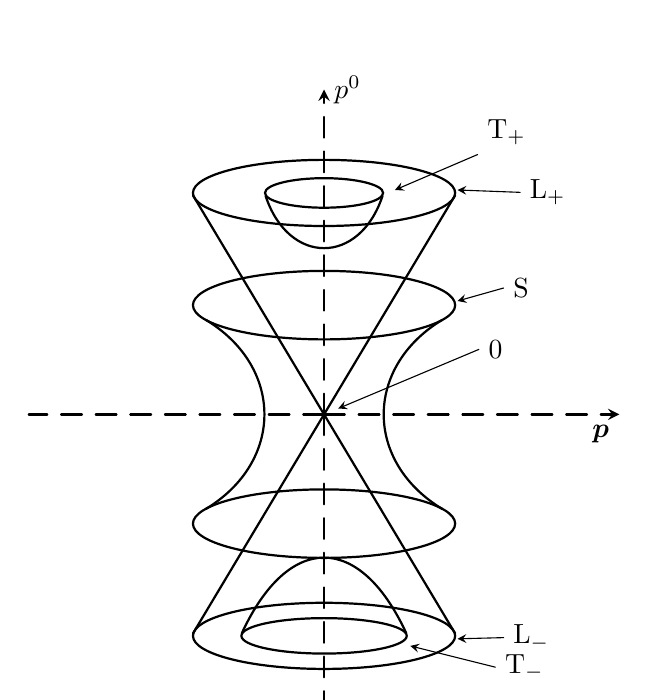
\begin{tikzpicture}[line cap=round,scale=0.75]
\draw[dash pattern=on 7.5pt off 5pt,thick] (0,0) -- (-5,0); 
\draw[dash pattern=on 7.5pt off 5pt,thick,-stealth] (0,0) -- (5,0) node[below left] {$\boldsymbol{p}$};
\draw[dash pattern=on 7.5pt off 5pt,thick] (0,0) -- (0,-5);
\draw[dash pattern=on 7.5pt off 5pt,thick,-stealth] (0,0) -- (0,5.5) node[right] {$p^0$};
\draw[thick]	  (-2.22,3.71) -- (2.22,-3.71);
\draw[thick]	  (2.22,3.71) -- (-2.22,-3.71);
\draw[thick]  (0,3.75) ellipse (2.22 and 0.56);
\draw[thick] (-0.99,3.7) .. controls (-0.6,2.52) and (0.6,2.52) .. (0.99,3.7);
\draw[thick]  (0,3.75) ellipse (1 and 0.25);
\draw[thick]  (0,1.85) ellipse (2.22 and 0.58);
\draw[thick]  (0,-1.85) ellipse (2.22 and 0.58);
\draw[thick] (-1.39,-3.7) .. controls (-0.6,-2) and (0.6,-2) .. (1.39,-3.7);
\draw[thick]  (0,-3.75) ellipse (1.4 and 0.3);
\draw[thick]  (0,-3.75) ellipse (2.22 and 0.56);
\draw[thick] (-2,1.6) .. controls (-0.68,0.8) and (-0.68,-0.8) .. (-2,-1.6);
\draw[thick] (2,1.6) .. controls (0.68,0.8) and (0.68,-0.8) .. (2,-1.6);
\draw[stealth-] (1.2,3.8) -- (2.6,4.4) node[above right] {$\mathrm{T}_+$};
\draw[stealth-] (2.26,3.8) -- (3.32,3.76) node[right] {$\mathrm{L}_+$};
\draw[stealth-] (2.26,1.92) -- (3.04,2.14) node[right] {$\mathrm{S}$};
\draw[stealth-] (0.24,0.1) -- (2.62,1.1) node[right] {$0$};
\draw[stealth-] (2.26,-3.8) -- (3.04,-3.78) node[right] {$\mathrm{L}_-$};
\draw[stealth-] (1.46,-3.92) -- (2.9,-4.28) node[right] {$\mathrm{T}_-$};
\end{tikzpicture}
\end{document}
    \caption{Kategorije mogućih orbita vektora u prostoru Minkowskog.}
    \label{fig:orbite}
\end{figure}
a pogodni reprezentanti i pripadajuće male grupe su
\begin{center}
\renewcommand{\arraystretch}{1.3}
\begin{tabular}{cccc}
\hline
\multicolumn{2}{c}{orbita} & reprezentant $p^*$ & mala grupa \\ \hline
    T$_+$ & $p^2=m^2>0$, $p^0>0$ &  $(m, 0, 0, 0)$  &  \SO{3} \\
    T$_-$ & $p^2=m^2>0$, $p^0<0$ &  $(-m, 0, 0, 0)$  &  \SO{3} \\
    L$_+$ & $p^2=0, p^0>0$ &  $(\omega, 0, 0, \omega)$  &  \ISO{2} \\
    L$_-$ & $p^2=0, p^0<0$ &  $(-\omega, 0, 0, \omega)$  &  \ISO{2} \\
    S & $p^2= - \kappa^2 < 0$ &  $(0, 0, 0, \kappa)$  &  \SO{1,2} \\
    0 & $p^{\mu} =  0$ &  $(0, 0, 0, 0)$  &  Poincar\'{e} \\
\end{tabular}
\renewcommand{\arraystretch}{1.0}
\end{center}
Za ovu kategorizaciju je prvenstveno iskorištena činjenica da je
kvadrat četverovektora $p^2$ invarijanta, što općenito dijeli četverovektore
na one vremenskog tipa (T), $p^2>0$, svjetlosnog tipa (L), $p^2=0$ i prostornog tipa (S),
$p^2<0$.
Nadalje, za  $p^2 \ge 0$ i predznak od $p^0$ je invarijantan (uvjerite se u to),
što cijepa kategorije T i L na dvije podkategorije.
Stanja iz kategorija T$_-$, L$_-$ i S nisu dosad identificirana u prirodi pa ih
nećemo razmatrati\footnote{Neka razmatranja tih kategorija mogu se naći u
\cite{Baskal:2024}}.
Kategorija 0 predstavlja vakuum koji je invarijantan na cijelu Poincar\'{e}ovu
grupu pa je odgovarajuća reprezentacija trivijalna i ne trebamo je
dalje razmatrati.
Kategoriju T$_+$ smo upravo razmotrili gore.
Tako nam preostaje razmotriti kategoriju L$_+$ bezmasenih stanja pozitivne
energije kojoj pripadaju npr. fotoni.

Fotoni nemaju sustav mirovanja pa je najjednostavniji reprezentant
oblika $k^{*\mu} = (\omega, 0, 0, \omega)$. Očito je da ovaj put
mala grupa \emph{nije} grupa rotacija. Jedino rotacije oko $z$-osi
$\{R(\theta) \td \theta \in [0, 2\pi)\}$ ostavljaju $k^{*\mu}$
invarijantan. Malu grupu kompletiraju dvoparametarske translacije
u $t-z$ "ravnini" dane matricom
\begin{equation}
  T(\vec{u}) = \begin{pmatrix}
      1+\vec{u}^2/2 & u_1 & u_2 & -\vec{u}^2/2 \\
u_1 & 1 & 0 & -u_1 \\
u_2 & 0 & 1 & -u_2 \\
\vec{u}/2 & u_1 & u_2 & 1-\vec{u}^2/2
  \end{pmatrix} \,,
    \label{eq:defTu}
\end{equation}
parametriziranom vektorom $\vec{u} = (u_1, u_2) \in \mathbb{R}^2$.
Čitatelj će se lako eksplicitnim množenjem uvjeriti da vrijedi
\begin{equation}
    \tensor{T(\vec{u})}{^{\mu}_{\nu}} k^{*\nu} = k^{*\mu} \,,
\end{equation}
a također i
\begin{align}
    T(\vec{u}) T(\vec{v}) &= T(\vec{u} + \vec{v}) \,, \\
    R(\theta) T(\vec{u}) R(\theta)^{-1} &= T(R(\theta)\vec{u}) \,,
\end{align}
uz $R(\theta)\vec{u} = (u_1\cos\theta + u_2 \sin\theta, -u_1\sin\theta+u_2\cos\theta)$,
što potvrđuje interpretaciju $T$ kao translacije i pokazuje da je mala grupa
od $k^{*}$ troparametarska grupa translacija i rotacija 2D prostora poznata
kao \emph{euklidska} grupa \ISO{2}, kako je i naznačeno u gornjoj tablici\footnote{"I"
    u oznaci
\ISO{2} dolazi od \emph{nehomogena} (\emph{engl.} inhomogeneous). Tako
se i Poincar\'{e}ova grupa u literaturi često označava
kao I$\,$\O{1, 3} (kompletna) ili  I$\,$\SOsup{+}{1,3} (komponenta
povezanosti jedinice).}.
Baza odgovarajućeg malog Hilbertovog prostora $\mathcal{H}_{k^*}$ bit
će razapeta vektorima
\begin{equation}
  \ket{\vec{k}^{*}, \sigma} = \ket{\vec{k}^{*}, t_1, t_{2}, \lambda} \,,
\end{equation}
gdje je $\lambda$ svojstvena vrijednost od $J_z$ koju ćemo po analogiji
s masivnim slučajem zvati helicitet, a $t_{1,2}\in\mathbb{R}$,
su svojstvene
vrijednosti infinitezimalnih generatora translacija $T$ (odredite ih, vidi
zadatak \ref{zad:iso2gen}).
Jedino izolirano jednočestično bezmaseno stanje koje smo dosad opazili
u prirodi je foton koji u eksperimentima ne pokazuje nikakve značajke
koje bi ukazivale na posjedovanje dodatnog kontinuiranog kvantnog broja
$t_i$ pa smo prisiljeni zaključiti da je za foton $t_1=t_2=0$,
te da priroda nije iskoristila mogućnost $t_i \neq 0$.
Stavimo onda $t_1=t_2=0$ i promotrimo mali Hilbertov prostor
razapet s $\ket{\vec{k}^{*}, \lambda} \equiv \ket{\vec{k}^{*}, 0, 0, \lambda}$.
Kako mala grupa ne sadrži
operatore dizanja i spuštanja $J_{\pm}$, njenim djelovanjem $\lambda$
se ne mijenja\footnote{Operatori translacije isto ne mijenjaju $\lambda$
    za stanja s $t_1=t_2=0$ u što se lako možete uvjeriti nakon što
ste odredili komutacijske relacije u zadatku \ref{zad:iso2gen}.
Ispostavlja se da je ta translacijska simetrija fotonskog stanja povezana s tzv.
baždarnom simetrijom kvantne elektrodinamike, vidi \cite{Weinberg:1995mt}.}
i posljedično je mali Hilbertov prostor \emph{jednodimenzionalan} i
ponašanje bezmasenih stanja pri
transformacijama iz Poincar\'{e}ove grupe 
$(\Lambda, a) \in \mathbb{R}^{1,3}\rtimes\SOsup{+}{1,3}$ je jednostavno
\begin{equation}
    U(\Lambda, a) \ket{\vec{k}, \lambda} = e^{\rmi k\cdot a}
    e^{-\rmi \lambda \theta(\Lambda, k)} \ket{\Lambda\vec{k}, \lambda} \,,
    \label{eq:Urepm0}
\end{equation}
gdje je kut $\theta(\Lambda, k)$ potrebno odrediti netrivijalnim postupkom slično kao
i Wignerovu rotaciju u masivnom slučaju.
Uočite da stanja sa suprotnim helicitetima $\lambda$ i $-\lambda$ pripadaju
različitim reprezentacijama
i s tog stanovišta su lijevi i desni foton dvije različite čestice.
No ako proširimo grupu i s operatorom prostorne inverzije $P\in \O{1,3}$, slično kao za Diracovu
reprezentaciju u odjeljku \ref{sec:genLor}, ustanovili bi da
on mijenja predznak od $\lambda$ pa je u kontekstu teorija koje
imaju simetriju na prostornu inverziju, a takav je elektromagnetizam,
ipak prirodno desni ($\lambda=1$) i lijevi ($\lambda=-1)$ 
foton smatrati dvama stanjima iste čestice.

Zadnja finesa je da ništa dosad rečeno ne ograničava helicitet $\lambda$
da ne bude bilo koji realni broj. Sjetimo se naime da je kvantizacija
spina u \ref{ch:rotacije}. poglavlju bila posljedica \soAlg{3} algebre
koju ovdje nemamo. Međutim, ovisnost o $\lambda$
u (\ref{eq:Urepm0}) je samo kroz fazu, a kako je Poincar\'{e}ova grupa
dvostruko povezana (nasljeđeno od njene \SO{3} podgrupe rotacija),
rotacije za $\theta=2\pi$ smiju rezultirati samo fazom $\pm 1$ i
slijedi da je ipak $\lambda \in \{0, \fhalf, 1, \ldots\}$. Razlog
da je spin bezmasenih čestica polucjelobrojan nije posljedica
algebre (okoline jediničnog elementa) nego topologije (globalne strukture)
grupe simetrija.





\subsection*{Zadaci}

\begin{enumerate}[label=\arabic{chapter}.\arabic*.]

\item Uvjerite se eksplicitno da (\ref{eq:4DLorKom}) sadrži npr. (\ref{eq:LK3}).

\item Uvjerite se eksplicitno da (\ref{eq:4DJmn}) daje npr. (\ref{eq:defKi}).

\item Uvjerite se da generatori $J^{\mu\nu}$ definirani putem
(\ref{eq:DiracJ}) i (\ref{eq:DiracGamma}) zadovoljavaju komutacijske
relacije Lorentzove grupe (\ref{eq:4DLorKom}).

\item Uočite da je u trodimenzionalnom euklidskom prostoru pod djelovanjem grupe rotacija \SO{3}
    orbita vektora $\hat{\vec{z}} = (0, 0, 1)$ sfera $S^2$, a da je odgovarajuća
    mala grupa \SO{2}. Zatim konstruirajte bijekciju između te sfere i kvocijentnog
    skupa \SO{3}/\SO{2}. Općenito postojanje takve bijekcije tj. činjenica da je
    kvocijentni skup po maloj grupi (stabilizatoru)
    jednak orbiti poznato je kao \emph{teorem orbite i stabilizatora}.

\item Pokažite da operator heliciteta $\vec{J}\cdot\vec{\hat{p}}$ komutira s
    operatorom impulsa $\vec{P}$.  \label{zad:help}

\item Odredite inifinitezimalne generatore dvodimenzionalne euklidske
    grupe $\ISO{2}$ i njihove komutacijske relacije.\label{zad:iso2gen}
\end{enumerate}

%Fancy RCS footer:
     \fancyfoot[C]{\texttt{9\_diskretne.tex}}
     \fancyfoot[RO,LE]{\mbox{$$Revision: 1.1 $$}}
     \fancyfoot[LO,RE]{\mbox{$$Date: 2004-12-14 $$}}
% Correcting the title chapter page
\fancypagestyle{plain}{%
    \fancyhf{}
    \fancyhead[RO,LE]{\bfseries \thepage}
    \fancyhead[CO]{\rightmark}
    \fancyhead[CE]{\leftmark}
     \fancyfoot[C]{\texttt{0\_diskretne.tex}}
     \fancyfoot[RO,LE]{\mbox{$$Revision: 1.1 $$}}
     \fancyfoot[LO,RE]{\mbox{$$Date: 2004-12-14 $$}}
    \renewcommand{\headrulewidth}{0.4pt}
    \renewcommand{\footrulewidth}{0.4pt}}

\chapter{Diskretne simetrije u kvantnoj fizici$^*$}

\section{Prostorna refleksija --- paritet$^*$}

\texttt{[... bit će dodano kasnije (vidi rukopise) ...]}

\section{Vremenska inverzija$^*$}

\texttt{[... bit će dodano kasnije (vidi rukopise) ...]}


\appendix

\chapter{Kristalografske oznake i grupe}
\label{sec:kristalografija}
\textbf{Ireducibilne reprezentacije} $\Gamma^{(\alpha)}$ se obično označavaju
velikim slovima i to tako da se 1D reprezentacije označavaju slovima
$A$ i $B$, 2D reprezentacije slovom $E$, 3D reprezentacije slovom $T$
itd. Par kompleksno konjugiranih 1D reprezentacija se smatra jednom
2D reprezentacijom (jer ih povezuje vremenska inverzija) tako da se
one udružuju vitičastom zagradom i označavaju s $E$.

\textbf{Klase konjugacije} se obično označavaju simbolom $mC_n$ gdje je $m$
broj elemenata klase, a $C_n$ tipični predstavnik klase označen
Sch\"{o}nfliesovim simbolom:
\begin{center}
\begin{tabular}{rcp{10cm}}
$E$ & = & identiteta \\
$C_n$ & = & rotacija za $2\pi/n$ \\
$\sigma$ & = & refleksija preko ravnine \\
$\sigma_{h}$ & = & refleksija preko ``horizontalne'' ravnine tj. ravnine
  okomite na os najveće rotacijske simetrije \\
$\sigma_{v}$ & = & refleksija preko ``vertikalne'' ravnine tj. ravnine
  koja sadrži os najveće rotacijske simetrije \\
$\sigma_{d}$ & = & refleksija preko ``dijagonalne'' ravnine tj. ravnine
  koja sadrži os najveće rotacijske simetrije i raspolavlja kut između
  dvije $C_2$ osi okomite na tu os. (Specijalni slučaj $\sigma_{v}$.) \\
$S_n$  & = & rotacija za $2\pi/n$ kombinirana s refleksijom preko ravnine
   okomite na os te rotacije (Ove dvije operacije komutiraju.) \\
$i$ & = &  $S_2 \;\, = \;\,$  inverzija $\vec{r} \to -\vec{r}$
\end{tabular}
\end{center}
Ako ima više istovrsnih klasa, označavamo ih po redu npr.
$C_{2}$, $C_{2}'$, $C_{2}''$, itd.

\textbf{Točkaste grupe} kristala se označavaju slijedećim
Sch\"{o}nfliesovim oznakama:
\begin{center}
\begin{tabular}{rcl}
$C_n$ & = & grupe s jednom $C_n$ osi simetrije \\
$C_{nv}$ & = & grupe s jednom $C_n$ osi i $n$ $\sigma_v$
   refleksijskih ravnina  \\
$C_{nh}$ & = & $C_n$ os,  $\sigma_h$ refleksija $+$ dodaci \\
$S_{n}$ & = & $S_n$ os \\
$D_{n}$ & = & $C_n$ os i $n$ $C_2$ osi okomitih na nju \\
$D_{nd}$ & = & elementi od $D_{n}$ i $\sigma_d$ ravnine refleksije \\
$D_{nh}$ & = & elementi od $D_{n}$ i $\sigma_h$ ravnina refleksije \\
$T$  & = & tetrahedralna grupa \\
$O$  & = & oktahedralna grupa 
\end{tabular}
\end{center}

\textbf{Tablice karaktera} nekih grupa koje se pojavljuju u ovoj knjizi

Ciklička grupa C$_3$:
\begin{center}
\begin{tabular}{c|ccc}
     & $E$ & $C_3$ & $C_{3}^2$ \\ \hline
    $A$ & 1 & 1 & 1 \\
    \multirow{2}{*}{$E$} & 1 & $\omega$ & $\omega^2$ \\
     & 1 & $\omega^2$ & $\omega$ \\
\end{tabular}
\end{center}
gdje je $\omega = e^{2\pi i/3}$ kubni korijen jedinice i
gdje su zadnje dvije ireducibilne reprezentacija međusobno
kompleksno konjugirane pa se često smatraju jednom dvodimenzionalnom
reprezentacijom $E$.

Ciklička grupa C$_4$:
\begin{center}
\begin{tabular}{c|cccc}
     & $E$ & $C_4$ & $C_2$ & $C_{4}^3$ \\ \hline
    $A$ & 1 & 1 & 1 & 1 \\
    $B$ & 1 & -1 & 1 & -1 \\
    \multirow{2}{*}{$E$} & 1 & $i$ & -1 & $-i$ \\
     & 1 & $-i$ & -1 & $i$ \\
\end{tabular}
\end{center}

Kleinova četvorna grupa D$_2$
\begin{center}
\begin{tabular}{c|cccc}
     & $E$ & $C_{2}(z)$ & $C_{2}(y)$ & $C_{2}(x)$ \\ \hline
    $A_1$ & 1 & 1 & 1 & 1 \\
    $B_1$ & 1 & 1 & -1 & -1 \\
    $B_2$ & 1 & -1 & 1 & -1 \\
    $B_3$ & 1 & -1 & -1 & 1 \\
\end{tabular}
\end{center}

Dihedralna grupa D$_3$
\begin{center}
\begin{tabular}{c|ccc}
  & E & 2$C_3$  & 3$C_2$ \\ \hline
$A_1$ & 1 & 1& 1 \\
$A_2$ & 1 & 1&-1 \\
 $E$  & 2 &-1& 0
\end{tabular}
\end{center}


Dihedralna grupa D$_{4}$
\begin{center}
    \begin{tabular}{c|ccccc}
         & $E$ & $2C_4$ & $C_2$ & $2C_{2}'$ & $2C_{2}''$ \\ \hline
        $A_1$ & 1 & 1 & 1 & 1 & 1 \\
        $A_2$ & 1 & 1 & 1 & -1 & -1 \\
        $B_1$ & 1 & -1 & 1 & 1 & -1 \\
        $B_2$ & 1 & -1 & 1 & -1 & 1 \\
        $E$ & 2 & 0 & -2 & 0 & 0 \\
    \end{tabular}
\end{center}
Ova je grupa izomorfna grupi C$_{4v}$, samo što su u tom  slučaju
neke rotacije za $\pi$ zapravo refleksije: $C_{2}' \to \sigma_v$ i
$C_{2}'' \to \sigma_h$.


Tetrahedralna grupa T:

\begin{center}
\begin{tabular}{c|cccccccc}
 & $E$ & $3C_2$ & $4C_3$ & $4C_{3}^2$  \\ \hline
$A$ & 1 & 1 & 1 & 1  \\
\multirow{2}{*}{$E$} & 1 & 1 & $\omega$ & $\omega^2$ \\
 & 1 & 1 & $\omega^2$ & $\omega$  \\
$T$ & 3 & -1 & 0 & 0  \\
\end{tabular}
\end{center}
gdje je $\omega = e^{2\pi i/3}$ kubni korijen jedinice.



\chapter{Aksijalni vektori (pseudovektori)}
\label{sec:aksijalni}

\emph{Aksijalni} ili \emph{pseudovektori} su objekti koji se pri rotacijama transformiraju
isto kao i obični (tzv. \emph{polarni}) vektori, ali pri refleksijama i inverzijama
imaju još i dodatnu promjenu predznaka.

Inverzija običnim vektorima u 3D euklidskom prostoru mijenja
predznak 
$$i: \vec{r} \to - \vec{r}$$ 
i može se reprezentirati dijagonalnom
matricom 
$$
i = -\Eins = 
\begin{pmatrix}
    -1 & 0 & 0 \\
    0 & -1 & 0 \\
    0 & 0 & -1
\end{pmatrix} \;.
$$
No, vektorski produkt dvaju polarnih vektora, npr. vektora položaja $\vec{r}$
i impulsa $\vec{p}$ posljedično \emph{ne mijenja} predznak:

\[  \vec{L}\equiv \vec{r}\times\vec{p} \; \stackrel{i}{\longrightarrow} \;
  (-\vec{r}) \times (-\vec{p}) =  \vec{r}\times\vec{p} = \vec{L}  \;,
\]

što znači da je $\vec{L}$ (moment impulsa) aksijalni vektor. (U fizici su
veličine vezane uz vrtnju, poput momenta impulsa ili momenta sile, 
često reprezentirane aksijalnim vektorima. Isto vrijedi za veličine
vezane uz magnetizam koji je obično rezultat kruženja (mikro ili makro) struja.)

Da bi se naglasila njihova različitost,
ponegdje u literaturi se aksijalne vektore ne crta kao usmjerene crte
(strelice), već kao crte s ``aksijalnim strelicama'' (cf. 
\cite{Bronstejn:2004} p. 186)

\centerline{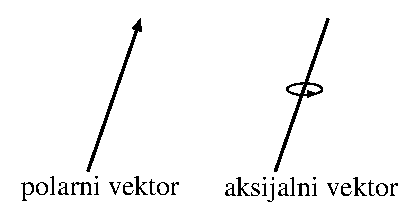
\includegraphics[scale=0.8]{pics/aksijalni_vektor.eps}}

Slično definiramo \emph{pseudoskalarne} veličine kao one koje su skalari
obzirom na rotacije, ali mijenjaju predznak pri refleksijama i inverzijama.
Npr. miješani produkt polarnih vektora je pseudoskalar:

\[
P = (\vec{r}_1 \times \vec{p}) \cdot \vec{r}_2  \; \stackrel{i}{\longrightarrow} \;
  - (\vec{r}_1 \times \vec{p}) \cdot \vec{r}_2 = - P
\]

Magnetski moment, definiran kao $\vec{M} = \frac{1}{2} \int \vec{r}
\times \vec{J} dV$ za gustoću struje $J$, odnosno kao
$\vec{M} = \frac{1}{2} q \vec{r} \times \vec{v}$ za točkasti
naboj $q$, je dakle aksijalni vektor.

Za još o pseudovektorima i drugim pseudo-veličinama vidi
npr. \cite{Arfken:1995}.


\chapter{Kvantna mehanika u Diracovoj notaciji}
\label{sec:qm}

\textbf{Fizikalno stanje} kvantnomehaničkog sustava
je reprezentirano vektorom u Hilbertovom prostoru za
koji se koristi Diracova oznaka
 $\ket{\alpha}$ --- tzv. "ket". 
(Strogo uzevši, kvantnom stanju odgovara
čitava "zraka" $c\ket{\alpha}, c\in\mathbb{C}$.)

Simbol $\alpha$ ovdje stoji za sve kvantne brojeve koji su potrebni za potpuno
određenje stanja. Npr, za vodikov atom $\ket{\alpha}=\ket{n,l,m}$.
Svakom vektoru odgovara dualni "bra" vektor $\bra{\alpha}$, tako
da skalarni produkt zapisujemo kao "bra-ket"A
$\bra{\alpha}\beta \rangle$. Kako je riječ o vektorskom prostoru
nad kompleksnim poljem, vrijedi
$\bra{\alpha}\beta \rangle^{*} = \bra{\beta}\alpha \rangle$.

\textbf{Opservabla} (veličina koja se eksperimentalno određuje i ima
 analogon u klasičnoj fizici) je reprezentirana hermitskim operatorom na
 Hilbertovom prostoru prostoru stanja: $A=A^{\dagger}$.

Ako su $\ket{a}$ svojstveni vektori od $A$ sa svojstvenim vrijednostima
$a$, tj.
\begin{displaymath}
                A\ket{a}=a\ket{a} \;,
\end{displaymath}
onda mjerenje klasične veličine koja odgovara operatoru A, na sustavu
opisanom vektorom $\ket{\alpha}$, s vjerojatnošću $|\bra{a}\alpha\rangle|^2$
ima ishod $a$, nakon čega sustav "skače" u stanje $\ket{a}$.

Očekivana vrijednost mjerenja veličine koja odgovara
operatoru $A$, na sustavu opisanom vektorom stanja
$\ket{\alpha}$ je $\bra{\alpha}A\ket{\alpha}$.

Svi svojstveni vektori nekog hermitskog operatora čine jednu bazu
Hilbertovog prostora:
\begin{displaymath}
             \sum_{a} \ket{a}\bra{a} = 1 \,.
\end{displaymath}
Npr. svi vektori $\ket{\vec{r}}$ čine jednu tzv. koordinatnu bazu.
Schr\"{o}dingerova valna funkcija $\psi_{\alpha}(\vec{r})$ su zapravo
komponente vektora stanja $\ket{\alpha}$ prikazane u koordinatnoj
bazi:
\begin{displaymath}
            \psi_{\alpha}(\vec{r})=\bra{\vec{r}}\alpha\rangle
\end{displaymath}


\textbf{Operatori transformacije} fizikalnog sustava (tj. odgovarajućeg vektora
stanja) moraju biti unitarni i linearni (ili antiunitarni i antilinearni)
\begin{align*}
\text{\sl unitarnost}&:\; \bra{U\alpha}U\beta\rangle = \bra{\alpha}\beta\rangle
   \\
\text{\sl linearnost}&:\; U\big(c_1\ket{\alpha}+c_{2}\ket{\beta}\big)=
  c_1 U\ket{\alpha} + c_{2} U\ket{\beta}
   \\[2ex]
\text{\sl antiunitarnost}&:\; \bra{U\alpha}U\beta\rangle = \bra{\alpha}\beta\rangle^*
  \\
\text{\sl antilinearnost}&:\; U\big(c_1\ket{\alpha}+c_{2}\ket{\beta}\big)=
  c_{1}^* U\ket{\alpha} + c_{2}^* U\ket{\beta}
\end{align*}
Ovo je sadržaj tzv. Wignerovog teorema, a u osnovi
je posljedica zahtjeva za očuvanjem vjerojatnosti i
načela superpozicije u kvantnoj mehanici.



\printbibliography

\end{document}
